\section{曲线}\label{sec:曲线}
\begin{remark}
    本节含有高级内容,第一次阅读时可以跳过。
\end{remark}

虽然三角形可用于表示细小形状来建模细微几何体如头发、皮毛或草地,
但为了更高效地渲染这类物体,拥有专门的\refvar{Shape}{}是值得的,
因为经常出现它们的许多实例。
本节介绍的\refvar{Curve}{}形状即表示
用\keyindex{三次贝塞尔样条}{cubic Bézier spline}{spline样条}建模的细小几何体,
它由四个控制点$\bm p_0,\bm p_1,\bm p_2$和$\bm p_3$定义。
贝塞尔样条穿过第一个和最后一个控制点;
中间点由多项式给出(见\reffig{3.15})
\begin{align}\label{eq:3.3}
    \bm p(u)=(1-u)^3\bm p_0+3(1-u)^2u\bm p_1+3(1-u)u^2\bm p_2+u^3\bm p_3\, .
\end{align}
给定在其他三次基中指定的曲线,例如\keyindex{Hermite样条}{Hermite spline}{spline样条}
\sidenote{译者注:三次Hermite样条
    形如$\bm p(u)=(2u^3-3u^2+1)\bm p_0+(u^3-2u^2+t)\bm m_0+(-2u^3+3u^2)\bm p_1+(u^3-u^2)\bm m_1$,
    其中$\bm p_i$是起点和终点,$\bm m_i$是起点和终点处的切向量,$u\in[0,1]$。},
很容易将其转化为贝塞尔基,所以这里的实现将这一负担留给用户。
如果经常用的话,可以很容易添加该功能。
\begin{figure}[htbp]
    \centering%LaTeX with PSTricks extensions
%%Creator: Inkscape 1.0.1 (3bc2e813f5, 2020-09-07)
%%Please note this file requires PSTricks extensions
\psset{xunit=.35pt,yunit=.35pt,runit=.35pt}
\begin{pspicture}(480,326.66666667)
{
\newrgbcolor{curcolor}{0 0 0}
\pscustom[linewidth=1.33333331,linecolor=curcolor]
{
\newpath
\moveto(9.57291718,164.30208253)
\curveto(162.74478413,317.47395881)(392.50520722,11.13021825)(469.09373936,240.89062667)
}
}
{
\newrgbcolor{curcolor}{0 0 0}
\pscustom[linestyle=none,fillstyle=solid,fillcolor=curcolor]
{
\newpath
\moveto(12.92187447,164.00000253)
\curveto(12.92187447,164.95312252)(12.54687447,165.86458917)(11.86979182,166.53645583)
\curveto(11.19791716,167.21354915)(10.28645851,167.58854914)(9.33333319,167.58854914)
\curveto(8.38020787,167.58854914)(7.46874922,167.21354915)(6.79687456,166.53645583)
\curveto(6.1197919,165.86458917)(5.74479191,164.95312252)(5.74479191,164.00000253)
\curveto(5.74479191,163.04688255)(6.1197919,162.1354159)(6.79687456,161.46354924)
\curveto(7.46874922,160.78645592)(8.38020787,160.41145592)(9.33333319,160.41145592)
\curveto(10.28645851,160.41145592)(11.19791716,160.78645592)(11.86979182,161.46354924)
\curveto(12.54687447,162.1354159)(12.92187447,163.04688255)(12.92187447,164.00000253)
\closepath
\moveto(12.92187447,164.00000253)
}
}
{
\newrgbcolor{curcolor}{0 0 0}
\pscustom[linestyle=none,fillstyle=solid,fillcolor=curcolor]
{
\newpath
\moveto(166.25521074,317.33333348)
\curveto(166.25521074,318.2864588)(165.88021075,319.19791745)(165.20311743,319.86979211)
\curveto(164.53125077,320.54687476)(163.61978412,320.92187476)(162.66666413,320.92187476)
\curveto(161.71354415,320.92187476)(160.8020775,320.54687476)(160.13021084,319.86979211)
\curveto(159.45311752,319.19791745)(159.07811752,318.2864588)(159.07811752,317.33333348)
\curveto(159.07811752,316.38020816)(159.45311752,315.46874951)(160.13021084,314.79687485)
\curveto(160.8020775,314.1197922)(161.71354415,313.7447922)(162.66666413,313.7447922)
\curveto(163.61978412,313.7447922)(164.53125077,314.1197922)(165.20311743,314.79687485)
\curveto(165.88021075,315.46874951)(166.25521074,316.38020816)(166.25521074,317.33333348)
\closepath
\moveto(166.25521074,317.33333348)
}
}
{
\newrgbcolor{curcolor}{0 0 0}
\pscustom[linestyle=none,fillstyle=solid,fillcolor=curcolor]
{
\newpath
\moveto(395.58854051,10.66667159)
\curveto(395.58854051,11.61979157)(395.21354051,12.53125822)(394.53644719,13.20312488)
\curveto(393.86458053,13.8802182)(392.95311388,14.2552182)(391.9999939,14.2552182)
\curveto(391.04687391,14.2552182)(390.13540726,13.8802182)(389.4635406,13.20312488)
\curveto(388.78644728,12.53125822)(388.41144729,11.61979157)(388.41144729,10.66667159)
\curveto(388.41144729,9.7135516)(388.78644728,8.80208495)(389.4635406,8.13021829)
\curveto(390.13540726,7.45312497)(391.04687391,7.07812498)(391.9999939,7.07812498)
\curveto(392.95311388,7.07812498)(393.86458053,7.45312497)(394.53644719,8.13021829)
\curveto(395.21354051,8.80208495)(395.58854051,9.7135516)(395.58854051,10.66667159)
\closepath
\moveto(395.58854051,10.66667159)
}
}
{
\newrgbcolor{curcolor}{0 0 0}
\pscustom[linestyle=none,fillstyle=solid,fillcolor=curcolor]
{
\newpath
\moveto(472.92187264,241.33333466)
\curveto(472.92187264,242.28645998)(472.54687264,243.19791863)(471.86977932,243.86979329)
\curveto(471.19791266,244.54687595)(470.28644601,244.92187594)(469.33332603,244.92187594)
\curveto(468.38020604,244.92187594)(467.46873939,244.54687595)(466.79687273,243.86979329)
\curveto(466.11977941,243.19791863)(465.74477941,242.28645998)(465.74477941,241.33333466)
\curveto(465.74477941,240.38020934)(466.11977941,239.46875069)(466.79687273,238.79687603)
\curveto(467.46873939,238.11979338)(468.38020604,237.74479338)(469.33332603,237.74479338)
\curveto(470.28644601,237.74479338)(471.19791266,238.11979338)(471.86977932,238.79687603)
\curveto(472.54687264,239.46875069)(472.92187264,240.38020934)(472.92187264,241.33333466)
\closepath
\moveto(472.92187264,241.33333466)
}
}
{
\newrgbcolor{curcolor}{0 0 0}
\pscustom[linestyle=none,fillstyle=solid,fillcolor=curcolor]
{
\newpath
\moveto(11.10536797,131.47686588)
\curveto(11.02203463,131.10186588)(10.98036797,131.06019921)(10.9387013,131.01853255)
\curveto(10.8137013,130.97686588)(10.52203464,130.97686588)(10.27203464,130.97686588)
\curveto(9.81370132,130.97686588)(9.31370133,130.97686588)(9.31370133,130.22686589)
\curveto(9.31370133,129.93519923)(9.56370132,129.7268659)(9.85536798,129.7268659)
\curveto(10.60536797,129.7268659)(11.48036796,129.81019923)(12.27203461,129.81019923)
\curveto(13.23036793,129.81019923)(14.23036792,129.7268659)(15.14703457,129.7268659)
\curveto(15.31370123,129.7268659)(15.81370123,129.7268659)(15.81370123,130.51853256)
\curveto(15.81370123,130.97686588)(15.39703456,130.97686588)(15.14703457,130.97686588)
\curveto(14.77203457,130.97686588)(14.31370125,130.97686588)(13.98036792,131.01853255)
\lineto(15.14703457,135.64353248)
\curveto(15.52203456,135.26853248)(16.39703455,134.68519916)(17.81370119,134.68519916)
\curveto(22.43870112,134.68519916)(25.31370108,138.89353243)(25.31370108,142.51853237)
\curveto(25.31370108,145.81019899)(22.85536778,146.8935323)(20.64703448,146.8935323)
\curveto(18.77203451,146.8935323)(17.39703453,145.85186565)(16.98036787,145.47686566)
\curveto(15.93870122,146.8935323)(14.18870125,146.8935323)(13.89703459,146.8935323)
\curveto(12.93870127,146.8935323)(12.14703462,146.35186564)(11.60536796,145.39353233)
\curveto(10.9387013,144.31019901)(10.56370131,142.89353236)(10.56370131,142.76853237)
\curveto(10.56370131,142.39353237)(10.98036797,142.39353237)(11.23036796,142.39353237)
\curveto(11.52203463,142.39353237)(11.60536796,142.39353237)(11.73036796,142.51853237)
\curveto(11.81370129,142.56019904)(11.81370129,142.64353237)(11.98036795,143.31019902)
\curveto(12.48036794,145.43519899)(13.10536793,145.93519898)(13.77203459,145.93519898)
\curveto(14.06370125,145.93519898)(14.39703458,145.85186565)(14.39703458,144.97686566)
\curveto(14.39703458,144.560199)(14.31370125,144.18519901)(14.23036792,143.81019902)
\closepath
\moveto(17.23036787,144.22686568)
\curveto(17.98036786,145.14353233)(19.23036784,145.93519898)(20.52203449,145.93519898)
\curveto(22.18870113,145.93519898)(22.31370112,144.51853234)(22.31370112,143.93519901)
\curveto(22.31370112,142.56019904)(21.39703447,139.26853242)(20.98036781,138.22686577)
\curveto(20.14703449,136.31019913)(18.85536784,135.64353248)(17.77203453,135.64353248)
\curveto(16.18870122,135.64353248)(15.56370123,136.89353246)(15.56370123,137.18519912)
\lineto(15.6053679,137.56019911)
\closepath
\moveto(17.23036787,144.22686568)
}
}
{
\newrgbcolor{curcolor}{0 0 0}
\pscustom[linestyle=none,fillstyle=solid,fillcolor=curcolor]
{
\newpath
\moveto(35.27903295,136.82619034)
\curveto(35.27903295,138.86785697)(35.02903296,140.36785695)(34.19569964,141.65952359)
\curveto(33.61236631,142.49285691)(32.44569966,143.2428569)(30.98736635,143.2428569)
\curveto(26.65403309,143.2428569)(26.65403309,138.15952365)(26.65403309,136.82619034)
\curveto(26.65403309,135.49285702)(26.65403309,130.53452377)(30.98736635,130.53452377)
\curveto(35.27903295,130.53452377)(35.27903295,135.49285702)(35.27903295,136.82619034)
\closepath
\moveto(30.98736635,131.07619043)
\curveto(30.11236637,131.07619043)(28.98736638,131.57619042)(28.61236639,133.07619039)
\curveto(28.36236639,134.15952371)(28.36236639,135.70119035)(28.36236639,137.07619033)
\curveto(28.36236639,138.45119031)(28.36236639,139.86785696)(28.61236639,140.86785694)
\curveto(29.02903305,142.32619025)(30.1956997,142.74285691)(30.98736635,142.74285691)
\curveto(31.98736634,142.74285691)(32.94569966,142.11785692)(33.27903298,141.0345236)
\curveto(33.57069965,140.03452362)(33.61236631,138.70119031)(33.61236631,137.07619033)
\curveto(33.61236631,135.70119035)(33.61236631,134.32619037)(33.36236632,133.15952373)
\curveto(32.98736632,131.45119042)(31.73736634,131.07619043)(30.98736635,131.07619043)
\closepath
\moveto(30.98736635,131.07619043)
}
}
{
\newrgbcolor{curcolor}{0 0 0}
\pscustom[linestyle=none,fillstyle=solid,fillcolor=curcolor]
{
\newpath
\moveto(173.78318677,289.46850075)
\curveto(173.69985343,289.09350075)(173.65818677,289.05183409)(173.6165201,289.01016742)
\curveto(173.4915201,288.96850076)(173.19985344,288.96850076)(172.94985345,288.96850076)
\curveto(172.49152012,288.96850076)(171.99152013,288.96850076)(171.99152013,288.21850077)
\curveto(171.99152013,287.92683411)(172.24152012,287.71850078)(172.53318678,287.71850078)
\curveto(173.28318677,287.71850078)(174.15818676,287.80183411)(174.94985341,287.80183411)
\curveto(175.90818673,287.80183411)(176.90818672,287.71850078)(177.82485337,287.71850078)
\curveto(177.99152003,287.71850078)(178.49152003,287.71850078)(178.49152003,288.51016743)
\curveto(178.49152003,288.96850076)(178.07485337,288.96850076)(177.82485337,288.96850076)
\curveto(177.44985338,288.96850076)(176.99152005,288.96850076)(176.65818672,289.01016742)
\lineto(177.82485337,293.63516735)
\curveto(178.19985336,293.26016736)(179.07485335,292.67683403)(180.49151999,292.67683403)
\curveto(185.11651992,292.67683403)(187.99151988,296.8851673)(187.99151988,300.51016724)
\curveto(187.99151988,303.80183386)(185.53318658,304.88516718)(183.32485328,304.88516718)
\curveto(181.44985331,304.88516718)(180.07485333,303.84350052)(179.65818667,303.46850053)
\curveto(178.61652002,304.88516718)(176.86652005,304.88516718)(176.57485339,304.88516718)
\curveto(175.61652007,304.88516718)(174.82485342,304.34350052)(174.28318676,303.3851672)
\curveto(173.6165201,302.30183388)(173.24152011,300.88516724)(173.24152011,300.76016724)
\curveto(173.24152011,300.38516725)(173.65818677,300.38516725)(173.90818676,300.38516725)
\curveto(174.19985343,300.38516725)(174.28318676,300.38516725)(174.40818676,300.51016724)
\curveto(174.49152009,300.55183391)(174.49152009,300.63516724)(174.65818675,301.3018339)
\curveto(175.15818674,303.42683386)(175.78318673,303.92683386)(176.44985339,303.92683386)
\curveto(176.74152005,303.92683386)(177.07485338,303.84350052)(177.07485338,302.96850054)
\curveto(177.07485338,302.55183388)(176.99152005,302.17683388)(176.90818672,301.80183389)
\closepath
\moveto(179.90818667,302.21850055)
\curveto(180.65818666,303.1351672)(181.90818664,303.92683386)(183.19985329,303.92683386)
\curveto(184.86651993,303.92683386)(184.99151992,302.51016721)(184.99151992,301.92683389)
\curveto(184.99151992,300.55183391)(184.07485327,297.26016729)(183.65818661,296.21850064)
\curveto(182.82485329,294.30183401)(181.53318664,293.63516735)(180.44985333,293.63516735)
\curveto(178.86652002,293.63516735)(178.24152003,294.88516733)(178.24152003,295.17683399)
\lineto(178.2831867,295.55183399)
\closepath
\moveto(179.90818667,302.21850055)
}
}
{
\newrgbcolor{curcolor}{0 0 0}
\pscustom[linestyle=none,fillstyle=solid,fillcolor=curcolor]
{
\newpath
\moveto(194.58185181,300.73449178)
\curveto(194.58185181,301.23449178)(194.58185181,301.23449178)(194.04018515,301.23449178)
\curveto(192.83185183,300.06782513)(191.16518519,300.06782513)(190.4151852,300.06782513)
\lineto(190.4151852,299.40115847)
\curveto(190.83185186,299.40115847)(192.08185185,299.40115847)(193.08185183,299.90115846)
\lineto(193.08185183,290.44282528)
\curveto(193.08185183,289.81782529)(193.08185183,289.56782529)(191.24851852,289.56782529)
\lineto(190.5401852,289.56782529)
\lineto(190.5401852,288.90115863)
\curveto(190.87351853,288.90115863)(193.16518516,288.98449197)(193.83185182,288.98449197)
\curveto(194.41518514,288.98449197)(196.74851844,288.90115863)(197.1651851,288.90115863)
\lineto(197.1651851,289.56782529)
\lineto(196.45685178,289.56782529)
\curveto(194.58185181,289.56782529)(194.58185181,289.81782529)(194.58185181,290.44282528)
\closepath
\moveto(194.58185181,300.73449178)
}
}
{
\newrgbcolor{curcolor}{0 0 0}
\pscustom[linestyle=none,fillstyle=solid,fillcolor=curcolor]
{
\newpath
\moveto(365.91707177,21.01661426)
\curveto(365.83373844,20.64161427)(365.79207178,20.5999476)(365.75040511,20.55828094)
\curveto(365.62540511,20.51661427)(365.33373845,20.51661427)(365.08373845,20.51661427)
\curveto(364.62540513,20.51661427)(364.12540514,20.51661427)(364.12540514,19.76661428)
\curveto(364.12540514,19.47494762)(364.37540513,19.26661429)(364.66707179,19.26661429)
\curveto(365.41707178,19.26661429)(366.29207177,19.34994762)(367.08373842,19.34994762)
\curveto(368.04207174,19.34994762)(369.04207173,19.26661429)(369.95873838,19.26661429)
\curveto(370.12540504,19.26661429)(370.62540503,19.26661429)(370.62540503,20.05828094)
\curveto(370.62540503,20.51661427)(370.20873837,20.51661427)(369.95873838,20.51661427)
\curveto(369.58373838,20.51661427)(369.12540506,20.51661427)(368.79207173,20.55828094)
\lineto(369.95873838,25.18328086)
\curveto(370.33373837,24.80828087)(371.20873836,24.22494755)(372.625405,24.22494755)
\curveto(377.25040493,24.22494755)(380.12540489,28.43328081)(380.12540489,32.05828076)
\curveto(380.12540489,35.34994737)(377.66707159,36.43328069)(375.45873829,36.43328069)
\curveto(373.58373832,36.43328069)(372.20873834,35.39161404)(371.79207168,35.01661404)
\curveto(370.75040503,36.43328069)(369.00040506,36.43328069)(368.7087384,36.43328069)
\curveto(367.75040508,36.43328069)(366.95873842,35.89161403)(366.41707177,34.93328071)
\curveto(365.75040511,33.8499474)(365.37540512,32.43328075)(365.37540512,32.30828075)
\curveto(365.37540512,31.93328076)(365.79207178,31.93328076)(366.04207177,31.93328076)
\curveto(366.33373843,31.93328076)(366.41707177,31.93328076)(366.54207176,32.05828076)
\curveto(366.6254051,32.09994742)(366.6254051,32.18328075)(366.79207176,32.84994741)
\curveto(367.29207175,34.97494738)(367.91707174,35.47494737)(368.5837384,35.47494737)
\curveto(368.87540506,35.47494737)(369.20873839,35.39161404)(369.20873839,34.51661405)
\curveto(369.20873839,34.09994739)(369.12540506,33.7249474)(369.04207173,33.3499474)
\closepath
\moveto(372.04207168,33.76661406)
\curveto(372.79207167,34.68328072)(374.04207165,35.47494737)(375.33373829,35.47494737)
\curveto(377.00040493,35.47494737)(377.12540493,34.05828073)(377.12540493,33.4749474)
\curveto(377.12540493,32.09994742)(376.20873828,28.80828081)(375.79207162,27.76661416)
\curveto(374.9587383,25.84994752)(373.66707165,25.18328086)(372.58373834,25.18328086)
\curveto(371.00040503,25.18328086)(370.37540504,26.43328084)(370.37540504,26.72494751)
\lineto(370.4170717,27.0999475)
\closepath
\moveto(372.04207168,33.76661406)
}
}
{
\newrgbcolor{curcolor}{0 0 0}
\pscustom[linestyle=none,fillstyle=solid,fillcolor=curcolor]
{
\newpath
\moveto(389.88240343,23.8242721)
\lineto(389.25740344,23.8242721)
\curveto(389.21573678,23.40760544)(389.00740345,22.32427212)(388.75740345,22.15760545)
\curveto(388.63240345,22.03260546)(387.21573681,22.03260546)(386.92407014,22.03260546)
\lineto(383.50740353,22.03260546)
\curveto(385.46573683,23.74093876)(386.13240349,24.28260542)(387.21573681,25.15760541)
\curveto(388.59073679,26.24093872)(389.88240343,27.40760537)(389.88240343,29.15760535)
\curveto(389.88240343,31.40760531)(387.92407013,32.78260529)(385.54907017,32.78260529)
\curveto(383.25740354,32.78260529)(381.67407023,31.15760531)(381.67407023,29.44927201)
\curveto(381.67407023,28.53260536)(382.46573688,28.40760536)(382.67407021,28.40760536)
\curveto(383.09073687,28.40760536)(383.63240353,28.74093869)(383.63240353,29.40760534)
\curveto(383.63240353,29.74093867)(383.50740353,30.40760533)(382.54907021,30.40760533)
\curveto(383.13240354,31.69927197)(384.38240352,32.11593863)(385.2574035,32.11593863)
\curveto(387.13240347,32.11593863)(388.09073679,30.65760532)(388.09073679,29.15760535)
\curveto(388.09073679,27.53260537)(386.92407014,26.28260539)(386.34073682,25.61593873)
\lineto(381.88240356,21.15760547)
\curveto(381.67407023,20.99093881)(381.67407023,20.94927214)(381.67407023,20.44927215)
\lineto(389.34073677,20.44927215)
\closepath
\moveto(389.88240343,23.8242721)
}
}
{
\newrgbcolor{curcolor}{0 0 0}
\pscustom[linestyle=none,fillstyle=solid,fillcolor=curcolor]
{
\newpath
\moveto(436.20996135,245.28439477)
\curveto(436.12662801,244.90939478)(436.08496135,244.86772811)(436.04329468,244.82606144)
\curveto(435.91829468,244.78439478)(435.62662802,244.78439478)(435.37662803,244.78439478)
\curveto(434.9182947,244.78439478)(434.41829471,244.78439478)(434.41829471,244.03439479)
\curveto(434.41829471,243.74272813)(434.6682947,243.5343948)(434.95996137,243.5343948)
\curveto(435.70996135,243.5343948)(436.58496134,243.61772813)(437.37662799,243.61772813)
\curveto(438.33496131,243.61772813)(439.3349613,243.5343948)(440.25162795,243.5343948)
\curveto(440.41829461,243.5343948)(440.91829461,243.5343948)(440.91829461,244.32606145)
\curveto(440.91829461,244.78439478)(440.50162795,244.78439478)(440.25162795,244.78439478)
\curveto(439.87662796,244.78439478)(439.41829463,244.78439478)(439.0849613,244.82606144)
\lineto(440.25162795,249.45106137)
\curveto(440.62662794,249.07606138)(441.50162793,248.49272805)(442.91829458,248.49272805)
\curveto(447.5432945,248.49272805)(450.41829446,252.70106132)(450.41829446,256.32606126)
\curveto(450.41829446,259.61772788)(447.95996116,260.7010612)(445.75162786,260.7010612)
\curveto(443.87662789,260.7010612)(442.50162791,259.65939455)(442.08496125,259.28439455)
\curveto(441.0432946,260.7010612)(439.29329463,260.7010612)(439.00162797,260.7010612)
\curveto(438.04329465,260.7010612)(437.251628,260.15939454)(436.70996134,259.20106122)
\curveto(436.04329468,258.1177279)(435.66829469,256.70106126)(435.66829469,256.57606126)
\curveto(435.66829469,256.20106127)(436.08496135,256.20106127)(436.33496134,256.20106127)
\curveto(436.62662801,256.20106127)(436.70996134,256.20106127)(436.83496134,256.32606126)
\curveto(436.91829467,256.36772793)(436.91829467,256.45106126)(437.08496133,257.11772792)
\curveto(437.58496132,259.24272789)(438.20996132,259.74272788)(438.87662797,259.74272788)
\curveto(439.16829463,259.74272788)(439.50162796,259.65939455)(439.50162796,258.78439456)
\curveto(439.50162796,258.3677279)(439.41829463,257.99272791)(439.3349613,257.61772791)
\closepath
\moveto(442.33496125,258.03439457)
\curveto(443.08496124,258.95106122)(444.33496122,259.74272788)(445.62662787,259.74272788)
\curveto(447.29329451,259.74272788)(447.4182945,258.32606123)(447.4182945,257.74272791)
\curveto(447.4182945,256.36772793)(446.50162785,253.07606132)(446.08496119,252.03439466)
\curveto(445.25162787,250.11772803)(443.95996123,249.45106137)(442.87662791,249.45106137)
\curveto(441.2932946,249.45106137)(440.66829461,250.70106135)(440.66829461,250.99272801)
\lineto(440.70996128,251.36772801)
\closepath
\moveto(442.33496125,258.03439457)
}
}
{
\newrgbcolor{curcolor}{0 0 0}
\pscustom[linestyle=none,fillstyle=solid,fillcolor=curcolor]
{
\newpath
\moveto(455.8836264,250.92538589)
\curveto(457.34195972,250.92538589)(458.38362637,249.92538591)(458.38362637,247.92538594)
\curveto(458.38362637,245.63371931)(457.00862639,244.92538599)(455.96695974,244.92538599)
\curveto(455.21695975,244.92538599)(453.55029311,245.13371932)(452.80029312,246.2587193)
\curveto(453.67529311,246.2587193)(453.88362644,246.88371929)(453.88362644,247.30038595)
\curveto(453.88362644,247.88371927)(453.42529311,248.30038593)(452.84195979,248.30038593)
\curveto(452.34195979,248.30038593)(451.80029313,247.96705261)(451.80029313,247.21705262)
\curveto(451.80029313,245.46705264)(453.71695977,244.34205266)(455.96695974,244.34205266)
\curveto(458.55029303,244.34205266)(460.34195967,246.09205263)(460.34195967,247.92538594)
\curveto(460.34195967,249.38371925)(459.17529302,250.84205256)(457.13362638,251.25871922)
\curveto(459.05029302,251.96705254)(459.75862634,253.34205252)(459.75862634,254.50871917)
\curveto(459.75862634,255.96705248)(458.0919597,257.0503858)(456.0086264,257.0503858)
\curveto(453.96695977,257.0503858)(452.38362646,256.05038581)(452.38362646,254.55038584)
\curveto(452.38362646,253.92538585)(452.80029312,253.59205252)(453.34195978,253.59205252)
\curveto(453.9252931,253.59205252)(454.3002931,254.00871918)(454.3002931,254.50871917)
\curveto(454.3002931,255.05038583)(453.9252931,255.46705249)(453.34195978,255.50871915)
\curveto(454.00862643,256.30038581)(455.25862641,256.50871914)(455.96695974,256.50871914)
\curveto(456.80029306,256.50871914)(457.96695971,256.09205248)(457.96695971,254.50871917)
\curveto(457.96695971,253.71705252)(457.71695971,252.84205253)(457.21695972,252.30038587)
\curveto(456.63362639,251.59205255)(456.09195973,251.55038588)(455.17529308,251.46705255)
\curveto(454.71695976,251.42538589)(454.67529309,251.42538589)(454.59195976,251.42538589)
\curveto(454.55029309,251.42538589)(454.38362643,251.38371922)(454.38362643,251.17538589)
\curveto(454.38362643,250.92538589)(454.55029309,250.92538589)(454.88362642,250.92538589)
\closepath
\moveto(455.8836264,250.92538589)
}
}
\end{pspicture}

    \caption{三次贝塞尔曲线由四个控制点$\bm p_i$定义。
        \protect\refeq{3.3}定义的曲线$\bm p(u)$分别在$u=0$和$u=1$处穿过第一个和最后一个控制点。}
    \label{fig:3.15}
\end{figure}

\refvar{Curve}{}形状由具有宽度的1D贝塞尔曲线定义,
其宽度是从起点宽度到终点宽度沿其范围线性插值的。
即它们定义了一个平坦的2D曲面(\reffig{3.16})
\footnote{注意术语的滥用:尽管曲线是1D数学概念,但\protect\refvar{Curve}{}形状表示2D曲面。
    下文中我们所称的曲线通常指\protect\refvar{Shape}{}。
    当区别不够明确时我们用“贝塞尔曲线”来区分1D概念。}。
直接用光线与该表示相交而不用细化\sidenote{译者注:原文tessellating。}它是可能的,
从而能够高效渲染平滑曲线而不使用过多内存。
\begin{figure}[htbp]
    \centering%LaTeX with PSTricks extensions
%%Creator: Inkscape 1.0.1 (3bc2e813f5, 2020-09-07)
%%Please note this file requires PSTricks extensions
\psset{xunit=.5pt,yunit=.5pt,runit=.5pt}
\begin{pspicture}(480,137.33333333)
{
\newrgbcolor{curcolor}{0 0 0}
\pscustom[linestyle=none,fillstyle=solid,fillcolor=curcolor]
{
\newpath
\moveto(3.44791727,32.57563467)
\lineto(0.0625,43.63813447)
\lineto(1.99999996,43.63813447)
\lineto(3.76041593,37.25271725)
\lineto(4.41666658,34.8777173)
\curveto(4.44270792,34.99750929)(4.63541591,35.75792661)(4.98958391,37.15896792)
\lineto(6.74999988,43.63813447)
\lineto(8.67708251,43.63813447)
\lineto(10.33333314,37.22146792)
\lineto(10.8854158,35.10688529)
\lineto(11.52083312,37.24230125)
\lineto(13.41666642,43.63813447)
\lineto(15.23958372,43.63813447)
\lineto(11.78125045,32.57563467)
\lineto(9.83333315,32.57563467)
\lineto(8.07291718,39.20063455)
\lineto(7.64583319,41.08605051)
\lineto(5.40625057,32.57563467)
\closepath
\moveto(3.44791727,32.57563467)
}
}
{
\newrgbcolor{curcolor}{0 0 0}
\pscustom[linestyle=none,fillstyle=solid,fillcolor=curcolor]
{
\newpath
\moveto(16.82291763,45.69021843)
\lineto(16.82291763,47.84646772)
\lineto(18.69791759,47.84646772)
\lineto(18.69791759,45.69021843)
\closepath
\moveto(16.82291763,32.57563467)
\lineto(16.82291763,43.63813447)
\lineto(18.69791759,43.63813447)
\lineto(18.69791759,32.57563467)
\closepath
\moveto(16.82291763,32.57563467)
}
}
{
\newrgbcolor{curcolor}{0 0 0}
\pscustom[linestyle=none,fillstyle=solid,fillcolor=curcolor]
{
\newpath
\moveto(28.72916613,32.57563467)
\lineto(28.72916613,33.97146798)
\curveto(28.02604081,32.87250933)(26.9947915,32.32563468)(25.63541686,32.32563468)
\curveto(24.75520754,32.32563468)(23.94270756,32.57042634)(23.2031249,33.05480133)
\curveto(22.46354092,33.53917599)(21.89062493,34.22146797)(21.48437427,35.09125996)
\curveto(21.07812494,35.96105061)(20.87499961,36.96625992)(20.87499961,38.0964679)
\curveto(20.87499961,39.20063455)(21.05729161,40.20063453)(21.4270836,41.10167585)
\curveto(21.79687426,42.00271716)(22.34895825,42.69021848)(23.08333291,43.16938381)
\curveto(23.81770756,43.6485518)(24.64062488,43.88813446)(25.55208353,43.88813446)
\curveto(26.21875018,43.88813446)(26.8124995,43.74750913)(27.33333283,43.4662598)
\curveto(27.85416615,43.18500914)(28.27604081,42.82042648)(28.60416614,42.36730116)
\lineto(28.60416614,47.84646772)
\lineto(30.4687501,47.84646772)
\lineto(30.4687501,32.57563467)
\closepath
\moveto(22.80208358,38.0964679)
\curveto(22.80208358,36.67980126)(23.09895824,35.62250928)(23.69791556,34.91938396)
\curveto(24.29687422,34.21625997)(24.99999954,33.86730131)(25.81249952,33.86730131)
\curveto(26.63020751,33.86730131)(27.32812483,34.20063464)(27.90104082,34.8725093)
\curveto(28.47395814,35.54438395)(28.7604168,36.5652186)(28.7604168,37.94021857)
\curveto(28.7604168,39.45584254)(28.46875014,40.56521852)(27.88541682,41.27355184)
\curveto(27.30208349,41.98188516)(26.58333284,42.33605049)(25.72916619,42.33605049)
\curveto(24.89583287,42.33605049)(24.19791555,41.99750916)(23.6406249,41.31521851)
\curveto(23.08333291,40.63292652)(22.80208358,39.56000921)(22.80208358,38.0964679)
\closepath
\moveto(22.80208358,38.0964679)
}
}
{
\newrgbcolor{curcolor}{0 0 0}
\pscustom[linestyle=none,fillstyle=solid,fillcolor=curcolor]
{
\newpath
\moveto(37.51041597,34.25271731)
\lineto(37.7812493,32.596468)
\curveto(37.25520798,32.48709307)(36.78124932,32.42980134)(36.36458266,32.42980134)
\curveto(35.68229067,32.42980134)(35.15624935,32.53917627)(34.78124936,32.75271733)
\curveto(34.40624936,32.96626)(34.14062403,33.25271733)(33.9895827,33.60167599)
\curveto(33.83854137,33.95063465)(33.76041604,34.69021863)(33.76041604,35.81521861)
\lineto(33.76041604,42.17980116)
\lineto(32.38541607,42.17980116)
\lineto(32.38541607,43.63813447)
\lineto(33.76041604,43.63813447)
\lineto(33.76041604,46.37771708)
\lineto(35.62500001,47.50271706)
\lineto(35.62500001,43.63813447)
\lineto(37.51041597,43.63813447)
\lineto(37.51041597,42.17980116)
\lineto(35.62500001,42.17980116)
\lineto(35.62500001,35.71105061)
\curveto(35.62500001,35.17459329)(35.65624934,34.83084263)(35.72395734,34.6798013)
\curveto(35.79166667,34.52875997)(35.895832,34.40375997)(36.04687467,34.31521864)
\curveto(36.197916,34.22667597)(36.41145733,34.17980131)(36.68749865,34.17980131)
\curveto(36.89583198,34.17980131)(37.17187464,34.20584264)(37.51041597,34.25271731)
\closepath
\moveto(37.51041597,34.25271731)
}
}
{
\newrgbcolor{curcolor}{0 0 0}
\pscustom[linestyle=none,fillstyle=solid,fillcolor=curcolor]
{
\newpath
\moveto(39.34374994,32.57563467)
\lineto(39.34374994,47.84646772)
\lineto(41.2187499,47.84646772)
\lineto(41.2187499,42.36730116)
\curveto(42.09374989,43.38292647)(43.1979152,43.88813446)(44.53124851,43.88813446)
\curveto(45.34895783,43.88813446)(46.06249915,43.7266758)(46.6666658,43.4037598)
\curveto(47.27083246,43.08084248)(47.70312445,42.63292648)(47.96354045,42.0652185)
\curveto(48.22395777,41.49750917)(48.35416577,40.66938385)(48.35416577,39.58605054)
\lineto(48.35416577,32.57563467)
\lineto(46.47916581,32.57563467)
\lineto(46.47916581,39.58605054)
\curveto(46.47916581,40.52355186)(46.27604048,41.20584251)(45.86979115,41.6329265)
\curveto(45.46354049,42.06000916)(44.8906245,42.27355182)(44.14583252,42.27355182)
\curveto(43.58854053,42.27355182)(43.0677072,42.12771716)(42.57812454,41.84125983)
\curveto(42.08854055,41.55480117)(41.73958189,41.16417585)(41.53124856,40.66938385)
\curveto(41.32291523,40.1745932)(41.2187499,39.49750921)(41.2187499,38.62771723)
\lineto(41.2187499,32.57563467)
\closepath
\moveto(39.34374994,32.57563467)
}
}
{
\newrgbcolor{curcolor}{0.36078432 0.49803922 0.7019608}
\pscustom[linewidth=2.13333333,linecolor=curcolor]
{
\newpath
\moveto(50.54687373,53.51562689)
\lineto(50.66145773,53.63541755)
\lineto(50.78124973,53.75000155)
\lineto(51.02083239,53.98958554)
\lineto(51.49999905,54.45833487)
\lineto(52.45312436,55.39062685)
\lineto(54.37499899,57.21354282)
\lineto(58.23958292,60.69270942)
\lineto(66.73437343,67.50520929)
\lineto(74.81249861,72.99479319)
\lineto(74.93229061,73.07291852)
\lineto(75.05729061,73.15104252)
\lineto(75.30729061,73.30208385)
\lineto(75.8072906,73.60937585)
\lineto(76.80729058,74.2187505)
\lineto(78.81249854,75.39062648)
\lineto(82.84895713,77.60416777)
\lineto(82.98437313,77.67187577)
\lineto(83.12499846,77.7447931)
\lineto(83.39583179,77.8854171)
\lineto(83.94791578,78.17187576)
\lineto(85.04687309,78.72395975)
\lineto(87.25520638,79.79166773)
\lineto(91.6927063,81.77604236)
\lineto(91.82291563,81.83333436)
\lineto(91.95312363,81.88541703)
\lineto(92.21353963,81.99479302)
\lineto(92.73437295,82.20833435)
\lineto(93.7760396,82.63020901)
\lineto(95.86458222,83.442709)
\lineto(95.99479022,83.494793)
\lineto(96.12499822,83.54166766)
\lineto(96.38541422,83.64062633)
\lineto(96.91145687,83.83333432)
\lineto(97.95833152,84.21354232)
\lineto(100.05729015,84.93750097)
\lineto(100.19791548,84.98437564)
\lineto(100.34374748,85.03645964)
\lineto(100.62499814,85.13020897)
\lineto(101.19791546,85.31770896)
\lineto(102.33853944,85.67708362)
\lineto(104.63020606,86.36979294)
\lineto(104.77603939,86.41145961)
\lineto(104.91666472,86.45312628)
\lineto(105.20312339,86.53645961)
\lineto(105.77603937,86.69791827)
\lineto(106.92708069,87.01562627)
\lineto(109.22916464,87.61458492)
\lineto(109.36978997,87.65104225)
\lineto(109.51562331,87.68229292)
\lineto(109.79687263,87.75520892)
\lineto(110.36458196,87.89062625)
\lineto(111.49478994,88.15625158)
\lineto(113.77083123,88.65625157)
\lineto(113.91145656,88.6822929)
\lineto(114.05728989,88.71354223)
\lineto(114.33853922,88.77083423)
\lineto(114.91145654,88.8854169)
\lineto(116.04687252,89.10937556)
\lineto(118.33333114,89.52604222)
\lineto(118.46874714,89.54687555)
\lineto(118.59895647,89.56770888)
\lineto(118.8697898,89.61458488)
\lineto(119.40103912,89.70312622)
\lineto(120.4687471,89.86979288)
\lineto(120.73958176,89.91145954)
\lineto(121.00520576,89.95312621)
\lineto(121.54166442,90.03125154)
\lineto(122.6093724,90.18750087)
\lineto(122.74478973,90.20312621)
\lineto(122.88020572,90.22395954)
\lineto(123.14583105,90.26041687)
\lineto(124.75520569,90.4635422)
\lineto(126.90624832,90.7083342)
\lineto(127.19791498,90.73958486)
\lineto(127.48958164,90.7656262)
\lineto(128.07291496,90.82291819)
\lineto(129.23958161,90.93229286)
\lineto(129.3854136,90.94791819)
\lineto(129.53124827,90.95833419)
\lineto(129.82291493,90.98437552)
\lineto(130.41145625,91.03125152)
\lineto(131.5781229,91.11979286)
\lineto(131.72916423,91.13020886)
\lineto(132.74999754,91.20312619)
\lineto(132.90103887,91.20833419)
\lineto(133.33853886,91.23958485)
\lineto(133.92708019,91.27083419)
\lineto(134.07291485,91.28125152)
\lineto(134.21874685,91.28645952)
\lineto(134.51041351,91.30208352)
\lineto(135.09895616,91.33333419)
\lineto(135.39062283,91.34375018)
\lineto(135.68749749,91.35937552)
\lineto(136.27603881,91.38541685)
\lineto(136.54687214,91.39583418)
\lineto(136.8229148,91.40625152)
\lineto(137.37499746,91.42187552)
\lineto(137.64583078,91.43229285)
\lineto(137.92187211,91.44270885)
\lineto(138.4739561,91.45312618)
\lineto(138.74478943,91.46354218)
\lineto(139.02083076,91.46875018)
\lineto(139.15624809,91.47395952)
\lineto(139.29687209,91.47395952)
\lineto(139.57291475,91.47916752)
\lineto(139.70833075,91.48437552)
\lineto(139.98437207,91.48437552)
\lineto(140.11978941,91.48958485)
\lineto(140.2604134,91.48958485)
\lineto(140.39583073,91.49479285)
\lineto(140.67187206,91.49479285)
\lineto(140.80728939,91.50000085)
\lineto(141.22395605,91.50000085)
\lineto(141.35937205,91.50520885)
\lineto(143.56249734,91.50520885)
\lineto(143.70312267,91.50000085)
\lineto(144.11458133,91.50000085)
\lineto(144.25520533,91.49479285)
\lineto(144.66666399,91.49479285)
\lineto(144.80728932,91.48958485)
\lineto(145.08333065,91.48437552)
\lineto(145.35416398,91.48437552)
\lineto(145.6249973,91.47916752)
\lineto(145.7604133,91.47395952)
\lineto(145.89583063,91.47395952)
\lineto(146.16666396,91.46354218)
\lineto(146.30207996,91.46354218)
\lineto(146.43749729,91.45833418)
\lineto(146.70833062,91.45312618)
\lineto(147.24999727,91.43750085)
\lineto(147.38541327,91.43229285)
\lineto(147.5208306,91.43229285)
\lineto(147.79166393,91.42187552)
\lineto(148.33333059,91.40625152)
\lineto(149.4166639,91.36458485)
\lineto(149.55728923,91.35937552)
\lineto(149.69270523,91.34895952)
\lineto(149.96353856,91.33854219)
\lineto(150.50520521,91.31250085)
\lineto(151.59374653,91.26041685)
\lineto(151.72916386,91.25000085)
\lineto(151.86458119,91.24479285)
\lineto(152.67707984,91.19791819)
\lineto(153.76562249,91.13020886)
\lineto(153.91145582,91.11979286)
\lineto(154.06249715,91.10937552)
\lineto(154.35416381,91.08854219)
\lineto(154.94791446,91.04687552)
\lineto(156.13020511,90.95833419)
\lineto(156.42187177,90.93750086)
\lineto(156.71874643,90.91145953)
\lineto(157.31249709,90.86458486)
\lineto(158.49478907,90.76041686)
\lineto(158.6406224,90.75000086)
\lineto(158.79166373,90.73437553)
\lineto(159.08333039,90.7083342)
\lineto(159.67707971,90.6510422)
\lineto(160.86458102,90.53125153)
\lineto(163.23437164,90.2760422)
\lineto(163.36978897,90.26041687)
\lineto(163.51041297,90.24479287)
\lineto(163.78645563,90.21354221)
\lineto(164.33853829,90.14583421)
\lineto(165.44791427,90.01041688)
\lineto(167.66145556,89.72395955)
\lineto(167.80207956,89.70312622)
\lineto(167.93749689,89.68750088)
\lineto(168.21353822,89.64583422)
\lineto(168.77083021,89.56770888)
\lineto(169.88020485,89.41145955)
\lineto(172.09895548,89.07812623)
\lineto(172.24999681,89.05729289)
\lineto(172.39583014,89.03125156)
\lineto(173.30207946,88.89062623)
\lineto(174.50520477,88.6927089)
\lineto(176.91145539,88.28125158)
\lineto(181.7291633,87.39062626)
\lineto(181.88020463,87.36458493)
\lineto(182.02603796,87.33333426)
\lineto(182.91666328,87.1614596)
\lineto(184.09895526,86.9218756)
\lineto(186.46353788,86.43229294)
\lineto(191.20312179,85.3906263)
\lineto(200.04166296,83.250001)
\lineto(209.61978812,80.68229305)
\lineto(218.54166262,78.08854243)
\lineto(228.18749577,75.11458515)
\lineto(237.6145796,72.07812654)
\lineto(246.36457944,69.17708393)
\lineto(255.79166193,66.00520932)
\lineto(264.53124577,63.05729338)
\lineto(273.03124561,60.22916809)
\lineto(282.16145344,57.26041748)
\lineto(290.58853595,54.63020953)
\lineto(299.61457845,51.97916825)
\lineto(308.34895296,49.61979362)
\lineto(316.38020214,47.68229366)
\lineto(316.65103547,47.61979366)
\lineto(316.9166608,47.56250166)
\lineto(317.45832745,47.44270966)
\lineto(318.53645277,47.203127)
\lineto(320.68228606,46.75000168)
\lineto(324.94270198,45.91146036)
\lineto(325.06770198,45.88541769)
\lineto(325.19270198,45.86458569)
\lineto(325.44270197,45.81770969)
\lineto(325.93228596,45.72396036)
\lineto(326.92186861,45.55208437)
\lineto(328.89061924,45.21354304)
\lineto(329.01561924,45.19270971)
\lineto(329.13540991,45.17187637)
\lineto(329.3802019,45.13020971)
\lineto(330.84895254,44.89583505)
\lineto(332.8020765,44.60416838)
\lineto(332.9218685,44.58854305)
\lineto(333.0364525,44.57291905)
\lineto(333.27603516,44.53646039)
\lineto(333.75520182,44.46875105)
\lineto(334.70311914,44.34375106)
\lineto(336.59895243,44.10416839)
\lineto(336.7187431,44.08854306)
\lineto(336.8333271,44.07291906)
\lineto(337.06770176,44.04687639)
\lineto(337.54166042,43.98958573)
\lineto(338.4843684,43.88541773)
\lineto(340.35936836,43.69270973)
\lineto(340.48436836,43.68229373)
\lineto(340.61457769,43.6718764)
\lineto(340.86457769,43.64583507)
\lineto(341.37499368,43.5989604)
\lineto(342.38540966,43.51562707)
\lineto(342.63540966,43.49479374)
\lineto(342.89061898,43.4739604)
\lineto(343.39582697,43.43750174)
\lineto(344.40103496,43.36458574)
\lineto(344.52603495,43.35937641)
\lineto(344.65103495,43.34896041)
\lineto(345.40103494,43.30208441)
\lineto(345.52603493,43.29687641)
\lineto(345.65103493,43.28646041)
\lineto(345.90103493,43.27604308)
\lineto(346.40103492,43.24479374)
\lineto(346.90103491,43.22396041)
\lineto(347.4010349,43.19791908)
\lineto(347.5260349,43.19270974)
\lineto(347.6458269,43.18750174)
\lineto(347.89582689,43.17708441)
\lineto(348.39582688,43.16146041)
\lineto(348.62499354,43.15104308)
\lineto(348.85416021,43.14583508)
\lineto(348.9739522,43.14062708)
\lineto(349.08853487,43.13541774)
\lineto(349.31770153,43.13020974)
\lineto(349.43228553,43.13020974)
\lineto(349.54686819,43.12500174)
\lineto(349.78124419,43.11979374)
\lineto(349.89582685,43.11458574)
\lineto(350.01040952,43.11458574)
\lineto(350.23957751,43.10937641)
\lineto(350.35416018,43.10416841)
\lineto(350.58853484,43.10416841)
\lineto(350.70311884,43.09896041)
\lineto(350.9322855,43.09896041)
\lineto(351.16145216,43.09375108)
\lineto(351.27603483,43.09375108)
\lineto(351.39061883,43.08854308)
\lineto(351.96353482,43.08854308)
\lineto(352.07811881,43.08333508)
\lineto(352.99478546,43.08333508)
\lineto(353.10936813,43.08854308)
\lineto(353.67707612,43.08854308)
\lineto(353.79166012,43.09375108)
\lineto(354.13540944,43.09375108)
\lineto(354.24478544,43.09896041)
\lineto(354.4739521,43.09896041)
\lineto(354.58853477,43.10416841)
\lineto(354.81249343,43.10937641)
\lineto(355.04166009,43.10937641)
\lineto(355.27082675,43.11979374)
\lineto(355.72395208,43.13020974)
\lineto(355.84374274,43.13541774)
\lineto(355.96874274,43.13541774)
\lineto(356.21353474,43.14583508)
\lineto(356.33332673,43.15104308)
\lineto(356.45832673,43.15104308)
\lineto(356.70311873,43.16146041)
\lineto(356.82291073,43.16666841)
\lineto(356.94791072,43.17187641)
\lineto(357.19270139,43.18229374)
\lineto(357.67707604,43.20312708)
\lineto(357.80207604,43.20833508)
\lineto(357.92186804,43.21354308)
\lineto(358.16666003,43.22916841)
\lineto(358.65103469,43.25520974)
\lineto(359.62499334,43.31250174)
\lineto(359.86457734,43.33333507)
\lineto(360.109368,43.34896041)
\lineto(360.58853466,43.38541774)
\lineto(361.55207597,43.46354307)
\lineto(361.67707597,43.4739604)
\lineto(362.03645196,43.50520974)
\lineto(362.51561862,43.5520844)
\lineto(363.47395194,43.65104307)
\lineto(363.5833266,43.6614604)
\lineto(363.6979106,43.6770844)
\lineto(363.91665993,43.69791907)
\lineto(364.36457725,43.75000173)
\lineto(365.24999324,43.8593764)
\lineto(365.36457723,43.87500173)
\lineto(365.4739519,43.89062706)
\lineto(365.69270123,43.9166684)
\lineto(367.02082654,44.10416839)
\lineto(367.2395772,44.13541773)
\lineto(367.45832653,44.17187639)
\lineto(367.90103452,44.23958572)
\lineto(368.7760345,44.38541772)
\lineto(370.52082647,44.69791905)
\lineto(370.62499314,44.71875105)
\lineto(370.7343678,44.73958571)
\lineto(370.94270113,44.78125238)
\lineto(371.36978512,44.86979371)
\lineto(372.21874244,45.04687638)
\lineto(373.90624374,45.42708437)
\lineto(374.01040907,45.45312703)
\lineto(374.11457707,45.47396037)
\lineto(374.3229104,45.52604303)
\lineto(374.74478506,45.6302097)
\lineto(375.57811838,45.84375103)
\lineto(377.35415968,46.32812702)
\lineto(377.46353434,46.35937635)
\lineto(377.68749301,46.42708435)
\lineto(378.135409,46.55729368)
\lineto(379.03124365,46.83333501)
\lineto(380.80207561,47.41146033)
\lineto(380.91665961,47.447919)
\lineto(381.02603428,47.48437633)
\lineto(381.24478494,47.56250166)
\lineto(381.68749293,47.71875099)
\lineto(382.56249292,48.03646032)
\lineto(384.30728488,48.70833497)
\lineto(384.41145155,48.74479364)
\lineto(384.51040888,48.78646031)
\lineto(385.11978487,49.0364603)
\lineto(385.92186752,49.37500163)
\lineto(387.52603416,50.08333495)
\lineto(387.72395149,50.17708428)
\lineto(387.92707548,50.27083495)
\lineto(388.32291014,50.45833494)
\lineto(389.11457679,50.83854294)
\lineto(390.69270077,51.63541759)
\lineto(390.79686743,51.68750159)
\lineto(390.90103409,51.74479358)
\lineto(391.11457676,51.85416825)
\lineto(392.38020073,52.54166824)
\lineto(394.0572847,53.50520955)
\lineto(397.35936731,55.58854285)
\lineto(397.55728464,55.72396018)
\lineto(397.76040863,55.85937618)
\lineto(398.15624329,56.1354175)
\lineto(398.95311795,56.69270949)
\lineto(400.53645125,57.84375081)
\lineto(403.64582586,60.31770943)
\lineto(403.82290986,60.46354276)
\lineto(403.99999252,60.61979342)
\lineto(404.35936718,60.92187608)
\lineto(405.07290983,61.54166807)
\lineto(406.48436714,62.81770938)
\lineto(409.26561775,65.51562666)
\lineto(409.35936709,65.60937599)
\lineto(409.45311775,65.70833466)
\lineto(409.63540841,65.89583466)
\lineto(410.01040841,66.28125198)
\lineto(410.74999239,67.0625013)
\lineto(412.2135337,68.66666794)
\lineto(415.08853365,72.06250121)
\lineto(415.17186698,72.16666787)
\lineto(415.24999231,72.27083454)
\lineto(415.41665897,72.47916787)
\lineto(415.7447843,72.89062653)
\lineto(416.40103362,73.73437584)
\lineto(417.7031176,75.45833448)
\lineto(420.25520022,79.07291841)
\lineto(425.05728413,86.82291827)
\lineto(429.9739507,96.26041676)
\lineto(430.1093667,96.55208342)
\lineto(430.24999203,96.84375008)
\lineto(430.52603336,97.43229274)
\lineto(431.07290935,98.61979272)
\lineto(432.15624266,101.03645934)
\lineto(434.26561729,106.06770858)
\lineto(434.33853329,106.24479258)
\lineto(434.41145062,106.42708324)
\lineto(434.55207462,106.78645923)
\lineto(434.84374128,107.51562589)
\lineto(435.4114506,108.98437519)
\lineto(436.53645058,111.97916714)
\lineto(436.60415858,112.16666713)
\lineto(436.67707458,112.35937513)
\lineto(436.81249191,112.73958446)
\lineto(437.08853324,113.50520844)
\lineto(437.6354079,115.05208308)
\lineto(437.70311723,115.25000041)
\lineto(437.77082523,115.44270841)
\lineto(437.90624256,115.83333373)
\lineto(438.17707455,116.61979238)
\lineto(438.51561721,117.60937503)
\lineto(438.57811721,117.81250036)
\lineto(438.71353321,118.20833369)
}
}
{
\newrgbcolor{curcolor}{0 0 0}
\pscustom[linewidth=1.33333331,linecolor=curcolor]
{
\newpath
\moveto(73.41666531,30.64062731)
\lineto(27.67187415,76.38541713)
}
}
{
\newrgbcolor{curcolor}{0.36078432 0.49803922 0.7019608}
\pscustom[linewidth=2.13333333,linecolor=curcolor,linestyle=dashed,dash=4 4]
{
\newpath
\moveto(27.67187415,76.38541713)
\lineto(27.80208215,76.51562646)
\lineto(27.94791682,76.65625179)
\lineto(28.09895815,76.80729312)
\lineto(28.26562481,76.96875045)
\lineto(28.44270747,77.14062645)
\lineto(28.63020747,77.32291844)
\lineto(28.8281248,77.51562644)
\lineto(29.04166613,77.72395977)
\lineto(29.26562479,77.9427091)
\lineto(29.49479145,78.16666776)
\lineto(29.74479145,78.40625176)
\lineto(29.99479144,78.65104242)
\lineto(30.23958344,78.89062642)
\lineto(30.48958344,79.13020908)
\lineto(30.7343741,79.36458507)
\lineto(30.97395809,79.59895974)
\lineto(31.21874876,79.8333344)
\lineto(31.45833275,80.06250106)
\lineto(31.69270741,80.28645972)
\lineto(31.93229141,80.51041705)
\lineto(32.16666607,80.72916771)
\lineto(32.39583273,80.94791838)
\lineto(32.6302074,81.16666771)
\lineto(32.85937406,81.38020904)
\lineto(33.08333272,81.59375037)
\lineto(33.31249938,81.80208369)
\lineto(33.53645805,82.00520902)
\lineto(33.75520737,82.20833435)
\lineto(33.97916604,82.41145968)
\lineto(34.1979167,82.60937568)
\lineto(34.41145803,82.80729301)
\lineto(34.63020736,83.00000101)
\lineto(34.84374869,83.192709)
\lineto(35.05729135,83.380209)
\lineto(35.26562468,83.57291833)
\lineto(35.48437401,83.76041699)
\lineto(35.69791667,83.95312632)
\lineto(36.12499933,84.32812631)
\lineto(36.34374866,84.52083431)
\lineto(36.55729132,84.70833431)
\lineto(36.99479131,85.0833343)
\lineto(37.20833264,85.2760423)
\lineto(37.64583264,85.65104229)
\lineto(37.8697913,85.83854229)
\lineto(38.30729129,86.21354228)
\lineto(38.53124995,86.40104228)
\lineto(38.74999928,86.58854227)
\lineto(38.97395794,86.77604227)
\lineto(39.19270727,86.96354227)
\lineto(39.86458326,87.52604226)
\lineto(40.08854059,87.70833425)
\lineto(40.31249925,87.89583425)
\lineto(40.53645792,88.07812625)
\lineto(40.76041525,88.26562624)
\lineto(41.6562499,88.9947929)
\lineto(41.88541522,89.17708356)
\lineto(42.10937389,89.35937556)
\lineto(42.33333255,89.53645955)
\lineto(42.55729121,89.71875022)
\lineto(42.78124987,89.89583421)
\lineto(43.0104152,90.07812621)
\lineto(43.45833253,90.43229287)
\lineto(43.68749919,90.60937553)
\lineto(44.13541518,90.96354219)
\lineto(44.36458318,91.13541686)
\lineto(44.58854051,91.31250085)
\lineto(44.81249917,91.48437552)
\lineto(45.04166583,91.66145951)
\lineto(45.2656245,91.83333418)
\lineto(45.72395782,92.1770835)
\lineto(45.94791648,92.3489595)
\lineto(46.17708181,92.52083416)
\lineto(46.40104047,92.69270883)
\lineto(46.8593738,93.03645949)
\lineto(47.08854046,93.20312615)
\lineto(47.31249912,93.36979281)
\lineto(47.54166579,93.54166748)
\lineto(49.14583242,94.70833412)
\lineto(49.37499909,94.86979279)
\lineto(49.60416575,95.03645945)
\lineto(49.83333241,95.19791811)
\lineto(50.06249907,95.36458478)
\lineto(50.29166574,95.52604211)
\lineto(50.5260404,95.68750077)
\lineto(50.98437372,96.01041677)
\lineto(51.21874838,96.17187543)
\lineto(51.44791638,96.33333409)
\lineto(51.67708171,96.48958476)
\lineto(51.91145771,96.65104209)
\lineto(52.14062437,96.80729275)
\lineto(52.37499903,96.96875008)
\lineto(52.60416569,97.12500074)
\lineto(52.83854035,97.28125141)
\lineto(53.06770702,97.43750074)
\lineto(53.30208168,97.59375007)
\lineto(53.53124968,97.75000073)
\lineto(53.76562434,97.9062514)
\lineto(53.994791,98.06250073)
\lineto(54.22916566,98.21354206)
\lineto(54.46354032,98.36979272)
\lineto(54.69791632,98.52083405)
\lineto(54.92708165,98.67708338)
\lineto(56.09895763,99.4322927)
\lineto(56.32812429,99.57812603)
\lineto(56.79687361,99.88020869)
\lineto(57.03124961,100.02604202)
\lineto(57.26562427,100.17708335)
\lineto(57.49999894,100.32291802)
\lineto(57.73958293,100.46875002)
\lineto(58.91145758,101.197918)
\lineto(59.15104024,101.338542)
\lineto(59.3854149,101.48437533)
\lineto(59.85416556,101.76562599)
\lineto(60.09374822,101.91145932)
\lineto(60.56249888,102.19270865)
\lineto(60.80208154,102.33333398)
\lineto(61.03645754,102.47395931)
\lineto(61.2760402,102.60937531)
\lineto(61.51041486,102.75000064)
\lineto(61.74999886,102.89062597)
\lineto(61.98437352,103.02604197)
\lineto(62.22395751,103.1666673)
\lineto(62.45833218,103.3020833)
\lineto(62.93749883,103.57291796)
\lineto(63.1718735,103.70833396)
\lineto(63.65104015,103.97916728)
\lineto(63.88541482,104.11458462)
\lineto(64.12499881,104.24479261)
\lineto(64.36458281,104.38020861)
\lineto(64.60416547,104.51041661)
\lineto(64.83854013,104.64583394)
\lineto(66.27604011,105.42708326)
\lineto(66.5156241,105.55208326)
\lineto(66.99479076,105.81250058)
\lineto(67.47395742,106.06250058)
\lineto(67.71354008,106.19270858)
\lineto(68.43229073,106.56770857)
\lineto(68.6718734,106.68750057)
\lineto(68.91145739,106.81250057)
\lineto(69.15624939,106.93750056)
\lineto(69.39583205,107.05729256)
\lineto(69.63541471,107.18229256)
\lineto(69.87499871,107.30208322)
\lineto(70.1197907,107.42708322)
\lineto(70.83854002,107.78645921)
\lineto(71.08333202,107.90625121)
\lineto(71.32291601,108.02604188)
\lineto(71.56770667,108.14062587)
\lineto(71.80729067,108.26041654)
\lineto(72.04687333,108.37500054)
\lineto(72.29166533,108.49479253)
\lineto(72.53124932,108.6093752)
\lineto(72.77603999,108.7291672)
\lineto(73.01562398,108.84374986)
\lineto(73.26041464,108.95833386)
\lineto(73.49999864,109.07291786)
\lineto(73.74479063,109.18750052)
\lineto(73.9843733,109.29687519)
\lineto(74.47395729,109.52604185)
\lineto(74.71353995,109.63541651)
\lineto(74.95833195,109.75000051)
\lineto(75.19791594,109.85937518)
\lineto(75.6874986,110.07812584)
\lineto(75.92708126,110.1875005)
\lineto(76.66145725,110.51562583)
\lineto(76.90103991,110.62500049)
\lineto(77.1458319,110.72916716)
\lineto(77.3906239,110.83854182)
\lineto(77.88020656,111.04687515)
\lineto(78.11979055,111.15625115)
\lineto(79.0989572,111.57291781)
\lineto(79.34374786,111.67187514)
\lineto(79.83333185,111.88020847)
\lineto(80.07812385,111.97916714)
\lineto(80.32291585,112.0833338)
\lineto(82.03645715,112.77604179)
\lineto(82.28124914,112.86979245)
\lineto(82.52603981,112.96874978)
\lineto(82.7708318,113.06250045)
\lineto(83.0156238,113.16145911)
\lineto(83.50520645,113.34895911)
\lineto(83.74999845,113.44791778)
\lineto(83.99999844,113.54166711)
\lineto(84.24479044,113.63020844)
\lineto(84.97916509,113.9114591)
\lineto(85.22916509,114.00000043)
\lineto(85.47395708,114.09374976)
\lineto(85.71874775,114.18229243)
\lineto(85.96353974,114.27604176)
\lineto(86.20833174,114.36458443)
\lineto(86.45833173,114.45312576)
\lineto(86.94791572,114.63020842)
\lineto(87.19791572,114.71874975)
\lineto(87.44270638,114.80729242)
\lineto(87.68749838,114.89062575)
\lineto(87.93749837,114.97916708)
\lineto(88.18229037,115.06250041)
\lineto(88.42708103,115.15104174)
\lineto(88.67708102,115.23437508)
\lineto(88.92187302,115.31770841)
\lineto(89.16666502,115.40625107)
\lineto(89.41666501,115.4895844)
\lineto(89.66145701,115.57291774)
\lineto(89.906249,115.65104173)
\lineto(90.156249,115.73437507)
\lineto(90.40103966,115.8177084)
\lineto(90.65103965,115.90104173)
\lineto(90.89583165,115.97916706)
\lineto(91.14062365,116.06250039)
\lineto(91.39062364,116.14062573)
\lineto(91.6354143,116.21874972)
\lineto(91.8854143,116.29687506)
\lineto(92.13020629,116.38020839)
\lineto(92.38020629,116.45833372)
\lineto(92.62499828,116.53125105)
\lineto(92.87499828,116.60937505)
\lineto(93.11979028,116.68750038)
\lineto(93.36979027,116.76562571)
\lineto(93.61458227,116.83854171)
\lineto(93.86458226,116.91666704)
\lineto(94.10937292,116.98958438)
\lineto(94.35937292,117.06770838)
\lineto(94.60416491,117.14062571)
\lineto(94.85416491,117.21354171)
\lineto(95.09895691,117.28645904)
\lineto(95.3489569,117.35937504)
\lineto(95.59374756,117.43229237)
\lineto(95.84374756,117.50520837)
\lineto(96.08853955,117.5729177)
\lineto(96.33853955,117.6458337)
\lineto(96.58333154,117.7187497)
\lineto(97.08333154,117.85416703)
\lineto(97.32812353,117.92708303)
\lineto(97.57812353,117.99479236)
\lineto(97.82291552,118.06250036)
\lineto(98.32291551,118.19791769)
\lineto(98.56770617,118.26562569)
\lineto(98.81770617,118.33333369)
\lineto(99.06249817,118.39583368)
\lineto(99.31249816,118.46354168)
\lineto(99.56249816,118.52604168)
\lineto(99.80729015,118.59374968)
\lineto(100.05729015,118.65625101)
\lineto(100.30208081,118.72395901)
\lineto(100.8020808,118.84895901)
\lineto(101.0468728,118.91145901)
\lineto(101.29687279,118.97395901)
\lineto(101.54166479,119.03645901)
\lineto(101.79166478,119.09374967)
\lineto(102.04166478,119.156251)
\lineto(102.28645677,119.21874967)
\lineto(102.53645677,119.27604167)
\lineto(102.78645676,119.33854167)
\lineto(103.03124876,119.39583367)
\lineto(103.28124875,119.45312566)
\lineto(103.52603942,119.51562566)
\lineto(104.02603941,119.63020833)
\lineto(104.2708314,119.68750033)
\lineto(104.5208314,119.74479233)
\lineto(104.77083139,119.79687499)
\lineto(105.01562339,119.85416699)
\lineto(105.26562338,119.91145899)
\lineto(105.51562338,119.96354165)
\lineto(105.76041404,120.02083365)
\lineto(106.01041404,120.07291765)
\lineto(106.25520603,120.12500032)
\lineto(106.50520603,120.18229232)
\lineto(106.75520602,120.23437498)
\lineto(106.99999802,120.28645898)
\lineto(107.49999801,120.39062565)
\lineto(107.74479,120.44270831)
\lineto(107.99479,120.48958431)
\lineto(108.24479,120.54166698)
\lineto(108.48958199,120.59374964)
\lineto(108.73958199,120.64062564)
\lineto(108.98437265,120.69270831)
\lineto(109.48437264,120.78645897)
\lineto(109.72916463,120.83333364)
\lineto(110.22916463,120.92708297)
\lineto(110.47395662,120.97395897)
\lineto(110.72395662,121.02083364)
\lineto(110.96874728,121.0677083)
\lineto(111.46874727,121.16145897)
\lineto(111.71353926,121.20312563)
\lineto(111.96353926,121.2500003)
\lineto(112.20833126,121.29166696)
\lineto(112.45833125,121.33333363)
\lineto(112.70833125,121.3802083)
\lineto(112.95312324,121.42187496)
\lineto(113.20312324,121.46354163)
\lineto(113.44791523,121.50520829)
\lineto(113.94791522,121.58854162)
\lineto(114.19270589,121.62500029)
\lineto(114.44270588,121.66666696)
\lineto(114.68749788,121.70833362)
\lineto(114.93749787,121.74479229)
\lineto(115.18228987,121.78645895)
\lineto(115.43228986,121.82291762)
\lineto(115.67708052,121.86458429)
\lineto(116.17708052,121.93750029)
\lineto(116.42187251,121.97395895)
\lineto(116.67187251,122.01041628)
\lineto(116.9166645,122.04687495)
\lineto(117.1666645,122.08333362)
\lineto(117.41145649,122.11979228)
\lineto(117.66145649,122.15625095)
\lineto(117.90624848,122.18750028)
\lineto(118.15624848,122.22395895)
\lineto(118.40103914,122.26041628)
\lineto(118.65103914,122.29166695)
\lineto(118.89583113,122.32291761)
\lineto(119.14583113,122.35937494)
\lineto(119.39062312,122.39062561)
\lineto(119.64062312,122.42187494)
\lineto(119.88541378,122.45312561)
\lineto(120.13541378,122.48437494)
\lineto(120.62499777,122.54687494)
\lineto(120.87499776,122.57812561)
\lineto(121.11978976,122.60416694)
\lineto(121.36978975,122.63541627)
\lineto(121.61458175,122.66666694)
\lineto(121.86458174,122.69270827)
\lineto(122.10937241,122.72395894)
\lineto(122.3541644,122.75000027)
\lineto(122.6041644,122.7760416)
\lineto(122.84895639,122.80729227)
\lineto(123.09895639,122.8333336)
\lineto(123.58853904,122.88541627)
\lineto(123.83853904,122.91145893)
\lineto(124.08333104,122.93750027)
\lineto(124.32812303,122.9583336)
\lineto(124.57812303,122.98437493)
\lineto(124.82291502,123.01041627)
\lineto(125.06770568,123.03125093)
\lineto(125.31770568,123.05729226)
\lineto(125.56249767,123.0781256)
\lineto(125.80728967,123.10416693)
\lineto(126.05728967,123.12500026)
\lineto(126.54687232,123.16666693)
\lineto(126.79166432,123.19270826)
\lineto(127.04166431,123.21354159)
\lineto(127.53124831,123.25520826)
\lineto(127.77603897,123.27083359)
\lineto(128.02603896,123.29166693)
\lineto(128.27083096,123.31250026)
\lineto(128.51562295,123.32812559)
\lineto(129.00520561,123.36979226)
\lineto(129.25520561,123.38541626)
\lineto(129.4999976,123.40104159)
\lineto(129.7447896,123.42187492)
\lineto(130.47916425,123.46874959)
\lineto(130.72916425,123.48437492)
\lineto(131.70833089,123.54687492)
\lineto(131.95312289,123.55729226)
\lineto(132.44270555,123.58854159)
\lineto(132.93228954,123.60937492)
\lineto(133.1770802,123.62500025)
\lineto(133.66666419,123.64583359)
\lineto(133.91145619,123.66145892)
\lineto(135.1354135,123.71354159)
\lineto(135.38020549,123.71874959)
\lineto(135.86978948,123.73958425)
\lineto(136.11458148,123.74479225)
\lineto(136.35937214,123.75520825)
\lineto(136.60416414,123.76041625)
\lineto(136.84895613,123.77083358)
\lineto(137.09374679,123.77604158)
\lineto(137.33853879,123.78645892)
\lineto(137.57812279,123.79166692)
\lineto(138.8020801,123.81770825)
\lineto(139.04166409,123.82291758)
\lineto(139.53124808,123.83333358)
\lineto(139.77603874,123.83333358)
\lineto(140.01562274,123.83854158)
\lineto(140.2604134,123.84374958)
\lineto(140.74999739,123.84374958)
\lineto(140.98958139,123.84895892)
\lineto(141.47916405,123.84895892)
\lineto(141.71874671,123.85416692)
\lineto(143.42187201,123.85416692)
\lineto(143.66145601,123.84895892)
\lineto(144.15103866,123.84895892)
\lineto(144.39062266,123.84374958)
\lineto(144.63541332,123.84374958)
\lineto(144.87499732,123.83854158)
\lineto(145.11978931,123.83854158)
\lineto(145.35937197,123.83333358)
\lineto(145.60416397,123.82812558)
\lineto(145.84374663,123.82812558)
\lineto(146.08853863,123.82291758)
\lineto(146.32812262,123.81770825)
\lineto(146.57291462,123.81250025)
\lineto(147.05207994,123.80208292)
\lineto(147.29687194,123.79687492)
\lineto(147.53645593,123.79166692)
\lineto(147.78124793,123.78125092)
\lineto(148.26041325,123.77083358)
\lineto(148.50520525,123.76041625)
\lineto(148.98437191,123.75000025)
\lineto(149.2291639,123.73958425)
\lineto(149.46874657,123.72916692)
\lineto(149.70833056,123.72395892)
\lineto(149.95312256,123.71354159)
\lineto(150.19270522,123.70312559)
\lineto(150.43228921,123.69791759)
\lineto(150.67187188,123.68750025)
\lineto(150.91666387,123.67708292)
\lineto(151.87499719,123.63541625)
\lineto(152.11458118,123.61979225)
\lineto(152.35937185,123.60937492)
\lineto(152.8385385,123.58854159)
\lineto(153.0781225,123.57291759)
\lineto(153.31770516,123.56250026)
\lineto(153.55728916,123.54687492)
\lineto(153.79687182,123.53645892)
\lineto(154.27603848,123.50520826)
\lineto(154.51562247,123.49479226)
\lineto(155.47395579,123.43229226)
\lineto(155.71353845,123.42187492)
\lineto(155.95312245,123.40625092)
\lineto(156.19270511,123.38541626)
\lineto(157.15103842,123.32291759)
\lineto(157.39062242,123.30208293)
\lineto(157.86978908,123.27083359)
\lineto(158.10416374,123.25000026)
\lineto(158.3437464,123.23437493)
\lineto(158.5833304,123.21354159)
\lineto(158.82291439,123.1979176)
\lineto(159.06249705,123.17708293)
\lineto(159.29687172,123.15625093)
\lineto(159.53645571,123.1406256)
\lineto(160.01562237,123.09895893)
\lineto(160.24999703,123.0781256)
\lineto(160.72916369,123.03645893)
\lineto(160.96353835,123.0156256)
\lineto(161.44270501,122.97395893)
\lineto(161.67707967,122.9531256)
\lineto(161.91666367,122.93229227)
\lineto(162.15624766,122.90625093)
\lineto(162.39062233,122.88541627)
\lineto(162.63020499,122.86458427)
\lineto(162.86458098,122.8385416)
\lineto(163.10416365,122.81770827)
\lineto(163.34374631,122.79166694)
\lineto(163.5781223,122.7708336)
\lineto(163.81770497,122.74479227)
\lineto(164.05207963,122.72395894)
\lineto(164.29166362,122.6979176)
\lineto(164.52603829,122.67187494)
\lineto(164.76562228,122.65104161)
\lineto(165.23437161,122.59895894)
\lineto(165.4739556,122.57291761)
\lineto(165.70833026,122.54687494)
\lineto(165.94791426,122.52083361)
\lineto(166.41666358,122.46874961)
\lineto(166.65624758,122.44270828)
\lineto(166.89062224,122.41666694)
\lineto(167.13020491,122.39062561)
\lineto(167.3645809,122.35937494)
\lineto(167.83333023,122.30729228)
\lineto(168.07291422,122.27604161)
\lineto(168.30728888,122.25000028)
\lineto(168.54166355,122.21874961)
\lineto(168.77603821,122.19270828)
\lineto(169.0156222,122.16145895)
\lineto(169.24999687,122.13541628)
\lineto(169.48437153,122.10416695)
\lineto(169.71874619,122.07812562)
\lineto(169.95312219,122.04687495)
\lineto(170.19270485,122.01562562)
\lineto(170.66145551,121.95312562)
\lineto(170.89583017,121.92708295)
\lineto(172.06770481,121.77083362)
\lineto(172.30207948,121.73437496)
\lineto(173.23958079,121.60937496)
\lineto(173.47395545,121.57291763)
\lineto(173.70833012,121.54166696)
\lineto(173.94270478,121.50520829)
\lineto(174.41145544,121.44270829)
\lineto(174.88020476,121.3697923)
\lineto(175.11458076,121.33854163)
\lineto(175.34895542,121.30208296)
\lineto(175.57812208,121.27083363)
\lineto(176.2812474,121.16145897)
\lineto(176.51562206,121.1302083)
\lineto(176.74478873,121.09374963)
\lineto(177.44791405,120.98437497)
\lineto(177.67707938,120.94791764)
\lineto(178.14583003,120.8750003)
\lineto(178.3749967,120.83333364)
\lineto(178.84374602,120.76041631)
\lineto(179.07291402,120.72395897)
\lineto(179.30728868,120.68750031)
\lineto(179.54166334,120.64583364)
\lineto(179.77083,120.60937498)
\lineto(180.00520467,120.57291764)
\lineto(180.23437133,120.53125098)
\lineto(180.46874599,120.49479231)
\lineto(180.69791399,120.45312565)
\lineto(180.93228865,120.41666698)
\lineto(181.16145531,120.37500031)
\lineto(181.39582997,120.33854165)
\lineto(181.62499664,120.29687498)
\lineto(181.8593713,120.25520832)
\lineto(182.08853796,120.21354165)
\lineto(182.32291396,120.17708298)
\lineto(182.55207929,120.13541632)
\lineto(182.78645528,120.09374965)
\lineto(183.24478861,120.01041632)
\lineto(183.47916327,119.96874965)
\lineto(183.70832993,119.93229232)
\lineto(183.93749659,119.89062566)
\lineto(184.17187126,119.84895899)
\lineto(184.40103792,119.80208299)
\lineto(184.63020458,119.76041633)
\lineto(184.86458058,119.71874966)
\lineto(185.55207923,119.59374966)
\lineto(185.78645523,119.546875)
\lineto(186.47395521,119.421875)
\lineto(186.70312188,119.37500033)
\lineto(186.93749654,119.33333367)
\lineto(187.1666632,119.286459)
\lineto(187.39582986,119.24479233)
\lineto(187.62499653,119.19791767)
\lineto(187.85416319,119.156251)
\lineto(188.08332985,119.109375)
\lineto(188.31249651,119.06770834)
\lineto(188.77082984,118.97395901)
\lineto(188.9999965,118.93229234)
\lineto(189.91666315,118.74479234)
\lineto(190.14582981,118.70312568)
\lineto(191.97916311,118.32812569)
\lineto(192.20312177,118.27604169)
\lineto(193.11978842,118.08854169)
\lineto(193.34374575,118.03645902)
\lineto(193.80207908,117.94270836)
\lineto(194.03124707,117.89062569)
\lineto(194.2552044,117.84374969)
\lineto(194.48437107,117.79687503)
\lineto(194.71353773,117.74479236)
\lineto(194.93749639,117.6979177)
\lineto(195.16666305,117.6458337)
\lineto(195.39582972,117.59895903)
\lineto(195.61978838,117.54687503)
\lineto(195.84895504,117.49479237)
\lineto(196.0729137,117.4479177)
\lineto(196.30207903,117.3958337)
\lineto(196.53124703,117.34895904)
\lineto(196.75520436,117.29687504)
\lineto(196.98437102,117.24479237)
\lineto(197.20832968,117.19270837)
\lineto(197.43749634,117.14583371)
\lineto(197.66145501,117.09374971)
\lineto(197.89062167,117.04166704)
\lineto(198.11458033,116.98958438)
\lineto(198.34374566,116.93750038)
\lineto(198.56770432,116.88541638)
\lineto(198.79687099,116.83333371)
\lineto(199.24478831,116.72916705)
\lineto(199.47395497,116.67708305)
\lineto(199.92187096,116.57291772)
\lineto(200.15103763,116.52083372)
\lineto(200.59895495,116.41666705)
\lineto(200.82812161,116.36458439)
\lineto(201.05207894,116.30729239)
\lineto(201.27603761,116.25520839)
\lineto(201.50520427,116.20312572)
\lineto(201.72916293,116.15104173)
\lineto(201.95312159,116.09374973)
\lineto(202.40103759,115.9895844)
\lineto(202.63020425,115.9322924)
\lineto(203.07812157,115.82812573)
\lineto(203.3020789,115.77083373)
\lineto(203.52603756,115.71874973)
\lineto(203.74999623,115.66145907)
\lineto(203.97916289,115.60937507)
\lineto(204.20312155,115.55208307)
\lineto(204.42707888,115.5000004)
\lineto(204.87499621,115.38541641)
\lineto(205.09895487,115.33333374)
\lineto(205.54687086,115.21874974)
\lineto(205.77082952,115.16666708)
\lineto(206.44270418,114.99479241)
\lineto(206.66666284,114.94270841)
\lineto(207.11458016,114.82812575)
\lineto(207.33332949,114.77083375)
\lineto(208.22916281,114.54166709)
\lineto(208.45312147,114.48958442)
\lineto(208.6770788,114.43229242)
\lineto(208.89582947,114.37500043)
\lineto(209.11978813,114.31250043)
\lineto(209.56770412,114.19791776)
\lineto(209.78645478,114.14062576)
\lineto(210.23437077,114.02604176)
\lineto(210.45312144,113.96874977)
\lineto(210.67707877,113.9114591)
\lineto(210.90103743,113.8489591)
\lineto(211.11978809,113.7916671)
\lineto(211.56770408,113.6770831)
\lineto(211.78645474,113.61458444)
\lineto(212.23437074,113.50000044)
\lineto(212.4531214,113.44270844)
\lineto(212.67707873,113.38020844)
\lineto(212.89582939,113.32291778)
\lineto(213.11978805,113.26041645)
\lineto(213.33853738,113.20312578)
\lineto(213.56249605,113.14583378)
\lineto(213.78124671,113.08333378)
\lineto(214.00520404,113.02604178)
\lineto(214.2239547,112.96354178)
\lineto(214.44791336,112.90625112)
\lineto(214.66666269,112.84374979)
\lineto(214.88541202,112.78645912)
\lineto(215.10937068,112.72395912)
\lineto(215.32812135,112.66145912)
\lineto(215.55207868,112.60416712)
\lineto(215.77082934,112.54166713)
\lineto(215.98958,112.48437513)
\lineto(216.21353733,112.42187513)
\lineto(216.43228799,112.35937513)
\lineto(216.65103732,112.30208313)
\lineto(216.86978798,112.23958446)
\lineto(217.09374531,112.17708313)
\lineto(217.31249598,112.11458447)
\lineto(217.53124664,112.05729247)
\lineto(217.74999597,111.99479247)
\lineto(217.97395463,111.93229247)
\lineto(218.41145462,111.80729247)
\lineto(218.63020395,111.75000047)
\lineto(218.84895461,111.68750047)
\lineto(219.07291328,111.62500048)
\lineto(222.79166254,110.5625005)
\lineto(223.01041187,110.4947925)
\lineto(223.22395453,110.4322925)
\lineto(223.88020385,110.2447925)
\lineto(224.09895452,110.17708317)
\lineto(224.31770385,110.1145845)
\lineto(224.53124651,110.05208317)
\lineto(224.74999584,109.98958451)
\lineto(224.96874517,109.92187517)
\lineto(225.18749583,109.85937518)
\lineto(225.40103716,109.79687518)
\lineto(225.61978782,109.72916718)
\lineto(225.83853715,109.66666718)
\lineto(226.05207848,109.60416718)
\lineto(226.27082914,109.53645918)
\lineto(226.48957981,109.47395918)
\lineto(226.70312114,109.41145918)
\lineto(226.92187046,109.34374985)
\lineto(227.14062113,109.28125119)
\lineto(227.35416246,109.21354185)
\lineto(227.57291312,109.15104186)
\lineto(227.78645445,109.08854186)
\lineto(228.00520378,109.02083386)
\lineto(228.21874511,108.95833386)
\lineto(228.43749577,108.89062586)
\lineto(228.6510371,108.82812586)
\lineto(228.86978776,108.76041653)
\lineto(229.08332909,108.69791786)
\lineto(229.30207842,108.63020853)
\lineto(229.51562108,108.56770853)
\lineto(229.73437041,108.50000053)
\lineto(229.94791308,108.43229254)
\lineto(230.1666624,108.36979254)
\lineto(230.38020373,108.3020832)
\lineto(230.59374506,108.23958454)
\lineto(230.81249573,108.17187521)
\lineto(231.02603706,108.10937521)
\lineto(231.23957972,108.04166721)
\lineto(231.45832905,107.97395921)
\lineto(231.67187038,107.91145921)
\lineto(232.09895437,107.77604188)
\lineto(232.3177037,107.71354188)
\lineto(232.95832902,107.51041655)
\lineto(233.17707835,107.44791789)
\lineto(233.60416234,107.31250056)
\lineto(233.81770367,107.25000056)
\lineto(234.67187032,106.97916723)
\lineto(234.89062098,106.91666723)
\lineto(235.74478763,106.6458339)
\lineto(235.95832896,106.5833339)
\lineto(236.81249561,106.31250057)
\lineto(237.02082894,106.24479258)
\lineto(237.44791294,106.10937524)
\lineto(237.66145427,106.04687525)
\lineto(238.30207825,105.84374992)
\lineto(238.51041158,105.77604192)
\lineto(239.36457957,105.50520859)
\lineto(239.5729129,105.43750059)
\lineto(239.99999556,105.30208326)
\lineto(240.20832889,105.23437526)
\lineto(240.63541154,105.09895926)
\lineto(240.84374487,105.03125126)
\lineto(241.27082887,104.89583393)
\lineto(241.47916219,104.82812594)
\lineto(241.69270352,104.7604166)
\lineto(241.90103685,104.6927086)
\lineto(242.32812085,104.55729261)
\lineto(242.53645418,104.48958461)
\lineto(242.7499955,104.42187528)
\lineto(242.95832883,104.35416728)
\lineto(243.17187016,104.28645928)
\lineto(243.58853682,104.15104195)
\lineto(243.80207815,104.08333395)
\lineto(244.01041148,104.01041662)
\lineto(244.22395414,103.94270862)
\lineto(244.6406208,103.80729262)
\lineto(244.85416213,103.73958462)
\lineto(245.27082879,103.60416729)
\lineto(245.48437012,103.53645929)
\lineto(245.69270345,103.46874996)
\lineto(245.90103678,103.39583396)
\lineto(246.11457944,103.32812596)
\lineto(246.94791276,103.05729263)
\lineto(247.16145409,102.98958464)
\lineto(247.36978742,102.9166673)
\lineto(248.6197874,102.51041664)
\lineto(248.83332873,102.43750065)
\lineto(249.66666204,102.16666732)
\lineto(249.87499537,102.09374999)
\lineto(250.0833287,102.02604199)
\lineto(250.28645403,101.95833399)
\lineto(250.91145402,101.75520866)
\lineto(251.11978735,101.68229266)
\lineto(251.74478734,101.47916733)
\lineto(251.94791267,101.41145933)
\lineto(252.156246,101.338542)
\lineto(252.78124599,101.13541667)
\lineto(252.98436998,101.06770867)
\lineto(253.19270331,100.99479267)
\lineto(253.40103664,100.92708334)
\lineto(253.60416197,100.85937534)
\lineto(254.02082863,100.72395934)
\lineto(254.22395396,100.65104201)
\lineto(254.43228729,100.58333401)
\lineto(254.63541128,100.51562602)
\lineto(255.05207794,100.38020868)
\lineto(255.25520327,100.30729269)
\lineto(255.4635366,100.23958469)
\lineto(255.66666193,100.17187535)
\lineto(255.87499526,100.10416736)
\lineto(256.07812059,100.03645936)
\lineto(256.28645392,99.96354203)
\lineto(256.48957925,99.89583403)
\lineto(256.69791258,99.82812603)
\lineto(257.10416191,99.6927087)
\lineto(257.31249524,99.6250007)
\lineto(257.51562056,99.55208337)
\lineto(257.72395389,99.48437537)
\lineto(258.33332855,99.28125137)
\lineto(258.54166188,99.20833404)
\lineto(259.15103653,99.00520871)
\lineto(259.35936986,98.93750071)
\lineto(259.56249519,98.86979271)
\lineto(259.76562052,98.79687538)
\lineto(260.17186985,98.66145938)
\lineto(260.38020318,98.59375005)
\lineto(260.78645384,98.45833405)
\lineto(260.98957917,98.38541672)
\lineto(262.41145381,97.9114594)
\lineto(262.61457914,97.83854206)
\lineto(263.22395379,97.63541674)
\lineto(263.42186979,97.56770874)
\lineto(264.23436977,97.29687541)
\lineto(264.4322871,97.22916741)
\lineto(264.6354111,97.16145941)
\lineto(264.83853643,97.08854208)
\lineto(265.04166176,97.02083408)
\lineto(265.23957909,96.95312608)
\lineto(265.64582841,96.81770875)
\lineto(265.84374441,96.75000075)
\lineto(266.24999507,96.61458475)
\lineto(266.4479124,96.54687542)
\lineto(266.85416173,96.41145942)
\lineto(267.05207772,96.34375009)
\lineto(267.25520305,96.27604209)
\lineto(267.45312038,96.20833409)
\lineto(267.65624571,96.1406261)
\lineto(267.85416171,96.0729181)
\lineto(268.05728704,96.00520877)
\lineto(268.45312036,95.86979277)
\lineto(268.65624569,95.80208344)
\lineto(268.85416169,95.73437544)
\lineto(269.05728702,95.66666744)
\lineto(269.45312034,95.53125144)
\lineto(269.65624567,95.46875011)
\lineto(270.249995,95.26562611)
\lineto(270.45312033,95.19791811)
\lineto(271.04686965,94.99479278)
\lineto(271.24999498,94.92708345)
\lineto(271.44791231,94.86458479)
\lineto(272.43749496,94.52604213)
\lineto(272.63541095,94.46354213)
\lineto(273.4270776,94.1927088)
\lineto(273.62499493,94.1302088)
\lineto(274.02082826,93.9947928)
\lineto(274.21874426,93.9322928)
\lineto(274.61457891,93.79687547)
\lineto(274.80728691,93.72916747)
\lineto(275.00520291,93.66666748)
\lineto(275.40103623,93.53125148)
\lineto(275.59895356,93.46875015)
\lineto(275.79166156,93.40104215)
\lineto(275.98957889,93.33333415)
\lineto(276.18749489,93.27083415)
\lineto(276.38020288,93.20312615)
\lineto(276.57812021,93.13541682)
\lineto(276.77603621,93.07291815)
\lineto(276.9687442,93.00520882)
\lineto(277.16666153,92.94270882)
\lineto(277.35936953,92.87500082)
\lineto(277.55728686,92.81250082)
\lineto(277.75520286,92.74479283)
\lineto(277.94791219,92.67708349)
\lineto(278.14582818,92.61458483)
\lineto(278.33853618,92.5468755)
\lineto(278.53645351,92.4843755)
\lineto(278.72916151,92.4166675)
\lineto(278.9218695,92.3541675)
\lineto(279.11978683,92.2864595)
\lineto(279.31249483,92.2239595)
\lineto(279.51041082,92.1614595)
\lineto(279.70312015,92.09375017)
\lineto(279.89582815,92.03125151)
\lineto(280.09374415,91.96354217)
\lineto(280.47916147,91.83854218)
\lineto(280.67186947,91.77083418)
\lineto(280.8697868,91.70833418)
\lineto(281.0624948,91.64062618)
\lineto(281.44791212,91.51562618)
\lineto(281.64062012,91.44791818)
\lineto(281.83332811,91.38541685)
\lineto(282.03124544,91.32291819)
\lineto(282.22395344,91.26041685)
\lineto(282.41666144,91.19270885)
\lineto(282.99478676,91.00520886)
\lineto(283.18749476,90.93750086)
\lineto(283.95832808,90.68750086)
\lineto(284.14582807,90.62500086)
\lineto(284.33853607,90.55729287)
\lineto(284.91666139,90.36979287)
\lineto(285.10416139,90.30729287)
\lineto(285.68228671,90.11979287)
\lineto(285.86978671,90.05729288)
\lineto(286.2552027,89.93229288)
\lineto(286.4427027,89.86979288)
\lineto(286.82812002,89.74479288)
\lineto(287.01562002,89.68229288)
\lineto(287.20832801,89.61979288)
\lineto(287.39582801,89.55729288)
\lineto(287.58853601,89.50000089)
\lineto(287.776036,89.43750089)
\lineto(287.968744,89.37500089)
\lineto(288.34374399,89.25000089)
\lineto(288.53645332,89.18750089)
\lineto(288.72395332,89.13020889)
\lineto(288.91666132,89.06770889)
\lineto(289.29166131,88.9427089)
\lineto(289.48436931,88.8854169)
\lineto(289.8593693,88.7604169)
\lineto(290.0468693,88.70312623)
\lineto(290.23436929,88.64062624)
\lineto(290.42707729,88.57812624)
\lineto(290.61457862,88.52083424)
\lineto(290.98957861,88.39583424)
\lineto(291.17707727,88.33854224)
\lineto(291.3645786,88.27604224)
\lineto(291.55207727,88.21875024)
\lineto(291.7395786,88.15625158)
\lineto(291.92707726,88.09895958)
\lineto(292.11457859,88.03645958)
\lineto(292.30207725,87.97916758)
\lineto(292.48957858,87.91666758)
\lineto(292.86457858,87.80208358)
\lineto(293.05207724,87.73958492)
\lineto(293.42707723,87.62500092)
\lineto(293.60936923,87.56250092)
\lineto(293.98436922,87.44791826)
\lineto(294.17186922,87.38541692)
\lineto(294.35416122,87.32812626)
\lineto(294.72916121,87.21354226)
\lineto(294.91145321,87.15104226)
\lineto(295.0989532,87.09375026)
\lineto(295.2812452,87.0364596)
\lineto(295.65624519,86.9218756)
\lineto(295.83853586,86.86458493)
\lineto(296.02603585,86.80729294)
\lineto(296.20832785,86.74479294)
\lineto(296.39582784,86.68750094)
\lineto(296.7604105,86.57291827)
\lineto(296.94791183,86.51562627)
\lineto(297.31249449,86.40104228)
\lineto(297.49999449,86.34895961)
\lineto(297.86457848,86.23437561)
\lineto(298.05207715,86.17708361)
\lineto(298.59895314,86.00520895)
\lineto(298.78124513,85.95312628)
\lineto(298.9635358,85.89583429)
\lineto(299.15103579,85.83854229)
\lineto(299.33332779,85.78125162)
\lineto(299.51561979,85.72916762)
\lineto(299.88020245,85.61458496)
\lineto(300.06249444,85.56250096)
\lineto(300.4270771,85.44791829)
\lineto(300.6041611,85.3958343)
\lineto(300.7864531,85.3385423)
\lineto(300.96874376,85.28645963)
\lineto(301.15103576,85.22916763)
\lineto(301.33332775,85.17708363)
\lineto(301.51561975,85.11979297)
\lineto(301.69270241,85.06770897)
\lineto(301.87499441,85.01041697)
\lineto(302.2395784,84.90625164)
\lineto(302.41666107,84.84895964)
\lineto(302.59895306,84.79687564)
\lineto(302.77603573,84.74479297)
\lineto(302.95832772,84.68750097)
\lineto(303.14061972,84.63541698)
\lineto(303.31770238,84.58333431)
\lineto(303.49999438,84.53125164)
\lineto(303.67707704,84.47395965)
\lineto(303.85936904,84.42187565)
\lineto(304.2135357,84.31770898)
\lineto(304.3958277,84.26562632)
\lineto(304.74999436,84.16145965)
\lineto(304.93228635,84.10937565)
\lineto(305.46353568,83.95312632)
\lineto(305.64582767,83.90104232)
\lineto(306.53124499,83.64062633)
\lineto(306.70832765,83.59375033)
\lineto(307.23957831,83.437501)
\lineto(307.41666097,83.39062633)
\lineto(307.77082763,83.28645967)
\lineto(307.94791163,83.239585)
\lineto(308.30207696,83.135417)
\lineto(308.47395295,83.08854234)
\lineto(308.65103562,83.03645967)
\lineto(308.82811961,82.98958501)
\lineto(309.00520228,82.93750101)
\lineto(309.17707694,82.89062634)
\lineto(309.35416094,82.83854234)
\lineto(309.5260356,82.79166768)
\lineto(309.7031196,82.74479301)
\lineto(309.88020226,82.69270901)
\lineto(310.05207693,82.64583435)
\lineto(310.22916092,82.59895968)
\lineto(310.40103559,82.54687568)
\lineto(310.57811958,82.50000102)
\lineto(310.92186891,82.40625168)
\lineto(311.09895291,82.35937568)
\lineto(311.27082757,82.30729302)
\lineto(311.44791157,82.26041702)
\lineto(311.96353556,82.11979302)
\lineto(312.14061955,82.07291836)
\lineto(312.9999942,81.83854236)
\lineto(313.17186887,81.7968757)
\lineto(313.85936885,81.6093757)
\lineto(314.03124485,81.56770903)
\lineto(314.37499418,81.4739597)
\lineto(314.54166084,81.43229304)
\lineto(314.71353551,81.38541704)
\lineto(314.88541017,81.34375037)
\lineto(315.05728617,81.2968757)
\lineto(315.22395283,81.25520904)
\lineto(315.39582749,81.20833437)
\lineto(315.56770216,81.16666771)
\lineto(315.73436882,81.11979304)
\lineto(315.90624482,81.07812638)
\lineto(316.07291148,81.03125171)
\lineto(316.24478614,80.98958504)
\lineto(316.41145281,80.94791838)
\lineto(316.58332747,80.90104238)
\lineto(316.74999413,80.85937571)
\lineto(316.9218688,80.81770905)
\lineto(317.08853546,80.77604238)
\lineto(317.25520213,80.72916771)
\lineto(317.42707679,80.68750105)
\lineto(317.76041012,80.60416772)
\lineto(317.93228611,80.56250105)
\lineto(319.09895276,80.27083439)
\lineto(319.26561942,80.23437572)
\lineto(319.76561941,80.10937573)
\lineto(319.93228608,80.07291839)
\lineto(320.09895274,80.03125173)
\lineto(320.26041007,79.98958506)
\lineto(320.42707673,79.9531264)
\lineto(320.76041006,79.86979306)
\lineto(320.92186872,79.8333344)
\lineto(321.08853539,79.79166773)
\lineto(321.25520205,79.75520907)
\lineto(321.41666071,79.7135424)
\lineto(321.58332738,79.67708373)
\lineto(321.74478604,79.6406264)
\lineto(321.91145271,79.59895974)
\lineto(322.07291137,79.56250107)
\lineto(322.23957803,79.5260424)
\lineto(322.40103536,79.48437574)
\lineto(322.56249403,79.44791841)
\lineto(322.72916069,79.41145974)
\lineto(323.21353535,79.30208374)
\lineto(323.38020201,79.26041708)
\lineto(324.02603533,79.11458508)
\lineto(324.187494,79.08333441)
\lineto(324.99478598,78.90104242)
\lineto(325.15624465,78.86979308)
\lineto(325.31770198,78.83333442)
\lineto(325.47395264,78.79687575)
\lineto(325.63540997,78.76562642)
\lineto(325.79686863,78.72916775)
\lineto(325.9531193,78.69791842)
\lineto(326.27603529,78.62500109)
\lineto(326.43228596,78.59375042)
\lineto(326.59374329,78.56250109)
\lineto(326.74999395,78.52604242)
\lineto(326.91145261,78.49479309)
\lineto(327.06770194,78.45833442)
\lineto(327.22916061,78.42708376)
\lineto(327.5416606,78.36458509)
\lineto(327.70311926,78.32812643)
\lineto(328.17186859,78.23437576)
\lineto(328.33332725,78.20312643)
\lineto(329.58332723,77.95312643)
\lineto(329.73436856,77.92708377)
\lineto(330.20311922,77.83333444)
\lineto(330.35936855,77.8072931)
\lineto(330.51040988,77.77604244)
\lineto(330.66666054,77.7447931)
\lineto(330.81770187,77.71875044)
\lineto(330.97395254,77.6875011)
\lineto(331.13020187,77.66145977)
\lineto(331.28124453,77.63020911)
\lineto(331.43749386,77.60416777)
\lineto(331.58853519,77.57812644)
\lineto(331.73957786,77.54687577)
\lineto(331.89582719,77.52083444)
\lineto(332.04686852,77.49479311)
\lineto(332.19791118,77.46354244)
\lineto(332.35416051,77.43750111)
\lineto(334.16666048,77.12500111)
\lineto(334.31770181,77.10416778)
\lineto(334.46353514,77.07812645)
\lineto(334.76561913,77.02604245)
\lineto(334.91145246,77.00520912)
\lineto(335.0624938,76.97916778)
\lineto(335.21353513,76.95833445)
\lineto(335.35936846,76.93229312)
\lineto(335.51040979,76.91145979)
\lineto(335.65624445,76.88541712)
\lineto(335.80207645,76.86458512)
\lineto(335.95311911,76.83854245)
\lineto(336.24478577,76.79687579)
\lineto(336.3958271,76.77083445)
\lineto(336.8333271,76.70833446)
\lineto(336.97916043,76.68229312)
\lineto(337.99999374,76.53645979)
\lineto(338.14582707,76.52083446)
\lineto(338.2864524,76.50000113)
\lineto(338.57811906,76.45833446)
\lineto(338.71874306,76.43750113)
\lineto(338.86457772,76.42187579)
\lineto(339.01040972,76.40104246)
\lineto(339.15103505,76.38020913)
\lineto(339.29686838,76.36458513)
\lineto(339.43749371,76.34375046)
\lineto(339.57811905,76.32812646)
\lineto(339.72395238,76.30729313)
\lineto(339.86457771,76.2916678)
\lineto(340.0052017,76.27083446)
\lineto(340.15103503,76.25520913)
\lineto(340.29166037,76.23958513)
\lineto(340.4322857,76.21875047)
\lineto(340.99478569,76.1562518)
\lineto(341.13540968,76.13541713)
\lineto(341.69791101,76.07291847)
\lineto(341.833327,76.05729313)
\lineto(341.97395233,76.0416678)
\lineto(342.11457766,76.0312518)
\lineto(342.24999366,76.01562647)
\lineto(342.53124432,75.9843758)
\lineto(342.66666032,75.96875047)
\lineto(342.80728565,75.95833447)
\lineto(343.07811898,75.9270838)
\lineto(343.21874298,75.9166678)
\lineto(343.35416031,75.90104247)
\lineto(343.48957764,75.89062647)
\lineto(343.63020164,75.87500114)
\lineto(343.76561897,75.86458514)
\lineto(343.90103496,75.84895981)
\lineto(344.17186829,75.82812647)
\lineto(344.30728562,75.81250114)
\lineto(344.84895228,75.77083447)
\lineto(344.98436828,75.75520914)
\lineto(345.11457761,75.74479314)
\lineto(345.3854096,75.72395981)
\lineto(345.51561894,75.71354247)
\lineto(345.78645226,75.69270914)
\lineto(345.91666026,75.68750114)
\lineto(346.05207626,75.67708381)
\lineto(346.31249359,75.65625181)
\lineto(346.44791092,75.64583448)
\lineto(346.57811892,75.64062648)
\lineto(346.83853491,75.61979314)
\lineto(346.97395224,75.61458514)
\lineto(347.10416024,75.60416781)
\lineto(347.23436824,75.59895981)
\lineto(347.36457757,75.58854248)
\lineto(347.49478557,75.58333448)
\lineto(347.62499356,75.57291848)
\lineto(347.88540956,75.56250114)
\lineto(348.01561889,75.55208381)
\lineto(348.14061889,75.54687581)
\lineto(348.40103488,75.53645981)
\lineto(348.52603488,75.53125181)
\lineto(348.65624421,75.52083448)
\lineto(348.78645221,75.51562648)
\lineto(348.91145221,75.51041714)
\lineto(349.0416602,75.50520914)
\lineto(349.2916602,75.49479315)
\lineto(349.4218682,75.48958515)
\lineto(349.54686819,75.48958515)
\lineto(349.67186819,75.48437581)
\lineto(349.80207619,75.47916781)
\lineto(350.05207618,75.46875048)
\lineto(350.17707618,75.46875048)
\lineto(350.42707618,75.45833448)
\lineto(350.55207618,75.45833448)
\lineto(350.67707617,75.45312648)
\lineto(350.80207617,75.45312648)
\lineto(350.92707617,75.44791848)
\lineto(351.04686817,75.44791848)
\lineto(351.17186816,75.44270915)
\lineto(351.42186816,75.44270915)
\lineto(351.54166016,75.43750115)
\lineto(351.91145215,75.43750115)
\lineto(352.03124415,75.43229315)
\lineto(353.23957746,75.43229315)
\lineto(353.35936812,75.43750115)
\lineto(353.59895212,75.43750115)
\lineto(353.71874278,75.44270915)
\lineto(353.95311878,75.44270915)
\lineto(354.07291078,75.44791848)
\lineto(354.18749344,75.44791848)
\lineto(354.30728544,75.45312648)
\lineto(354.4218681,75.45312648)
\lineto(354.5416601,75.45833448)
\lineto(354.6562441,75.45833448)
\lineto(354.77603476,75.46354248)
\lineto(354.89061876,75.46875048)
\lineto(355.01040943,75.46875048)
\lineto(355.23957742,75.47916781)
\lineto(355.35416009,75.47916781)
\lineto(355.58332675,75.48958515)
\lineto(355.70311875,75.49479315)
\lineto(355.81770141,75.50000115)
\lineto(355.92707608,75.50520914)
\lineto(356.4999934,75.53125181)
\lineto(356.60936806,75.53645981)
\lineto(356.72395206,75.54687581)
\lineto(356.83853473,75.55208381)
\lineto(356.94791072,75.55729314)
\lineto(357.06249339,75.56250114)
\lineto(357.17186805,75.57291848)
\lineto(357.28645205,75.57812648)
\lineto(357.39582672,75.58333448)
\lineto(357.50520138,75.59375048)
\lineto(357.61978538,75.59895981)
\lineto(357.72916004,75.60937581)
\lineto(357.83853471,75.61458514)
\lineto(357.9479107,75.62500114)
\lineto(358.05728537,75.63020914)
\lineto(358.2760347,75.65104248)
\lineto(358.38540936,75.65625181)
\lineto(358.82291069,75.69791847)
\lineto(358.93228535,75.70312647)
\lineto(359.03645202,75.71354247)
\lineto(359.25520135,75.73437581)
\lineto(359.35936801,75.74479314)
\lineto(359.46874268,75.75520914)
\lineto(359.57291067,75.76562647)
\lineto(359.68228534,75.77604247)
\lineto(359.786452,75.78645981)
\lineto(359.89582667,75.80208381)
\lineto(360.10416,75.82291847)
\lineto(360.21353466,75.83333447)
\lineto(360.31770133,75.84375047)
\lineto(360.42186799,75.85937581)
\lineto(360.63020132,75.88020914)
\lineto(360.73436799,75.89583447)
\lineto(360.83853465,75.9062518)
\lineto(360.94270132,75.9218758)
\lineto(361.04686798,75.93229314)
\lineto(361.15103465,75.94791847)
\lineto(361.25520131,75.95833447)
\lineto(361.35415998,75.9739598)
\lineto(361.45832664,75.98958514)
\lineto(361.5624933,76.00000114)
\lineto(361.66145197,76.01562647)
\lineto(361.76561863,76.0312518)
\lineto(361.8697853,76.0416678)
\lineto(361.96874263,76.05729313)
\lineto(362.07291063,76.07291847)
\lineto(362.27082662,76.1041678)
\lineto(362.37499329,76.11458513)
\lineto(362.57291062,76.14583447)
\lineto(362.67707595,76.1614598)
\lineto(362.87499328,76.19270913)
\lineto(362.97395195,76.21354247)
\lineto(363.4687426,76.2916678)
\lineto(363.56770127,76.31250113)
\lineto(363.66665993,76.32812646)
\lineto(363.76040926,76.34375046)
\lineto(363.85936793,76.36458513)
\lineto(363.95832659,76.38020913)
\lineto(364.05728526,76.40104246)
\lineto(364.15103459,76.41666779)
\lineto(364.24999325,76.43229313)
\lineto(364.34374259,76.45312646)
\lineto(364.44270125,76.47395979)
\lineto(364.53645192,76.48958513)
\lineto(364.63540925,76.51041713)
\lineto(364.72915991,76.52604246)
\lineto(364.82291058,76.54687579)
\lineto(364.92186791,76.56770913)
\lineto(365.01561857,76.58333446)
\lineto(365.2968679,76.64583446)
\lineto(365.39582657,76.66666779)
\lineto(365.48957723,76.68229312)
\lineto(365.86457722,76.76562645)
\lineto(365.95311856,76.78645979)
\lineto(366.14061855,76.82812645)
\lineto(366.23436788,76.85416779)
\lineto(366.32811855,76.87500112)
\lineto(366.41665988,76.89583445)
\lineto(366.60415988,76.93750112)
\lineto(366.69270121,76.96354245)
\lineto(366.78645187,76.98437578)
\lineto(366.87499321,77.00520912)
\lineto(366.96874254,77.03125178)
\lineto(367.0572852,77.05208378)
\lineto(367.15103453,77.07291845)
\lineto(367.2395772,77.09895978)
\lineto(367.32811853,77.11979312)
\lineto(367.42186786,77.14583445)
\lineto(367.51040919,77.16666778)
\lineto(367.59895186,77.19270911)
\lineto(367.68749319,77.21354245)
\lineto(367.78124386,77.23958511)
\lineto(367.86978519,77.26562645)
\lineto(367.95832652,77.28645978)
\lineto(368.22395185,77.36458511)
\lineto(368.31249318,77.38541711)
\lineto(368.57811851,77.46354244)
\lineto(368.66145184,77.48958511)
\lineto(368.92707583,77.56770911)
\lineto(369.01040917,77.59375044)
\lineto(369.18749316,77.64583444)
\lineto(369.2708265,77.67187577)
\lineto(369.44791049,77.72395977)
\lineto(369.53124382,77.7552091)
\lineto(369.61978516,77.78125177)
\lineto(369.78645182,77.83333444)
\lineto(369.87499315,77.8645851)
\lineto(369.95832648,77.89062643)
\lineto(370.04686781,77.92187577)
\lineto(370.21353448,77.97395977)
\lineto(370.29686781,78.0052091)
\lineto(370.38540914,78.03125176)
\lineto(370.46874247,78.0625011)
\lineto(370.5520758,78.08854243)
\lineto(370.71874247,78.15104243)
\lineto(370.8020758,78.17708376)
\lineto(370.89061847,78.20833443)
\lineto(371.05728513,78.27083443)
\lineto(371.14061846,78.29687576)
\lineto(371.30728512,78.35937576)
\lineto(371.38540912,78.39062642)
\lineto(371.80207578,78.54687576)
\lineto(371.88020111,78.57812642)
\lineto(372.13020111,78.67187575)
\lineto(372.20832644,78.70312642)
\lineto(372.29165977,78.73958509)
\lineto(372.3749931,78.77083442)
\lineto(372.45311844,78.80208375)
\lineto(372.53645177,78.83854242)
\lineto(372.6145771,78.86979308)
\lineto(372.69791043,78.90104242)
\lineto(372.77603443,78.93750108)
\lineto(372.85936776,78.96875041)
\lineto(372.93749309,79.00520908)
\lineto(373.02082643,79.03645975)
\lineto(373.09895176,79.07291841)
\lineto(373.18228509,79.10416774)
\lineto(373.33853442,79.17708374)
\lineto(373.42186775,79.20833441)
\lineto(373.57811842,79.28125174)
\lineto(373.66145175,79.31770907)
\lineto(373.73957708,79.34895974)
\lineto(373.81770108,79.38541707)
\lineto(373.90103441,79.42187574)
\lineto(374.2135344,79.56770907)
\lineto(374.29686774,79.60416774)
\lineto(374.4531184,79.67708373)
\lineto(374.53124373,79.7187504)
\lineto(374.76561839,79.8281264)
\lineto(374.84374239,79.86979306)
\lineto(374.99999306,79.94270906)
\lineto(375.07811839,79.98437573)
\lineto(375.15624372,80.02083439)
\lineto(375.23436772,80.06250106)
\lineto(375.31249305,80.09895973)
\lineto(375.39061838,80.14062639)
\lineto(375.46874238,80.17708373)
\lineto(375.62499304,80.26041706)
\lineto(375.70311838,80.29687572)
\lineto(375.85936771,80.38020905)
\lineto(375.93228504,80.42187572)
\lineto(376.01040904,80.46354239)
\lineto(376.08853437,80.50000105)
\lineto(376.32291036,80.62500105)
\lineto(376.39582636,80.67187572)
\lineto(376.70832636,80.83854238)
\lineto(376.78124369,80.88020905)
\lineto(376.85936769,80.92708371)
\lineto(377.01561835,81.01041704)
\lineto(377.08853435,81.05729304)
\lineto(377.16665968,81.09895971)
\lineto(377.24478501,81.14583437)
\lineto(377.31770101,81.18750104)
\lineto(377.47395168,81.2812517)
\lineto(377.54686768,81.32291837)
\lineto(377.70311834,81.4166677)
\lineto(377.77603434,81.46354237)
\lineto(377.85415967,81.50520903)
\lineto(377.932285,81.5520837)
\lineto(378.005201,81.5989597)
\lineto(378.16145166,81.69270903)
\lineto(378.23436766,81.73958503)
\lineto(378.31249299,81.7916677)
\lineto(378.39061833,81.83854236)
\lineto(378.46353432,81.88541703)
\lineto(378.54165966,81.93229303)
\lineto(378.61457699,81.97916769)
\lineto(378.69270099,82.03125169)
\lineto(378.77082632,82.07812636)
\lineto(378.84374232,82.13020902)
\lineto(378.92186765,82.17708369)
\lineto(378.99478498,82.22916769)
\lineto(379.07291031,82.27604235)
\lineto(379.15103431,82.32812635)
\lineto(379.22395164,82.37500102)
\lineto(379.30207564,82.42708368)
\lineto(379.37499297,82.47916768)
\lineto(379.53124364,82.58333435)
\lineto(379.60415964,82.63541701)
\lineto(379.68228497,82.68750101)
\lineto(379.75520097,82.73958501)
\lineto(379.8333263,82.79166768)
\lineto(379.90624363,82.84375034)
\lineto(380.06249296,82.94791834)
\lineto(380.13540896,83.00000101)
\lineto(380.21353429,83.05729301)
\lineto(380.28645162,83.10937567)
\lineto(380.36457696,83.16666767)
\lineto(380.44270095,83.21875034)
\lineto(380.51561829,83.27604233)
\lineto(380.59374229,83.32812633)
\lineto(380.66665962,83.385417)
\lineto(380.74478495,83.437501)
\lineto(380.81770095,83.494793)
\lineto(380.97395161,83.60937566)
\lineto(381.04686761,83.66666766)
\lineto(381.12499294,83.72395966)
\lineto(381.19791027,83.78125166)
\lineto(381.3541596,83.89583432)
\lineto(381.4270756,83.95312632)
\lineto(381.50520094,84.01041699)
\lineto(381.58332627,84.07291832)
\lineto(381.6562436,84.13020899)
\lineto(381.7343676,84.18750098)
\lineto(381.80728493,84.25000098)
\lineto(381.88540893,84.30729298)
\lineto(381.96353426,84.36979298)
\lineto(382.03645159,84.43229298)
\lineto(382.11457692,84.48958498)
\lineto(382.19270092,84.55208364)
\lineto(382.26561825,84.61458498)
\lineto(382.42186758,84.73958497)
\lineto(382.49478492,84.80208364)
\lineto(382.65103425,84.92708364)
\lineto(382.72395158,84.98958497)
\lineto(382.80207558,85.05208363)
\lineto(382.88020091,85.11979297)
\lineto(382.95832624,85.18229297)
\lineto(383.03124357,85.24479296)
\lineto(383.1874929,85.38020896)
\lineto(383.2604089,85.44270896)
\lineto(383.41665957,85.57812629)
\lineto(383.4947849,85.64062629)
\lineto(383.5677009,85.70833429)
\lineto(383.88020089,85.97916762)
\lineto(383.95311822,86.05208362)
\lineto(384.10936755,86.18750095)
\lineto(384.18749289,86.26041695)
\lineto(384.26561822,86.32812628)
\lineto(384.33853422,86.40104228)
\lineto(384.41665955,86.46875028)
\lineto(384.57291021,86.61458494)
\lineto(384.65103421,86.68229294)
\lineto(384.80728487,86.82812627)
\lineto(384.88020087,86.90104227)
\lineto(384.9583262,86.9739596)
\lineto(385.03645154,87.0520836)
\lineto(385.19270087,87.19791826)
\lineto(385.2708262,87.27604226)
\lineto(385.34895153,87.34895959)
\lineto(385.42707553,87.42708359)
\lineto(385.50520086,87.50000092)
\lineto(385.66145153,87.65625159)
\lineto(385.73957686,87.72916759)
\lineto(386.13020085,88.11979291)
\lineto(386.20832618,88.20312624)
\lineto(386.36457685,88.35937557)
\lineto(386.52082618,88.52604224)
\lineto(386.59895151,88.60416757)
\lineto(386.98957683,89.02083423)
\lineto(387.07291017,89.10416756)
\lineto(387.30728483,89.35416756)
\lineto(387.38540883,89.44270889)
\lineto(387.46353416,89.52604222)
\lineto(387.54686749,89.61458488)
\lineto(387.62499282,89.70312622)
\lineto(387.70311815,89.78645955)
\lineto(387.85936748,89.96354221)
\lineto(387.94270082,90.05208354)
\lineto(388.09895148,90.22916754)
\lineto(388.17707548,90.3229182)
\lineto(388.26040881,90.41145954)
\lineto(388.33853414,90.50000087)
\lineto(388.41665947,90.5937502)
\lineto(388.49478481,90.68229286)
\lineto(388.57811814,90.7760422)
\lineto(388.73436747,90.96354219)
\lineto(388.8177008,91.05208352)
\lineto(388.89582613,91.14583419)
\lineto(388.97395146,91.24479285)
\lineto(389.0572848,91.33854219)
\lineto(389.21353413,91.52604218)
\lineto(389.29686746,91.62500085)
\lineto(389.37499279,91.71875018)
\lineto(389.45311812,91.81770884)
\lineto(389.53645145,91.91666751)
\lineto(389.61457679,92.01041684)
\lineto(389.69791012,92.1093755)
\lineto(389.85415945,92.30729283)
\lineto(389.93749278,92.4062515)
\lineto(390.01561811,92.50520883)
\lineto(390.09895144,92.60937549)
\lineto(390.17707544,92.70833416)
\lineto(390.26040877,92.81250082)
\lineto(390.33853411,92.91145949)
\lineto(390.42186744,93.01562615)
\lineto(390.49999277,93.11979282)
\lineto(390.5833261,93.22395948)
\lineto(390.66145143,93.32812615)
\lineto(390.74478476,93.43229281)
\lineto(390.8229101,93.53645948)
\lineto(390.90624343,93.64062614)
\lineto(390.98436743,93.74479281)
\lineto(391.06770076,93.85416747)
\lineto(391.14582609,93.95833414)
\lineto(391.22915942,94.0677088)
\lineto(391.30728475,94.17187547)
\lineto(391.47395142,94.39062613)
\lineto(391.55207542,94.50000079)
\lineto(391.63540875,94.60937546)
\lineto(391.71353408,94.71875012)
\lineto(391.79686741,94.82812612)
\lineto(391.88020074,94.94270878)
\lineto(391.95832608,95.05208345)
\lineto(392.04165941,95.16666745)
\lineto(392.11978474,95.27604211)
\lineto(392.2864514,95.50520877)
\lineto(392.36457673,95.61979277)
\lineto(392.5312434,95.84895943)
\lineto(392.6093674,95.9635421)
\lineto(392.69270073,96.0781261)
\lineto(392.77603406,96.1979181)
\lineto(392.85415939,96.31250076)
\lineto(393.02082606,96.55208342)
\lineto(393.09895139,96.66666742)
\lineto(393.26561805,96.90625142)
\lineto(393.34374205,97.02604208)
\lineto(393.42707538,97.15104208)
\lineto(393.59374204,97.39062607)
\lineto(393.67186738,97.51562607)
\lineto(393.75520071,97.63541674)
\lineto(393.83853404,97.76041673)
\lineto(393.91665937,97.88541673)
\lineto(394.16665937,98.26041672)
\lineto(394.2447847,98.38541672)
\lineto(394.32811803,98.51041672)
\lineto(394.41145136,98.64062605)
\lineto(394.49478469,98.76562605)
\lineto(394.57291003,98.89583405)
\lineto(394.65624336,99.02604204)
\lineto(394.73957669,99.15104204)
\lineto(394.82291002,99.28125137)
\lineto(394.90103402,99.41145937)
\lineto(394.98436735,99.54166737)
\lineto(395.06770068,99.67708336)
\lineto(395.23436735,99.93750069)
\lineto(395.31249268,100.07291802)
\lineto(395.39582601,100.20833402)
\lineto(395.47915934,100.33854202)
\lineto(395.64582601,100.60937535)
\lineto(395.72395134,100.74479268)
\lineto(395.80728467,100.88020868)
\lineto(395.890618,101.02083401)
\lineto(396.05728467,101.29166733)
\lineto(396.13540866,101.43229266)
\lineto(396.30207533,101.71354199)
\lineto(396.38540866,101.84895932)
\lineto(396.46874199,101.98958465)
\lineto(396.54686732,102.13541665)
\lineto(396.71353399,102.41666731)
\lineto(396.79686732,102.56250064)
\lineto(396.88020065,102.70312597)
\lineto(396.95832598,102.84895931)
\lineto(397.04165931,102.99479264)
\lineto(397.12499265,103.13541663)
\lineto(397.20832598,103.2812513)
\lineto(397.29165931,103.43229263)
\lineto(397.36978464,103.57812596)
\lineto(397.53645131,103.86979262)
\lineto(397.70311797,104.17187528)
\lineto(397.7812433,104.31770861)
\lineto(398.11457663,104.92187527)
\lineto(398.19270063,105.07812593)
\lineto(398.27603396,105.22916726)
\lineto(398.35936729,105.38541659)
\lineto(398.44270062,105.53645926)
\lineto(398.52082595,105.69270859)
\lineto(398.85415928,106.31770857)
\lineto(398.93228461,106.47395924)
\lineto(399.01561794,106.63541657)
\lineto(399.09895128,106.79166723)
\lineto(399.18228461,106.9531259)
\lineto(399.26040861,107.11458456)
\lineto(399.42707527,107.43750055)
\lineto(399.5052006,107.59895922)
\lineto(399.67186727,107.92187521)
\lineto(399.7552006,108.08854187)
\lineto(399.83332593,108.25000054)
\lineto(399.99999259,108.58333387)
\lineto(400.08332592,108.74479253)
\lineto(400.16145126,108.91145919)
\lineto(400.24478459,109.08333386)
\lineto(400.32811792,109.25000052)
\lineto(400.40624325,109.41666718)
\lineto(400.48957658,109.58333385)
\lineto(400.57290992,109.75520851)
\lineto(400.65103391,109.92708317)
\lineto(400.73436725,110.09374984)
\lineto(400.81770058,110.26562583)
\lineto(400.89582591,110.4375005)
\lineto(400.97915924,110.61458449)
\lineto(401.06249257,110.78645916)
\lineto(401.14061791,110.95833382)
\lineto(401.22395124,111.13541649)
\lineto(401.30207524,111.30729248)
\lineto(401.4687419,111.66145914)
\lineto(401.54686723,111.83854181)
\lineto(401.63020056,112.0156258)
\lineto(401.70832589,112.19270847)
\lineto(401.87499256,112.54687513)
\lineto(401.95311789,112.72916712)
\lineto(402.03645122,112.90625112)
\lineto(402.11457655,113.08854178)
\lineto(402.19790989,113.27083378)
\lineto(402.27603388,113.45312578)
\lineto(402.35936722,113.63541644)
\lineto(402.43749255,113.81770844)
\lineto(402.52082588,114.00520843)
\lineto(402.59895121,114.18750043)
\lineto(402.68228454,114.37500043)
\lineto(402.76040854,114.56250042)
\lineto(402.84374187,114.75000042)
\lineto(402.92186721,114.93750041)
\lineto(403.00520054,115.12500041)
\lineto(403.08332587,115.31250041)
\lineto(403.1666592,115.5000004)
\lineto(403.24478453,115.6927084)
\lineto(403.32811786,115.8854164)
\lineto(403.4062432,116.07812573)
\lineto(403.48957653,116.26562572)
\lineto(403.56770053,116.46354172)
\lineto(403.64582586,116.65625105)
\lineto(403.72915919,116.84895905)
\lineto(403.80728452,117.04166704)
\lineto(403.89061785,117.23958437)
\lineto(403.96874185,117.43229237)
\lineto(404.04686718,117.63020836)
\lineto(404.13020052,117.82812569)
\lineto(404.20832585,118.02083369)
\lineto(404.44270051,118.61458435)
\lineto(404.52082584,118.80729234)
\lineto(404.60415917,119.00520834)
\lineto(404.83853384,119.598959)
\lineto(404.91665917,119.80208299)
\lineto(404.9895765,120.00000032)
\lineto(405.22395116,120.59374964)
\lineto(405.30207516,120.79687497)
\lineto(405.37499249,120.9947923)
\lineto(405.45311783,121.19791763)
\lineto(405.53124316,121.39583363)
\lineto(405.76561782,122.02083362)
\lineto(405.92186715,122.44791761)
\lineto(406.00520048,122.66666694)
\lineto(406.08332581,122.8906256)
\lineto(406.24999248,123.33854159)
\lineto(406.33332581,123.56770825)
\lineto(406.49999247,124.03645891)
\lineto(406.5833258,124.27604158)
\lineto(406.67186714,124.51562557)
\lineto(406.75520047,124.76041623)
\lineto(406.8437418,125.00520823)
\lineto(406.92707513,125.25520822)
\lineto(407.0156178,125.50520822)
\lineto(407.10415913,125.76041621)
\lineto(407.19270046,126.02083354)
\lineto(407.28645112,126.28125087)
\lineto(407.36978446,126.53645887)
\lineto(407.45832579,126.78125086)
\lineto(407.53645112,127.01041619)
\lineto(407.60936712,127.22916685)
\lineto(407.68228445,127.43750018)
\lineto(407.74999245,127.63541618)
\lineto(407.81249245,127.81770818)
\lineto(407.87499245,127.99479217)
\lineto(407.92707511,128.1510415)
\lineto(407.97915911,128.30208283)
\lineto(408.02603378,128.43750016)
}
}
{
\newrgbcolor{curcolor}{0.36078432 0.49803922 0.7019608}
\pscustom[linewidth=2.13333333,linecolor=curcolor,linestyle=dashed,dash=4 4]
{
\newpath
\moveto(73.41666531,30.64062731)
\lineto(73.50520664,30.72396064)
\lineto(73.5989573,30.81770997)
\lineto(73.69791597,30.91146064)
\lineto(73.80729063,31.0208353)
\lineto(73.9218733,31.13020997)
\lineto(74.17187329,31.38020996)
\lineto(74.31249862,31.51562729)
\lineto(74.45833195,31.65625262)
\lineto(74.60937329,31.80208462)
\lineto(74.77083195,31.95833528)
\lineto(74.93229061,32.11979395)
\lineto(75.25520661,32.43229394)
\lineto(75.41666527,32.58333527)
\lineto(75.57291593,32.73958594)
\lineto(75.72916526,32.88541793)
\lineto(75.88541459,33.0364606)
\lineto(76.03645726,33.18229393)
\lineto(76.19270659,33.32812726)
\lineto(76.49479058,33.60937659)
\lineto(76.64062391,33.75000192)
\lineto(76.79166524,33.89062725)
\lineto(76.93749858,34.02604325)
\lineto(77.08333191,34.15625258)
\lineto(77.22395724,34.29166857)
\lineto(77.36458257,34.42187657)
\lineto(77.51041456,34.55208457)
\lineto(77.6458319,34.67708457)
\lineto(77.78645723,34.80208457)
\lineto(77.92187322,34.92708456)
\lineto(78.46353988,35.40625255)
\lineto(78.59895721,35.53125255)
\lineto(78.73958254,35.65104322)
\lineto(78.87499854,35.77083521)
\lineto(79.01041454,35.88541788)
\lineto(79.2812492,36.12500187)
\lineto(79.4218732,36.24479387)
\lineto(79.69270652,36.48437653)
\lineto(79.83333185,36.59896053)
\lineto(79.96874785,36.7187512)
\lineto(80.10937318,36.83854319)
\lineto(80.24479051,36.95312719)
\lineto(80.38541451,37.07291919)
\lineto(80.52083184,37.18750185)
\lineto(80.66145717,37.30729385)
\lineto(80.80208117,37.42187652)
\lineto(80.9427065,37.54166851)
\lineto(81.07812383,37.65625251)
\lineto(81.21874783,37.77083518)
\lineto(81.35937316,37.89062717)
\lineto(81.49999849,38.00520984)
\lineto(81.63541449,38.11979384)
\lineto(81.91666515,38.3489605)
\lineto(82.05208115,38.45833516)
\lineto(82.33333181,38.68750183)
\lineto(82.46874781,38.79687649)
\lineto(82.60937314,38.91146049)
\lineto(82.74999847,39.02083515)
\lineto(82.88541447,39.13020982)
\lineto(83.0260398,39.24479382)
\lineto(83.16666513,39.35416848)
\lineto(83.30208112,39.46354315)
\lineto(83.44270645,39.57291914)
\lineto(83.57812379,39.68229381)
\lineto(83.71874778,39.78646047)
\lineto(83.85937311,39.89583514)
\lineto(83.99479044,40.0052098)
\lineto(84.13541444,40.10937647)
\lineto(84.27083177,40.21875113)
\lineto(84.4114571,40.32291913)
\lineto(84.5468731,40.42708446)
\lineto(84.68749843,40.53646046)
\lineto(84.82291576,40.64062712)
\lineto(84.96353976,40.74479379)
\lineto(85.09895709,40.84896045)
\lineto(85.23958242,40.95312712)
\lineto(85.37499842,41.05729378)
\lineto(85.51562375,41.15625245)
\lineto(85.65103975,41.26041778)
\lineto(85.79166508,41.36458578)
\lineto(85.92708108,41.46354311)
\lineto(86.06770641,41.56770977)
\lineto(86.20312374,41.66666844)
\lineto(86.34374773,41.7708351)
\lineto(86.47916507,41.86979377)
\lineto(86.6197904,41.9687511)
\lineto(86.75520639,42.06770976)
\lineto(86.89583172,42.16666843)
\lineto(87.03124906,42.26562709)
\lineto(87.17187305,42.36458576)
\lineto(87.30729038,42.46354309)
\lineto(87.44791571,42.56250175)
\lineto(87.58333171,42.65625242)
\lineto(87.72395704,42.75520975)
\lineto(87.85937304,42.85416842)
\lineto(87.99999837,42.94791908)
\lineto(88.13541437,43.04687641)
\lineto(88.2760397,43.14062708)
\lineto(88.54687303,43.32812707)
\lineto(88.68749836,43.42708441)
\lineto(88.82291569,43.52083507)
\lineto(88.96353969,43.61458574)
\lineto(89.09895702,43.70833507)
\lineto(89.23958235,43.8020844)
\lineto(89.37499834,43.89062706)
\lineto(89.51562368,43.9843764)
\lineto(89.65103967,44.07812706)
\lineto(89.786457,44.16666839)
\lineto(89.927081,44.26041772)
\lineto(90.06249833,44.34896039)
\lineto(90.20312366,44.44270972)
\lineto(90.33853966,44.53125239)
\lineto(90.47916499,44.61979372)
\lineto(90.74999832,44.79687638)
\lineto(90.89062365,44.89062705)
\lineto(91.02603965,44.97396038)
\lineto(91.16666498,45.06250171)
\lineto(91.30208098,45.15104304)
\lineto(91.44270631,45.23958571)
\lineto(91.57812364,45.32812704)
\lineto(91.71353963,45.41146037)
\lineto(91.85416497,45.5000017)
\lineto(91.9895823,45.58854303)
\lineto(92.13020629,45.67187636)
\lineto(92.26562362,45.7552097)
\lineto(92.40103962,45.84375103)
\lineto(92.54166495,45.92708436)
\lineto(92.67708095,46.01041769)
\lineto(92.81770628,46.09375102)
\lineto(93.08853961,46.26041769)
\lineto(93.22916494,46.34375102)
\lineto(93.36458227,46.42708435)
\lineto(93.50520627,46.51041768)
\lineto(93.6406236,46.59375101)
\lineto(93.78124893,46.67187635)
\lineto(93.91666493,46.75520968)
\lineto(94.05208093,46.83333501)
\lineto(94.19270626,46.91666834)
\lineto(94.32812359,46.99479367)
\lineto(94.46874758,47.078127)
\lineto(94.73958225,47.23437634)
\lineto(94.88020624,47.31770967)
\lineto(95.01562357,47.395835)
\lineto(95.1562489,47.47396033)
\lineto(95.4270809,47.63020966)
\lineto(95.56770623,47.70312699)
\lineto(95.70312356,47.78125232)
\lineto(95.84374756,47.85937632)
\lineto(95.97916489,47.93750166)
\lineto(96.11979022,48.01041765)
\lineto(96.25520622,48.08854299)
\lineto(96.39062355,48.16146032)
\lineto(96.53124888,48.23958565)
\lineto(96.66666488,48.31250165)
\lineto(96.80729021,48.39062698)
\lineto(96.9427062,48.46354298)
\lineto(97.08333154,48.53646031)
\lineto(97.35416486,48.68229364)
\lineto(97.49479019,48.75520964)
\lineto(97.63020619,48.82812697)
\lineto(97.77083152,48.90104297)
\lineto(97.90624885,48.9739603)
\lineto(98.04687285,49.0468763)
\lineto(98.18229018,49.11458563)
\lineto(98.32291551,49.18750163)
\lineto(98.45833151,49.26041763)
\lineto(98.59895684,49.32812696)
\lineto(98.73437284,49.40104296)
\lineto(98.86979017,49.46875096)
\lineto(99.01041417,49.54166829)
\lineto(99.1458315,49.60937629)
\lineto(99.28645683,49.67708429)
\lineto(99.42187283,49.74479362)
\lineto(99.56249816,49.81770962)
\lineto(99.69791549,49.88541762)
\lineto(99.83853948,49.95312695)
\lineto(99.97395682,50.02083495)
\lineto(100.11458215,50.08854295)
\lineto(100.24999814,50.15104295)
\lineto(100.39062347,50.21875095)
\lineto(100.52603947,50.28646028)
\lineto(100.6666648,50.35416828)
\lineto(100.8020808,50.41666828)
\lineto(100.94270613,50.48437627)
\lineto(101.07812346,50.55208427)
\lineto(101.35937279,50.67708427)
\lineto(101.49479012,50.7447936)
\lineto(101.63541412,50.8072936)
\lineto(101.77083145,50.8697936)
\lineto(101.91145678,50.9375016)
\lineto(102.04687278,51.0000016)
\lineto(102.32812344,51.1250016)
\lineto(102.46353944,51.1875016)
\lineto(102.60416477,51.25000159)
\lineto(102.7395821,51.31250159)
\lineto(102.88020609,51.36979359)
\lineto(103.01562343,51.43229359)
\lineto(103.29687275,51.55729359)
\lineto(103.43229008,51.61458559)
\lineto(103.57291542,51.67708425)
\lineto(103.71353941,51.73437625)
\lineto(103.84895674,51.79687625)
\lineto(104.13020607,51.91146025)
\lineto(104.2656234,51.97396025)
\lineto(104.54687273,52.08854291)
\lineto(104.68229006,52.14583491)
\lineto(104.96353939,52.26041758)
\lineto(105.09895672,52.31770957)
\lineto(105.52083138,52.48958557)
\lineto(105.65624871,52.54687624)
\lineto(105.79687271,52.60416824)
\lineto(105.93749804,52.65625223)
\lineto(106.07812337,52.7135429)
\lineto(106.21353937,52.7656269)
\lineto(106.3541647,52.8229189)
\lineto(106.49479003,52.87500156)
\lineto(106.63541403,52.93229356)
\lineto(106.91666469,53.03646023)
\lineto(107.05208068,53.09375089)
\lineto(107.89583134,53.40625222)
\lineto(108.03124867,53.45833489)
\lineto(108.45312333,53.61458555)
\lineto(108.59374732,53.66146022)
\lineto(108.87499798,53.76562688)
\lineto(109.01562331,53.81250155)
\lineto(109.15624865,53.86458555)
\lineto(109.29687264,53.91146021)
\lineto(109.43749797,53.96354288)
\lineto(109.7187473,54.05729354)
\lineto(109.85937263,54.10937621)
\lineto(110.56249795,54.34375087)
\lineto(110.70833128,54.39062687)
\lineto(111.27083127,54.57812687)
\lineto(111.4114566,54.61979353)
\lineto(111.5520806,54.6666682)
\lineto(111.69791526,54.71354286)
\lineto(111.83853926,54.75520953)
\lineto(111.97916459,54.80208419)
\lineto(112.11978992,54.84375086)
\lineto(112.26041392,54.89062686)
\lineto(112.40624859,54.93229353)
\lineto(112.54687258,54.97916819)
\lineto(112.68749791,55.02083486)
\lineto(112.83333124,55.06250152)
\lineto(112.97395657,55.10416819)
\lineto(113.11458191,55.15104286)
\lineto(113.2552059,55.19270952)
\lineto(113.40103923,55.23437619)
\lineto(113.54166456,55.27604285)
\lineto(113.68749789,55.31770952)
\lineto(113.96874722,55.40104285)
\lineto(114.11458189,55.44270952)
\lineto(114.25520588,55.47916818)
\lineto(114.40103921,55.52083485)
\lineto(114.54166455,55.56250151)
\lineto(114.68749788,55.60416818)
\lineto(114.82812321,55.64062685)
\lineto(114.97395654,55.68229351)
\lineto(115.11458187,55.71875084)
\lineto(115.26041387,55.76041751)
\lineto(115.4010392,55.79687618)
\lineto(115.54687253,55.83854284)
\lineto(115.68749786,55.87500151)
\lineto(115.83333119,55.91146017)
\lineto(115.97395652,55.95312684)
\lineto(116.26562318,56.02604284)
\lineto(116.40624851,56.0625015)
\lineto(116.69791517,56.1354175)
\lineto(116.83853917,56.17187617)
\lineto(117.13020583,56.2447935)
\lineto(117.27083116,56.28125217)
\lineto(117.56249782,56.35416817)
\lineto(117.70833115,56.3854175)
\lineto(117.85416448,56.42187616)
\lineto(117.99478981,56.45833483)
\lineto(118.14062315,56.4895855)
\lineto(118.28645648,56.52604283)
\lineto(118.43228981,56.5572935)
\lineto(118.57812314,56.59375083)
\lineto(118.8697898,56.65625216)
\lineto(119.01562313,56.69270949)
\lineto(119.16145646,56.72396016)
\lineto(119.30208046,56.75520949)
\lineto(119.44791512,56.79166816)
\lineto(119.73958178,56.85416816)
\lineto(119.89062311,56.88541749)
\lineto(120.61978977,57.04166815)
\lineto(120.7656231,57.06770949)
\lineto(121.05728976,57.13020949)
\lineto(121.20833109,57.15625215)
\lineto(121.49999775,57.21875082)
\lineto(121.64583108,57.24479348)
\lineto(121.79687241,57.27604282)
\lineto(121.94270574,57.30208415)
\lineto(122.08853907,57.33333481)
\lineto(122.2343724,57.35937615)
\lineto(122.38541373,57.38541748)
\lineto(122.5312484,57.41666815)
\lineto(122.67708039,57.44270948)
\lineto(122.82812306,57.46875081)
\lineto(122.97395639,57.49479348)
\lineto(123.12499772,57.52083481)
\lineto(123.27083105,57.54687614)
\lineto(123.42187238,57.57291881)
\lineto(123.56770571,57.59896014)
\lineto(123.71874704,57.62500148)
\lineto(123.86458171,57.65104281)
\lineto(124.01562304,57.67708414)
\lineto(124.16145637,57.70312681)
\lineto(124.3124977,57.72916814)
\lineto(124.45833103,57.75000147)
\lineto(124.76041369,57.80208414)
\lineto(124.90624835,57.82291881)
\lineto(125.05728968,57.84896014)
\lineto(125.20833101,57.86979347)
\lineto(125.35416435,57.8958348)
\lineto(125.50520568,57.91666814)
\lineto(125.65624834,57.94270947)
\lineto(125.80728967,57.9635428)
\lineto(125.953123,57.98437614)
\lineto(126.10416433,58.01041747)
\lineto(127.01041365,58.13541747)
\lineto(127.15624831,58.15625213)
\lineto(127.76041363,58.23958546)
\lineto(127.9166643,58.26041746)
\lineto(128.06770563,58.2760428)
\lineto(128.36978962,58.31770946)
\lineto(128.52083095,58.3333348)
\lineto(128.67187228,58.35416813)
\lineto(128.82291495,58.36979346)
\lineto(128.97395628,58.3906268)
\lineto(129.13020561,58.40625213)
\lineto(129.28124827,58.42708413)
\lineto(129.58333093,58.45833479)
\lineto(129.7395816,58.47916813)
\lineto(130.04166426,58.51041746)
\lineto(130.19791492,58.52604279)
\lineto(130.34895625,58.54166813)
\lineto(130.50520558,58.55729346)
\lineto(130.80728958,58.58854279)
\lineto(130.96353891,58.60416812)
\lineto(131.11458157,58.61979346)
\lineto(131.2708309,58.63541746)
\lineto(131.42187223,58.65104279)
\lineto(131.73437223,58.68229346)
\lineto(131.88541356,58.69270946)
\lineto(132.04166422,58.70833479)
\lineto(132.19270555,58.71875079)
\lineto(132.50520555,58.75000146)
\lineto(132.65624821,58.76041746)
\lineto(132.81249754,58.77604279)
\lineto(133.12499753,58.79687612)
\lineto(133.27603887,58.81250145)
\lineto(133.74478952,58.84375079)
\lineto(133.90103885,58.85937612)
\lineto(134.21353885,58.88020945)
\lineto(134.36458151,58.89062679)
\lineto(135.14583083,58.94270945)
\lineto(135.30728949,58.94791878)
\lineto(135.77603882,58.97916812)
\lineto(135.93228948,58.98437612)
\lineto(136.08853881,58.99479345)
\lineto(136.24478948,59.00000145)
\lineto(136.40624814,59.01041745)
\lineto(136.56249747,59.01562678)
\lineto(136.7187468,59.02604278)
\lineto(136.87499747,59.03125212)
\lineto(137.03645613,59.04166812)
\lineto(137.34895612,59.05208412)
\lineto(137.51041345,59.05729345)
\lineto(137.66666412,59.06770945)
\lineto(137.82291478,59.07291878)
\lineto(137.98437211,59.07812678)
\lineto(138.14062278,59.08333478)
\lineto(138.30208011,59.08854278)
\lineto(138.45833077,59.09375078)
\lineto(138.61978943,59.09896012)
\lineto(138.77603876,59.10416812)
\lineto(139.09895609,59.11458545)
\lineto(139.25520542,59.11979345)
\lineto(139.41666408,59.11979345)
\lineto(139.57291475,59.12500145)
\lineto(139.73437208,59.13020945)
\lineto(139.89583074,59.13020945)
\lineto(140.05728941,59.13541745)
\lineto(140.21353874,59.14062678)
\lineto(140.3749974,59.14062678)
\lineto(140.53645606,59.14583478)
\lineto(140.69791473,59.14583478)
\lineto(140.85416406,59.15104278)
\lineto(141.17708005,59.15104278)
\lineto(141.33853872,59.15625211)
\lineto(142.1458307,59.15625211)
\lineto(142.30728936,59.16146011)
\lineto(142.79166402,59.16146011)
\lineto(142.95312269,59.15625211)
\lineto(143.60416401,59.15625211)
\lineto(143.76562267,59.15104278)
\lineto(144.09374667,59.15104278)
\lineto(144.25520533,59.14583478)
\lineto(144.41666399,59.14583478)
\lineto(144.58333066,59.14062678)
\lineto(144.74478932,59.14062678)
\lineto(144.90624798,59.13541745)
\lineto(145.07291465,59.13541745)
\lineto(145.23437198,59.13020945)
\lineto(145.40103864,59.12500145)
\lineto(145.5624973,59.12500145)
\lineto(145.72916397,59.11979345)
\lineto(145.89062263,59.11458545)
\lineto(146.0572893,59.10937612)
\lineto(146.21874663,59.10937612)
\lineto(146.38541329,59.10416812)
\lineto(146.54687195,59.09896012)
\lineto(146.88020528,59.08854278)
\lineto(147.04166394,59.08333478)
\lineto(147.20833061,59.07812678)
\lineto(147.37499727,59.06770945)
\lineto(147.53645593,59.06250145)
\lineto(148.03645593,59.04687612)
\lineto(148.20312259,59.03646012)
\lineto(148.36458125,59.03125212)
\lineto(148.53124792,59.02604278)
\lineto(148.69791458,59.01562678)
\lineto(148.86458124,59.01041745)
\lineto(149.03124791,59.00000145)
\lineto(149.19791457,58.99479345)
\lineto(149.5312479,58.97396012)
\lineto(149.69791456,58.96875078)
\lineto(150.03124789,58.94791878)
\lineto(150.19791455,58.94270945)
\lineto(150.86458121,58.90104279)
\lineto(151.03645587,58.89062679)
\lineto(151.53645586,58.85937612)
\lineto(151.70833052,58.84896012)
\lineto(152.04166385,58.82812679)
\lineto(152.21353851,58.81250145)
\lineto(152.54687184,58.79166812)
\lineto(152.71874651,58.77604279)
\lineto(153.05207983,58.75520946)
\lineto(153.22395583,58.73958546)
\lineto(153.39062249,58.72916812)
\lineto(153.56249716,58.71354279)
\lineto(153.72916382,58.70312679)
\lineto(153.90103848,58.68750146)
\lineto(154.07291448,58.67708412)
\lineto(154.23958114,58.66146012)
\lineto(154.41145581,58.64583479)
\lineto(154.57812247,58.63020946)
\lineto(154.74999713,58.61979346)
\lineto(154.9218718,58.60416812)
\lineto(155.08853846,58.58854279)
\lineto(155.60416379,58.54166813)
\lineto(155.77083045,58.52604279)
\lineto(156.45833044,58.46354279)
\lineto(156.6249971,58.44791879)
\lineto(156.79687176,58.43229346)
\lineto(156.96874643,58.41146013)
\lineto(157.31249709,58.38020946)
\lineto(157.48437175,58.35937613)
\lineto(157.82812241,58.3281268)
\lineto(157.99999707,58.30729346)
\lineto(158.17187174,58.29166813)
\lineto(158.3437464,58.2708348)
\lineto(158.5156224,58.25520946)
\lineto(158.68749706,58.23437613)
\lineto(158.86458106,58.2135428)
\lineto(159.03645572,58.1979188)
\lineto(159.55207971,58.13541747)
\lineto(159.72916371,58.11979347)
\lineto(160.24478903,58.05729347)
\lineto(160.4218717,58.03646014)
\lineto(160.76562236,57.99479347)
\lineto(160.94270502,57.97396014)
\lineto(161.11458102,57.9531268)
\lineto(161.29166368,57.93229347)
\lineto(161.46353834,57.91146014)
\lineto(161.63541301,57.88541747)
\lineto(161.812497,57.86458547)
\lineto(161.98437167,57.84375081)
\lineto(162.16145566,57.82291881)
\lineto(162.33333033,57.79687614)
\lineto(162.68749699,57.75520947)
\lineto(162.85937165,57.72916814)
\lineto(163.03645565,57.70833481)
\lineto(163.20833031,57.68229347)
\lineto(163.38541297,57.66146014)
\lineto(163.56249697,57.63541748)
\lineto(163.73437163,57.60937614)
\lineto(163.91145563,57.58854281)
\lineto(164.26562229,57.53646014)
\lineto(164.43749695,57.51562681)
\lineto(164.96874628,57.43750148)
\lineto(165.14062228,57.41146015)
\lineto(166.91145558,57.15104282)
\lineto(167.08853824,57.11979349)
\lineto(167.4427049,57.06770949)
\lineto(167.6197889,57.03646015)
\lineto(167.97395556,56.98437615)
\lineto(168.15624755,56.95312682)
\lineto(168.33333022,56.92708416)
\lineto(168.51041288,56.89583482)
\lineto(168.68749688,56.86979349)
\lineto(168.86458087,56.83854282)
\lineto(169.04687154,56.80729349)
\lineto(169.22395553,56.78125216)
\lineto(169.57812219,56.71875083)
\lineto(169.76041286,56.69270949)
\lineto(170.11458085,56.63020949)
\lineto(170.29687151,56.59896016)
\lineto(170.47395551,56.5677095)
\lineto(170.65624751,56.53646016)
\lineto(170.83333017,56.5052095)
\lineto(171.01041283,56.47916816)
\lineto(171.19270483,56.44791883)
\lineto(171.36978883,56.41146017)
\lineto(171.55207949,56.3802095)
\lineto(171.72916349,56.34896017)
\lineto(171.91145548,56.3177095)
\lineto(172.08853815,56.28646017)
\lineto(172.27083014,56.2552095)
\lineto(172.44791414,56.22396017)
\lineto(172.6302048,56.1875015)
\lineto(172.8124968,56.15625217)
\lineto(172.9895808,56.1250015)
\lineto(173.17187146,56.08854284)
\lineto(173.35416346,56.05729351)
\lineto(173.53124745,56.02604284)
\lineto(173.71353812,55.98958551)
\lineto(173.89583011,55.95833484)
\lineto(174.07291411,55.92187617)
\lineto(174.25520477,55.89062684)
\lineto(174.61978877,55.81770951)
\lineto(174.80207943,55.78646018)
\lineto(174.97916343,55.75000151)
\lineto(175.16145542,55.71354284)
\lineto(175.34374609,55.68229351)
\lineto(175.89062208,55.57291885)
\lineto(176.07291407,55.54166818)
\lineto(176.24999674,55.50520952)
\lineto(177.70833004,55.21354285)
\lineto(177.89583004,55.17187619)
\lineto(178.62499669,55.02604286)
\lineto(178.80728869,54.98437619)
\lineto(178.98958069,54.94791886)
\lineto(179.17707935,54.91146019)
\lineto(179.35937135,54.86979353)
\lineto(179.54166334,54.83333486)
\lineto(179.72395534,54.7916682)
\lineto(179.90624734,54.75520953)
\lineto(180.093746,54.71354286)
\lineto(180.27603799,54.6770842)
\lineto(180.45832999,54.63541753)
\lineto(180.64582999,54.5989602)
\lineto(181.01041265,54.51562687)
\lineto(181.19791398,54.4791682)
\lineto(181.56249664,54.39583487)
\lineto(181.74999663,54.3593762)
\lineto(181.93228863,54.31770954)
\lineto(182.11978863,54.27604287)
\lineto(182.30207929,54.23437621)
\lineto(182.48958062,54.19270954)
\lineto(182.67187128,54.15104287)
\lineto(182.85937128,54.10937621)
\lineto(183.04166328,54.06770954)
\lineto(183.22916327,54.02604288)
\lineto(183.41145527,53.98437621)
\lineto(183.59895527,53.94270954)
\lineto(183.78124726,53.90104288)
\lineto(183.96874593,53.85937621)
\lineto(184.15103792,53.81770955)
\lineto(184.52603792,53.73437621)
\lineto(184.70832991,53.69270955)
\lineto(184.89582991,53.64583488)
\lineto(185.08332991,53.60416822)
\lineto(185.2656219,53.56250155)
\lineto(185.4531219,53.51562689)
\lineto(185.6406219,53.47396022)
\lineto(185.82291389,53.43229355)
\lineto(186.01041256,53.38541755)
\lineto(186.19791389,53.34375089)
\lineto(186.38541255,53.29687622)
\lineto(186.56770455,53.25520956)
\lineto(186.75520454,53.21354289)
\lineto(187.13020453,53.11979356)
\lineto(187.31770453,53.07812689)
\lineto(187.50520453,53.03125223)
\lineto(187.68749652,52.98958556)
\lineto(188.06249652,52.8958349)
\lineto(188.24999651,52.85416823)
\lineto(188.9999965,52.66666823)
\lineto(189.1874965,52.62500157)
\lineto(191.06249646,52.15625224)
\lineto(191.25520446,52.10937624)
\lineto(191.44270445,52.05729358)
\lineto(192.19270444,51.86979358)
\lineto(192.38541244,51.81770958)
\lineto(192.76041243,51.72396025)
\lineto(192.94791376,51.67187625)
\lineto(193.14062176,51.62500159)
\lineto(193.32812175,51.57812692)
\lineto(193.51562175,51.52604292)
\lineto(193.70312175,51.47916826)
\lineto(193.89582974,51.42708426)
\lineto(194.08332974,51.38020959)
\lineto(194.27082974,51.32812693)
\lineto(194.46353773,51.28125226)
\lineto(194.65103773,51.22916826)
\lineto(194.83853773,51.1822936)
\lineto(195.03124706,51.1302096)
\lineto(195.21874572,51.07812693)
\lineto(195.41145505,51.03125226)
\lineto(195.78645504,50.92708427)
\lineto(195.97916304,50.8802096)
\lineto(196.16666303,50.82812694)
\lineto(196.35937103,50.77604294)
\lineto(196.54687103,50.72396027)
\lineto(196.73958036,50.67187627)
\lineto(196.92707902,50.62500161)
\lineto(197.11978835,50.57291894)
\lineto(197.30728835,50.52083494)
\lineto(197.49999634,50.46875094)
\lineto(197.68749634,50.41666828)
\lineto(197.88020434,50.36458561)
\lineto(198.06770433,50.31250161)
\lineto(198.45312166,50.20833495)
\lineto(198.64062165,50.15625228)
\lineto(199.02603765,50.05208428)
\lineto(199.21353764,50.00000162)
\lineto(199.40624697,49.94791895)
\lineto(199.59374564,49.89583495)
\lineto(199.78645497,49.83854295)
\lineto(200.17187096,49.73437629)
\lineto(200.35937096,49.68229362)
\lineto(200.55207895,49.62500162)
\lineto(200.74478828,49.57291896)
\lineto(200.93228828,49.52083496)
\lineto(201.12499628,49.46875096)
\lineto(201.31770427,49.41146029)
\lineto(201.51041227,49.3593763)
\lineto(201.7031216,49.3020843)
\lineto(201.89062159,49.25000163)
\lineto(202.08332959,49.19791897)
\lineto(202.27603759,49.14062697)
\lineto(202.46874558,49.08854297)
\lineto(202.66145491,49.0312523)
\lineto(202.85416291,48.9791683)
\lineto(203.04166291,48.9218763)
\lineto(203.2343709,48.86979364)
\lineto(203.61978823,48.75520964)
\lineto(203.81249623,48.70312697)
\lineto(204.00520422,48.64583498)
\lineto(204.19791355,48.59375098)
\lineto(204.77603754,48.42187631)
\lineto(204.96874554,48.36979365)
\lineto(205.54687086,48.19791898)
\lineto(205.73958019,48.14583498)
\lineto(207.0885375,47.74479366)
\lineto(207.28124683,47.69270966)
\lineto(207.66666282,47.578127)
\lineto(207.86458015,47.520835)
\lineto(208.05728815,47.463543)
\lineto(208.24999614,47.401043)
\lineto(208.82812147,47.22916834)
\lineto(209.02603746,47.17187634)
\lineto(209.60416279,47.00000167)
\lineto(209.79687078,46.93750167)
\lineto(209.99478811,46.88020968)
\lineto(210.3802041,46.76562701)
\lineto(210.57291343,46.70312701)
\lineto(210.77082943,46.64583501)
\lineto(211.15624676,46.53125235)
\lineto(211.34895475,46.46875102)
\lineto(211.54687075,46.41146035)
\lineto(211.73958008,46.35416835)
\lineto(211.93228808,46.29166835)
\lineto(212.13020407,46.23437635)
\lineto(212.3229134,46.17187635)
\lineto(212.5156214,46.11458569)
\lineto(212.71353739,46.05208436)
\lineto(212.90624672,45.99479369)
\lineto(213.10416272,45.93750169)
\lineto(213.29687072,45.87500169)
\lineto(213.48958005,45.81770969)
\lineto(213.68749604,45.7552097)
\lineto(213.88020404,45.6927097)
\lineto(214.07812137,45.6354177)
\lineto(214.27082937,45.57291903)
\lineto(214.46874536,45.51562703)
\lineto(214.66145469,45.45312703)
\lineto(214.85416269,45.39583504)
\lineto(215.05207868,45.33333504)
\lineto(215.24478801,45.27083504)
\lineto(215.44270401,45.21354304)
\lineto(215.63541201,45.15104304)
\lineto(215.83332934,45.08854304)
\lineto(216.02603733,45.02604304)
\lineto(216.22395466,44.96875104)
\lineto(216.42187066,44.90625238)
\lineto(216.61457999,44.84375105)
\lineto(216.81249599,44.78125238)
\lineto(217.00520398,44.72396038)
\lineto(217.20312131,44.66146038)
\lineto(217.39582931,44.59896038)
\lineto(217.5937453,44.53646039)
\lineto(217.78645463,44.47396039)
\lineto(217.98437063,44.41666839)
\lineto(218.18228796,44.35416839)
\lineto(218.37499596,44.29166839)
\lineto(218.77082928,44.16666839)
\lineto(218.96353728,44.10416839)
\lineto(219.3593706,43.9791684)
\lineto(219.5520786,43.9166684)
\lineto(219.94791326,43.7916684)
\lineto(220.14062126,43.7291684)
\lineto(220.53645458,43.6041684)
\lineto(220.72916258,43.5416684)
\lineto(221.32291323,43.35416841)
\lineto(221.51562123,43.29166841)
\lineto(221.91145456,43.16666841)
\lineto(222.10937055,43.09896041)
\lineto(222.30207855,43.03646041)
\lineto(223.0937452,42.78646042)
\lineto(223.28645453,42.71875109)
\lineto(223.88020385,42.53125242)
\lineto(224.07812118,42.46354309)
\lineto(224.27603718,42.40104309)
\lineto(224.46874518,42.33854309)
\lineto(224.66666251,42.27604309)
\lineto(224.86457984,42.20833509)
\lineto(225.26041183,42.0833351)
\lineto(225.45832916,42.0156271)
\lineto(225.85416248,41.8906271)
\lineto(226.05207848,41.8229191)
\lineto(226.24999581,41.76041777)
\lineto(226.44270381,41.69270977)
\lineto(226.83853713,41.56770977)
\lineto(227.03645446,41.50000177)
\lineto(227.23437046,41.43750178)
\lineto(227.43228779,41.36979378)
\lineto(227.82812111,41.24479378)
\lineto(228.02603711,41.17708445)
\lineto(228.22395444,41.11458578)
\lineto(228.42187044,41.04687645)
\lineto(228.61978777,40.98437645)
\lineto(228.81770376,40.91666845)
\lineto(229.01562109,40.85416845)
\lineto(229.21353709,40.78646045)
\lineto(229.41145442,40.72396046)
\lineto(229.80728774,40.58854312)
\lineto(230.00520374,40.52604313)
\lineto(230.20832907,40.45833513)
\lineto(230.4062464,40.39583513)
\lineto(230.6041624,40.32812713)
\lineto(230.80207839,40.26562713)
\lineto(231.19791305,40.1302098)
\lineto(231.39582905,40.0677098)
\lineto(231.79166237,39.9322938)
\lineto(231.9895797,39.8697938)
\lineto(232.1927037,39.80208447)
\lineto(232.39062103,39.73437647)
\lineto(232.58853703,39.67187648)
\lineto(232.98437035,39.53646048)
\lineto(233.18228768,39.47396048)
\lineto(233.38020368,39.40625248)
\lineto(233.58332901,39.33854315)
\lineto(233.78124634,39.27604315)
\lineto(234.37499566,39.07291915)
\lineto(234.57812099,39.01041782)
\lineto(235.17187031,38.80729382)
\lineto(235.36978764,38.74479383)
\lineto(235.57291297,38.67708449)
\lineto(236.16666229,38.4739605)
\lineto(236.36978762,38.4114605)
\lineto(236.76562095,38.27604317)
\lineto(236.96874495,38.20833517)
\lineto(237.16666227,38.14062717)
\lineto(237.3645796,38.07812717)
\lineto(237.5624956,38.01041784)
\lineto(237.76562093,37.94270984)
\lineto(238.16145426,37.80729384)
\lineto(238.36457959,37.73958584)
\lineto(238.56249558,37.67187651)
\lineto(238.76041158,37.60937651)
\lineto(238.96353691,37.54166851)
\lineto(239.35937023,37.40625252)
\lineto(239.56249556,37.33854319)
\lineto(239.95832889,37.20312719)
\lineto(240.16145422,37.13541786)
\lineto(240.35937022,37.06770986)
\lineto(240.56249555,37.00520986)
\lineto(240.95832887,36.86979386)
\lineto(241.1614542,36.80208453)
\lineto(241.3593702,36.73437653)
\lineto(241.56249553,36.66666853)
\lineto(241.95832885,36.53125253)
\lineto(242.16145418,36.4635432)
\lineto(242.35937018,36.3958352)
\lineto(242.56249551,36.3281272)
\lineto(242.7604115,36.26041787)
\lineto(242.96353683,36.19270987)
\lineto(243.35937016,36.05729388)
\lineto(243.56249549,35.98958588)
\lineto(243.76041149,35.92187654)
\lineto(243.96353682,35.85416855)
\lineto(244.16145415,35.78646055)
\lineto(244.36457947,35.71875122)
\lineto(244.56249547,35.65104322)
\lineto(244.7656208,35.58333522)
\lineto(244.9635368,35.51562722)
\lineto(245.16666213,35.45312722)
\lineto(245.36457946,35.38541789)
\lineto(245.56770345,35.31770989)
\lineto(245.76562078,35.25000189)
\lineto(245.96874478,35.18229389)
\lineto(246.16666211,35.11458589)
\lineto(246.57291277,34.97916856)
\lineto(246.77082876,34.91146056)
\lineto(246.97395409,34.84375123)
\lineto(247.17187009,34.77083523)
\lineto(247.37499542,34.70312723)
\lineto(247.57291275,34.6354179)
\lineto(247.77603675,34.5677099)
\lineto(247.97395407,34.5000019)
\lineto(248.3802034,34.36458591)
\lineto(248.57812073,34.29687657)
\lineto(248.78124606,34.22916858)
\lineto(248.97916206,34.16146058)
\lineto(249.38541138,34.02604325)
\lineto(249.58332871,33.95833525)
\lineto(249.98957937,33.82291925)
\lineto(250.18749537,33.75520992)
\lineto(250.3906207,33.68750192)
\lineto(250.58853669,33.61979392)
\lineto(250.99478735,33.48437659)
\lineto(251.19270335,33.41666859)
\lineto(251.59895401,33.28125259)
\lineto(251.79687,33.21354326)
\lineto(252.20312066,33.07812726)
\lineto(252.40103666,33.01041793)
\lineto(252.80728732,32.87500193)
\lineto(253.00520331,32.80729394)
\lineto(253.6145793,32.60416861)
\lineto(253.8124953,32.53646061)
\lineto(254.21874463,32.40104328)
\lineto(254.41666196,32.33333528)
\lineto(255.02603661,32.13020995)
\lineto(255.22395394,32.06250195)
\lineto(255.8333286,31.85937662)
\lineto(256.03124593,31.79166862)
\lineto(256.84374458,31.52083529)
\lineto(257.04166191,31.45312729)
\lineto(257.85416189,31.18229397)
\lineto(258.05207789,31.11458597)
\lineto(258.66145388,30.91146064)
\lineto(258.86457921,30.84896064)
\lineto(259.0677032,30.78125264)
\lineto(259.26562053,30.71354331)
\lineto(260.28124585,30.37500198)
\lineto(260.47916184,30.30729398)
\lineto(261.0885365,30.10416865)
\lineto(261.29166183,30.04166865)
\lineto(262.10416181,29.77083533)
\lineto(262.30207781,29.70312733)
\lineto(262.50520314,29.63541799)
\lineto(262.70832847,29.57291933)
\lineto(263.72395378,29.23437667)
\lineto(263.92707778,29.17187667)
\lineto(264.7395791,28.90104334)
\lineto(264.93749509,28.83854334)
\lineto(265.74999508,28.56771001)
\lineto(265.95312041,28.50521002)
\lineto(266.35936973,28.36979402)
\lineto(266.56249506,28.30729402)
\lineto(267.17186972,28.10416869)
\lineto(267.37499505,28.04166869)
\lineto(267.78124571,27.90625269)
\lineto(267.9843697,27.84375136)
\lineto(268.39062036,27.70833536)
\lineto(268.59374436,27.64583536)
\lineto(268.99999502,27.51041803)
\lineto(269.20832835,27.44791937)
\lineto(269.41145368,27.38021004)
\lineto(269.61457901,27.31771004)
\lineto(270.02082833,27.18229404)
\lineto(270.22395366,27.11979404)
\lineto(270.42707766,27.05208471)
\lineto(270.63020299,26.98958604)
\lineto(270.83332832,26.92187671)
\lineto(271.03645365,26.85937671)
\lineto(271.44270297,26.72396071)
\lineto(271.6458283,26.66146072)
\lineto(271.84895363,26.59375138)
\lineto(272.05728696,26.53125272)
\lineto(272.26041096,26.46354339)
\lineto(272.66666162,26.33854339)
\lineto(272.86978695,26.27083539)
\lineto(273.07291228,26.20833539)
\lineto(273.27603627,26.14062739)
\lineto(273.4791616,26.07812739)
\lineto(273.68228693,26.01041806)
\lineto(273.89062026,25.9479194)
\lineto(274.09374426,25.88541806)
\lineto(274.29686959,25.81771007)
\lineto(274.49999492,25.75521007)
\lineto(274.70312025,25.68750207)
\lineto(274.90624558,25.62500207)
\lineto(275.11457891,25.56250207)
\lineto(275.3177029,25.49479407)
\lineto(275.92707756,25.30729407)
\lineto(276.13020289,25.23958608)
\lineto(276.33853622,25.17708474)
\lineto(276.74478688,25.05208475)
\lineto(276.9479122,24.98437675)
\lineto(277.1510362,24.92187675)
\lineto(277.35936953,24.85937675)
\lineto(277.56249486,24.79687675)
\lineto(277.76562019,24.72916875)
\lineto(278.17186952,24.60416875)
\lineto(278.38020284,24.54166876)
\lineto(278.98957883,24.35416876)
\lineto(279.19791216,24.29166876)
\lineto(279.40103616,24.22396076)
\lineto(279.80728682,24.09896076)
\lineto(280.01562015,24.03646076)
\lineto(280.6249948,23.84896077)
\lineto(280.83332813,23.78646077)
\lineto(281.23957879,23.66146077)
\lineto(281.44791212,23.59896077)
\lineto(281.65103612,23.54166877)
\lineto(282.05728678,23.41666878)
\lineto(282.26562011,23.35416878)
\lineto(282.67186943,23.22916878)
\lineto(282.88020276,23.16666878)
\lineto(283.08332809,23.10937678)
\lineto(283.28645342,23.04687678)
\lineto(283.49478675,22.98437678)
\lineto(283.90103608,22.85937679)
\lineto(284.10936941,22.80208479)
\lineto(284.51562006,22.67708479)
\lineto(284.72395339,22.61458612)
\lineto(284.92707739,22.55729413)
\lineto(285.13541072,22.49479413)
\lineto(285.33853605,22.43750213)
\lineto(285.54166138,22.37500213)
\lineto(285.74999471,22.31250213)
\lineto(285.95312004,22.25521013)
\lineto(286.15624537,22.19271013)
\lineto(286.3645787,22.13541813)
\lineto(286.56770269,22.07291947)
\lineto(286.77603602,22.01041814)
\lineto(286.97916135,21.95312747)
\lineto(287.18228668,21.89062747)
\lineto(287.39062001,21.83333547)
\lineto(287.59374401,21.77083547)
\lineto(287.80207734,21.71354347)
\lineto(288.00520267,21.65625281)
\lineto(288.213536,21.59375148)
\lineto(288.41666133,21.53646081)
\lineto(288.61978666,21.47396081)
\lineto(288.82811998,21.41666881)
\lineto(289.03124531,21.35937681)
\lineto(289.23957864,21.29687682)
\lineto(289.44270264,21.23958615)
\lineto(289.65103597,21.18229415)
\lineto(289.8541613,21.12500215)
\lineto(290.06249463,21.06250215)
\lineto(290.26561996,21.00521015)
\lineto(290.47395329,20.94791949)
\lineto(290.67707728,20.89062749)
\lineto(290.88541061,20.83333549)
\lineto(291.08853594,20.77083549)
\lineto(291.29686927,20.71354349)
\lineto(291.4999946,20.65625283)
\lineto(291.70832793,20.59896083)
\lineto(291.91145326,20.54166883)
\lineto(292.11978659,20.48437683)
\lineto(292.32291192,20.42708483)
\lineto(292.53124525,20.36979417)
\lineto(292.73436925,20.31250217)
\lineto(292.94270258,20.25521017)
\lineto(293.1458279,20.1979195)
\lineto(293.56249456,20.0833355)
\lineto(293.76561989,20.02604351)
\lineto(293.97395322,19.96875151)
\lineto(294.17707722,19.91146084)
\lineto(294.38541055,19.85937684)
\lineto(294.58853588,19.80208484)
\lineto(295.00520254,19.68750218)
\lineto(295.20832787,19.63541818)
\lineto(295.4166612,19.57812751)
\lineto(295.61978653,19.52083551)
\lineto(295.82811986,19.46354352)
\lineto(296.03645318,19.41146085)
\lineto(296.23957851,19.35416885)
\lineto(296.44791184,19.30208485)
\lineto(296.65103584,19.24479419)
\lineto(296.85936917,19.18750219)
\lineto(297.0677025,19.13541819)
\lineto(297.27082783,19.07812752)
\lineto(297.47916116,19.02604352)
\lineto(297.68749449,18.96875153)
\lineto(297.89061982,18.91666886)
\lineto(298.09895315,18.85937686)
\lineto(298.30728648,18.80729419)
\lineto(298.51041047,18.7552102)
\lineto(298.7187438,18.69791953)
\lineto(298.92707713,18.64583553)
\lineto(299.13020246,18.59375153)
\lineto(299.33853579,18.53646087)
\lineto(299.75520245,18.4322942)
\lineto(299.95832778,18.3750022)
\lineto(300.58332777,18.21875154)
\lineto(300.7864531,18.16666887)
\lineto(301.20311976,18.06250221)
\lineto(301.40624509,18.01041821)
\lineto(301.61457841,17.95833554)
\lineto(301.82291174,17.90104354)
\lineto(302.03124507,17.85416888)
\lineto(302.2395784,17.80208488)
\lineto(302.4427024,17.75000221)
\lineto(303.27603572,17.54166888)
\lineto(303.47916105,17.48958622)
\lineto(303.68749438,17.44271022)
\lineto(304.31249436,17.28646089)
\lineto(304.52082769,17.23958622)
\lineto(304.72395302,17.18750222)
\lineto(304.93228635,17.13541823)
\lineto(305.14061968,17.08854356)
\lineto(305.34895301,17.03646089)
\lineto(305.55728634,16.98958623)
\lineto(305.76561967,16.93750223)
\lineto(305.973953,16.89062756)
\lineto(306.177077,16.83854356)
\lineto(306.38541033,16.7916689)
\lineto(306.59374366,16.73958623)
\lineto(307.01041031,16.64583557)
\lineto(307.21874364,16.59375157)
\lineto(307.84374363,16.45312757)
\lineto(308.05207696,16.40104357)
\lineto(310.96874357,15.74479425)
\lineto(311.1770769,15.70312759)
\lineto(311.59374356,15.60937692)
\lineto(311.80207689,15.56771025)
\lineto(312.21874355,15.47396092)
\lineto(312.42707688,15.43229426)
\lineto(312.63541021,15.38541826)
\lineto(312.84374354,15.34375159)
\lineto(313.05207687,15.29687693)
\lineto(313.26561953,15.25521026)
\lineto(313.47395286,15.20833559)
\lineto(313.68228619,15.16666893)
\lineto(313.89061952,15.11979426)
\lineto(314.51561951,14.99479427)
\lineto(314.72916084,14.9479196)
\lineto(315.77082749,14.73958627)
\lineto(315.98436882,14.6979196)
\lineto(316.6093688,14.57291961)
\lineto(316.82291147,14.53125294)
\lineto(317.44791145,14.40625294)
\lineto(317.66145278,14.36458628)
\lineto(317.86978611,14.32812761)
\lineto(318.28645277,14.24479428)
\lineto(318.4999941,14.20833561)
\lineto(318.70832743,14.16666895)
\lineto(318.91666076,14.13021028)
\lineto(319.13020209,14.08854362)
\lineto(319.33853542,14.05208495)
\lineto(319.54686875,14.01041828)
\lineto(319.76041008,13.97396095)
\lineto(319.96874341,13.93229429)
\lineto(320.17707674,13.89583562)
\lineto(320.3906194,13.85937695)
\lineto(320.59895273,13.81771029)
\lineto(320.80728606,13.78125295)
\lineto(321.02082739,13.74479429)
\lineto(321.22916072,13.70833562)
\lineto(321.44270205,13.67187696)
\lineto(321.65103538,13.63021029)
\lineto(321.85936871,13.59375162)
\lineto(322.07291137,13.55729429)
\lineto(322.2812447,13.52083563)
\lineto(322.49478603,13.48437696)
\lineto(322.70311936,13.45312763)
\lineto(322.91666069,13.41666896)
\lineto(323.12499402,13.3802103)
\lineto(323.33853535,13.34375163)
\lineto(323.54686868,13.3072943)
\lineto(323.76041,13.27604363)
\lineto(323.96874333,13.2395863)
\lineto(324.182286,13.20312763)
\lineto(324.39061933,13.17187697)
\lineto(324.60416066,13.1354183)
\lineto(324.81249399,13.10416897)
\lineto(325.02603531,13.0677103)
\lineto(325.23436864,13.03646097)
\lineto(325.44791131,13.0000023)
\lineto(325.65624464,12.96875164)
\lineto(325.86978597,12.9375023)
\lineto(326.08332729,12.90104364)
\lineto(326.29166062,12.8697943)
\lineto(326.50520195,12.83854364)
\lineto(326.71353528,12.80729431)
\lineto(326.92707661,12.77604364)
\lineto(327.14061928,12.73958631)
\lineto(327.3489526,12.70833564)
\lineto(327.77603526,12.64583564)
\lineto(327.98436859,12.61979431)
\lineto(328.41145259,12.55729431)
\lineto(328.61978591,12.52604364)
\lineto(328.83332724,12.49479431)
\lineto(329.04686857,12.46875165)
\lineto(329.2604099,12.43750231)
\lineto(329.46874323,12.40625298)
\lineto(329.68228589,12.38021031)
\lineto(329.89582722,12.34896098)
\lineto(330.10936855,12.32291965)
\lineto(330.31770188,12.29166898)
\lineto(330.53124455,12.26562765)
\lineto(330.74478588,12.23437698)
\lineto(330.9583272,12.20833565)
\lineto(331.16666053,12.18229432)
\lineto(331.38020186,12.15625298)
\lineto(331.59374319,12.12500232)
\lineto(332.44791118,12.02083565)
\lineto(332.65624451,11.99479432)
\lineto(333.29686849,11.91666899)
\lineto(333.51040982,11.89583566)
\lineto(333.93749382,11.84375166)
\lineto(334.15103515,11.82291966)
\lineto(334.57811914,11.77083566)
\lineto(334.79166047,11.75000233)
\lineto(335.0052018,11.72396099)
\lineto(335.43228579,11.68229433)
\lineto(335.64582712,11.65625299)
\lineto(336.28645244,11.59375166)
\lineto(336.49999377,11.56771033)
\lineto(337.35416042,11.484377)
\lineto(337.56770175,11.46875166)
\lineto(338.20832707,11.406253)
\lineto(338.4270764,11.38541833)
\lineto(338.64061906,11.36979433)
\lineto(338.85416039,11.348961)
\lineto(339.06770172,11.33333567)
\lineto(339.28124438,11.31250233)
\lineto(339.49478571,11.296877)
\lineto(339.71353504,11.27604367)
\lineto(340.14061903,11.24479433)
\lineto(340.35416036,11.223961)
\lineto(340.56770169,11.20833567)
\lineto(340.78645236,11.19271034)
\lineto(341.21353501,11.161461)
\lineto(341.43228568,11.14583567)
\lineto(342.072911,11.098961)
\lineto(342.29166033,11.08854367)
\lineto(342.71874299,11.05729434)
\lineto(342.93749365,11.04687701)
\lineto(343.15103498,11.03125301)
\lineto(343.36978564,11.02083567)
\lineto(343.58332697,11.00521034)
\lineto(343.7968683,10.99479434)
\lineto(344.01561896,10.97916901)
\lineto(344.22916029,10.96875167)
\lineto(344.44791095,10.95833567)
\lineto(344.87499361,10.93750234)
\lineto(345.09374294,10.92187701)
\lineto(345.30728561,10.91146101)
\lineto(345.52603493,10.90625301)
\lineto(345.7395776,10.89583567)
\lineto(345.95832693,10.88541834)
\lineto(346.17186826,10.87500234)
\lineto(346.39061892,10.86458634)
\lineto(346.60416025,10.85937701)
\lineto(346.82291091,10.84896101)
\lineto(347.03645224,10.83854368)
\lineto(347.25520157,10.83333568)
\lineto(347.47395223,10.82291968)
\lineto(347.68749356,10.81771034)
\lineto(347.90624422,10.81250234)
\lineto(348.11978555,10.80208501)
\lineto(348.55728555,10.79166901)
\lineto(348.77082687,10.78646101)
\lineto(348.98957754,10.78125301)
\lineto(349.20311887,10.77604368)
\lineto(349.64061886,10.76562768)
\lineto(349.85416019,10.76041834)
\lineto(350.07291085,10.76041834)
\lineto(350.29166018,10.75521034)
}
}
{
\newrgbcolor{curcolor}{0.36078432 0.49803922 0.7019608}
\pscustom[linewidth=2.13333333,linecolor=curcolor,linestyle=dashed,dash=4 4]
{
\newpath
\moveto(354.8541601,10.75521034)
\lineto(354.86457743,10.75521034)
\lineto(355.08332676,10.76041834)
\lineto(355.30207609,10.76041834)
\lineto(356.6145774,10.79166901)
\lineto(356.83332673,10.80208501)
\lineto(357.27082672,10.81250234)
\lineto(357.48957738,10.82291968)
\lineto(357.70832671,10.82812768)
\lineto(357.92707604,10.83854368)
\lineto(358.1458267,10.84375168)
\lineto(359.89582667,10.92708501)
\lineto(360.11978533,10.93750234)
\lineto(360.33853466,10.95312767)
\lineto(360.77603465,10.97396101)
\lineto(361.21353464,11.00521034)
\lineto(361.43749331,11.01562767)
\lineto(362.31249329,11.07812767)
\lineto(362.53645195,11.09375167)
\lineto(363.19270127,11.14062767)
\lineto(363.41665994,11.161461)
\lineto(363.85415993,11.19271034)
\lineto(364.07291059,11.21354367)
\lineto(364.29686792,11.234377)
\lineto(364.51561858,11.25000233)
\lineto(364.73436791,11.27083567)
\lineto(364.95832658,11.291669)
\lineto(365.39582657,11.33333567)
\lineto(365.61978523,11.354169)
\lineto(366.05728522,11.39583567)
\lineto(366.28124388,11.421877)
\lineto(366.71874254,11.46354366)
\lineto(366.9427012,11.48958633)
\lineto(367.16145187,11.51562766)
\lineto(367.3854092,11.536461)
\lineto(367.82291052,11.58854366)
\lineto(368.04686785,11.61458633)
\lineto(368.26561851,11.64062766)
\lineto(368.48957718,11.66666899)
\lineto(368.92707583,11.71875166)
\lineto(369.1510345,11.75000233)
\lineto(369.36978516,11.77604366)
\lineto(369.59374249,11.80729432)
\lineto(369.81249315,11.83333566)
\lineto(370.03645181,11.86458632)
\lineto(370.25520114,11.89062766)
\lineto(370.47915981,11.92187699)
\lineto(370.9166598,11.98437699)
\lineto(371.14061846,12.01562765)
\lineto(371.35936779,12.04687699)
\lineto(371.58332645,12.07812765)
\lineto(371.80207578,12.11458632)
\lineto(372.02603444,12.14583565)
\lineto(372.24478511,12.18229432)
\lineto(372.46874244,12.21354365)
\lineto(372.6874931,12.25000232)
\lineto(372.91145176,12.28125298)
\lineto(373.13020109,12.31771032)
\lineto(373.35415975,12.35416898)
\lineto(373.57291042,12.39062765)
\lineto(373.79686774,12.42708498)
\lineto(374.01561841,12.46354365)
\lineto(374.23957707,12.50000231)
\lineto(374.4583264,12.54166898)
\lineto(374.90624372,12.61458631)
\lineto(375.12499305,12.65625298)
\lineto(375.34895172,12.69791964)
\lineto(375.56770105,12.73437697)
\lineto(375.79165971,12.77604364)
\lineto(376.01040904,12.81771031)
\lineto(376.2343677,12.85937697)
\lineto(376.45311836,12.90104364)
\lineto(376.67707569,12.9427103)
\lineto(376.89582635,12.98437697)
\lineto(377.11978502,13.03125297)
\lineto(377.33853435,13.07291963)
\lineto(377.56249301,13.1197943)
\lineto(377.78124367,13.16146097)
\lineto(378.22915966,13.2552103)
\lineto(378.44791033,13.30208496)
\lineto(378.67186765,13.34896096)
\lineto(378.89061832,13.39583563)
\lineto(379.11457698,13.44271029)
\lineto(379.33332631,13.48958629)
\lineto(379.55728497,13.53646096)
\lineto(379.7760343,13.58854362)
\lineto(379.99999296,13.63541829)
\lineto(380.21874229,13.68750229)
\lineto(380.44270095,13.73437696)
\lineto(380.66145162,13.78646095)
\lineto(380.88540895,13.83854362)
\lineto(381.10415961,13.89062762)
\lineto(381.32811827,13.94271028)
\lineto(381.5468676,13.99479428)
\lineto(381.77082626,14.04687695)
\lineto(381.98957693,14.09896095)
\lineto(382.21353426,14.15625295)
\lineto(382.43228492,14.20833561)
\lineto(382.65624358,14.26562761)
\lineto(382.87499291,14.31771028)
\lineto(383.09895157,14.37500228)
\lineto(383.3177009,14.43229428)
\lineto(383.54165956,14.48958627)
\lineto(383.76040889,14.54687694)
\lineto(383.98436756,14.60416894)
\lineto(384.20311822,14.66146094)
\lineto(384.42707555,14.72396094)
\lineto(384.64582621,14.78125294)
\lineto(384.86457687,14.8437516)
\lineto(385.0885342,14.9010436)
\lineto(385.30728486,14.9635436)
\lineto(385.53124353,15.0260436)
\lineto(385.96874219,15.1510436)
\lineto(386.19270085,15.21354359)
\lineto(386.41145151,15.27604359)
\lineto(386.63540884,15.33854359)
\lineto(386.8541595,15.40625292)
\lineto(387.07291017,15.46875159)
\lineto(387.29686749,15.53646092)
\lineto(387.51561816,15.59896092)
\lineto(387.73436749,15.66666892)
\lineto(387.95832615,15.73437692)
\lineto(388.39582614,15.86979425)
\lineto(388.6197848,15.93750225)
\lineto(389.0572848,16.07291958)
\lineto(389.27603412,16.14583558)
\lineto(389.49999279,16.21354358)
\lineto(390.15624344,16.43229424)
\lineto(390.37499277,16.50000224)
\lineto(390.59895143,16.57291957)
\lineto(390.81770076,16.65104357)
\lineto(391.25520075,16.7968769)
\lineto(391.47395142,16.87500223)
\lineto(391.69270075,16.94791956)
\lineto(391.91145141,17.02604356)
\lineto(392.13020074,17.09896089)
\lineto(392.3489514,17.17708489)
\lineto(392.57291006,17.25521022)
\lineto(393.22915938,17.48958622)
\lineto(393.44791005,17.57291955)
\lineto(393.66665938,17.65104355)
\lineto(393.88020071,17.73437688)
\lineto(394.09895137,17.81250221)
\lineto(395.41145134,18.3125022)
\lineto(395.62499267,18.39583554)
\lineto(395.843742,18.48437687)
\lineto(396.06249267,18.5677102)
\lineto(396.49999266,18.7447942)
\lineto(396.71353399,18.82812753)
\lineto(397.15103398,19.00521019)
\lineto(397.36457664,19.09375152)
\lineto(397.58332597,19.18750219)
\lineto(397.8020753,19.27604352)
\lineto(398.01561796,19.36458618)
\lineto(398.23436729,19.45833552)
\lineto(398.44790995,19.55208485)
\lineto(398.66665928,19.64062751)
\lineto(398.88020061,19.73437684)
\lineto(399.09895128,19.82812751)
\lineto(399.31249261,19.92187684)
\lineto(399.53124327,20.01562751)
\lineto(399.7447846,20.11458617)
\lineto(399.95832593,20.2083355)
\lineto(400.17707526,20.30208483)
\lineto(400.60415925,20.50000216)
\lineto(400.82290991,20.5937515)
\lineto(401.67707523,20.98958615)
\lineto(401.89582589,21.09375149)
\lineto(402.10936722,21.19271015)
\lineto(402.32290988,21.29687682)
\lineto(402.53645121,21.39583548)
\lineto(402.96353387,21.60416881)
\lineto(403.1770752,21.70312747)
\lineto(403.39061786,21.80729414)
\lineto(403.60415919,21.9166688)
\lineto(403.81249252,22.02083547)
\lineto(404.02603385,22.12500213)
\lineto(404.23957651,22.2343768)
\lineto(404.45311784,22.33854346)
\lineto(404.66665917,22.44791946)
\lineto(404.8749925,22.55208479)
\lineto(405.30207516,22.77083545)
\lineto(405.51040849,22.88021012)
\lineto(405.72395115,22.98958612)
\lineto(405.93749248,23.10416878)
\lineto(406.14582581,23.21354345)
\lineto(406.35936714,23.32291944)
\lineto(406.56770047,23.43750211)
\lineto(406.78124313,23.55208477)
\lineto(406.98957646,23.66146077)
\lineto(407.19790979,23.77604344)
\lineto(407.41145112,23.89062743)
\lineto(407.82811778,24.1197941)
\lineto(408.03645111,24.23958609)
\lineto(408.24999244,24.35416876)
\lineto(408.45832577,24.47396076)
\lineto(408.6666591,24.58854342)
\lineto(409.08332576,24.82812742)
\lineto(409.29165909,24.94271008)
\lineto(409.49999242,25.06250208)
\lineto(409.70832575,25.18750208)
\lineto(410.12499241,25.42708474)
\lineto(410.32811773,25.55208474)
\lineto(410.53645106,25.67187673)
\lineto(410.74478439,25.79687673)
\lineto(410.95311772,25.91666873)
\lineto(411.15624305,26.04166873)
\lineto(411.36457638,26.16666873)
\lineto(411.56770038,26.29166872)
\lineto(411.77603371,26.41666872)
\lineto(411.98436704,26.54687672)
\lineto(412.3906177,26.79687671)
\lineto(412.59895103,26.92708471)
\lineto(412.80207502,27.05208471)
\lineto(413.00520035,27.18229404)
\lineto(413.21353368,27.31250204)
\lineto(414.02603367,27.83333536)
\lineto(414.229159,27.96875136)
\lineto(414.43228433,28.09896069)
\lineto(414.83853365,28.36979402)
\lineto(415.04165898,28.50000202)
\lineto(415.24478431,28.63541801)
\lineto(415.44270031,28.77083534)
\lineto(415.84895097,29.04166867)
\lineto(416.05207496,29.182294)
\lineto(416.24999229,29.31771)
\lineto(416.45311762,29.45312733)
\lineto(416.65103362,29.59375133)
\lineto(416.85415895,29.73437666)
\lineto(417.05207494,29.87500199)
\lineto(417.24999227,30.01041799)
\lineto(417.4531176,30.15104332)
\lineto(417.6510336,30.29166865)
\lineto(417.84895093,30.43750198)
\lineto(418.24478425,30.71875131)
\lineto(418.44270025,30.86458597)
\lineto(418.64061758,31.00520997)
\lineto(419.63020023,31.73437662)
\lineto(419.82290956,31.88020995)
\lineto(420.02082556,32.02604328)
\lineto(420.21874155,32.17708461)
\lineto(420.41145088,32.32291928)
\lineto(420.60936688,32.47396061)
\lineto(420.80207487,32.61979394)
\lineto(420.9999922,32.77083527)
\lineto(421.3854082,33.07291926)
\lineto(421.58332553,33.22396059)
\lineto(421.96874152,33.52604326)
\lineto(422.16145085,33.68229392)
\lineto(422.35415885,33.83333525)
\lineto(422.54686684,33.98958591)
\lineto(422.73957617,34.14062724)
\lineto(423.31770016,34.60937657)
\lineto(423.50520016,34.76562723)
\lineto(423.89061748,35.07812723)
\lineto(424.07811748,35.23958589)
\lineto(424.27082548,35.39583522)
\lineto(424.45832547,35.55729388)
\lineto(424.65103347,35.71354322)
\lineto(425.02603346,36.03646054)
\lineto(425.21874146,36.19791921)
\lineto(425.96874145,36.84375119)
\lineto(426.15624278,37.01041786)
\lineto(426.34374144,37.17187652)
\lineto(426.53124277,37.33854319)
\lineto(426.71874143,37.50000185)
\lineto(426.90103343,37.66666851)
\lineto(427.27603342,38.00000184)
\lineto(427.45832542,38.1666685)
\lineto(427.64582541,38.33333517)
\lineto(427.82811741,38.50000183)
\lineto(428.01561741,38.67187649)
\lineto(428.1979094,38.83854316)
\lineto(428.38020007,39.01041782)
\lineto(428.56770006,39.17708448)
\lineto(429.84374137,40.3802098)
\lineto(430.02603337,40.55729379)
\lineto(430.20311737,40.72916846)
\lineto(430.38540803,40.90625245)
\lineto(430.56770003,41.07812712)
\lineto(430.74478402,41.25520978)
\lineto(430.92707469,41.43229378)
\lineto(431.28124268,41.78646044)
\lineto(431.46353334,41.9635431)
\lineto(431.8177,42.31770976)
\lineto(431.994784,42.50000176)
\lineto(432.17186666,42.67708442)
\lineto(432.34895066,42.85937642)
\lineto(432.52603332,43.03646041)
\lineto(433.23436664,43.76562707)
\lineto(433.40624264,43.94791906)
\lineto(433.5833253,44.13020973)
\lineto(433.75519997,44.31250172)
\lineto(433.93228396,44.50000172)
\lineto(434.10415863,44.68229372)
\lineto(434.28124262,44.86979371)
\lineto(434.45311729,45.05208438)
\lineto(434.62499195,45.23958571)
\lineto(434.80207462,45.42708437)
\lineto(435.6614506,46.36458568)
\lineto(435.82811726,46.55208435)
\lineto(435.99999193,46.74479368)
\lineto(436.17186659,46.93229367)
\lineto(436.34374125,47.12500167)
\lineto(436.51040792,47.31770967)
\lineto(436.68228391,47.50520966)
\lineto(436.84895058,47.69791899)
\lineto(437.02082524,47.89062699)
\lineto(437.35415857,48.27604298)
\lineto(437.52082523,48.47396031)
\lineto(437.69269989,48.66666831)
\lineto(437.85936656,48.85937631)
\lineto(438.02603322,49.05729363)
\lineto(438.19269989,49.25000163)
\lineto(438.52603321,49.64583496)
\lineto(438.68749188,49.84375095)
\lineto(439.18749187,50.43750161)
\lineto(439.34895053,50.63541761)
\lineto(439.51561719,50.83333494)
\lineto(439.67707452,51.03125226)
\lineto(439.83853319,51.23437626)
\lineto(440.00519985,51.43229359)
\lineto(440.32811718,51.83854292)
\lineto(440.48957584,52.03646025)
\lineto(440.65624251,52.23958558)
\lineto(440.9791585,52.6458349)
\lineto(441.13540783,52.84896023)
\lineto(441.29686649,53.05729356)
\lineto(441.61978382,53.46354289)
\lineto(441.77603315,53.67187622)
\lineto(441.93749182,53.87500155)
\lineto(442.09895048,54.08333487)
\lineto(442.25519981,54.2916682)
\lineto(442.41665847,54.49479353)
\lineto(442.72915847,54.91146019)
\lineto(442.89061713,55.11979352)
\lineto(443.04686646,55.32812685)
\lineto(443.20311713,55.54166818)
\lineto(443.51561712,55.95833484)
\lineto(443.67186645,56.17187617)
\lineto(443.82811711,56.3802095)
\lineto(443.98436644,56.59375083)
\lineto(444.13540778,56.80729349)
\lineto(444.29165844,57.01562682)
\lineto(444.4479091,57.22916815)
\lineto(444.59895043,57.44270948)
\lineto(444.75519976,57.65625214)
\lineto(444.90624243,57.87500147)
\lineto(445.06249176,58.0885428)
\lineto(445.21353309,58.30208413)
\lineto(445.36978375,58.51562679)
\lineto(445.67186641,58.95312678)
\lineto(445.82290908,59.16666811)
\lineto(446.72915839,60.47916809)
\lineto(446.87499172,60.69791875)
\lineto(447.02603306,60.91666808)
\lineto(447.17707439,61.14062674)
\lineto(447.32290905,61.35937607)
\lineto(447.47395038,61.58333474)
\lineto(447.61978371,61.80208407)
\lineto(447.76561704,62.02604273)
\lineto(447.91665837,62.25000139)
\lineto(448.79165836,63.5937507)
\lineto(448.93749169,63.82291869)
\lineto(449.08332502,64.04687602)
\lineto(449.37499168,64.50520935)
\lineto(449.51561701,64.72916801)
\lineto(449.66145034,64.95833467)
\lineto(449.80207434,65.18750134)
\lineto(449.947909,65.416668)
\lineto(450.088533,65.64583466)
\lineto(450.23436633,65.87500132)
\lineto(450.37499166,66.10416799)
\lineto(450.51561699,66.33854265)
\lineto(450.66145032,66.56770931)
\lineto(450.80207432,66.79687597)
\lineto(451.08332498,67.26562663)
\lineto(451.22395031,67.49479329)
\lineto(451.50519964,67.96354262)
\lineto(451.64061697,68.19791861)
\lineto(452.06249163,68.9010426)
\lineto(452.19790896,69.13541726)
\lineto(452.33853296,69.37500126)
\lineto(452.47395029,69.60937592)
\lineto(452.61457562,69.84895992)
\lineto(452.74999162,70.08333458)
\lineto(453.02082494,70.56250124)
\lineto(453.16145028,70.8020839)
\lineto(453.83853293,72.00000121)
\lineto(453.97395026,72.24479321)
\lineto(454.10936626,72.48437587)
\lineto(454.23957559,72.72916786)
\lineto(454.37499159,72.96875053)
\lineto(454.51040758,73.21354252)
\lineto(454.64061691,73.45833452)
\lineto(454.77603291,73.69791851)
\lineto(454.90624224,73.94270917)
\lineto(455.04165824,74.18750117)
\lineto(455.17186624,74.43750116)
\lineto(455.30207424,74.68229316)
\lineto(455.43749157,74.92708382)
\lineto(455.56769956,75.17187582)
\lineto(455.69790889,75.42187581)
\lineto(455.82811689,75.66666781)
\lineto(456.08853289,76.1666678)
\lineto(456.21874089,76.41145979)
\lineto(456.60936621,77.16145978)
\lineto(456.73436621,77.41145978)
\lineto(456.86457554,77.66145977)
\lineto(456.99478354,77.91666777)
\lineto(457.11978354,78.16666776)
\lineto(457.24999153,78.41666776)
\lineto(457.37499153,78.67187575)
\lineto(457.50519953,78.92187575)
\lineto(457.75519952,79.43229307)
\lineto(457.88540752,79.68750107)
\lineto(458.51040751,80.96354238)
\lineto(458.63540751,81.22395971)
\lineto(458.7604075,81.4791677)
\lineto(458.8854075,81.73958503)
\lineto(459.0104075,81.99479302)
\lineto(459.1301995,82.25520902)
\lineto(459.2551995,82.51562635)
\lineto(459.38019949,82.77083434)
\lineto(459.49999149,83.03125167)
\lineto(459.62499149,83.29166767)
\lineto(459.74478349,83.55208366)
\lineto(459.86978348,83.81770899)
\lineto(460.10936615,84.33854231)
\lineto(460.23436614,84.60416764)
\lineto(460.35415814,84.86458497)
\lineto(460.47395014,85.13020897)
\lineto(460.5937408,85.3906263)
\lineto(461.31249146,86.9843756)
\lineto(461.42707412,87.25000093)
\lineto(461.54686612,87.52083426)
\lineto(461.66665812,87.78645958)
\lineto(461.78124212,88.05729291)
\lineto(461.90103278,88.32291824)
\lineto(462.01561678,88.59375024)
\lineto(462.13540744,88.8645849)
\lineto(462.24999144,89.13541689)
\lineto(462.36978344,89.40625155)
\lineto(462.4843661,89.67708355)
\lineto(462.5989501,89.95312621)
\lineto(462.71874076,90.22395954)
\lineto(462.83332476,90.50000087)
\lineto(462.94790876,90.7708342)
\lineto(463.86457541,92.97916749)
\lineto(463.97395007,93.25520882)
\lineto(464.08853274,93.53645948)
\lineto(464.20311674,93.81250081)
\lineto(464.42186607,94.3645848)
\lineto(464.53645006,94.64062612)
\lineto(464.75519939,95.19270878)
\lineto(464.86457539,95.47395944)
\lineto(465.19269939,96.30208343)
\lineto(465.29686605,96.57812609)
\lineto(465.51561671,97.13020874)
\lineto(465.61978338,97.40625141)
\lineto(465.72915804,97.68229273)
\lineto(465.93749137,98.23437539)
\lineto(466.04165804,98.51562605)
\lineto(466.1510327,98.79687538)
\lineto(466.25519937,99.07812604)
\lineto(466.58332469,99.95312603)
\lineto(466.69269936,100.25000069)
\lineto(466.91145002,100.85416734)
\lineto(467.02603268,101.16145934)
\lineto(467.13540735,101.47395933)
\lineto(467.24999135,101.78645932)
\lineto(467.36457535,102.10416732)
\lineto(467.59374067,102.75000064)
\lineto(467.82290867,103.40625129)
\lineto(467.94269933,103.73958462)
\lineto(468.05728333,104.07812595)
\lineto(468.177074,104.41666728)
\lineto(468.29686599,104.7604166)
\lineto(468.41144999,105.10937526)
\lineto(468.53124199,105.44791792)
\lineto(468.64061666,105.77083392)
\lineto(468.74999132,106.08333391)
\lineto(468.84894998,106.37500057)
\lineto(468.94269932,106.6510419)
\lineto(469.03644998,106.91145923)
\lineto(469.11978331,107.15625123)
\lineto(469.19790864,107.38541655)
\lineto(469.27082464,107.59895922)
\lineto(469.33853264,107.79687521)
\lineto(469.40103264,107.97916721)
}
}
\end{pspicture}

    \caption{\protect\refvar{Curve}{}形状的基本几何。
        1D贝塞尔曲线在沿它的每一点上都朝两边垂直于曲线的方向偏移指定宽度的一半。
        得到的区域表示该曲线的曲面。}
    \label{fig:3.16}
\end{figure}

\reffig{3.17}展示了用上百万\refvar{Curve}{}建模皮毛的小兔子模型。
\begin{figure}[htbp]
    \centering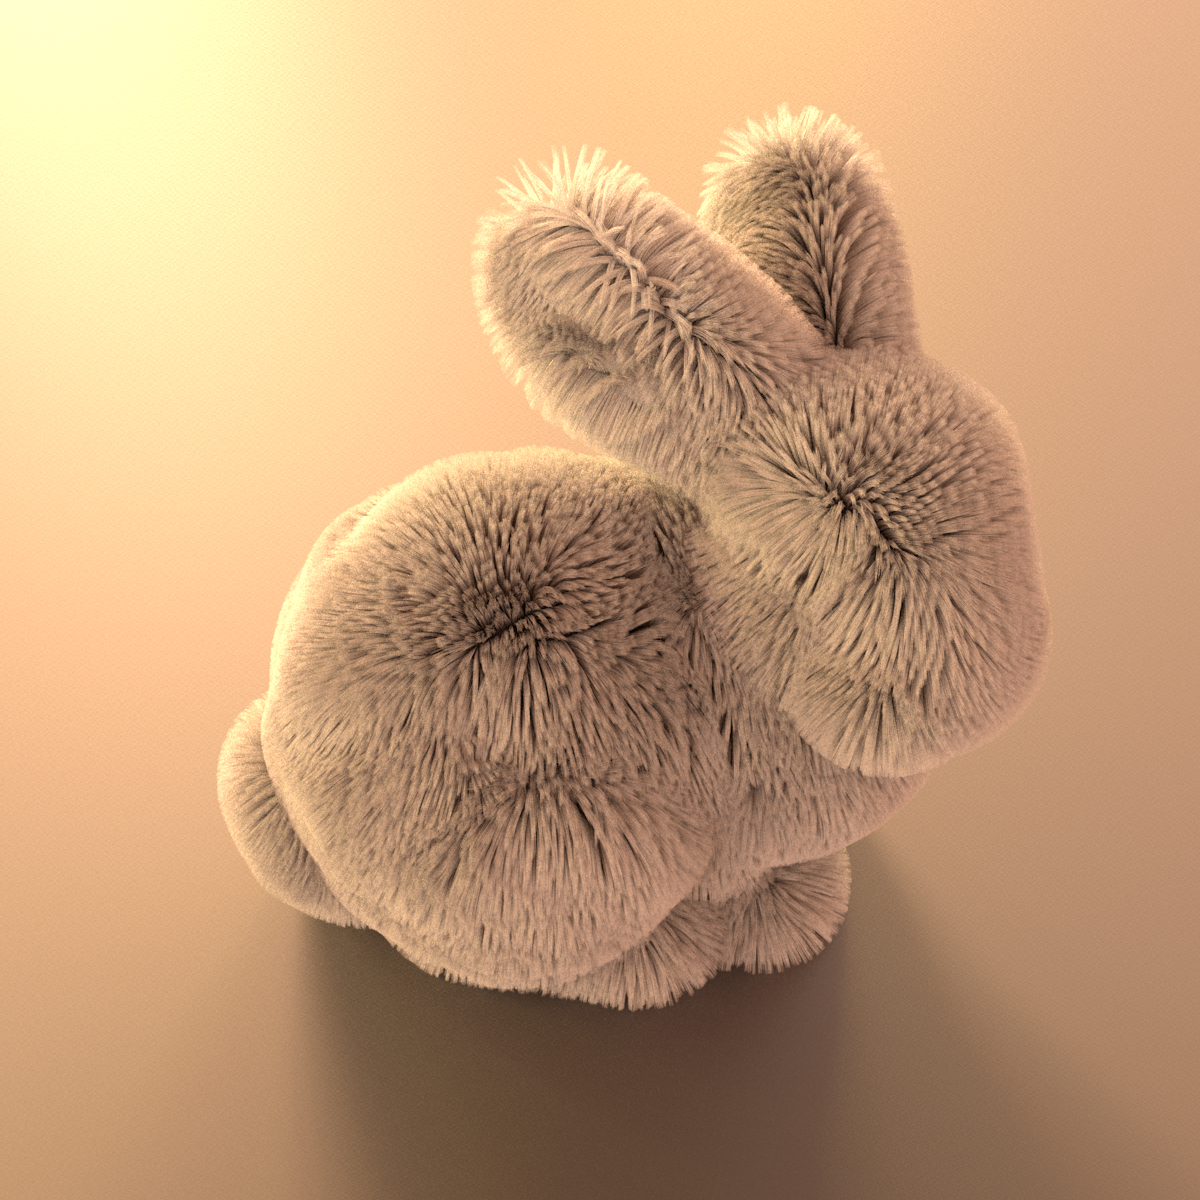
\includegraphics[width=\linewidth]{chap03/furrybunny.png}
    \caption{毛茸茸的小兔子。上百万\refvar{Curve}{}形状用于建模皮毛的小兔子模型。
        这里我们使用了不真实的长曲线来更好展示\refvar{Curve}{}的能力。}
    \label{fig:3.17}
\end{figure}
\begin{lstlisting}
`\initcode{CurveDeclarations}{=}`
class `\initvar{Curve}{}` : public `\refvar{Shape}{}` {
public:
    `\refcode{Curve Public Methods}{}`
private:
    `\refcode{Curve Private Methods}{}`
    `\refcode{Curve Private Data}{}`
};
\end{lstlisting}
\begin{lstlisting}
`\initcode{Curve Private Methods}{=}`
bool `\refvar{recursiveIntersect}{}`(const `\refvar{Ray}{}` &r, `\refvar{Float}{}` *tHit,
    `\refvar{SurfaceInteraction}{}` *isect, const `\refvar{Point3f}{}` cp[4],
    const `\refvar{Transform}{}` &rayToObject, `\refvar{Float}{}` u0, `\refvar{Float}{}` u1, int depth) const;

\end{lstlisting}

如\reffig{3.18}所示,\refvar{Curve}{}形状可以表示三种曲线。
\begin{itemize}
    \item \keyindex{平坦面}{flat}{}:这种表示的曲线总是朝向与之相交的光线;
          它们在建模细微扫掠圆柱形状如头发或皮毛时很有用。
    \item {\sffamily 圆柱}:对于在屏幕上张开几像素的曲线(如不远处看到的意大利面),
          \refvar{Curve}{}形状可以计算着色法线使得曲线看起来实际是圆柱体。
    \item \keyindex{丝带}{ribbon}{}:这个变体对于建模实际没有
          圆柱\keyindex{横截面}{cross section}{}的形状(例如一片草)很有用。
\end{itemize}
\begin{figure}[htbp]
    \centering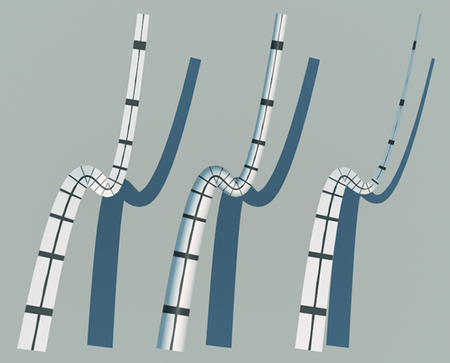
\includegraphics[width=0.5\linewidth]{chap03/threecurves.png}
    \caption{\protect\refvar{Curve}{}形状可以表示的三种曲线。
        左边是平坦曲线,总是朝向垂直于光线接近它的方向。
        中间的变体可以设置着色法线使得曲线看起来是圆柱体。
        右边是丝带,在起点和终点有固定朝向;中间的朝向在它们之间平滑插值。}
    \label{fig:3.18}
\end{figure}

枚举\refvar{CurveType}{}记录了给定的\refvar{Curve}{}实例模型是它们中的哪一个。

平坦和圆柱曲线变体旨在用于方便地近似变形的圆柱体。
要注意的是针对它们求得的相交并不对应物理可实现的3D形状,
在拿真正的圆柱体场景作参考时这可能导致微小的矛盾。
\begin{lstlisting}
`\initcode{CurveType Declarations}{=}`
enum class `\initvar{CurveType}{}` { `\initvar{Flat}{}`, `\initvar[CurveType::Cylinder]{Cylinder}{}`, `\initvar{Ribbon}{}` };
\end{lstlisting}

给定在pbrt场景描述文件中指定的曲线,
值得将其分为若干段,每段包含曲线的一部分参数$u$范围。
(这样做的一个原因是轴对齐边界框不能紧致地包围起伏的曲线,
但把贝塞尔样条分开会使其不那么弯——
多项式样条的\keyindex{变差缩减性}{variation diminishing property}{}。)
因此,\refvar{Curve}{}构造函数同时
接收$u$值的参数范围$[u_{\min},u_{\max}]$以及
指向结构体\refvar{CurveCommon}{}的指针,
它存储了控制点和各曲线段共享的关于曲线的其他信息。
这样,单个曲线段所占内存被最小化,
使得在内存中保留许多曲线更容易。
\begin{lstlisting}
`\initcode{Curve Public Methods}{=}`
`\refvar{Curve}{}`(const `\refvar{Transform}{}` *ObjectToWorld, const `\refvar{Transform}{}` *WorldToObject,
      bool reverseOrientation, const std::shared_ptr<`\refvar{CurveCommon}{}`> &common,
      `\refvar{Float}{}` uMin, `\refvar{Float}{}` uMax)
    : `\refvar{Shape}{}`(ObjectToWorld, WorldToObject, reverseOrientation),
      `\refvar{common}{}`(common), `\refvar{uMin}{}`(uMin), `\refvar{uMax}{}`(uMax) { }
\end{lstlisting}
\begin{lstlisting}
`\initcode{Curve Private Data}{=}`
const std::shared_ptr<`\refvar{CurveCommon}{}`> `\initvar{common}{}`;
const `\refvar{Float}{}` `\initvar{uMin}{}`, `\initvar{uMax}{}`; 
\end{lstlisting}

\refvar{CurveCommon}{}构造函数大多数只初始化成员变量
和传入的控制点值、曲线宽度等。
提供给它的控制点应该在曲线的物体空间内。

对于\refvar{Ribbon}{}曲线,\refvar{CurveCommon}{}存储了
曲面法线以在每个终点处让曲线定向。
构造函数预计算两个法向量的夹角并求该角正弦的倒数;
这些值会在沿曲线范围计算任意点处的朝向时很有用。
\begin{lstlisting}
`\initcode{Curve Method Definitions}{=}\initnext{CurveMethodDefinitions}`
`\refvar{CurveCommon}{}`::`\refvar{CurveCommon}{}`(const `\refvar{Point3f}{}` c[4], `\refvar{Float}{}` width0, `\refvar{Float}{}` width1,
        `\refvar{CurveType}{}` type, const `\refvar{Normal3f}{}` *norm)
    : `\refvar[CurveCommon::type]{type}{}`(type), `\refvar{cpObj}{}`{c[0], c[1], c[2], c[3]},
      `\refvar[CurveCommon::width]{width}{}`{width0, width1} {
    if (norm) {
        `\refvar[CurveCommon::n]{n}{}`[0] = `\refvar{Normalize}{}`(norm[0]);
        `\refvar[CurveCommon::n]{n}{}`[1] = `\refvar{Normalize}{}`(norm[1]);
        `\refvar{normalAngle}{}` = std::acos(`\refvar{Clamp}{}`(`\refvar{Dot}{}`(`\refvar[CurveCommon::n]{n}{}`[0], `\refvar[CurveCommon::n]{n}{}`[1]), 0, 1));
        `\refvar{invSinNormalAngle}{}` = 1 / std::sin(`\refvar{normalAngle}{}`);
    }
}
\end{lstlisting}
\begin{lstlisting}
`\initcode{CurveCommon Declarations}{=}`
struct `\initvar{CurveCommon}{}` {
    const `\refvar{CurveType}{}` `\initvar[CurveCommon::type]{type}{}`;
    const `\refvar{Point3f}{}` `\initvar{cpObj}{}`[4];
    const `\refvar{Float}{}` `\initvar[CurveCommon::width]{width}{}`[2];
    `\refvar{Normal3f}{}` `\initvar[CurveCommon::n]{n}{}`[2];
    `\refvar{Float}{}` `\initvar{normalAngle}{}`, `\initvar{invSinNormalAngle}{}`;
};
\end{lstlisting}

\refvar{Curve}{}的边界框可通过利用\keyindex{凸包性质}{convex hull property}{convex hull凸包}计算,
这是贝塞尔曲线的性质,即它们一定位于其控制点的\keyindex{凸包}{convex hull}{}内
\sidenote{译者注:在实数向量空间中,对于给定集合$X$,
所有包含$X$的凸集的交集$S$称为$X$的凸包,
它可以用$X$内所有点$(x_1,\ldots,x_n)$的线性组合来构造,
即$\displaystyle S=\{\sum\limits_{j=1}^n{t_jx_j}|x_j\in X,\sum\limits_{j=1}^n{t_j}=1,t_j\in[0,1]\}$。}。
因此,控制点的边界框给出了底层曲线的保守边界。
方法\refvar[Curve::ObjectBound]{ObjectBound}{()}首先
计算1D贝塞尔段的控制点边界框来沿曲线的中心包围样条。
然后这些边界在曲线参数范围内被展开所取最大宽度的一半,
得到\refvar{Curve}{}表示的\refvar{Shape}{}的3D边界。
\begin{lstlisting}
`\refcode{Curve Method Definitions}{+=}\lastnext{CurveMethodDefinitions}`
`\refvar{Bounds3f}{}` `\initvar{Curve::ObjectBound}{}`() const {
    `\refcode{Compute object-space control points for curve segment, cpObj}{}`
    `\refvar{Bounds3f}{}` b = `\refvar[Union2]{Union}{}`(`\refvar{Bounds3f}{}`(cpObj[0], cpObj[1]),
                       `\refvar{Bounds3f}{}`(cpObj[2], cpObj[3]));
    `\refvar{Float}{}` width[2] = { `\refvar{Lerp}{}`(`\refvar{uMin}{}`, `\refvar{common}{}`->`\refvar[CurveCommon::width]{width}{}`[0], `\refvar{common}{}`->`\refvar[CurveCommon::width]{width}{}`[1]),
                       `\refvar{Lerp}{}`(`\refvar{uMax}{}`, `\refvar{common}{}`->`\refvar[CurveCommon::width]{width}{}`[0], `\refvar{common}{}`->`\refvar[CurveCommon::width]{width}{}`[1]) };
    return `\refvar{Expand}{}`(b, std::max(width[0], width[1]) * 0.5f);
}
\end{lstlisting}

类\refvar{CurveCommon}{}存储了整条曲线的控制点,
但\refvar{Curve}{}实例通常需要对应其$u$范围的
表示贝塞尔曲线的四个控制点。
这些控制点用称为\keyindex{开花}{blossoming}{}的技术计算。
三次贝塞尔样条簇
\sidenote{译者注:原文blossom。
通过繁琐但没有技巧性的多项式代换可以证明:
对于由控制点集$A=\{\bm p_i\}_{i=0}^3$定义的
三次贝塞尔样条簇$\bm p_A(u_0,u_1,u_2)$,
其中任意截取$u_j\in[u_j^0,u_j^1],j=0,1,2$,
并设$u_j^k(i)=\left\{\begin{array}{l}
        u_j^0,\ \text{若}i<k, \\
        u_j^1,\ \text{其他},
    \end{array}\right.$
然后取新控制点集$B=\{\bm q_i\}_{i=0}^3$,
其中$\bm q_i=\bm p(u_0^3(i),u_1^2(i),u_2^1(i))$,
并设新参数变量$\displaystyle v_j=\frac{u_j-u_j^0}{u_j^1-u_j^0}$,
则有$\bm p_B(v_0,v_1,v_2)\equiv\bm p_A(u_0,u_1,u_2)$,
即实现控制点集$A$到$B$的等价变换。}
$\bm p(u_0,u_1,u_2)$由三个阶段的线性插值定义,
从原始控制点开始:
\begin{align}\label{eq:3.4}
    \bm a_i & =(1-u_0)\bm p_i+u_0\bm p_{i+1},\quad i\in[0,1,2]\nonumber\, , \\
    \bm b_j & =(1-u_1)\bm a_j+u_1\bm a_{j+1},\quad j\in[0,1]\nonumber\, ,   \\
    \bm c   & =(1-u_2)\bm b_0+u_2\bm b_1\, .
\end{align}

簇$\bm p(u,u,u)$给出了在位置$u$处的曲线值
(要自己验证的话,用$u_i=u$展开\refeq{3.4},化简,并和\refeq{3.3}比较)。

\refvar{BlossomBezier}{()}实现了该计算。
\begin{lstlisting}
`\initcode{Curve Utility Functions}{=}\initnext{CurveUtilityFunctions}`
static `\refvar{Point3f}{}` `\initvar{BlossomBezier}{}`(const `\refvar{Point3f}{}` p[4], `\refvar{Float}{}` u0, `\refvar{Float}{}` u1,
        `\refvar{Float}{}` u2) {
    `\refvar{Point3f}{}` a[3] = { `\refvar{Lerp}{}`(u0, p[0], p[1]),
                     `\refvar{Lerp}{}`(u0, p[1], p[2]),
                     `\refvar{Lerp}{}`(u0, p[2], p[3]) };
    `\refvar{Point3f}{}` b[2] = { `\refvar{Lerp}{}`(u1, a[0], a[1]), `\refvar{Lerp}{}`(u1, a[1], a[2]) };
    return `\refvar{Lerp}{}`(u2, b[0], b[1]);
}
\end{lstlisting}
\begin{figure}[htbp]
    \centering%LaTeX with PSTricks extensions
%%Creator: Inkscape 1.0.1 (3bc2e813f5, 2020-09-07)
%%Please note this file requires PSTricks extensions
\psset{xunit=.32pt,yunit=.32pt,runit=.32pt}
\begin{pspicture}(465.62508138,170.46652222)
{
\newrgbcolor{curcolor}{0 0 0}
\pscustom[linewidth=1.33333336,linecolor=curcolor]
{
\newpath
\moveto(1.60947576,70.53795366)
\curveto(154.78134799,223.70983522)(384.541779,-82.6339159)(461.13031379,147.12650044)
}
}
{
\newrgbcolor{curcolor}{0 0 0}
\pscustom[linewidth=2.66666672,linecolor=curcolor]
{
\newpath
\moveto(260.08864332,80.11087384)
\curveto(346.25011161,51.39212663)(422.83864639,32.24628627)(461.13031379,147.12650044)
}
}
{
\newrgbcolor{curcolor}{0 0 0}
\pscustom[linestyle=none,fillstyle=solid,fillcolor=curcolor]
{
\newpath
\moveto(263.62511005,79.56920716)
\curveto(263.62511005,80.52232718)(263.25011004,81.43379387)(262.5730167,82.10566055)
\curveto(261.90115002,82.78275389)(260.98968333,83.1577539)(260.03656332,83.1577539)
\curveto(259.0834433,83.1577539)(258.17197661,82.78275389)(257.50010994,82.10566055)
\curveto(256.82301659,81.43379387)(256.44801658,80.52232718)(256.44801658,79.56920716)
\curveto(256.44801658,78.61608715)(256.82301659,77.70462046)(257.50010994,77.03275378)
\curveto(258.17197661,76.35566044)(259.0834433,75.98066043)(260.03656332,75.98066043)
\curveto(260.98968333,75.98066043)(261.90115002,76.35566044)(262.5730167,77.03275378)
\curveto(263.25011004,77.70462046)(263.62511005,78.61608715)(263.62511005,79.56920716)
\closepath
\moveto(263.62511005,79.56920716)
}
}
{
\newrgbcolor{curcolor}{0 0 0}
\pscustom[linestyle=none,fillstyle=solid,fillcolor=curcolor]
{
\newpath
\moveto(350.29177836,51.56920664)
\curveto(350.29177836,52.52232665)(349.91677835,53.43379334)(349.239685,54.10566002)
\curveto(348.56781832,54.78275336)(347.65635164,55.15775337)(346.70323162,55.15775337)
\curveto(345.7501116,55.15775337)(344.83864492,54.78275336)(344.16677824,54.10566002)
\curveto(343.48968489,53.43379334)(343.11468489,52.52232665)(343.11468489,51.56920664)
\curveto(343.11468489,50.61608662)(343.48968489,49.70461993)(344.16677824,49.03275325)
\curveto(344.83864492,48.35565991)(345.7501116,47.9806599)(346.70323162,47.9806599)
\curveto(347.65635164,47.9806599)(348.56781832,48.35565991)(349.239685,49.03275325)
\curveto(349.91677835,49.70461993)(350.29177836,50.61608662)(350.29177836,51.56920664)
\closepath
\moveto(350.29177836,51.56920664)
}
}
{
\newrgbcolor{curcolor}{0 0 0}
\pscustom[linestyle=none,fillstyle=solid,fillcolor=curcolor]
{
\newpath
\moveto(426.29177979,32.90253962)
\curveto(426.29177979,33.85565963)(425.91677979,34.76712632)(425.23968644,35.438993)
\curveto(424.56781976,36.11608634)(423.65635308,36.49108635)(422.70323306,36.49108635)
\curveto(421.75011304,36.49108635)(420.83864636,36.11608634)(420.16677968,35.438993)
\curveto(419.48968633,34.76712632)(419.11468632,33.85565963)(419.11468632,32.90253962)
\curveto(419.11468632,31.9494196)(419.48968633,31.03795291)(420.16677968,30.36608623)
\curveto(420.83864636,29.68899289)(421.75011304,29.31399288)(422.70323306,29.31399288)
\curveto(423.65635308,29.31399288)(424.56781976,29.68899289)(425.23968644,30.36608623)
\curveto(425.91677979,31.03795291)(426.29177979,31.9494196)(426.29177979,32.90253962)
\closepath
\moveto(426.29177979,32.90253962)
}
}
{
\newrgbcolor{curcolor}{0 0 0}
\pscustom[linestyle=none,fillstyle=solid,fillcolor=curcolor]
{
\newpath
\moveto(464.95844719,147.56920845)
\curveto(464.95844719,148.5223338)(464.58344718,149.43379249)(463.90635384,150.10566717)
\curveto(463.23448716,150.78274984)(462.32302047,151.15774985)(461.36990046,151.15774985)
\curveto(460.41678044,151.15774985)(459.50531375,150.78274984)(458.83344708,150.10566717)
\curveto(458.15635373,149.43379249)(457.78135372,148.5223338)(457.78135372,147.56920845)
\curveto(457.78135372,146.6160831)(458.15635373,145.70462442)(458.83344708,145.03274974)
\curveto(459.50531375,144.35566706)(460.41678044,143.98066705)(461.36990046,143.98066705)
\curveto(462.32302047,143.98066705)(463.23448716,144.35566706)(463.90635384,145.03274974)
\curveto(464.58344718,145.70462442)(464.95844719,146.6160831)(464.95844719,147.56920845)
\closepath
\moveto(464.95844719,147.56920845)
}
}
{
\newrgbcolor{curcolor}{0 0 0}
\pscustom[linestyle=none,fillstyle=solid,fillcolor=curcolor]
{
\newpath
\moveto(427.14892288,154.38318208)
\curveto(427.06558955,154.00818207)(427.02392288,153.96651541)(426.98225621,153.92484874)
\curveto(426.85725621,153.88318207)(426.56558954,153.88318207)(426.31558953,153.88318207)
\curveto(425.85725619,153.88318207)(425.35725618,153.88318207)(425.35725618,153.13318206)
\curveto(425.35725618,152.84151539)(425.60725619,152.63318205)(425.89892286,152.63318205)
\curveto(426.64892287,152.63318205)(427.52392289,152.71651538)(428.31558957,152.71651538)
\curveto(429.27392292,152.71651538)(430.27392294,152.63318205)(431.19058962,152.63318205)
\curveto(431.35725629,152.63318205)(431.8572563,152.63318205)(431.8572563,153.42484873)
\curveto(431.8572563,153.88318207)(431.44058963,153.88318207)(431.19058962,153.88318207)
\curveto(430.81558962,153.88318207)(430.35725628,153.88318207)(430.02392294,153.92484874)
\lineto(431.19058962,158.54984883)
\curveto(431.56558963,158.17484882)(432.44058965,157.59151548)(433.85725634,157.59151548)
\curveto(438.48225643,157.59151548)(441.35725648,161.79984889)(441.35725648,165.42484896)
\curveto(441.35725648,168.71651569)(438.8989231,169.79984904)(436.69058973,169.79984904)
\curveto(434.81558969,169.79984904)(433.44058967,168.75818235)(433.02392299,168.38318235)
\curveto(431.98225631,169.79984904)(430.23225627,169.79984904)(429.9405896,169.79984904)
\curveto(428.98225625,169.79984904)(428.19058957,169.25818236)(427.64892289,168.29984901)
\curveto(426.98225621,167.21651566)(426.6072562,165.79984896)(426.6072562,165.67484896)
\curveto(426.6072562,165.29984896)(427.02392288,165.29984896)(427.27392288,165.29984896)
\curveto(427.56558956,165.29984896)(427.64892289,165.29984896)(427.77392289,165.42484896)
\curveto(427.85725623,165.46651562)(427.85725623,165.54984896)(428.0239229,166.21651564)
\curveto(428.52392291,168.34151568)(429.14892292,168.84151569)(429.8155896,168.84151569)
\curveto(430.10725627,168.84151569)(430.44058961,168.75818235)(430.44058961,167.88318234)
\curveto(430.44058961,167.46651566)(430.35725628,167.09151566)(430.27392294,166.71651565)
\closepath
\moveto(433.273923,167.13318232)
\curveto(434.02392301,168.04984901)(435.27392303,168.84151569)(436.56558973,168.84151569)
\curveto(438.23225642,168.84151569)(438.35725643,167.424849)(438.35725643,166.84151565)
\curveto(438.35725643,165.46651562)(437.44058974,162.1748489)(437.02392307,161.13318221)
\curveto(436.19058972,159.21651551)(434.89892303,158.54984883)(433.81558967,158.54984883)
\curveto(432.23225631,158.54984883)(431.6072563,159.79984885)(431.6072563,160.09151552)
\lineto(431.64892297,160.46651553)
\closepath
\moveto(433.273923,167.13318232)
}
}
{
\newrgbcolor{curcolor}{0 0 0}
\pscustom[linestyle=none,fillstyle=solid,fillcolor=curcolor]
{
\newpath
\moveto(446.82258862,160.0241734)
\curveto(448.28092198,160.0241734)(449.32258866,159.02417338)(449.32258866,157.02417334)
\curveto(449.32258866,154.73250663)(447.94758864,154.02417329)(446.90592195,154.02417329)
\curveto(446.15592194,154.02417329)(444.48925524,154.23250662)(443.73925523,155.35750664)
\curveto(444.61425524,155.35750664)(444.82258858,155.98250666)(444.82258858,156.39917333)
\curveto(444.82258858,156.98250668)(444.36425524,157.39917335)(443.78092189,157.39917335)
\curveto(443.28092188,157.39917335)(442.73925521,157.06584001)(442.73925521,156.31584)
\curveto(442.73925521,154.56583996)(444.65592191,153.44083994)(446.90592195,153.44083994)
\curveto(449.48925533,153.44083994)(451.28092204,155.19083997)(451.28092204,157.02417334)
\curveto(451.28092204,158.4825067)(450.11425535,159.94084006)(448.07258864,160.35750674)
\curveto(449.98925534,161.06584009)(450.69758869,162.44084011)(450.69758869,163.6075068)
\curveto(450.69758869,165.06584016)(449.03092199,166.14917352)(446.94758862,166.14917352)
\curveto(444.90592191,166.14917352)(443.32258855,165.1491735)(443.32258855,163.64917347)
\curveto(443.32258855,163.02417346)(443.73925523,162.69084012)(444.2809219,162.69084012)
\curveto(444.86425525,162.69084012)(445.23925525,163.10750679)(445.23925525,163.6075068)
\curveto(445.23925525,164.14917348)(444.86425525,164.56584015)(444.2809219,164.60750682)
\curveto(444.94758858,165.3991735)(446.19758861,165.60750684)(446.90592195,165.60750684)
\curveto(447.7392553,165.60750684)(448.90592199,165.19084016)(448.90592199,163.6075068)
\curveto(448.90592199,162.81584012)(448.65592199,161.9408401)(448.15592198,161.39917343)
\curveto(447.57258863,160.69084008)(447.03092195,160.64917341)(446.11425527,160.56584008)
\curveto(445.65592193,160.52417341)(445.61425526,160.52417341)(445.53092193,160.52417341)
\curveto(445.48925526,160.52417341)(445.32258859,160.48250674)(445.32258859,160.2741734)
\curveto(445.32258859,160.0241734)(445.48925526,160.0241734)(445.8225886,160.0241734)
\closepath
\moveto(446.82258862,160.0241734)
}
}
{
\newrgbcolor{curcolor}{0 0 0}
\pscustom[linestyle=none,fillstyle=solid,fillcolor=curcolor]
{
\newpath
\moveto(411.75142926,2.41665921)
\curveto(411.66809592,2.0416592)(411.62642925,1.99999253)(411.58476259,1.95832587)
\curveto(411.45976258,1.9166592)(411.16809591,1.9166592)(410.91809591,1.9166592)
\curveto(410.45976257,1.9166592)(409.95976256,1.9166592)(409.95976256,1.16665918)
\curveto(409.95976256,0.87499251)(410.20976256,0.66665918)(410.50142923,0.66665918)
\curveto(411.25142925,0.66665918)(412.12642926,0.74999251)(412.91809595,0.74999251)
\curveto(413.8764293,0.74999251)(414.87642932,0.66665918)(415.793096,0.66665918)
\curveto(415.95976267,0.66665918)(416.45976268,0.66665918)(416.45976268,1.45832586)
\curveto(416.45976268,1.9166592)(416.043096,1.9166592)(415.793096,1.9166592)
\curveto(415.41809599,1.9166592)(414.95976265,1.9166592)(414.62642931,1.95832587)
\lineto(415.793096,6.58332595)
\curveto(416.16809601,6.20832595)(417.04309602,5.6249926)(418.45976272,5.6249926)
\curveto(423.0847628,5.6249926)(425.95976286,9.83332602)(425.95976286,13.45832608)
\curveto(425.95976286,16.74999281)(423.50142948,17.83332617)(421.2930961,17.83332617)
\curveto(419.41809607,17.83332617)(418.04309604,16.79165948)(417.62642937,16.41665947)
\curveto(416.58476268,17.83332617)(414.83476265,17.83332617)(414.54309598,17.83332617)
\curveto(413.58476262,17.83332617)(412.79309594,17.29165949)(412.25142927,16.33332614)
\curveto(411.58476259,15.24999278)(411.20976258,13.83332609)(411.20976258,13.70832609)
\curveto(411.20976258,13.33332608)(411.62642925,13.33332608)(411.87642926,13.33332608)
\curveto(412.16809593,13.33332608)(412.25142927,13.33332608)(412.37642927,13.45832608)
\curveto(412.4597626,13.49999275)(412.4597626,13.58332609)(412.62642927,14.24999277)
\curveto(413.12642928,16.37499281)(413.75142929,16.87499282)(414.41809597,16.87499282)
\curveto(414.70976265,16.87499282)(415.04309599,16.79165948)(415.04309599,15.91665946)
\curveto(415.04309599,15.49999279)(414.95976265,15.12499278)(414.87642932,14.74999278)
\closepath
\moveto(417.87642937,15.16665945)
\curveto(418.62642939,16.08332613)(419.87642941,16.87499282)(421.1680961,16.87499282)
\curveto(422.8347628,16.87499282)(422.9597628,15.45832612)(422.9597628,14.87499278)
\curveto(422.9597628,13.49999275)(422.04309612,10.20832602)(421.62642944,9.16665934)
\curveto(420.79309609,7.24999263)(419.5014294,6.58332595)(418.41809605,6.58332595)
\curveto(416.83476269,6.58332595)(416.20976267,7.83332598)(416.20976267,8.12499265)
\lineto(416.25142934,8.49999266)
\closepath
\moveto(417.87642937,15.16665945)
}
}
{
\newrgbcolor{curcolor}{0 0 0}
\pscustom[linestyle=none,fillstyle=solid,fillcolor=curcolor]
{
\newpath
\moveto(435.71676174,5.22431714)
\lineto(435.09176173,5.22431714)
\curveto(435.05009506,4.80765046)(434.84176172,3.72431711)(434.59176172,3.55765044)
\curveto(434.46676172,3.43265044)(433.05009502,3.43265044)(432.75842835,3.43265044)
\lineto(429.34176162,3.43265044)
\curveto(431.30009499,5.1409838)(431.96676167,5.68265048)(433.05009502,6.5576505)
\curveto(434.42509505,7.64098385)(435.71676174,8.80765054)(435.71676174,10.55765057)
\curveto(435.71676174,12.80765062)(433.75842837,14.18265064)(431.38342833,14.18265064)
\curveto(429.09176162,14.18265064)(427.50842825,12.55765061)(427.50842825,10.84931725)
\curveto(427.50842825,9.93265056)(428.30009493,9.80765056)(428.50842827,9.80765056)
\curveto(428.92509495,9.80765056)(429.46676162,10.1409839)(429.46676162,10.80765058)
\curveto(429.46676162,11.14098392)(429.34176162,11.8076506)(428.38342827,11.8076506)
\curveto(428.96676161,13.09931729)(430.21676164,13.51598396)(431.09176165,13.51598396)
\curveto(432.96676169,13.51598396)(433.92509504,12.0576506)(433.92509504,10.55765057)
\curveto(433.92509504,8.93265054)(432.75842835,7.68265052)(432.17509501,7.01598384)
\lineto(427.71676159,2.55765042)
\curveto(427.50842825,2.39098375)(427.50842825,2.34931708)(427.50842825,1.84931708)
\lineto(435.17509506,1.84931708)
\closepath
\moveto(435.71676174,5.22431714)
}
}
{
\newrgbcolor{curcolor}{0 0 0}
\pscustom[linestyle=none,fillstyle=solid,fillcolor=curcolor]
{
\newpath
\moveto(334.76397447,21.83088624)
\curveto(334.68064113,21.45588624)(334.63897447,21.41421957)(334.5973078,21.3725529)
\curveto(334.4723078,21.33088623)(334.18064112,21.33088623)(333.93064112,21.33088623)
\curveto(333.47230778,21.33088623)(332.97230777,21.33088623)(332.97230777,20.58088622)
\curveto(332.97230777,20.28921955)(333.22230777,20.08088621)(333.51397444,20.08088621)
\curveto(334.26397446,20.08088621)(335.13897447,20.16421954)(335.93064116,20.16421954)
\curveto(336.88897451,20.16421954)(337.88897453,20.08088621)(338.80564121,20.08088621)
\curveto(338.97230788,20.08088621)(339.47230789,20.08088621)(339.47230789,20.87255289)
\curveto(339.47230789,21.33088623)(339.05564122,21.33088623)(338.80564121,21.33088623)
\curveto(338.4306412,21.33088623)(337.97230786,21.33088623)(337.63897452,21.3725529)
\lineto(338.80564121,25.99755299)
\curveto(339.18064122,25.62255298)(340.05564123,25.03921964)(341.47230793,25.03921964)
\curveto(346.09730802,25.03921964)(348.97230807,29.24755305)(348.97230807,32.87255312)
\curveto(348.97230807,36.16421985)(346.51397469,37.2475532)(344.30564131,37.2475532)
\curveto(342.43064128,37.2475532)(341.05564125,36.20588651)(340.63897458,35.83088651)
\curveto(339.59730789,37.2475532)(337.84730786,37.2475532)(337.55564119,37.2475532)
\curveto(336.59730784,37.2475532)(335.80564115,36.70588652)(335.26397448,35.74755317)
\curveto(334.5973078,34.66421982)(334.22230779,33.24755312)(334.22230779,33.12255312)
\curveto(334.22230779,32.74755312)(334.63897447,32.74755312)(334.88897447,32.74755312)
\curveto(335.18064114,32.74755312)(335.26397448,32.74755312)(335.38897448,32.87255312)
\curveto(335.47230781,32.91421979)(335.47230781,32.99755312)(335.63897448,33.6642198)
\curveto(336.13897449,35.78921984)(336.76397451,36.28921985)(337.43064118,36.28921985)
\curveto(337.72230786,36.28921985)(338.0556412,36.20588651)(338.0556412,35.3308865)
\curveto(338.0556412,34.91421982)(337.97230786,34.53921982)(337.88897453,34.16421981)
\closepath
\moveto(340.88897458,34.58088648)
\curveto(341.6389746,35.49755317)(342.88897462,36.28921985)(344.18064131,36.28921985)
\curveto(345.84730801,36.28921985)(345.97230801,34.87255316)(345.97230801,34.28921981)
\curveto(345.97230801,32.91421979)(345.05564133,29.62255306)(344.63897465,28.58088637)
\curveto(343.80564131,26.66421967)(342.51397461,25.99755299)(341.43064126,25.99755299)
\curveto(339.8473079,25.99755299)(339.22230789,27.24755301)(339.22230789,27.53921968)
\lineto(339.26397455,27.91421969)
\closepath
\moveto(340.88897458,34.58088648)
}
}
{
\newrgbcolor{curcolor}{0 0 0}
\pscustom[linestyle=none,fillstyle=solid,fillcolor=curcolor]
{
\newpath
\moveto(355.56264023,33.09687767)
\curveto(355.56264023,33.59687768)(355.56264023,33.59687768)(355.02097355,33.59687768)
\curveto(353.81264019,32.43021099)(352.14597349,32.43021099)(351.39597348,32.43021099)
\lineto(351.39597348,31.76354431)
\curveto(351.81264015,31.76354431)(353.06264018,31.76354431)(354.0626402,32.26354432)
\lineto(354.0626402,22.80521081)
\curveto(354.0626402,22.18021079)(354.0626402,21.93021079)(352.22930683,21.93021079)
\lineto(351.52097348,21.93021079)
\lineto(351.52097348,21.26354411)
\curveto(351.85430682,21.26354411)(354.14597353,21.34687744)(354.81264021,21.34687744)
\curveto(355.39597356,21.34687744)(357.72930693,21.26354411)(358.14597361,21.26354411)
\lineto(358.14597361,21.93021079)
\lineto(357.43764026,21.93021079)
\curveto(355.56264023,21.93021079)(355.56264023,22.18021079)(355.56264023,22.80521081)
\closepath
\moveto(355.56264023,33.09687767)
}
}
{
\newrgbcolor{curcolor}{0 0 0}
\pscustom[linestyle=none,fillstyle=solid,fillcolor=curcolor]
{
\newpath
\moveto(247.06522653,44.59239334)
\curveto(246.98189319,44.21739333)(246.94022653,44.17572666)(246.89855986,44.13406)
\curveto(246.77355986,44.09239333)(246.48189319,44.09239333)(246.23189318,44.09239333)
\curveto(245.77355984,44.09239333)(245.27355983,44.09239333)(245.27355983,43.34239332)
\curveto(245.27355983,43.05072664)(245.52355983,42.84239331)(245.81522651,42.84239331)
\curveto(246.56522652,42.84239331)(247.44022654,42.92572664)(248.23189322,42.92572664)
\curveto(249.19022657,42.92572664)(250.19022659,42.84239331)(251.10689327,42.84239331)
\curveto(251.27355994,42.84239331)(251.77355995,42.84239331)(251.77355995,43.63405999)
\curveto(251.77355995,44.09239333)(251.35689328,44.09239333)(251.10689327,44.09239333)
\curveto(250.73189327,44.09239333)(250.27355992,44.09239333)(249.94022658,44.13406)
\lineto(251.10689327,48.75906008)
\curveto(251.48189328,48.38406008)(252.3568933,47.80072673)(253.77355999,47.80072673)
\curveto(258.39856008,47.80072673)(261.27356013,52.00906015)(261.27356013,55.63406021)
\curveto(261.27356013,58.92572694)(258.81522675,60.0090603)(256.60689338,60.0090603)
\curveto(254.73189334,60.0090603)(253.35689332,58.96739361)(252.94022664,58.5923936)
\curveto(251.89855995,60.0090603)(250.14855992,60.0090603)(249.85689325,60.0090603)
\curveto(248.8985599,60.0090603)(248.10689322,59.46739362)(247.56522654,58.50906027)
\curveto(246.89855986,57.42572692)(246.52355985,56.00906022)(246.52355985,55.88406022)
\curveto(246.52355985,55.50906021)(246.94022653,55.50906021)(247.19022653,55.50906021)
\curveto(247.4818932,55.50906021)(247.56522654,55.50906021)(247.69022654,55.63406021)
\curveto(247.77355988,55.67572688)(247.77355988,55.75906022)(247.94022655,56.4257269)
\curveto(248.44022656,58.55072694)(249.06522657,59.05072695)(249.73189325,59.05072695)
\curveto(250.02355992,59.05072695)(250.35689326,58.96739361)(250.35689326,58.09239359)
\curveto(250.35689326,57.67572692)(250.27355992,57.30072691)(250.19022659,56.92572691)
\closepath
\moveto(253.19022665,57.34239358)
\curveto(253.94022666,58.25906026)(255.19022668,59.05072695)(256.48189337,59.05072695)
\curveto(258.14856007,59.05072695)(258.27356007,57.63406025)(258.27356007,57.05072691)
\curveto(258.27356007,55.67572688)(257.35689339,52.38406015)(256.94022672,51.34239347)
\curveto(256.10689337,49.42572676)(254.81522668,48.75906008)(253.73189332,48.75906008)
\curveto(252.14855996,48.75906008)(251.52355995,50.00906011)(251.52355995,50.30072678)
\lineto(251.56522661,50.67572679)
\closepath
\moveto(253.19022665,57.34239358)
}
}
{
\newrgbcolor{curcolor}{0 0 0}
\pscustom[linestyle=none,fillstyle=solid,fillcolor=curcolor]
{
\newpath
\moveto(271.23889235,49.94171798)
\curveto(271.23889235,51.98338469)(270.98889235,53.48338472)(270.155559,54.77505141)
\curveto(269.57222565,55.60838476)(268.40555896,56.35838477)(266.9472256,56.35838477)
\curveto(262.61389219,56.35838477)(262.61389219,51.27505134)(262.61389219,49.94171798)
\curveto(262.61389219,48.60838463)(262.61389219,43.6500512)(266.9472256,43.6500512)
\curveto(271.23889235,43.6500512)(271.23889235,48.60838463)(271.23889235,49.94171798)
\closepath
\moveto(266.9472256,44.19171788)
\curveto(266.07222559,44.19171788)(264.94722557,44.69171789)(264.57222556,46.19171791)
\curveto(264.32222555,47.27505127)(264.32222555,48.81671796)(264.32222555,50.19171799)
\curveto(264.32222555,51.56671802)(264.32222555,52.98338471)(264.57222556,53.98338473)
\curveto(264.98889223,55.44171809)(266.15555892,55.85838476)(266.9472256,55.85838476)
\curveto(267.94722562,55.85838476)(268.90555897,55.23338475)(269.23889231,54.1500514)
\curveto(269.53055899,53.15005138)(269.57222565,51.81671802)(269.57222565,50.19171799)
\curveto(269.57222565,48.81671796)(269.57222565,47.44171794)(269.32222565,46.27505125)
\curveto(268.94722564,44.56671788)(267.69722562,44.19171788)(266.9472256,44.19171788)
\closepath
\moveto(266.9472256,44.19171788)
}
}
\end{pspicture}

    \caption{一段贝塞尔曲线开花求控制点。
        \protect\refeq{3.5}中四簇给出从$u_{\min}$到$u_{\max}$的曲线控制点。
        开花提供了优雅方法计算整条曲线的子集曲线的贝塞尔控制点。}
    \label{fig:3.19}
\end{figure}

范围从$u_{\min}$到$u_{\max}$的曲线段的四个控制点由簇给出(\reffig{3.19}):
\begin{align}\label{eq:3.5}
    \bm p_0 & =\bm p(u_{\min},u_{\min},u_{\min})\nonumber\, , \\
    \bm p_1 & =\bm p(u_{\min},u_{\min},u_{\max})\nonumber\, , \\
    \bm p_2 & =\bm p(u_{\min},u_{\max},u_{\max})\nonumber\, , \\
    \bm p_3 & =\bm p(u_{\max},u_{\max},u_{\max})\, .
\end{align}

有了该机制,计算\refvar{Curve}{}负责的曲线段的四个控制点很简单。
\begin{lstlisting}
`\initcode{Compute object-space control points for curve segment, cpObj}{=}`
`\refvar{Point3f}{}` cpObj[4];
cpObj[0] = `\refvar{BlossomBezier}{}`(`\refvar{common}{}`->`\refvar{cpObj}{}`, `\refvar{uMin}{}`, `\refvar{uMin}{}`, `\refvar{uMin}{}`);
cpObj[1] = `\refvar{BlossomBezier}{}`(`\refvar{common}{}`->`\refvar{cpObj}{}`, `\refvar{uMin}{}`, `\refvar{uMin}{}`, `\refvar{uMax}{}`);
cpObj[2] = `\refvar{BlossomBezier}{}`(`\refvar{common}{}`->`\refvar{cpObj}{}`, `\refvar{uMin}{}`, `\refvar{uMax}{}`, `\refvar{uMax}{}`);
cpObj[3] = `\refvar{BlossomBezier}{}`(`\refvar{common}{}`->`\refvar{cpObj}{}`, `\refvar{uMax}{}`, `\refvar{uMax}{}`, `\refvar{uMax}{}`);
\end{lstlisting}

\refvar{Curve}{}相交算法基于尽快抛弃可以确定一定不会与光线相交的曲线段,
否则就递归地将曲线对半分为更小的两个曲线段然后再测试。
最终,曲线被线性近似以进行高效相交测试。
在一些准备工作后,\refvar{recursiveIntersect}{()}调用
使用\refvar{Curve}{}表示的整段曲线启动该进程。
\begin{lstlisting}
`\refcode{Curve Method Definitions}{+=}\lastnext{CurveMethodDefinitions}`
bool `\refvar{Curve}{}`::`\initvar[Curve::Intersect]{\refvar[Shape::Intersect]{Intersect}{}}{}`(const `\refvar{Ray}{}` &r, `\refvar{Float}{}` *tHit,
        `\refvar{SurfaceInteraction}{}` *isect, bool testAlphaTexture) const {
    `\refcode{Transform Ray to object space}{}`
    `\refcode{Compute object-space control points for curve segment, cpObj}{}`
    `\refcode{Project curve control points to plane perpendicular to ray}{}`
    `\refcode{Compute refinement depth for curve, maxDepth}{}`
    return `\refvar{recursiveIntersect}{}`(ray, tHit, isect, cp, `\refvar[Transform::Inverse]{Inverse}{}`(objectToRay),
                              `\refvar{uMin}{}`, `\refvar{uMax}{}`, maxDepth);
}
\end{lstlisting}

如同\refsub{三角形相交}的光线-三角形相交算法,
光线-曲线相交测试基于把曲线变换到射线端点在原点、
射线方向对齐$+z$轴的坐标系。
一开始就执行该变换极大减少了相交测试必须执行的运算量。

对于\refvar{Curve}{}形状,我们需要变换的显式表示,
所以这里用函数\refvar{LookAt}{()}来生成它。
原点是射线的端点,“注视”点是从原点沿射线方向偏移的点,
“向上”方向是正交于射线方向的任意方向。
\begin{lstlisting}
`\initcode{Project curve control points to plane perpendicular to ray}{=}`
`\refvar{Vector3f}{}` dx, dy;
`\refvar{CoordinateSystem}{}`(ray.`\refvar[Ray::d]{d}{}`, &dx, &dy);
`\refvar{Transform}{}` objectToRay = `\refvar{LookAt}{}`(ray.`\refvar[Ray::o]{o}{}`, ray.`\refvar[Ray::o]{o}{}` + ray.`\refvar[Ray::d]{d}{}`, dx);
`\refvar{Point3f}{}` cp[4] = { objectToRay(cpObj[0]), objectToRay(cpObj[1]),
                  objectToRay(cpObj[2]), objectToRay(cpObj[3]) };
\end{lstlisting}

计算细分曲线的最大次数,这样与最精细级别的最终线性化曲线的距离
就被限定在小于某微小固定的距离内。
我们不深入该计算的细节
\sidenote{译者注:我对这段代码的理解是:
通过比较{\ttfamily cp[1]}与{\ttfamily cp[0]、cp[2]}的中点之差以及
{\ttfamily cp[2]}与{\ttfamily cp[1]、cp[3]}的中点之差,并取全部维度的最大绝对值,
{\ttfamily L0}表示了曲线的弯曲程度;{\ttfamily eps}表示最大宽度的一半。
{\ttfamily L0}与{\ttfamily eps}的比值反映了相应精度要求,
取对数后对应最大划分次数。},
它在代码片\refcode{Compute refinement depth for curve, maxDepth}{}中实现。
\begin{lstlisting}
`\initcode{Compute refinement depth for curve, maxDepth}{=}`
`\refvar{Float}{}` L0 = 0;
for (int i = 0; i < 2; ++i)
    L0 = std::max(L0,
         std::max(std::max(std::abs(cp[i].x - 2 * cp[i + 1].x + cp[i + 2].x),
                           std::abs(cp[i].y - 2 * cp[i + 1].y + cp[i + 2].y)),
                  std::abs(cp[i].z - 2 * cp[i + 1].z + cp[i + 2].z)));
`\refvar{Float}{}` eps = std::max(`\refvar{common}{}`->`\refvar[CurveCommon::width]{width}{}`[0], `\refvar{common}{}`->`\refvar[CurveCommon::width]{width}{}`[1]) * .05f; // width / 20
#define LOG4(x) (std::log(x) * 0.7213475108f)
`\refvar{Float}{}` fr0 = LOG4(1.41421356237f * 12.f * L0 / (8.f * eps));
#undef LOG4
int r0 = (int)std::round(fr0);
int maxDepth = `\refvar{Clamp}{}`(r0, 0, 10);
\end{lstlisting}

然后方法\refvar{recursiveIntersect}{()}测试给定射线是否与
在给定参数范围{\ttfamily [u0,u1]}内的曲线段相交。
\begin{lstlisting}
`\refcode{Curve Method Definitions}{+=}\lastcode{CurveMethodDefinitions}`
bool `\refvar{Curve}{}`::`\initvar{recursiveIntersect}{}`(const `\refvar{Ray}{}` &ray, `\refvar{Float}{}` *tHit,
        `\refvar{SurfaceInteraction}{}` *isect, const `\refvar{Point3f}{}` cp[4],
        const `\refvar{Transform}{}` &rayToObject, `\refvar{Float}{}` u0, `\refvar{Float}{}` u1,
        int depth) const {
    `\refcode{Try to cull curve segment versus ray}{}`
    if (depth > 0) {
        `\refcode{Split curve segment into sub-segments and test for intersection}{}`
    } else {
        `\refcode{Intersect ray with curve segment}{}`
    }
}
\end{lstlisting}

该方法先开始检查射线是否与曲线段的边界框相交;
如果没有,则不可能相交,它就立即返回。
\begin{lstlisting}
`\initcode{Try to cull curve segment versus ray}{=}`
`\refcode{Compute bounding box of curve segment, curveBounds}{}`
`\refcode{Compute bounding box of ray, rayBounds}{}`
if (`\refvar{Overlaps}{}`(curveBounds, rayBounds) == false)
    return false;
\end{lstlisting}

沿着\refvar{Curve::ObjectBound}{()}的实现路线,
可以通过接收曲线控制点的边界并在曲线考虑的$u$范围内
展开最大宽度的一半来求得该段的保守边界框。
\begin{lstlisting}
`\initcode{Compute bounding box of curve segment, curveBounds}{=}`
`\refvar{Bounds3f}{}` curveBounds =
    `\refvar[Union2]{Union}{}`(`\refvar{Bounds3f}{}`(cp[0], cp[1]), `\refvar{Bounds3f}{}`(cp[2], cp[3]));
`\refvar{Float}{}` maxWidth = std::max(`\refvar{Lerp}{}`(u0, `\refvar{common}{}`->`\refvar[CurveCommon::width]{width}{}`[0], `\refvar{common}{}`->`\refvar[CurveCommon::width]{width}{}`[1]),
                          `\refvar{Lerp}{}`(u1, `\refvar{common}{}`->`\refvar[CurveCommon::width]{width}{}`[0], `\refvar{common}{}`->`\refvar[CurveCommon::width]{width}{}`[1]));
curveBounds = `\refvar{Expand}{}`(curveBounds, 0.5 * maxWidth);
\end{lstlisting}

因为在相交空间内射线端点在$(0,0,0)$且其方向对齐$+z$轴,
所以其边界框只包含$x$和$y$原点(\reffig{3.20});
其$z$范围由参数范围覆盖的相应部分给出。
\begin{figure}[htbp]
    \centering%LaTeX with PSTricks extensions
%%Creator: Inkscape 1.0.1 (3bc2e813f5, 2020-09-07)
%%Please note this file requires PSTricks extensions
\psset{xunit=.5pt,yunit=.5pt,runit=.5pt}
\begin{pspicture}(480,186.66666667)
{
\newrgbcolor{curcolor}{0 0 0}
\pscustom[linestyle=none,fillstyle=solid,fillcolor=curcolor]
{
\newpath
\moveto(107.36460514,22.96364116)
\lineto(106.02085579,22.96364116)
\curveto(105.46356378,23.6719745)(104.95835444,24.42197451)(104.50523044,25.20843319)
\curveto(104.0521051,25.99489054)(103.66147976,26.81259988)(103.33335442,27.66155723)
\curveto(103.00523042,28.5105159)(102.75523041,29.37509992)(102.57814641,30.26572526)
\curveto(102.40106374,31.15634927)(102.31252241,32.05218262)(102.31252241,32.9636413)
\curveto(102.31252241,33.88551598)(102.40106374,34.79176666)(102.58335441,35.67718267)
\curveto(102.76564641,36.56260001)(103.01564642,37.42718269)(103.34377175,38.26572537)
\curveto(103.67189709,39.10426671)(104.06252243,39.92197473)(104.51564644,40.7084334)
\curveto(104.96877178,41.49489075)(105.47397978,42.25010009)(106.02085579,42.97405877)
\lineto(107.36460514,42.97405877)
\curveto(106.86981313,42.16676676)(106.43231313,41.37510008)(106.04168779,40.5938494)
\curveto(105.65106378,39.81260006)(105.32814645,39.01572538)(105.06252244,38.20843337)
\curveto(104.79689711,37.40114136)(104.59897977,36.56780801)(104.45835443,35.70843334)
\curveto(104.31773043,34.84905866)(104.2500211,33.94280798)(104.2500211,32.98447463)
\curveto(104.2500211,32.09384929)(104.32293843,31.21364127)(104.47397977,30.33864126)
\curveto(104.6250211,29.46364125)(104.83335444,28.60426657)(105.10418911,27.76051589)
\curveto(105.37502111,26.91676655)(105.70314645,26.0938492)(106.08335446,25.29176653)
\curveto(106.4635638,24.48968252)(106.89064647,23.71364117)(107.36460514,22.96364116)
\closepath
\moveto(107.36460514,22.96364116)
}
}
{
\newrgbcolor{curcolor}{0 0 0}
\pscustom[linestyle=none,fillstyle=solid,fillcolor=curcolor]
{
\newpath
\moveto(108.58335449,34.97405866)
\curveto(108.58335449,36.78134935)(108.77085583,38.2344747)(109.1406465,39.33343338)
\curveto(109.5104385,40.43239207)(110.06252251,41.28134941)(110.79689719,41.88030809)
\curveto(111.53127186,42.47926676)(112.45314654,42.77614143)(113.56252256,42.77614143)
\curveto(114.38023057,42.77614143)(115.09897991,42.60947476)(115.71877192,42.28134942)
\curveto(116.33856393,41.95322409)(116.84897994,41.47405875)(117.25002128,40.85426674)
\curveto(117.65106395,40.23447473)(117.96877195,39.47405872)(118.19793862,38.58343337)
\curveto(118.42710529,37.69280803)(118.54168796,36.48968268)(118.54168796,34.97405866)
\curveto(118.54168796,33.18239197)(118.35939729,31.73447461)(117.98960529,30.63551593)
\curveto(117.61981328,29.53655725)(117.07293861,28.68239191)(116.33856393,28.08343323)
\curveto(115.60418925,27.48447456)(114.68231324,27.18239189)(113.56252256,27.18239189)
\curveto(112.08856387,27.18239189)(110.93231319,27.70843323)(110.09377184,28.76572524)
\curveto(109.08856383,30.03655726)(108.58335449,32.10426662)(108.58335449,34.97405866)
\closepath
\moveto(110.51043852,34.97405866)
\curveto(110.51043852,32.46884929)(110.80210519,30.7969746)(111.39064653,29.96884926)
\curveto(111.9791892,29.14072525)(112.70314655,28.72405857)(113.56252256,28.72405857)
\curveto(114.42189724,28.72405857)(115.14585591,29.14072525)(115.73439726,29.97405859)
\curveto(116.3229386,30.80739194)(116.61460527,32.47405862)(116.61460527,34.97405866)
\curveto(116.61460527,37.48968269)(116.3229386,39.15634938)(115.73439726,39.98447473)
\curveto(115.14585591,40.81260007)(114.4166879,41.22405874)(113.54168789,41.22405874)
\curveto(112.68231321,41.22405874)(111.9948132,40.85947474)(111.4791892,40.13030806)
\curveto(110.83335452,39.19801605)(110.51043852,37.47926669)(110.51043852,34.97405866)
\closepath
\moveto(110.51043852,34.97405866)
}
}
{
\newrgbcolor{curcolor}{0 0 0}
\pscustom[linestyle=none,fillstyle=solid,fillcolor=curcolor]
{
\newpath
\moveto(121.593772,27.44280789)
\lineto(121.593772,29.57822392)
\lineto(123.72918936,29.57822392)
\lineto(123.72918936,27.44280789)
\curveto(123.72918936,26.65634921)(123.58856403,26.0261412)(123.31252269,25.54176653)
\curveto(123.03648002,25.05739186)(122.59377202,24.68759985)(121.98960534,24.42197451)
\lineto(121.468772,25.22405853)
\curveto(121.86460534,25.39593319)(122.15627201,25.6511412)(122.34377201,25.98968254)
\curveto(122.53127201,26.32822387)(122.63543868,26.81259988)(122.65627202,27.44280789)
\closepath
\moveto(121.593772,27.44280789)
}
}
{
\newrgbcolor{curcolor}{0 0 0}
\pscustom[linestyle=none,fillstyle=solid,fillcolor=curcolor]
{
\newpath
\moveto(125.91668806,34.97405866)
\curveto(125.91668806,36.78134935)(126.1041894,38.2344747)(126.47398007,39.33343338)
\curveto(126.84377207,40.43239207)(127.39585608,41.28134941)(128.13023076,41.88030809)
\curveto(128.86460543,42.47926676)(129.78648011,42.77614143)(130.89585613,42.77614143)
\curveto(131.71356414,42.77614143)(132.43231348,42.60947476)(133.05210549,42.28134942)
\curveto(133.6718975,41.95322409)(134.18231351,41.47405875)(134.58335485,40.85426674)
\curveto(134.98439752,40.23447473)(135.30210552,39.47405872)(135.53127219,38.58343337)
\curveto(135.76043886,37.69280803)(135.87502153,36.48968268)(135.87502153,34.97405866)
\curveto(135.87502153,33.18239197)(135.69273086,31.73447461)(135.32293886,30.63551593)
\curveto(134.95314685,29.53655725)(134.40627218,28.68239191)(133.6718975,28.08343323)
\curveto(132.93752282,27.48447456)(132.01564681,27.18239189)(130.89585613,27.18239189)
\curveto(129.42189744,27.18239189)(128.26564676,27.70843323)(127.42710541,28.76572524)
\curveto(126.4218974,30.03655726)(125.91668806,32.10426662)(125.91668806,34.97405866)
\closepath
\moveto(127.84377209,34.97405866)
\curveto(127.84377209,32.46884929)(128.13543876,30.7969746)(128.7239801,29.96884926)
\curveto(129.31252277,29.14072525)(130.03648012,28.72405857)(130.89585613,28.72405857)
\curveto(131.75523081,28.72405857)(132.47918948,29.14072525)(133.06773082,29.97405859)
\curveto(133.65627217,30.80739194)(133.94793884,32.47405862)(133.94793884,34.97405866)
\curveto(133.94793884,37.48968269)(133.65627217,39.15634938)(133.06773082,39.98447473)
\curveto(132.47918948,40.81260007)(131.75002147,41.22405874)(130.87502146,41.22405874)
\curveto(130.01564678,41.22405874)(129.32814677,40.85947474)(128.81252277,40.13030806)
\curveto(128.16668809,39.19801605)(127.84377209,37.47926669)(127.84377209,34.97405866)
\closepath
\moveto(127.84377209,34.97405866)
}
}
{
\newrgbcolor{curcolor}{0 0 0}
\pscustom[linestyle=none,fillstyle=solid,fillcolor=curcolor]
{
\newpath
\moveto(142.85418962,32.9636413)
\curveto(142.85418962,32.04697462)(142.76564696,31.14593327)(142.58335495,30.26051593)
\curveto(142.40106429,29.37509992)(142.15106428,28.5105159)(141.82293894,27.67197456)
\curveto(141.49481361,26.83343321)(141.1041896,26.0157252)(140.65106426,25.22926653)
\curveto(140.19793892,24.44280785)(139.69273091,23.68759984)(139.14585624,22.96364116)
\lineto(137.80210556,22.96364116)
\curveto(138.28648023,23.75530784)(138.72398024,24.54176652)(139.11460557,25.32822386)
\curveto(139.50523091,26.11468254)(139.82814692,26.91155722)(140.09377225,27.72405856)
\curveto(140.35939759,28.53655724)(140.56252293,29.37509992)(140.70314693,30.23447459)
\curveto(140.84377226,31.09384927)(140.91668826,32.00009995)(140.91668826,32.94280796)
\curveto(140.91668826,33.83343331)(140.84377226,34.71364132)(140.69273093,35.58864133)
\curveto(140.54168826,36.46364135)(140.33335492,37.32301602)(140.06252292,38.1667667)
\curveto(139.79168825,39.01051605)(139.46356425,39.83343339)(139.07814691,40.6407254)
\curveto(138.6927309,41.44801608)(138.2656469,42.22405876)(137.80210556,42.97405877)
\lineto(139.14585624,42.97405877)
\curveto(139.70314692,42.26572542)(140.20835492,41.51572541)(140.66668826,40.72926674)
\curveto(141.1250216,39.94280806)(141.51564694,39.11989072)(141.83856428,38.27093337)
\curveto(142.16148028,37.42197469)(142.41148029,36.54697468)(142.58856429,35.65634933)
\curveto(142.76564696,34.76572532)(142.85418962,33.86468264)(142.85418962,32.9636413)
\closepath
\moveto(142.85418962,32.9636413)
}
}
{
\newrgbcolor{curcolor}{0 0 0}
\pscustom[linewidth=1.33333335,linecolor=curcolor]
{
\newpath
\moveto(93.12500127,10.3802056)
\lineto(93.12500127,177.47395854)
}
}
{
\newrgbcolor{curcolor}{0 0 0}
\pscustom[linewidth=1.33333335,linecolor=curcolor]
{
\newpath
\moveto(9.57291746,52.1510395)
\lineto(469.09375572,52.1510395)
}
}
{
\newrgbcolor{curcolor}{0 0 0}
\pscustom[linestyle=none,fillstyle=solid,fillcolor=curcolor]
{
\newpath
\moveto(98.00000134,51.99999817)
\curveto(98.00000134,53.23958218)(97.51041733,54.42708087)(96.63541732,55.30208088)
\curveto(95.7604173,56.17708089)(94.57291862,56.6666649)(93.3333346,56.6666649)
\curveto(92.09375059,56.6666649)(90.90625191,56.17708089)(90.03125189,55.30208088)
\curveto(89.15625188,54.42708087)(88.66666787,53.23958218)(88.66666787,51.99999817)
\curveto(88.66666787,50.76041415)(89.15625188,49.57291547)(90.03125189,48.69791545)
\curveto(90.90625191,47.82291544)(92.09375059,47.33333144)(93.3333346,47.33333144)
\curveto(94.57291862,47.33333144)(95.7604173,47.82291544)(96.63541732,48.69791545)
\curveto(97.51041733,49.57291547)(98.00000134,50.76041415)(98.00000134,51.99999817)
\closepath
\moveto(98.00000134,51.99999817)
}
}
{
\newrgbcolor{curcolor}{0.36078432 0.49803922 0.7019608}
\pscustom[linewidth=2.13333339,linecolor=curcolor]
{
\newpath
\moveto(149.66666871,123.1718738)
\lineto(149.74479404,123.24479114)
\lineto(149.81771004,123.32291647)
\lineto(149.97396071,123.47395781)
\lineto(150.28125271,123.78124981)
\lineto(150.90104339,124.38020715)
\lineto(152.14062741,125.55729117)
\lineto(154.63541811,127.80208186)
\lineto(160.11979418,132.20312459)
\lineto(165.33333559,135.74999931)
\lineto(165.41666892,135.79687397)
\lineto(165.49479425,135.84895797)
\lineto(165.97916893,136.14583265)
\lineto(166.62500227,136.53645798)
\lineto(167.92187695,137.29687399)
\lineto(170.52604366,138.72395801)
\lineto(170.70312766,138.81770735)
\lineto(170.88021033,138.90625002)
\lineto(171.234377,139.08854069)
\lineto(171.94791968,139.44791669)
\lineto(173.36979436,140.1406247)
\lineto(176.23437707,141.41666605)
\lineto(176.32291974,141.45312472)
\lineto(176.40625307,141.48958338)
\lineto(176.57291974,141.55729139)
\lineto(176.90625308,141.69791672)
\lineto(177.58333575,141.96874872)
\lineto(178.9270851,142.4947914)
\lineto(179.01562777,142.52604073)
\lineto(179.26562778,142.6197914)
\lineto(179.60416911,142.7447914)
\lineto(180.28125312,142.9895834)
\lineto(181.63541847,143.45833274)
\lineto(181.82291981,143.52083275)
\lineto(182.00521048,143.58333275)
\lineto(182.37500248,143.70312475)
\lineto(183.10937716,143.93749942)
\lineto(184.58854385,144.38541542)
\lineto(184.77604385,144.43749942)
\lineto(184.95833585,144.49479143)
\lineto(185.33333586,144.59895809)
\lineto(186.07291987,144.8020821)
\lineto(187.56250256,145.18749943)
\lineto(187.65104389,145.20833277)
\lineto(187.74479456,145.2343741)
\lineto(187.92708523,145.27604077)
\lineto(188.29166923,145.36458344)
\lineto(189.02604391,145.53645811)
\lineto(190.4947946,145.85937411)
\lineto(190.58333593,145.88020744)
\lineto(190.67708526,145.89583278)
\lineto(190.85937727,145.93749945)
\lineto(191.22916927,146.01041545)
\lineto(191.96354395,146.15625011)
\lineto(193.43750264,146.42187412)
\lineto(193.52604397,146.43749945)
\lineto(193.6093773,146.44791679)
\lineto(193.78125331,146.47916612)
\lineto(194.13021064,146.53645812)
\lineto(194.81771065,146.64583279)
\lineto(194.90625332,146.66145812)
\lineto(194.98958666,146.67187412)
\lineto(195.16146133,146.69791679)
\lineto(195.51041866,146.74999946)
\lineto(196.20312801,146.84895812)
\lineto(196.28646134,146.85937412)
\lineto(196.37500268,146.86979146)
\lineto(196.54687734,146.89583279)
\lineto(196.89062802,146.94270746)
\lineto(197.58333603,147.02604079)
\lineto(198.97396138,147.18749946)
\lineto(199.06771071,147.19270746)
\lineto(199.34896138,147.22395813)
\lineto(199.72916939,147.26041546)
\lineto(200.4791694,147.3333328)
\lineto(200.57812807,147.3385408)
\lineto(200.6718774,147.34895813)
\lineto(201.23437741,147.3958328)
\lineto(201.99479475,147.4531248)
\lineto(202.08854409,147.4583328)
\lineto(202.18229475,147.4687488)
\lineto(202.36979476,147.47916613)
\lineto(202.75000276,147.50520747)
\lineto(202.93750276,147.5156248)
\lineto(203.13021077,147.5260408)
\lineto(203.50521077,147.54687413)
\lineto(203.59896144,147.55729147)
\lineto(203.69792011,147.55729147)
\lineto(203.88541878,147.56770747)
\lineto(204.26562812,147.5885408)
\lineto(204.45312812,147.59895813)
\lineto(204.64583612,147.60416613)
\lineto(205.02604413,147.61979147)
\lineto(205.20312813,147.63020747)
\lineto(205.73437747,147.6458328)
\lineto(205.82292014,147.6510408)
\lineto(205.91146147,147.6510408)
\lineto(206.44271081,147.66666614)
\lineto(206.53125348,147.67187414)
\lineto(206.61979481,147.67187414)
\lineto(206.79687748,147.67708214)
\lineto(206.88541882,147.67708214)
\lineto(206.97396149,147.68229147)
\lineto(207.15104416,147.68229147)
\lineto(207.23958682,147.68749947)
\lineto(207.50521083,147.68749947)
\lineto(207.59896149,147.69270747)
\lineto(207.86458683,147.69270747)
\lineto(207.95312817,147.6979168)
\lineto(208.57292017,147.6979168)
\lineto(208.66146151,147.7031248)
\lineto(209.46354419,147.7031248)
\lineto(209.55208552,147.6979168)
\lineto(210.17708553,147.6979168)
\lineto(210.2656282,147.69270747)
\lineto(210.53125353,147.69270747)
\lineto(210.7135442,147.68749947)
\lineto(210.88541887,147.68749947)
\lineto(211.06250288,147.68229147)
\lineto(211.14583621,147.68229147)
\lineto(211.23437754,147.67708214)
\lineto(211.41146155,147.67708214)
\lineto(211.50000288,147.67187414)
\lineto(211.58333622,147.67187414)
\lineto(211.76041889,147.66666614)
\lineto(212.10937756,147.65625014)
\lineto(212.19792022,147.65625014)
\lineto(212.28646156,147.6510408)
\lineto(212.45833623,147.6458328)
\lineto(212.8125029,147.63541547)
\lineto(212.89583623,147.63020747)
\lineto(212.98437757,147.63020747)
\lineto(213.16146157,147.61979147)
\lineto(213.51041891,147.60937413)
\lineto(213.68750291,147.59895813)
\lineto(213.85937758,147.5937488)
\lineto(214.21354425,147.5781248)
\lineto(214.91146159,147.54166613)
\lineto(215.26562827,147.5208328)
\lineto(215.61458694,147.49999947)
\lineto(216.31771095,147.4583328)
\lineto(216.41146162,147.4531248)
\lineto(216.51041895,147.4479168)
\lineto(216.69792029,147.43229147)
\lineto(217.08333629,147.40625013)
\lineto(217.8437523,147.34895813)
\lineto(217.93750297,147.3437488)
\lineto(218.03646164,147.3333328)
\lineto(218.22396164,147.31770746)
\lineto(218.60937764,147.28645813)
\lineto(219.36979499,147.2187488)
\lineto(219.46875232,147.2135408)
\lineto(219.56250299,147.2031248)
\lineto(219.75521099,147.18229146)
\lineto(220.135419,147.15104079)
\lineto(220.90104434,147.07291679)
\lineto(222.43229503,146.90625012)
\lineto(222.7864617,146.86458346)
\lineto(223.14583637,146.82291679)
\lineto(223.85937772,146.73437412)
\lineto(225.29166974,146.55208212)
\lineto(225.38021107,146.53645812)
\lineto(225.46875241,146.52604079)
\lineto(225.65104441,146.49999945)
\lineto(226.00521108,146.45312479)
\lineto(226.72396176,146.34895812)
\lineto(228.15625378,146.13541545)
\lineto(228.25000311,146.11979145)
\lineto(228.34896178,146.10416611)
\lineto(228.54166978,146.07291678)
\lineto(228.93229512,146.01041545)
\lineto(229.70833646,145.88541544)
\lineto(231.26562848,145.61979144)
\lineto(234.37500319,145.0468741)
\lineto(234.46875253,145.02604077)
\lineto(234.5677112,145.00520743)
\lineto(234.7604192,144.96874877)
\lineto(235.14062854,144.89583276)
\lineto(235.90625388,144.73958343)
\lineto(237.43229523,144.42187409)
\lineto(240.48958728,143.74999942)
\lineto(246.19792069,142.3697914)
\lineto(252.38541944,140.70833271)
\lineto(258.14583685,139.03645802)
\lineto(264.3697956,137.11458332)
\lineto(270.45833702,135.15624996)
\lineto(276.10937843,133.28124994)
\lineto(282.19792118,131.23437391)
\lineto(287.84375325,129.33333255)
\lineto(293.32812933,127.50520719)
\lineto(299.22396274,125.5885405)
\lineto(304.66667082,123.89062448)
\lineto(310.49479623,122.17708179)
\lineto(316.13542031,120.65624977)
\lineto(321.31771238,119.40104042)
\lineto(321.40625505,119.38541508)
\lineto(321.49479638,119.36458308)
\lineto(321.66667105,119.32291642)
\lineto(322.01562972,119.24479108)
\lineto(322.71354573,119.09374841)
\lineto(324.09896308,118.80208174)
\lineto(326.84896312,118.26041507)
\lineto(326.93229645,118.24479107)
\lineto(327.01042046,118.22916573)
\lineto(327.17187912,118.1979164)
\lineto(327.48958846,118.1406244)
\lineto(328.13021247,118.0260404)
\lineto(329.40104582,117.80729106)
\lineto(329.47917116,117.79687373)
\lineto(329.55729649,117.78124973)
\lineto(329.71354583,117.75520706)
\lineto(330.03125516,117.70312439)
\lineto(330.66667117,117.60416573)
\lineto(331.92187919,117.41666572)
\lineto(332.07812986,117.39583239)
\lineto(332.22917119,117.36979106)
\lineto(333.15104587,117.24479105)
\lineto(334.37500456,117.09374839)
\lineto(334.45312989,117.08333239)
\lineto(334.52604589,117.07291639)
\lineto(334.68229656,117.05729105)
\lineto(334.98437923,117.02083238)
\lineto(335.59375391,116.95312438)
\lineto(336.80729659,116.82812438)
\lineto(336.88542059,116.81770705)
\lineto(336.96875392,116.81249905)
\lineto(337.13021259,116.79687371)
\lineto(337.45833793,116.76562438)
\lineto(338.11458861,116.71354038)
\lineto(338.19271261,116.70312438)
\lineto(338.27604594,116.69791638)
\lineto(338.43750461,116.68749905)
\lineto(338.76562995,116.66145771)
\lineto(339.41146329,116.61458305)
\lineto(339.49479663,116.60937371)
\lineto(339.57292196,116.60416571)
\lineto(339.73958863,116.59374838)
\lineto(340.06250463,116.57291638)
\lineto(340.14062997,116.56770704)
\lineto(340.2239633,116.56770704)
\lineto(340.38542064,116.55729104)
\lineto(340.70833798,116.54166571)
\lineto(340.78646331,116.53645771)
\lineto(340.86979664,116.53124971)
\lineto(341.02604598,116.52083238)
\lineto(341.34896332,116.51041504)
\lineto(341.43229665,116.50520704)
\lineto(341.51042065,116.49999904)
\lineto(341.99479666,116.48437371)
\lineto(342.06771266,116.47916571)
\lineto(342.14062999,116.47916571)
\lineto(342.29167133,116.47395771)
\lineto(342.36458866,116.46874838)
\lineto(342.44271267,116.46874838)
\lineto(342.588546,116.46354038)
\lineto(342.66667134,116.46354038)
\lineto(342.73958867,116.45833238)
\lineto(342.88542067,116.45833238)
\lineto(342.96354601,116.45312438)
\lineto(343.03646334,116.45312438)
\lineto(343.18750468,116.44791638)
\lineto(343.40625535,116.44791638)
\lineto(343.48437935,116.44270704)
\lineto(343.78125535,116.44270704)
\lineto(343.85417135,116.43749904)
\lineto(344.44792203,116.43749904)
\lineto(344.52083803,116.43229104)
\lineto(344.89063003,116.43229104)
\lineto(344.96354603,116.43749904)
\lineto(345.55208737,116.43749904)
\lineto(345.62500471,116.44270704)
\lineto(345.91667138,116.44270704)
\lineto(345.98958871,116.44791638)
\lineto(346.14063005,116.44791638)
\lineto(346.21354605,116.45312438)
\lineto(346.43229672,116.45312438)
\lineto(346.72396339,116.46354038)
\lineto(346.80208739,116.46354038)
\lineto(346.88021273,116.46874838)
\lineto(347.04167139,116.47395771)
\lineto(347.11979673,116.47395771)
\lineto(347.19792206,116.47916571)
\lineto(347.3593794,116.48437371)
\lineto(347.43750473,116.48958304)
\lineto(347.51563007,116.48958304)
\lineto(347.6718794,116.49479104)
\lineto(347.98958874,116.51041504)
\lineto(348.14583808,116.52083238)
\lineto(348.30208741,116.52604038)
\lineto(348.61458875,116.54687371)
\lineto(349.24479676,116.58333238)
\lineto(349.55729676,116.60416571)
\lineto(349.86979677,116.63020705)
\lineto(350.48958878,116.67708171)
\lineto(350.56771278,116.68749905)
\lineto(350.64583811,116.69270705)
\lineto(350.80208745,116.70833238)
\lineto(351.10937945,116.73437371)
\lineto(351.72917146,116.80208171)
\lineto(351.80208746,116.80729105)
\lineto(351.87500479,116.81770705)
\lineto(352.01563013,116.83333238)
\lineto(352.3072968,116.86458305)
\lineto(352.88021281,116.93749905)
\lineto(352.94792214,116.94270705)
\lineto(353.16667148,116.97395772)
\lineto(353.44792215,117.01041505)
\lineto(354.02083816,117.09374839)
\lineto(354.08854616,117.10416572)
\lineto(354.16146349,117.11458305)
\lineto(354.30208749,117.13541505)
\lineto(354.58854616,117.18229105)
\lineto(355.15104617,117.27604039)
\lineto(356.28125552,117.47916572)
\lineto(356.34896352,117.48958306)
\lineto(356.41667152,117.50520706)
\lineto(356.55208752,117.53124972)
\lineto(356.82813019,117.58854039)
\lineto(357.37500487,117.69791639)
\lineto(358.46354622,117.9479164)
\lineto(358.73437955,118.01041506)
\lineto(359.54687957,118.2135404)
\lineto(360.61979691,118.51041507)
\lineto(360.91146358,118.59374841)
\lineto(361.19792225,118.67708174)
\lineto(361.77604626,118.85416574)
\lineto(362.92187961,119.22916575)
\lineto(362.98958895,119.24999908)
\lineto(363.06250495,119.27604042)
\lineto(363.20313028,119.32812442)
\lineto(363.48958895,119.42708175)
\lineto(364.05729696,119.63020709)
\lineto(365.18229698,120.06249909)
\lineto(365.25000498,120.08854043)
\lineto(365.31250498,120.11458309)
\lineto(365.44792231,120.17187376)
\lineto(365.70833832,120.27604043)
\lineto(366.22917166,120.4947911)
\lineto(367.260421,120.95312444)
\lineto(367.32813034,120.98437377)
\lineto(367.39063034,121.01562444)
\lineto(367.52083834,121.07291644)
\lineto(367.77604634,121.19270711)
\lineto(368.28646368,121.44270711)
\lineto(369.3020877,121.95312445)
\lineto(369.37500503,121.98958312)
\lineto(369.84896371,122.24479112)
\lineto(370.39583838,122.54166579)
\lineto(371.47917173,123.1614578)
\lineto(373.60937976,124.51041515)
\lineto(373.67187976,124.55208182)
\lineto(373.73958909,124.59895782)
\lineto(373.86979709,124.68229116)
\lineto(374.1250051,124.85937382)
\lineto(374.64063044,125.2187485)
\lineto(375.66146378,125.96354051)
\lineto(377.66667181,127.56249919)
\lineto(377.72396381,127.60937386)
\lineto(377.78646381,127.65624986)
\lineto(378.13021315,127.95312453)
\lineto(378.58854649,128.35416587)
\lineto(379.50521317,129.17708188)
\lineto(381.29687986,130.91666591)
\lineto(381.35937986,130.97916591)
\lineto(381.41667186,131.04166591)
\lineto(381.53646386,131.16666591)
\lineto(381.78125587,131.41145791)
\lineto(382.25521321,131.91666592)
\lineto(383.20313055,132.9531246)
\lineto(385.05729725,135.14583263)
\lineto(385.10937991,135.21354063)
\lineto(385.16667191,135.28124997)
\lineto(385.27083858,135.41145797)
\lineto(385.48437992,135.68229131)
\lineto(385.90625592,136.22395798)
\lineto(386.74479727,137.33854066)
\lineto(388.39583862,139.67187403)
\lineto(391.49479733,144.67708209)
\lineto(394.67188004,150.77083284)
\lineto(394.71354671,150.86458351)
\lineto(394.76042138,150.95833285)
\lineto(394.84896405,151.14583285)
\lineto(395.02604672,151.52604085)
\lineto(395.38021339,152.2916662)
\lineto(396.07813073,153.85416622)
\lineto(397.44271341,157.10416626)
\lineto(397.53646408,157.33333293)
\lineto(397.63021342,157.5677076)
\lineto(397.81250542,158.03645828)
\lineto(398.18229742,158.98437429)
\lineto(398.9062561,160.92187432)
\lineto(398.95313077,161.04166632)
\lineto(398.99479744,161.16666632)
\lineto(399.08854677,161.41145832)
\lineto(399.26563077,161.90625033)
\lineto(399.61979744,162.90625034)
\lineto(399.66146411,163.03125034)
\lineto(399.70833878,163.15625035)
\lineto(399.79167211,163.41145835)
\lineto(399.96875478,163.91666636)
\lineto(400.01042145,164.04687436)
\lineto(400.05208812,164.17187436)
\lineto(400.14063078,164.42708236)
\lineto(400.18229745,164.5572917)
\lineto(400.22917212,164.6874997)
\lineto(400.27083879,164.8124997)
\lineto(400.31250545,164.9427077)
}
}
{
\newrgbcolor{curcolor}{0 0 0}
\pscustom[linewidth=1.33333335,linecolor=curcolor]
{
\newpath
\moveto(134.89583517,93.9270814)
\lineto(420.13021372,93.9270814)
\lineto(420.13021372,171.54687446)
\lineto(134.89583517,171.54687446)
\lineto(134.89583517,93.9270814)
}
}
{
\newrgbcolor{curcolor}{0.36078432 0.49803922 0.7019608}
\pscustom[linewidth=2.13333339,linecolor=curcolor,linestyle=dashed,dash=4 4]
{
\newpath
\moveto(134.89583517,137.93749934)
\lineto(134.97916851,138.02083267)
\lineto(135.07291917,138.10937401)
\lineto(135.17187651,138.20833267)
\lineto(135.28125251,138.31249934)
\lineto(135.39583518,138.42187401)
\lineto(135.51562718,138.54166601)
\lineto(135.64583518,138.66666601)
\lineto(135.78125252,138.80208201)
\lineto(135.92708452,138.94270735)
\lineto(136.07812719,139.08854069)
\lineto(136.23437652,139.24479135)
\lineto(136.55729386,139.55729136)
\lineto(136.7135432,139.70833269)
\lineto(136.87500186,139.86458336)
\lineto(137.03125253,140.0156247)
\lineto(137.18750187,140.16145803)
\lineto(137.3385432,140.31249937)
\lineto(137.49479387,140.4583327)
\lineto(137.64583521,140.59895804)
\lineto(137.79687654,140.74479137)
\lineto(138.09896055,141.02604071)
\lineto(138.68229389,141.56770739)
\lineto(138.82812722,141.69791672)
\lineto(139.10937656,141.95833272)
\lineto(139.39062723,142.20833273)
\lineto(139.52604323,142.33333273)
\lineto(139.66666857,142.45312473)
\lineto(139.80208457,142.57812473)
\lineto(139.94270991,142.69791673)
\lineto(140.07812724,142.82291674)
\lineto(140.21875124,142.9427074)
\lineto(140.35416858,143.06770741)
\lineto(140.49479391,143.18749941)
\lineto(140.63541792,143.31249941)
\lineto(140.77604325,143.43229141)
\lineto(140.91666859,143.55729141)
\lineto(141.19791926,143.79687408)
\lineto(141.33854326,143.92187408)
\lineto(141.47916859,144.04166609)
\lineto(141.62500193,144.16145809)
\lineto(141.76562726,144.28645809)
\lineto(141.9062526,144.40625009)
\lineto(142.0520846,144.52604076)
\lineto(142.19270994,144.64583276)
\lineto(142.33854327,144.76562476)
\lineto(142.47916861,144.89062476)
\lineto(142.91666861,145.24999944)
\lineto(143.05729395,145.36979144)
\lineto(143.34896062,145.60937411)
\lineto(143.49479395,145.72395811)
\lineto(143.64062729,145.84374878)
\lineto(143.78125263,145.96354078)
\lineto(143.92708463,146.07812478)
\lineto(144.0729193,146.19791678)
\lineto(144.2187513,146.31249945)
\lineto(144.36458597,146.43229145)
\lineto(145.82291932,147.5781248)
\lineto(145.96875132,147.68749947)
\lineto(146.11458599,147.80208214)
\lineto(146.26041799,147.91145814)
\lineto(146.40625266,148.02604081)
\lineto(146.69791933,148.24479148)
\lineto(146.84375133,148.35937414)
\lineto(146.994794,148.46874881)
\lineto(147.57812734,148.90625015)
\lineto(147.72916868,149.01562482)
\lineto(147.87500201,149.12499949)
\lineto(148.02083535,149.22916616)
\lineto(148.17187669,149.33854082)
\lineto(148.31771002,149.44791683)
\lineto(148.46875136,149.55208216)
\lineto(148.61458602,149.66145816)
\lineto(148.76041803,149.76562483)
\lineto(148.9114607,149.8749995)
\lineto(149.05729403,149.97916617)
\lineto(149.20833537,150.08854083)
\lineto(149.3541687,150.1927075)
\lineto(149.50521004,150.29687417)
\lineto(149.65104337,150.40104084)
\lineto(149.95312738,150.60937418)
\lineto(150.09896071,150.71354084)
\lineto(150.40104338,150.92187418)
\lineto(150.54687672,151.02083285)
\lineto(150.84896072,151.22916618)
\lineto(150.99479406,151.32812485)
\lineto(151.14583539,151.43229152)
\lineto(151.4479194,151.63020752)
\lineto(151.5937514,151.73437419)
\lineto(152.50000208,152.32812487)
\lineto(152.64583541,152.4270822)
\lineto(152.94791942,152.62499954)
\lineto(153.09896075,152.71874887)
\lineto(153.40104342,152.91666621)
\lineto(153.55208476,153.01041554)
\lineto(153.70312743,153.10937421)
\lineto(154.0052101,153.29687421)
\lineto(154.16146077,153.39583288)
\lineto(155.06771011,153.95833289)
\lineto(155.22396078,154.05208222)
\lineto(155.37500212,154.14062489)
\lineto(155.67708479,154.32812489)
\lineto(155.83333546,154.41666623)
\lineto(155.98437679,154.51041556)
\lineto(156.13541813,154.59895823)
\lineto(156.2916688,154.69270756)
\lineto(156.59375147,154.86979157)
\lineto(156.75000214,154.9635409)
\lineto(157.05208481,155.1406249)
\lineto(157.20833548,155.22916624)
\lineto(157.35937681,155.31770757)
\lineto(157.51562748,155.40625024)
\lineto(157.66666881,155.49479158)
\lineto(157.82291948,155.58333291)
\lineto(157.97396082,155.66666624)
\lineto(158.13021015,155.75520758)
\lineto(158.28125282,155.84374891)
\lineto(158.43750216,155.92708225)
\lineto(158.58854349,156.01562492)
\lineto(158.74479416,156.09895825)
\lineto(158.8958355,156.18229158)
\lineto(159.05208483,156.27083292)
\lineto(159.2083355,156.35416625)
\lineto(159.35937684,156.43749959)
\lineto(159.51562751,156.52083292)
\lineto(159.66666884,156.60416626)
\lineto(159.97916885,156.77083293)
\lineto(160.13021018,156.85416626)
\lineto(160.44271019,157.02083293)
\lineto(160.59896085,157.09895826)
\lineto(160.75000219,157.1822916)
\lineto(160.90625286,157.26562493)
\lineto(161.06250219,157.34374893)
\lineto(161.21875153,157.42708227)
\lineto(161.3697942,157.5052076)
\lineto(161.52604353,157.58333294)
\lineto(161.6822942,157.66666627)
\lineto(162.30729421,157.97916628)
\lineto(162.45833555,158.05729161)
\lineto(162.92708489,158.29166628)
\lineto(163.08333556,158.36458361)
\lineto(163.39583556,158.52083295)
\lineto(163.55208489,158.59374895)
\lineto(163.70833556,158.67187429)
\lineto(163.86458623,158.74479162)
\lineto(164.02083557,158.82291695)
\lineto(164.64583558,159.11458362)
\lineto(164.80208491,159.19270763)
\lineto(164.95833558,159.26562496)
\lineto(165.11458625,159.33333296)
\lineto(165.27083558,159.4062503)
\lineto(165.43229425,159.4791663)
\lineto(165.74479426,159.62499963)
\lineto(165.90104359,159.69270763)
\lineto(166.05729426,159.76562497)
\lineto(166.2135436,159.83333297)
\lineto(166.36979427,159.9062503)
\lineto(166.53125294,159.9739583)
\lineto(166.68750227,160.0468743)
\lineto(167.15625294,160.24999964)
\lineto(167.31771028,160.32291697)
\lineto(167.78646095,160.52604098)
\lineto(167.94791962,160.58854098)
\lineto(168.26041829,160.72395831)
\lineto(168.42187696,160.79166631)
\lineto(168.57812763,160.85416631)
\lineto(168.73437697,160.92187432)
\lineto(168.89583563,160.98437432)
\lineto(169.05208497,161.05208232)
\lineto(169.20833564,161.11458365)
\lineto(169.36979431,161.18229165)
\lineto(169.68229431,161.30729165)
\lineto(169.84375165,161.36979166)
\lineto(170.15625298,161.49479166)
\lineto(170.31771032,161.55729166)
\lineto(170.47396099,161.61979166)
\lineto(170.63541832,161.68229166)
\lineto(170.79166899,161.74479166)
\lineto(170.95312766,161.80729166)
\lineto(171.109377,161.86979166)
\lineto(171.26562767,161.92708233)
\lineto(171.427085,161.98958366)
\lineto(171.58333567,162.04687433)
\lineto(171.74479434,162.10937433)
\lineto(171.90104368,162.16666633)
\lineto(172.06250234,162.22916633)
\lineto(172.21875168,162.28645833)
\lineto(172.38021035,162.343749)
\lineto(172.53646102,162.401041)
\lineto(172.69791969,162.458333)
\lineto(172.85416902,162.515625)
\lineto(173.01562769,162.57291701)
\lineto(173.17187703,162.63020767)
\lineto(173.33333569,162.68749967)
\lineto(173.48958636,162.74479167)
\lineto(173.81250237,162.85937434)
\lineto(173.9687517,162.91145834)
\lineto(174.13021037,162.96874901)
\lineto(174.28646104,163.02083301)
\lineto(174.44791971,163.07812501)
\lineto(174.60416905,163.13020768)
\lineto(174.76562771,163.18749968)
\lineto(174.92708505,163.23958368)
\lineto(175.08333572,163.29166635)
\lineto(175.24479439,163.34895835)
\lineto(175.40104372,163.40104102)
\lineto(175.72396106,163.50520768)
\lineto(175.8802104,163.55729169)
\lineto(176.20312773,163.66145835)
\lineto(176.35937707,163.70833302)
\lineto(176.52083574,163.76041569)
\lineto(176.67708507,163.81249969)
\lineto(176.83854374,163.85937436)
\lineto(177.00000241,163.91145836)
\lineto(177.15625308,163.96354102)
\lineto(177.47916908,164.05729169)
\lineto(177.63541842,164.10937436)
\lineto(177.95833576,164.20312503)
\lineto(178.11458643,164.25520769)
\lineto(178.5989611,164.39583303)
\lineto(178.75521044,164.4427077)
\lineto(179.07812777,164.53645837)
\lineto(179.23437711,164.57812503)
\lineto(179.55729445,164.67187437)
\lineto(179.71354378,164.71354103)
\lineto(180.03646112,164.8072917)
\lineto(180.19791979,164.84895837)
\lineto(180.35416912,164.89062504)
\lineto(180.51562779,164.9374997)
\lineto(180.8385438,165.02083304)
\lineto(180.99479447,165.06770771)
\lineto(181.47916914,165.19270771)
\lineto(181.63541847,165.23437437)
\lineto(181.95833581,165.31770771)
\lineto(182.11458648,165.35416638)
\lineto(182.59896115,165.47916638)
\lineto(182.75521049,165.51562505)
\lineto(182.91666916,165.55729171)
\lineto(183.07812783,165.59374905)
\lineto(183.2395865,165.63541571)
\lineto(183.40104383,165.67187438)
\lineto(183.5572945,165.70833305)
\lineto(183.71875184,165.74999972)
\lineto(184.04166917,165.82291705)
\lineto(184.19791984,165.85937438)
\lineto(184.68229452,165.96874905)
\lineto(184.83854385,166.00520772)
\lineto(185.32291986,166.11458372)
\lineto(185.47916919,166.14583305)
\lineto(185.8020852,166.21874905)
\lineto(185.96354387,166.24999972)
\lineto(186.11979454,166.28645839)
\lineto(186.2812532,166.31770772)
\lineto(186.44271054,166.35416639)
\lineto(186.60416921,166.38541572)
\lineto(186.76041854,166.41666639)
\lineto(186.92187721,166.44791706)
\lineto(187.08333588,166.48437439)
\lineto(187.24479455,166.51562506)
\lineto(187.40104389,166.54687439)
\lineto(187.88541856,166.64062506)
\lineto(188.04166923,166.67187439)
\lineto(188.2031279,166.69791706)
\lineto(188.5260439,166.76041573)
\lineto(188.68229457,166.7916664)
\lineto(188.84375191,166.81770773)
\lineto(189.00521057,166.8489584)
\lineto(189.16666924,166.87499973)
\lineto(189.32291991,166.9062504)
\lineto(189.48437725,166.93229173)
\lineto(189.64583592,166.96354106)
\lineto(189.80729459,166.98958373)
\lineto(189.96354392,167.01562507)
\lineto(190.12500259,167.0468744)
\lineto(190.44791993,167.0989584)
\lineto(190.60416926,167.12499973)
\lineto(190.92708527,167.1770824)
\lineto(191.08333594,167.20312507)
\lineto(191.40625327,167.25520774)
\lineto(191.56771061,167.27604107)
\lineto(191.72396128,167.3020824)
\lineto(192.04687728,167.3541664)
\lineto(192.20312795,167.37499974)
\lineto(192.36458662,167.40104107)
\lineto(192.52604396,167.4218744)
\lineto(192.68229463,167.44791707)
\lineto(193.00521063,167.48958374)
\lineto(193.1614613,167.51562507)
\lineto(193.4843773,167.55729174)
\lineto(193.64062797,167.57812507)
\lineto(193.80208531,167.59895841)
\lineto(193.96354398,167.62499974)
\lineto(194.11979464,167.64583307)
\lineto(194.28125331,167.66666641)
\lineto(194.44271065,167.68229174)
\lineto(194.59896132,167.70312507)
\lineto(194.92187732,167.74479174)
\lineto(195.07812799,167.76562508)
\lineto(195.23958666,167.78125041)
\lineto(195.401044,167.80208241)
\lineto(195.55729466,167.82291708)
\lineto(195.718752,167.83854108)
\lineto(195.87500267,167.85937441)
\lineto(196.03646134,167.87499974)
\lineto(196.19792001,167.89583308)
\lineto(196.35416934,167.91145841)
\lineto(196.51562801,167.92708241)
\lineto(196.67187735,167.94791708)
\lineto(196.99479468,167.97916641)
\lineto(197.15104402,167.99479175)
\lineto(197.31250269,168.01041575)
\lineto(197.46875202,168.02604108)
\lineto(197.63021069,168.04166641)
\lineto(197.78646136,168.05729175)
\lineto(197.94792003,168.07291708)
\lineto(198.10416937,168.08854108)
\lineto(198.42708537,168.11979175)
\lineto(198.58333604,168.13020775)
\lineto(198.74479471,168.14583308)
\lineto(198.90104404,168.16145841)
\lineto(199.06250271,168.17187441)
\lineto(199.21875205,168.18749975)
\lineto(199.38021072,168.19791708)
\lineto(199.53646139,168.21354108)
\lineto(199.69792005,168.22395842)
\lineto(199.85416939,168.23958375)
\lineto(200.01562806,168.24999975)
\lineto(200.17187739,168.26041575)
\lineto(200.33333606,168.27604108)
\lineto(200.48958673,168.28645842)
\lineto(200.65104407,168.29687442)
\lineto(200.96354407,168.31770775)
\lineto(201.12500274,168.32812508)
\lineto(201.28125341,168.33854108)
\lineto(201.44271074,168.34895842)
\lineto(201.59896141,168.35937442)
\lineto(201.76041875,168.36979175)
\lineto(202.07292009,168.39062508)
\lineto(202.23437742,168.39583308)
\lineto(202.39062809,168.40625042)
\lineto(202.55208543,168.41666642)
\lineto(202.7083361,168.42187442)
\lineto(202.86458676,168.43229175)
\lineto(203.0260441,168.44270775)
\lineto(203.18229477,168.44791709)
\lineto(203.3437521,168.45312509)
\lineto(203.50000277,168.46354109)
\lineto(203.65625344,168.46874909)
\lineto(203.81771078,168.47916642)
\lineto(204.13021078,168.48958375)
\lineto(204.29166945,168.49479175)
\lineto(204.44792012,168.50520775)
\lineto(204.60416945,168.51041575)
\lineto(204.76562812,168.51562509)
\lineto(205.23437746,168.53125042)
\lineto(205.39583613,168.53645842)
\lineto(205.55208547,168.54166642)
\lineto(205.70833614,168.54166642)
\lineto(205.8645868,168.54687442)
\lineto(206.02604414,168.55208242)
\lineto(206.18229481,168.55729175)
\lineto(206.33854414,168.55729175)
\lineto(206.49479481,168.56249975)
\lineto(206.65625348,168.56770775)
\lineto(206.81250282,168.56770775)
\lineto(206.96875215,168.57291709)
\lineto(207.12500282,168.57291709)
\lineto(207.28125349,168.57812509)
\lineto(207.59896149,168.57812509)
\lineto(207.75521083,168.58333309)
\lineto(208.06771083,168.58333309)
\lineto(208.2291695,168.58854109)
\lineto(209.79687752,168.58854109)
\lineto(209.95312819,168.58333309)
\lineto(210.42187753,168.58333309)
\lineto(210.5781282,168.57812509)
\lineto(210.73437754,168.57812509)
\lineto(210.89062821,168.57291709)
\lineto(211.20312821,168.57291709)
\lineto(211.51562822,168.56249975)
\lineto(211.67187755,168.56249975)
\lineto(211.82812822,168.55729175)
\lineto(211.98437755,168.55729175)
\lineto(212.60937756,168.53645842)
\lineto(212.76562823,168.53645842)
\lineto(213.23437757,168.52083309)
\lineto(213.38541891,168.51562509)
\lineto(214.01041892,168.49479175)
\lineto(214.16666958,168.48437442)
\lineto(214.47916959,168.47395842)
\lineto(214.63021092,168.46874909)
\lineto(214.78646159,168.45833309)
\lineto(215.0989616,168.44791709)
\lineto(215.25521093,168.43749975)
\lineto(215.4062536,168.43229175)
\lineto(215.56250294,168.42187442)
\lineto(215.71875227,168.41666642)
\lineto(215.87500294,168.40625042)
\lineto(216.03125361,168.40104108)
\lineto(216.18229495,168.39062508)
\lineto(216.33854428,168.38020775)
\lineto(216.49479495,168.37499975)
\lineto(216.65104428,168.36458375)
\lineto(216.80208562,168.35416642)
\lineto(216.95833629,168.34895842)
\lineto(217.11458696,168.33854108)
\lineto(217.26562829,168.32812508)
\lineto(217.5781283,168.30729175)
\lineto(217.72916963,168.29687442)
\lineto(218.04166964,168.27604108)
\lineto(218.19271097,168.26562508)
\lineto(218.50521098,168.24479175)
\lineto(218.65625365,168.23437442)
\lineto(218.96875232,168.21354108)
\lineto(219.11979499,168.19791708)
\lineto(219.27604432,168.18749975)
\lineto(219.42708566,168.17708241)
\lineto(219.58333632,168.16145841)
\lineto(219.73437766,168.15104108)
\lineto(219.89062833,168.14062508)
\lineto(220.04687766,168.12499975)
\lineto(220.19792033,168.11458375)
\lineto(220.35416967,168.09895841)
\lineto(220.505211,168.08854108)
\lineto(220.66146167,168.07291708)
\lineto(220.81250301,168.06249975)
\lineto(220.96875234,168.04687441)
\lineto(221.11979501,168.03645841)
\lineto(221.27604435,168.02083308)
\lineto(221.42708568,168.00520775)
\lineto(221.58333635,167.99479175)
\lineto(221.73437769,167.97916641)
\lineto(221.89062836,167.96354108)
\lineto(222.19271103,167.93229174)
\lineto(222.3489617,167.91666641)
\lineto(222.50000303,167.90625041)
\lineto(222.6562537,167.89062508)
\lineto(222.95833637,167.85937441)
\lineto(223.11458704,167.84374908)
\lineto(223.26562838,167.82812508)
\lineto(223.42187771,167.81249974)
\lineto(223.57292038,167.79166641)
\lineto(223.72396171,167.77604108)
\lineto(223.88021105,167.76041574)
\lineto(224.18229505,167.72916641)
\lineto(224.33854439,167.71354108)
\lineto(224.48958706,167.69270774)
\lineto(224.79166973,167.66145841)
\lineto(224.9479204,167.64062507)
\lineto(225.25000307,167.60937441)
\lineto(225.4010444,167.58854107)
\lineto(225.55729507,167.57291707)
\lineto(225.70833641,167.55208241)
\lineto(225.85937774,167.53645841)
\lineto(226.01041908,167.51562507)
\lineto(226.16666975,167.49479174)
\lineto(226.31771108,167.47916641)
\lineto(226.46875242,167.45833307)
\lineto(226.61979509,167.44270774)
\lineto(226.92187776,167.40104107)
\lineto(227.07812843,167.38020774)
\lineto(227.22916976,167.36458374)
\lineto(228.13541911,167.23958374)
\lineto(228.28646178,167.2239584)
\lineto(228.43750311,167.20312507)
\lineto(228.59375245,167.18229173)
\lineto(228.74479512,167.1614584)
\lineto(228.89583645,167.13541573)
\lineto(229.8020858,167.01041573)
\lineto(229.95312847,166.9843744)
\lineto(230.40625381,166.9218744)
\lineto(230.55729514,166.89583306)
\lineto(230.70312848,166.87499973)
\lineto(230.85416981,166.8489584)
\lineto(231.15625382,166.80729173)
\lineto(231.30729515,166.7812504)
\lineto(231.45833649,166.76041573)
\lineto(231.60937782,166.7343744)
\lineto(231.76041916,166.71354106)
\lineto(231.91146183,166.68749973)
\lineto(232.05729516,166.66145839)
\lineto(232.2083365,166.64062506)
\lineto(232.35937783,166.61458373)
\lineto(232.51041917,166.59374906)
\lineto(232.81250317,166.54166639)
\lineto(232.95833651,166.51562506)
\lineto(233.10937784,166.49479173)
\lineto(233.56250318,166.41666639)
\lineto(233.70833652,166.39583306)
\lineto(234.16146186,166.31770772)
\lineto(234.30729519,166.29166639)
\lineto(234.60937786,166.23958372)
\lineto(234.7552112,166.21354105)
\lineto(235.0572952,166.16145839)
\lineto(235.20312854,166.13541572)
\lineto(235.50521121,166.08333305)
\lineto(235.65104454,166.05729172)
\lineto(235.80208588,166.02604105)
\lineto(235.95312855,165.99999972)
\lineto(236.09896188,165.97395838)
\lineto(236.25000322,165.94791705)
\lineto(236.39583655,165.92187438)
\lineto(236.54687789,165.89062505)
\lineto(236.69792056,165.86458372)
\lineto(236.84375256,165.83854105)
\lineto(236.99479523,165.80729172)
\lineto(237.14062856,165.78125038)
\lineto(237.2916699,165.75520772)
\lineto(237.43750323,165.72395838)
\lineto(237.58854457,165.69791705)
\lineto(237.73437791,165.66666638)
\lineto(237.88541924,165.64062505)
\lineto(238.03125391,165.60937438)
\lineto(238.18229524,165.58333305)
\lineto(238.32812858,165.55208238)
\lineto(238.47916992,165.52604105)
\lineto(238.62500325,165.49479171)
\lineto(238.77604459,165.46874904)
\lineto(238.92187792,165.43749971)
\lineto(239.07292059,165.41145838)
\lineto(239.36458726,165.34895838)
\lineto(239.5156286,165.32291704)
\lineto(239.66146193,165.29166638)
\lineto(239.81250327,165.26041571)
\lineto(239.9583366,165.22916637)
\lineto(240.10416994,165.20312504)
\lineto(240.25521127,165.17187437)
\lineto(240.54687794,165.10937437)
\lineto(240.69792061,165.07812504)
\lineto(240.84375261,165.05208237)
\lineto(240.98958728,165.02083304)
\lineto(241.14062862,164.9895837)
\lineto(241.43229529,164.92708237)
\lineto(241.58333662,164.89583304)
\lineto(242.02083663,164.80208237)
\lineto(242.17187797,164.77083304)
\lineto(242.75521131,164.64583303)
\lineto(242.90625398,164.6145837)
\lineto(243.05208598,164.57812503)
\lineto(243.63541932,164.45312503)
\lineto(243.78646199,164.41666636)
\lineto(244.22396199,164.32291703)
\lineto(244.36979533,164.28645836)
\lineto(244.661462,164.22395836)
\lineto(244.80729534,164.18749969)
\lineto(244.95312867,164.15625036)
\lineto(245.10417001,164.12499969)
\lineto(245.25000334,164.08854103)
\lineto(245.39583668,164.05729169)
\lineto(245.54167001,164.02083302)
\lineto(245.68750335,163.98958369)
\lineto(245.83333668,163.95312502)
\lineto(245.97917002,163.92187436)
\lineto(246.12500335,163.88541569)
\lineto(246.27083669,163.85416636)
\lineto(246.41667002,163.81770769)
\lineto(246.56250336,163.78645835)
\lineto(246.70833669,163.74999969)
\lineto(246.85417003,163.71874902)
\lineto(246.99479537,163.68229169)
\lineto(247.1406287,163.64583302)
\lineto(247.28646204,163.61458369)
\lineto(247.43229537,163.57812502)
\lineto(247.57812871,163.54687435)
\lineto(248.01562871,163.43749968)
\lineto(248.16146205,163.40625035)
\lineto(248.30729538,163.36979168)
\lineto(248.44792072,163.33333302)
\lineto(248.59375272,163.29687435)
\lineto(248.73958739,163.26562501)
\lineto(249.17708606,163.15625035)
\lineto(249.3177114,163.11979168)
\lineto(249.46354473,163.08333301)
\lineto(249.60937807,163.05208234)
\lineto(249.7552114,163.01562501)
\lineto(249.89583674,162.97916634)
\lineto(250.33333674,162.86979168)
\lineto(250.47396208,162.83333301)
\lineto(250.91146209,162.72395834)
\lineto(251.05208609,162.68749967)
\lineto(251.34375276,162.61458367)
\lineto(251.48437809,162.57812501)
\lineto(251.77604476,162.50520767)
\lineto(251.9166701,162.468749)
\lineto(252.06250343,162.42708234)
\lineto(252.20312877,162.390625)
\lineto(252.49479544,162.31770767)
\lineto(252.63541944,162.28125033)
\lineto(252.78125411,162.24479167)
\lineto(252.92187811,162.203125)
\lineto(253.06771145,162.16666633)
\lineto(253.20833678,162.13020767)
\lineto(253.35417012,162.093749)
\lineto(253.50000345,162.05208233)
\lineto(253.64062879,162.015625)
\lineto(253.78646212,161.97916633)
\lineto(253.92708613,161.94270766)
\lineto(254.07292079,161.901041)
\lineto(254.2135448,161.86458366)
\lineto(254.35937813,161.82812499)
\lineto(254.50000347,161.78645833)
\lineto(254.6406288,161.74999966)
\lineto(254.78646214,161.71354099)
\lineto(254.92708614,161.67187433)
\lineto(255.07292081,161.63541566)
\lineto(255.21354481,161.59374899)
\lineto(255.35937815,161.55729166)
\lineto(255.50000348,161.52083299)
\lineto(255.64062882,161.47916632)
\lineto(255.78646215,161.44270766)
\lineto(255.92708615,161.40104099)
\lineto(256.07292082,161.36458366)
\lineto(256.21354482,161.32291699)
\lineto(256.35417016,161.28645832)
\lineto(256.50000349,161.24479165)
\lineto(256.64062883,161.20833299)
\lineto(256.78125417,161.16666632)
\lineto(256.92708617,161.13020765)
\lineto(257.20833684,161.04687432)
\lineto(257.34896217,161.01041565)
\lineto(257.49479551,160.96874898)
\lineto(257.63541951,160.93229165)
\lineto(257.77604485,160.89062498)
\lineto(257.92187818,160.84895831)
\lineto(258.06250352,160.81249965)
\lineto(258.34375285,160.72916631)
\lineto(258.48437819,160.69270765)
\lineto(258.63021152,160.65104098)
\lineto(258.77083686,160.60937431)
\lineto(258.91146219,160.57291698)
\lineto(259.19271153,160.48958364)
\lineto(259.33333687,160.45312498)
\lineto(259.4791702,160.41145831)
\lineto(259.76041954,160.32812497)
\lineto(259.90104487,160.29166631)
\lineto(260.46354488,160.12499964)
\lineto(260.60417022,160.08854097)
\lineto(260.75000355,160.0468743)
\lineto(261.4531289,159.83854097)
\lineto(261.5937529,159.8020823)
\lineto(262.43750358,159.5520823)
\lineto(262.57292091,159.51041563)
\lineto(263.83854493,159.13541562)
\lineto(263.97396226,159.09374896)
\lineto(264.53646227,158.92708229)
\lineto(264.67187827,158.88541562)
\lineto(265.23437828,158.71874895)
\lineto(265.36979562,158.67187429)
\lineto(265.65104495,158.58854095)
\lineto(265.78646229,158.54687428)
\lineto(266.20833696,158.42187428)
\lineto(266.34375296,158.38020761)
\lineto(266.4843783,158.33333295)
\lineto(266.62500363,158.29166628)
\lineto(266.76041963,158.24999961)
\lineto(267.0416703,158.16666628)
\lineto(267.17708631,158.11979161)
\lineto(267.31771164,158.07812494)
\lineto(267.45312898,158.03645828)
\lineto(267.73437831,157.95312494)
\lineto(267.86979565,157.90625027)
\lineto(268.01041965,157.86458361)
\lineto(268.14583699,157.82291694)
\lineto(268.28646232,157.78125027)
\lineto(268.42187832,157.73437427)
\lineto(268.56250366,157.69270761)
\lineto(268.69792099,157.65104094)
\lineto(268.838545,157.60937427)
\lineto(268.97396233,157.5624996)
\lineto(269.11458767,157.52083294)
\lineto(269.25000367,157.47916627)
\lineto(269.390629,157.4374996)
\lineto(269.52604501,157.39062493)
\lineto(269.66667034,157.34895827)
\lineto(269.80208634,157.3072916)
\lineto(269.94271168,157.2604156)
\lineto(270.07812901,157.21874893)
\lineto(270.21875301,157.17708226)
\lineto(270.35417035,157.1302076)
\lineto(270.48958769,157.08854093)
\lineto(270.63021169,157.04687426)
\lineto(270.76562902,156.9999996)
\lineto(270.90104502,156.95833293)
\lineto(271.04167036,156.91666626)
\lineto(271.17708636,156.86979159)
\lineto(271.3177117,156.82812493)
\lineto(271.45312903,156.78645826)
\lineto(271.58854503,156.73958359)
\lineto(271.72396237,156.69791693)
\lineto(271.8645877,156.65104092)
\lineto(272.13541971,156.56770759)
\lineto(272.27604504,156.52083292)
\lineto(272.54687838,156.43749959)
\lineto(272.68229572,156.39062492)
\lineto(272.82292105,156.34895825)
\lineto(272.95833705,156.30208225)
\lineto(273.09375305,156.26041559)
\lineto(273.22917039,156.21354092)
\lineto(273.36458772,156.17187425)
\lineto(273.50521173,156.13020758)
\lineto(273.64062906,156.08333292)
\lineto(273.77604506,156.04166625)
\lineto(273.9114624,155.99479158)
\lineto(274.0468784,155.95312491)
\lineto(274.18229574,155.90625025)
\lineto(274.45312907,155.82291691)
\lineto(274.59375307,155.77604091)
\lineto(274.72917041,155.73437425)
\lineto(274.86458774,155.68749958)
\lineto(275.00000375,155.64583291)
\lineto(275.13541975,155.59895824)
\lineto(275.27083708,155.55729158)
\lineto(275.40625442,155.51041558)
\lineto(275.54167042,155.46874891)
\lineto(275.67708642,155.42187424)
\lineto(275.81250376,155.38020757)
\lineto(275.94792109,155.33333291)
\lineto(276.2187531,155.24999957)
\lineto(276.35417043,155.2031249)
\lineto(276.48958777,155.16145824)
\lineto(276.62500377,155.11458357)
\lineto(276.76041977,155.0729169)
\lineto(276.89583711,155.0260409)
\lineto(277.03125444,154.98437424)
\lineto(277.16667044,154.93749957)
\lineto(277.29687844,154.8958329)
\lineto(277.43229578,154.84895823)
\lineto(277.56771178,154.80729157)
\lineto(277.70312912,154.76041557)
\lineto(277.83854512,154.7187489)
\lineto(277.97396245,154.67187423)
\lineto(278.10937846,154.63020756)
\lineto(278.23958779,154.5833329)
\lineto(278.37500379,154.54166623)
\lineto(278.51041979,154.49479156)
\lineto(278.64583713,154.45312489)
\lineto(278.78125446,154.40625023)
\lineto(278.91146247,154.35937423)
\lineto(279.04687847,154.31770756)
\lineto(279.1822958,154.27083289)
\lineto(279.31771181,154.22916622)
\lineto(279.44792114,154.18229156)
\lineto(279.58333714,154.14062489)
\lineto(279.71875314,154.09374889)
\lineto(279.84896248,154.05208222)
\lineto(279.98437848,154.00520756)
\lineto(280.11979582,153.96354089)
\lineto(280.25000382,153.91666622)
\lineto(280.38541982,153.87499955)
\lineto(280.52083716,153.82812489)
\lineto(280.65104516,153.78645822)
\lineto(280.78646249,153.73958355)
\lineto(280.92187849,153.69791688)
\lineto(281.0520865,153.65104088)
\lineto(281.18750383,153.60937422)
\lineto(281.31771183,153.56249955)
\lineto(281.45312917,153.52083288)
\lineto(281.58854517,153.47395821)
\lineto(281.71875317,153.43229155)
\lineto(281.85417051,153.38541555)
\lineto(281.98437851,153.34374888)
\lineto(282.11979584,153.29687421)
\lineto(282.25000385,153.24999954)
\lineto(282.38541985,153.20833288)
\lineto(282.51562918,153.16145821)
\lineto(282.65104518,153.11979154)
\lineto(282.78125452,153.07291688)
\lineto(282.91667052,153.03125021)
\lineto(283.04687852,152.98437421)
\lineto(283.17708652,152.94270754)
\lineto(283.31250386,152.89583287)
\lineto(283.44271186,152.85416621)
\lineto(283.5781292,152.80729154)
\lineto(283.7083372,152.76562487)
\lineto(283.8385452,152.71874887)
\lineto(283.97396254,152.6770822)
\lineto(284.10417054,152.63020754)
\lineto(284.23437854,152.58854087)
\lineto(284.36979587,152.5416662)
\lineto(284.50000388,152.49999953)
\lineto(284.63021188,152.45312487)
\lineto(284.76562921,152.4114582)
\lineto(284.89583721,152.36458353)
\lineto(285.02604522,152.32291687)
\lineto(285.16146255,152.27604086)
\lineto(285.29167055,152.2343742)
\lineto(285.42187856,152.18749953)
\lineto(285.55208656,152.14583286)
\lineto(285.68750389,152.0989582)
\lineto(285.81771189,152.05729153)
\lineto(285.94792123,152.01041553)
\lineto(286.07812923,151.96874886)
\lineto(286.20833723,151.92187419)
\lineto(286.33854523,151.88020753)
\lineto(286.47396257,151.83333286)
\lineto(286.73437857,151.74999952)
\lineto(286.86458791,151.70312486)
\lineto(286.99479591,151.66145819)
\lineto(287.12500391,151.61458352)
\lineto(287.25521191,151.57291686)
\lineto(287.38541992,151.52604085)
\lineto(287.51562925,151.48437419)
\lineto(287.65104525,151.43749952)
\lineto(287.78125459,151.39583285)
\lineto(287.91146259,151.34895819)
\lineto(288.17187859,151.26562485)
\lineto(288.30208659,151.21874885)
\lineto(288.43229593,151.17708218)
\lineto(288.56250393,151.13020752)
\lineto(288.69271193,151.08854085)
\lineto(288.81771193,151.04166618)
\lineto(289.07812927,150.95833285)
\lineto(289.20833727,150.91145818)
\lineto(289.33854528,150.86979151)
\lineto(289.46875328,150.82291685)
\lineto(289.72917061,150.73958351)
\lineto(289.85937862,150.69270751)
\lineto(289.98958795,150.65104084)
\lineto(290.11458795,150.60416618)
\lineto(290.37500396,150.52083284)
\lineto(290.50521196,150.47395817)
\lineto(290.63541996,150.43229151)
\lineto(290.76041996,150.39062484)
\lineto(290.8906293,150.34374884)
\lineto(291.1510453,150.2604155)
\lineto(291.2760453,150.21354084)
\lineto(291.53646264,150.1302075)
\lineto(291.66667064,150.08333283)
\lineto(291.79167064,150.04166617)
\lineto(291.92187864,149.9999995)
\lineto(292.05208665,149.95312483)
\lineto(292.17708665,149.91145817)
\lineto(292.30729598,149.8697915)
\lineto(292.43229598,149.82291683)
\lineto(292.69271199,149.7395835)
\lineto(292.81771199,149.69791683)
\lineto(292.94792132,149.65104083)
\lineto(293.07292133,149.60937416)
\lineto(293.20312933,149.56770749)
\lineto(293.32812933,149.52604083)
\lineto(293.45833733,149.47916616)
\lineto(293.58333733,149.43749949)
\lineto(293.71354533,149.39583283)
\lineto(293.83854534,149.35416616)
\lineto(293.96875334,149.30729149)
\lineto(294.09375334,149.26562482)
\lineto(294.22396268,149.22395816)
\lineto(294.34896268,149.18229149)
\lineto(294.47917068,149.13541549)
\lineto(294.60417068,149.09374882)
\lineto(294.73437868,149.05208215)
\lineto(294.98437869,148.96874882)
\lineto(295.11458802,148.92708215)
\lineto(295.23958802,148.88020749)
\lineto(295.36458802,148.83854082)
\lineto(295.49479603,148.79687415)
\lineto(295.74479603,148.71354082)
\lineto(295.87500403,148.67187415)
\lineto(296.00000403,148.63020748)
\lineto(296.12500403,148.58333281)
\lineto(296.25000404,148.54166615)
\lineto(296.38021204,148.49999948)
\lineto(296.75521204,148.37499948)
\lineto(296.88542004,148.33333281)
\lineto(297.63542005,148.08333281)
\lineto(297.76562939,148.04166614)
\lineto(299.64062942,147.41666613)
\lineto(299.76042008,147.37499946)
\lineto(300.01042009,147.29166613)
\lineto(300.13542009,147.25520746)
\lineto(300.51042009,147.13020746)
\lineto(300.6302121,147.08854079)
\lineto(300.7552121,147.04687413)
\lineto(300.8802121,147.01041546)
\lineto(301.0052121,146.96874879)
\lineto(301.1250041,146.92708213)
\lineto(301.37500411,146.84374879)
\lineto(301.50000411,146.80729146)
\lineto(301.61979611,146.76562479)
\lineto(301.86979611,146.68229146)
\lineto(301.98958811,146.64583279)
\lineto(302.23958812,146.56249945)
\lineto(302.35937879,146.52604079)
\lineto(302.48437879,146.48437412)
\lineto(302.60417079,146.44270745)
\lineto(302.72917079,146.40625012)
\lineto(302.84896279,146.36458345)
\lineto(302.97396279,146.32291678)
\lineto(303.0989628,146.28645812)
\lineto(303.21875346,146.24479145)
\lineto(303.34375347,146.20312478)
\lineto(303.46354547,146.16666611)
\lineto(303.58333747,146.12499945)
\lineto(303.70833747,146.08854078)
\lineto(303.82812947,146.04687411)
\lineto(303.95312947,146.00520745)
\lineto(304.07292148,145.96874878)
\lineto(304.19792148,145.92708211)
\lineto(304.31771215,145.89062478)
\lineto(304.43750415,145.84895811)
\lineto(304.56250415,145.81249944)
\lineto(304.68229615,145.77083278)
\lineto(304.80208682,145.73437411)
\lineto(304.92708682,145.69270744)
\lineto(305.04687882,145.65625011)
\lineto(305.16667082,145.61458344)
\lineto(305.29167083,145.57812477)
\lineto(305.41146283,145.54166611)
\lineto(305.53125483,145.49999944)
\lineto(305.6510455,145.46354077)
\lineto(305.7760455,145.4218741)
\lineto(306.0156295,145.3489581)
\lineto(306.13542017,145.30729144)
\lineto(306.25521217,145.27083277)
\lineto(306.37500417,145.2291661)
\lineto(306.50000418,145.19270743)
\lineto(306.73958818,145.11979143)
\lineto(306.85937885,145.07812477)
\lineto(307.09896285,145.00520743)
\lineto(307.21875352,144.96354077)
\lineto(307.57812952,144.8541661)
\lineto(307.69792153,144.81249943)
\lineto(308.29687887,144.63020743)
\lineto(308.41667087,144.58854076)
\lineto(308.53646287,144.55208209)
\lineto(308.65104554,144.51562476)
\lineto(309.25000421,144.33333276)
\lineto(309.36458821,144.29687409)
\lineto(309.72396289,144.18749942)
\lineto(309.83854555,144.15104075)
\lineto(310.07812956,144.07812475)
\lineto(310.19271223,144.04166609)
\lineto(310.43229623,143.96874875)
\lineto(310.5468789,143.93229142)
\lineto(310.6666709,143.89583275)
\lineto(310.7812549,143.86458342)
\lineto(310.90104557,143.82812475)
\lineto(311.01562957,143.79166608)
\lineto(311.25521224,143.71874875)
\lineto(311.36979624,143.68229141)
\lineto(311.48958824,143.65104075)
\lineto(311.71875358,143.57812475)
\lineto(311.83854558,143.54166608)
\lineto(311.95312958,143.51041541)
\lineto(312.07292158,143.47395808)
\lineto(312.18750425,143.43749941)
\lineto(312.30729625,143.40104074)
\lineto(312.42187892,143.36979141)
\lineto(312.53646292,143.33333274)
\lineto(312.65625493,143.29687408)
\lineto(312.77083759,143.26562474)
\lineto(312.88542026,143.22916607)
\lineto(313.00000426,143.19791674)
\lineto(313.11979627,143.16145807)
\lineto(313.23437893,143.12499941)
\lineto(313.34896294,143.09374874)
\lineto(313.4635456,143.05729141)
\lineto(313.58333761,143.02604074)
\lineto(313.69792161,142.9895834)
\lineto(313.81250428,142.95833274)
\lineto(313.92708694,142.92187407)
\lineto(314.04167095,142.89062474)
\lineto(314.15625495,142.85416607)
\lineto(314.27604562,142.82291674)
\lineto(314.39062962,142.79166607)
\lineto(314.50521228,142.7552074)
\lineto(314.61979629,142.72395807)
\lineto(314.73437895,142.6874994)
\lineto(314.96354562,142.6249994)
\lineto(315.07812963,142.58854073)
\lineto(315.3072963,142.52604073)
\lineto(315.42187896,142.4895834)
\lineto(315.53646297,142.45833273)
\lineto(315.64583763,142.42708206)
\lineto(315.8750043,142.3645834)
\lineto(315.98958831,142.32812473)
\lineto(316.21875364,142.26562473)
\lineto(316.32812964,142.23437406)
\lineto(316.55729631,142.17187406)
\lineto(316.67187898,142.13541539)
\lineto(316.78125498,142.10416606)
\lineto(317.12500432,142.01041539)
\lineto(317.23437899,141.97916606)
\lineto(317.34896299,141.94791672)
\lineto(317.45833766,141.91666606)
\lineto(317.68750433,141.85416606)
\lineto(317.796879,141.82291672)
\lineto(317.911463,141.79166606)
\lineto(318.02083767,141.76041539)
\lineto(318.13542033,141.73437405)
\lineto(318.24479634,141.70312472)
\lineto(318.359379,141.67187405)
\lineto(318.46875367,141.64062472)
\lineto(318.58333767,141.60937405)
\lineto(318.69271234,141.57812472)
\lineto(318.80729634,141.55208205)
\lineto(319.02604568,141.48958338)
\lineto(319.14062968,141.45833272)
\lineto(319.25000435,141.43229138)
\lineto(319.35937902,141.40104072)
\lineto(319.47396302,141.36979138)
\lineto(319.58333769,141.34374872)
\lineto(319.80208702,141.28125005)
\lineto(319.91667103,141.25520738)
\lineto(320.02604569,141.22395805)
\lineto(320.13542036,141.19791671)
\lineto(320.35417103,141.13541538)
\lineto(320.4635457,141.10937405)
\lineto(320.5781297,141.07812471)
\lineto(320.68750437,141.05208205)
\lineto(320.79687904,141.02083271)
\lineto(321.01562971,140.96874871)
\lineto(321.12500437,140.93749938)
\lineto(321.23437904,140.91145804)
\lineto(321.34375371,140.88020738)
\lineto(321.56250438,140.82812471)
\lineto(321.67187905,140.79687404)
\lineto(321.78125505,140.77083271)
\lineto(321.88542039,140.74479137)
\lineto(321.99479639,140.71874871)
\lineto(322.10417105,140.68749937)
\lineto(322.43229639,140.60937404)
\lineto(322.53646306,140.57812471)
\lineto(322.7552124,140.5260407)
\lineto(322.85937907,140.49999937)
\lineto(323.07812973,140.4479167)
\lineto(323.1822964,140.42187404)
\lineto(323.40104574,140.36979137)
\lineto(323.50521241,140.3437487)
\lineto(323.61458841,140.31770737)
\lineto(323.71875374,140.29166603)
\lineto(323.82812975,140.2656247)
\lineto(323.93229641,140.23958337)
\lineto(324.04167108,140.2135407)
\lineto(324.14583775,140.18749937)
\lineto(324.25521242,140.16145803)
\lineto(324.35937909,140.13541537)
\lineto(324.46875375,140.11458337)
\lineto(324.57292176,140.0885407)
\lineto(324.68229642,140.06249937)
\lineto(324.78646309,140.03645803)
\lineto(324.89062976,140.0156247)
\lineto(324.99479643,139.98958336)
\lineto(325.1041711,139.9635407)
\lineto(325.20833776,139.93749936)
\lineto(325.31250443,139.91666603)
\lineto(325.4218791,139.8906247)
\lineto(325.52604577,139.86458336)
\lineto(325.63021244,139.8437487)
\lineto(325.7343791,139.81770736)
\lineto(325.83854577,139.79687403)
\lineto(325.94271244,139.77083269)
\lineto(326.04687911,139.74999936)
\lineto(326.15625511,139.72395803)
\lineto(326.26042044,139.70312469)
\lineto(326.36458845,139.67708203)
\lineto(326.46875378,139.65625003)
\lineto(326.57292178,139.63020736)
\lineto(326.78125512,139.58854069)
\lineto(326.88542045,139.56249936)
\lineto(326.98437912,139.54166602)
\lineto(327.08854579,139.51562469)
\lineto(327.40104579,139.45312469)
\lineto(327.50521246,139.42708202)
\lineto(327.60417113,139.40625002)
\lineto(327.91667113,139.34374869)
\lineto(328.0156298,139.31770735)
\lineto(328.22396314,139.27604069)
\lineto(328.32292181,139.25520735)
\lineto(328.53125514,139.21354069)
\lineto(328.63021248,139.19270735)
\lineto(328.73437915,139.17187402)
\lineto(328.83333781,139.15104069)
\lineto(328.93750448,139.13020735)
\lineto(329.03646315,139.10937402)
\lineto(329.14062982,139.08854069)
\lineto(329.23958849,139.06770735)
\lineto(329.34375382,139.05208202)
\lineto(329.54167116,139.01041535)
\lineto(329.64583782,138.98958335)
\lineto(329.74479649,138.96874868)
\lineto(329.84375383,138.95312468)
\lineto(329.94792183,138.93229135)
\lineto(330.14583783,138.89062468)
\lineto(330.2447965,138.87499935)
\lineto(330.34375383,138.85416602)
\lineto(330.44792184,138.83333268)
\lineto(330.54687917,138.81770735)
\lineto(330.64583784,138.79687401)
\lineto(330.74479651,138.78125001)
\lineto(330.84375384,138.76041535)
\lineto(330.94271251,138.74479135)
\lineto(331.04167118,138.72395801)
\lineto(331.14062984,138.70833268)
\lineto(331.23958851,138.68749935)
\lineto(331.33854585,138.67187401)
\lineto(331.43750452,138.65104068)
\lineto(331.63542052,138.61979135)
\lineto(331.73437919,138.59895801)
\lineto(331.83333785,138.58333268)
\lineto(331.92708719,138.56770734)
\lineto(332.02604586,138.54687401)
\lineto(332.22396319,138.51562468)
\lineto(332.31771253,138.49999934)
\lineto(332.4166712,138.47916601)
\lineto(332.51562986,138.46354068)
\lineto(332.6093792,138.44791668)
\lineto(332.80729653,138.41666601)
\lineto(332.90104587,138.40104068)
\lineto(333.00000454,138.38541534)
\lineto(333.09375387,138.36979134)
\lineto(333.19271254,138.35416601)
\lineto(333.28646321,138.33854067)
\lineto(333.38542054,138.32291667)
\lineto(333.47917121,138.30729134)
\lineto(333.57812988,138.29166601)
\lineto(333.76562988,138.26041534)
\lineto(333.86458855,138.24479134)
\lineto(333.95833788,138.22916601)
\lineto(334.05208722,138.21874867)
\lineto(334.15104589,138.20312467)
\lineto(334.43229656,138.15625001)
\lineto(334.52604589,138.14583267)
\lineto(334.62500456,138.13020734)
\lineto(334.71875389,138.11458334)
\lineto(334.81250456,138.10416601)
\lineto(334.90625523,138.08854067)
\lineto(335.00000456,138.07812467)
\lineto(335.0937539,138.06249934)
\lineto(335.18750457,138.052082)
\lineto(335.37500457,138.02083267)
\lineto(335.56250457,137.99999934)
\lineto(335.65625524,137.984374)
\lineto(335.74479657,137.973958)
\lineto(335.83854591,137.95833267)
\lineto(336.02604591,137.93749934)
\lineto(336.11458858,137.921874)
\lineto(336.39583792,137.89062467)
\lineto(336.48437925,137.87499934)
\lineto(336.57812992,137.86458334)
\lineto(336.66667125,137.854166)
\lineto(336.85417126,137.83333267)
\lineto(336.94271259,137.82291667)
\lineto(337.03646326,137.80729133)
\lineto(337.21354593,137.786458)
\lineto(337.3072966,137.77604067)
\lineto(337.39583793,137.76562467)
\lineto(337.4895886,137.75520733)
\lineto(337.66667127,137.734374)
\lineto(337.7552126,137.729166)
\lineto(337.84896327,137.71874867)
\lineto(338.20312994,137.677082)
\lineto(338.29687928,137.671874)
\lineto(338.56250461,137.64062467)
\lineto(338.65104595,137.63541533)
\lineto(338.73958861,137.62499933)
\lineto(338.82812995,137.61979133)
\lineto(339.00521262,137.598958)
\lineto(339.09375395,137.59374866)
\lineto(339.17708729,137.58333266)
\lineto(339.26562996,137.57812466)
\lineto(339.35417129,137.56770733)
\lineto(339.44271262,137.56249933)
\lineto(339.53125529,137.552082)
\lineto(339.61458863,137.546874)
\lineto(339.70312996,137.541666)
\lineto(339.7916713,137.53125)
\lineto(339.87500463,137.52604066)
\lineto(339.96354596,137.51562466)
\lineto(340.0468793,137.51041533)
\lineto(340.2239633,137.49999933)
\lineto(340.30729664,137.48958333)
\lineto(340.39583797,137.484374)
\lineto(340.56250464,137.473958)
\lineto(340.65104597,137.46874866)
\lineto(340.73437931,137.46354066)
\lineto(340.81771264,137.45312466)
\lineto(340.90625531,137.44791666)
\lineto(341.07292198,137.43749933)
\lineto(341.16146331,137.43229133)
\lineto(341.41146332,137.416666)
\lineto(341.49479665,137.416666)
\lineto(341.91146332,137.39062466)
\lineto(341.99479666,137.39062466)
\lineto(342.24479666,137.37499933)
\lineto(342.32813,137.37499933)
\lineto(342.41146333,137.36979133)
\lineto(342.48958867,137.36458333)
\lineto(342.572922,137.36458333)
\lineto(342.65625533,137.35937399)
\lineto(342.73958867,137.35937399)
\lineto(342.81771267,137.35416599)
\lineto(342.901046,137.35416599)
\lineto(342.98437934,137.34895799)
\lineto(343.06250467,137.34895799)
\lineto(343.14583801,137.34374866)
\lineto(343.22396334,137.34374866)
\lineto(343.30729668,137.33854066)
\lineto(343.46875401,137.33854066)
\lineto(343.54687935,137.33333266)
\lineto(343.70833802,137.33333266)
\lineto(343.78646335,137.32812466)
\lineto(344.02604602,137.32812466)
\lineto(344.10417135,137.32291666)
\lineto(345.27604604,137.32291666)
\lineto(345.35417137,137.32812466)
\lineto(345.58333804,137.32812466)
\lineto(345.65625538,137.33333266)
\lineto(345.88542071,137.33333266)
\lineto(345.96354605,137.33854066)
\lineto(346.03646338,137.33854066)
\lineto(346.11458872,137.34374866)
\lineto(346.26563005,137.34374866)
\lineto(346.33854605,137.34895799)
\lineto(346.41146339,137.34895799)
\lineto(346.48958872,137.35416599)
\lineto(346.56250472,137.35416599)
\lineto(346.70833806,137.36458333)
\lineto(346.78646339,137.36458333)
\lineto(346.85937939,137.36979133)
\lineto(346.93229673,137.36979133)
\lineto(347.15104606,137.38541533)
\lineto(347.2239634,137.38541533)
\lineto(347.44271273,137.40104066)
\lineto(347.51563007,137.40104066)
\lineto(347.80729674,137.421874)
\lineto(347.87500474,137.427082)
\lineto(348.09375408,137.44270733)
\lineto(348.16146341,137.44791666)
\lineto(348.23437941,137.45312466)
\lineto(348.30208741,137.45833266)
\lineto(348.44792208,137.46874866)
\lineto(348.51563008,137.473958)
\lineto(348.58854608,137.479166)
\lineto(348.65625542,137.484374)
\lineto(348.72917142,137.48958333)
\lineto(348.79687942,137.49999933)
\lineto(348.86458875,137.50520733)
\lineto(348.93750475,137.51041533)
\lineto(349.00521275,137.51562466)
\lineto(349.07292209,137.52604066)
\lineto(349.14583809,137.53125)
\lineto(349.21354609,137.536458)
\lineto(349.28125543,137.546874)
\lineto(349.41667143,137.55729133)
\lineto(349.48958876,137.56770733)
\lineto(349.55729676,137.57291666)
\lineto(349.62500476,137.58333266)
\lineto(349.69271276,137.58854066)
\lineto(349.76042077,137.598958)
\lineto(349.8281301,137.604166)
\lineto(349.8958381,137.61458333)
\lineto(349.9635461,137.61979133)
\lineto(350.03125544,137.63020733)
\lineto(350.0937541,137.63541533)
\lineto(350.22917144,137.65625)
\lineto(350.29687944,137.661458)
\lineto(350.36458877,137.671874)
\lineto(350.42708744,137.68229133)
\lineto(350.49479678,137.68749933)
\lineto(350.56250478,137.69791667)
\lineto(350.62500478,137.70833267)
\lineto(350.69271278,137.71874867)
\lineto(350.76042078,137.723958)
\lineto(350.82292211,137.734374)
\lineto(350.89063011,137.74479133)
\lineto(350.95313011,137.75520733)
\lineto(351.02083812,137.76562467)
\lineto(351.08333812,137.77604067)
\lineto(351.15104612,137.786458)
\lineto(351.21354612,137.791666)
\lineto(351.28125545,137.802082)
\lineto(351.40625545,137.82291667)
\lineto(351.47396346,137.83333267)
\lineto(351.59896346,137.854166)
\lineto(351.66146346,137.86979134)
\lineto(351.72917146,137.88020734)
\lineto(352.04167146,137.93229134)
\lineto(352.10417146,137.94791667)
\lineto(352.29167147,137.979166)
\lineto(352.35417147,137.99479134)
\lineto(352.47917147,138.01562467)
\lineto(352.54167147,138.03125)
\lineto(352.60417147,138.041666)
\lineto(352.66146347,138.052082)
\lineto(352.72396347,138.06770734)
\lineto(352.78646347,138.07812467)
\lineto(352.84896347,138.09374867)
\lineto(352.90625547,138.10416601)
\lineto(352.96875414,138.11979134)
\lineto(353.03125548,138.13020734)
\lineto(353.09375414,138.14583267)
\lineto(353.15104614,138.15625001)
\lineto(353.21354615,138.17187401)
\lineto(353.27083815,138.18229134)
\lineto(353.33333815,138.19791667)
\lineto(353.39063015,138.21354067)
\lineto(353.45313015,138.22395801)
\lineto(353.51042082,138.23958334)
\lineto(353.57292215,138.24999934)
\lineto(353.63021282,138.26562467)
\lineto(353.69271282,138.28125001)
\lineto(353.75000482,138.29687401)
\lineto(353.80729682,138.30729134)
\lineto(353.86979682,138.32291667)
\lineto(353.98437949,138.35416601)
\lineto(354.04687949,138.36979134)
\lineto(354.10417149,138.38020734)
\lineto(354.27604616,138.42708201)
\lineto(354.33854616,138.44270734)
\lineto(354.96875417,138.61458335)
\lineto(355.02604617,138.63541535)
\lineto(355.08333817,138.65104068)
\lineto(355.13542084,138.66666601)
\lineto(355.25000484,138.69791668)
\lineto(355.30729684,138.71874868)
\lineto(355.36458884,138.73437401)
\lineto(355.41667151,138.74999935)
\lineto(355.47396351,138.77083268)
\lineto(355.58854618,138.80208201)
\lineto(355.64063018,138.82291668)
\lineto(355.69792218,138.83854068)
\lineto(355.75000485,138.85416602)
\lineto(355.80729685,138.87499935)
\lineto(355.86458885,138.89062468)
\lineto(355.91667152,138.91145802)
\lineto(355.97396352,138.92708202)
\lineto(356.02604618,138.94791668)
\lineto(356.08333818,138.96354068)
\lineto(356.13542085,138.98437402)
\lineto(356.19271285,138.99999935)
\lineto(356.24479685,139.02083268)
\lineto(356.30208752,139.03645802)
\lineto(356.35417152,139.05729135)
\lineto(356.41146352,139.07812468)
\lineto(356.46354619,139.09374869)
\lineto(356.51563019,139.11458335)
\lineto(356.57292219,139.13541535)
\lineto(356.62500486,139.15104069)
\lineto(356.67708753,139.17187402)
\lineto(356.73437953,139.19270735)
\lineto(356.83854619,139.23437402)
\lineto(356.8958382,139.24999935)
\lineto(357.10417153,139.33333269)
\lineto(357.16146353,139.35416602)
\lineto(357.5260462,139.49999936)
\lineto(357.58333821,139.52083269)
\lineto(357.79167154,139.60416603)
\lineto(357.84375421,139.63020736)
\lineto(358.00000488,139.69270736)
\lineto(358.05208754,139.71874869)
\lineto(358.09896355,139.73958336)
\lineto(358.15104621,139.76041536)
\lineto(358.20313021,139.78645803)
\lineto(358.30729688,139.8281247)
\lineto(358.35937955,139.85416603)
\lineto(358.41146355,139.87499936)
\lineto(358.46354622,139.9010407)
\lineto(358.51042088,139.92187403)
\lineto(358.56250489,139.9479167)
\lineto(358.61458889,139.9687487)
\lineto(358.66667155,139.99479136)
\lineto(358.71875422,140.0156247)
\lineto(358.76563022,140.04166603)
\lineto(358.81771289,140.06249937)
\lineto(358.92187956,140.11458337)
\lineto(358.96875422,140.13541537)
\lineto(359.07292223,140.18749937)
\lineto(359.12500489,140.2083327)
\lineto(359.17187956,140.23437403)
\lineto(359.27604623,140.28645803)
\lineto(359.32292223,140.31249937)
\lineto(359.3750049,140.3333327)
\lineto(359.42708756,140.35937404)
\lineto(359.47396356,140.38541537)
\lineto(359.57813023,140.43749937)
\lineto(359.6250049,140.4635407)
\lineto(359.67708757,140.48958337)
\lineto(359.72396357,140.5156247)
\lineto(359.82813024,140.56770737)
\lineto(359.8750049,140.59374871)
\lineto(359.92708757,140.62499937)
\lineto(359.97396357,140.65104071)
\lineto(360.07813024,140.70312471)
\lineto(360.12500491,140.72916604)
\lineto(360.17708757,140.76041537)
\lineto(360.22396357,140.78645804)
\lineto(360.27604624,140.81249938)
\lineto(360.32292224,140.84374871)
\lineto(360.37500491,140.86979138)
\lineto(360.42187958,140.89583271)
\lineto(360.47396358,140.92708204)
\lineto(360.52083825,140.95312471)
\lineto(360.57292225,140.98437404)
\lineto(360.61979691,141.01041538)
\lineto(360.67187958,141.04166605)
\lineto(360.71875425,141.06770738)
\lineto(360.77083825,141.09895805)
\lineto(360.81771292,141.12499938)
\lineto(360.86979692,141.15625005)
\lineto(360.91667158,141.18749938)
\lineto(360.96875425,141.21354071)
\lineto(361.01563025,141.24479138)
\lineto(361.06771292,141.27604071)
\lineto(361.11458892,141.30729138)
\lineto(361.16146359,141.33333272)
\lineto(361.21354625,141.36458338)
\lineto(361.26042092,141.39583272)
\lineto(361.31250492,141.42708205)
\lineto(361.35937959,141.45833272)
\lineto(361.41146359,141.48958338)
\lineto(361.45833826,141.52083272)
\lineto(361.51042093,141.55208205)
\lineto(361.60417159,141.61458339)
\lineto(361.65625559,141.64583272)
\lineto(361.70313026,141.67708205)
\lineto(361.75521293,141.70833272)
\lineto(361.8020876,141.73958339)
\lineto(361.8541716,141.77604072)
\lineto(361.94792226,141.83854072)
\lineto(362.00000493,141.86979139)
\lineto(362.0468796,141.90625006)
\lineto(362.0989636,141.93749939)
\lineto(362.14583827,141.97395806)
\lineto(362.19271293,142.00520739)
\lineto(362.24479694,142.03645806)
\lineto(362.2916716,142.07291673)
\lineto(362.34375427,142.10937406)
\lineto(362.39063027,142.14062473)
\lineto(362.44271294,142.17708206)
\lineto(362.48958894,142.20833273)
\lineto(362.53646361,142.24479139)
\lineto(362.58854627,142.28125006)
\lineto(362.63542094,142.3124994)
\lineto(362.68750494,142.34895806)
\lineto(362.78125561,142.42187406)
\lineto(362.83333828,142.45833273)
\lineto(362.88021294,142.4947914)
\lineto(362.93229694,142.53125007)
\lineto(362.97917161,142.5624994)
\lineto(363.03125561,142.59895807)
\lineto(363.07813028,142.64062473)
\lineto(363.12500495,142.67708207)
\lineto(363.17708761,142.71354073)
\lineto(363.22396362,142.7499994)
\lineto(363.27604628,142.78645807)
\lineto(363.32292228,142.82291674)
\lineto(363.37500495,142.8645834)
\lineto(363.42187962,142.90104074)
\lineto(363.47396362,142.9374994)
\lineto(363.52083829,142.97916607)
\lineto(363.56771295,143.01562474)
\lineto(363.61979695,143.05208207)
\lineto(363.66667162,143.09374874)
\lineto(363.71875429,143.13020741)
\lineto(363.76563029,143.17187407)
\lineto(363.81771296,143.21354074)
\lineto(363.86458896,143.24999941)
\lineto(363.91667162,143.29166608)
\lineto(363.96354629,143.33333274)
\lineto(364.01563029,143.36979141)
\lineto(364.06250496,143.41145808)
\lineto(364.11458896,143.45312474)
\lineto(364.16146363,143.49479141)
\lineto(364.2135463,143.53645808)
\lineto(364.30729696,143.61979141)
\lineto(364.41146363,143.70312475)
\lineto(364.4583383,143.74479142)
\lineto(364.51042097,143.78645808)
\lineto(364.55729697,143.82812475)
\lineto(364.60937963,143.86979142)
\lineto(364.65625563,143.91666608)
\lineto(364.7083383,143.95833275)
\lineto(364.75521297,143.99999942)
\lineto(364.80729697,144.04687409)
\lineto(364.85417164,144.08854075)
\lineto(364.90625564,144.13541542)
\lineto(364.95313031,144.17708209)
\lineto(365.00521297,144.22395809)
\lineto(365.05208764,144.26562476)
\lineto(365.15625564,144.35937409)
\lineto(365.20313031,144.40104076)
\lineto(365.25521298,144.44791676)
\lineto(365.30208764,144.49479143)
\lineto(365.40625564,144.58854076)
\lineto(365.45313031,144.63541543)
\lineto(365.50521298,144.68229143)
\lineto(365.55208765,144.7291661)
\lineto(365.65625565,144.82291676)
\lineto(365.80208765,144.96874877)
\lineto(365.85417165,145.01562477)
\lineto(365.95313032,145.11458343)
\lineto(366.00521299,145.1614581)
\lineto(366.05729699,145.21354077)
\lineto(366.10417165,145.26562477)
\lineto(366.15625566,145.31249944)
\lineto(366.20833832,145.36458344)
\lineto(366.25521299,145.4166661)
\lineto(366.30729699,145.46354077)
\lineto(366.41146366,145.56770744)
\lineto(366.45833833,145.61979144)
\lineto(366.56250499,145.72395811)
\lineto(366.60937966,145.77604078)
\lineto(366.76563033,145.93229145)
\lineto(366.812505,145.98958345)
\lineto(366.91667167,146.09374878)
\lineto(366.96875433,146.15104078)
\lineto(367.01563033,146.20312478)
\lineto(367.067713,146.26041545)
\lineto(367.119797,146.31249945)
\lineto(367.17187967,146.36979145)
\lineto(367.22396367,146.42187412)
\lineto(367.27083834,146.47916612)
\lineto(367.37500501,146.59374879)
\lineto(367.42708767,146.64583279)
\lineto(367.47917167,146.70312479)
\lineto(367.52604634,146.76041546)
\lineto(367.63021301,146.87499946)
\lineto(367.68229701,146.93749946)
\lineto(367.83854634,147.10937413)
\lineto(367.88542101,147.17187413)
\lineto(367.93750501,147.22916613)
\lineto(367.98958901,147.29166613)
\lineto(368.04167168,147.34895813)
\lineto(368.09375435,147.41145813)
\lineto(368.14583835,147.4687488)
\lineto(368.25000502,147.5937488)
\lineto(368.30208768,147.6510408)
\lineto(368.35417169,147.7135408)
\lineto(368.40104635,147.7760408)
\lineto(368.66146369,148.08854081)
\lineto(368.71354636,148.15625014)
\lineto(368.81771302,148.28125014)
\lineto(368.86979703,148.34895814)
\lineto(368.92187969,148.41145815)
\lineto(368.97396369,148.47916615)
\lineto(369.02604636,148.54166615)
\lineto(369.13021303,148.67708215)
\lineto(369.18229703,148.73958348)
\lineto(369.5468797,149.21354082)
\lineto(369.5989637,149.28645816)
\lineto(369.70313037,149.42187416)
\lineto(369.75521304,149.49479149)
\lineto(369.80729704,149.56249949)
\lineto(369.85937971,149.6354155)
\lineto(369.91146371,149.70312483)
\lineto(369.96354637,149.77604083)
\lineto(370.02083837,149.84895817)
\lineto(370.07292238,149.91666617)
\lineto(370.38542105,150.35416617)
\lineto(370.43750505,150.43229151)
\lineto(370.54167171,150.57812484)
\lineto(370.59896372,150.65625018)
\lineto(370.65104638,150.72916618)
\lineto(370.70313038,150.80729151)
\lineto(370.75521305,150.88020751)
\lineto(370.85937972,151.03645818)
\lineto(370.91146372,151.10937418)
\lineto(370.96354639,151.18749952)
\lineto(371.02083839,151.26562485)
\lineto(371.22917172,151.57812486)
\lineto(371.28125572,151.66145819)
\lineto(371.33854639,151.73958352)
\lineto(371.39063039,151.81770753)
\lineto(371.44271306,151.90104086)
\lineto(371.49479706,151.97916619)
\lineto(371.54687973,152.06249953)
\lineto(371.59896373,152.14062486)
\lineto(371.6510464,152.2239582)
\lineto(371.7083384,152.30729153)
\lineto(371.91667173,152.64062487)
\lineto(371.97396373,152.7239582)
\lineto(372.13021307,152.97395821)
\lineto(372.18229707,153.06249954)
\lineto(372.23958907,153.14583288)
\lineto(372.29167174,153.23437421)
\lineto(372.34375441,153.31770755)
\lineto(372.44792241,153.49479155)
\lineto(372.50000507,153.57812488)
\lineto(372.55729708,153.66666622)
\lineto(372.76563041,154.02083289)
\lineto(372.82292241,154.10937422)
\lineto(372.87500508,154.20312489)
\lineto(372.97917175,154.38020756)
\lineto(373.03125575,154.47395823)
\lineto(373.08854642,154.56249956)
\lineto(373.14063042,154.65625023)
\lineto(373.19271308,154.74479157)
\lineto(373.24479709,154.8385409)
\lineto(373.30208775,154.93229157)
\lineto(373.51042109,155.30729157)
\lineto(373.56771309,155.40104091)
\lineto(373.67187976,155.58854091)
\lineto(373.72396376,155.68749958)
\lineto(373.77604643,155.78125025)
\lineto(373.83333843,155.88020758)
\lineto(373.88542109,155.97395825)
\lineto(373.9895891,156.17187425)
\lineto(374.04167176,156.26562492)
\lineto(374.09896376,156.36458359)
\lineto(374.35937977,156.85937426)
\lineto(374.41667177,156.96354093)
\lineto(374.52083844,157.16145826)
\lineto(374.6250051,157.3697916)
\lineto(374.6822971,157.46874894)
\lineto(374.83854644,157.78125027)
\lineto(374.89063044,157.88020761)
\lineto(374.94271311,157.98437428)
\lineto(375.00000511,158.09374894)
\lineto(375.15625578,158.40625028)
\lineto(375.20833845,158.51562495)
\lineto(375.26042111,158.61979162)
\lineto(375.31250511,158.72916629)
\lineto(375.36979711,158.83333295)
\lineto(375.42187978,158.94270762)
\lineto(375.47396378,159.04687429)
\lineto(375.68229712,159.4843743)
\lineto(375.73958912,159.59374896)
\lineto(375.79167179,159.70312497)
\lineto(375.84375445,159.81770763)
\lineto(375.94792246,160.0364583)
\lineto(376.00000512,160.15104097)
\lineto(376.05208779,160.26041564)
\lineto(376.15625579,160.48958364)
\lineto(376.20833846,160.59895831)
\lineto(376.26042113,160.71354098)
\lineto(376.31771313,160.82812498)
\lineto(376.52604646,161.28645832)
\lineto(376.57813046,161.40625032)
\lineto(376.68229713,161.63541566)
\lineto(376.7864638,161.87499966)
\lineto(376.83854647,161.98958366)
\lineto(377.20313047,162.82812501)
\lineto(377.25521314,162.95312501)
\lineto(377.30729714,163.07291701)
\lineto(377.35937981,163.19791701)
\lineto(377.41146381,163.31770768)
\lineto(377.56771314,163.69270769)
\lineto(377.61979714,163.81249969)
\lineto(377.67187981,163.93749969)
\lineto(377.72396381,164.06770769)
\lineto(377.93229715,164.5677077)
\lineto(377.97917182,164.69791703)
\lineto(378.08333848,164.94791704)
\lineto(378.13542115,165.07812504)
\lineto(378.18750515,165.20312504)
\lineto(378.23437982,165.33333304)
\lineto(378.28646382,165.45833304)
\lineto(378.33854649,165.58854105)
\lineto(378.39063049,165.71354105)
\lineto(378.43750516,165.84374905)
\lineto(378.48958916,165.96874905)
\lineto(378.53646382,166.09895839)
\lineto(378.58854649,166.22916639)
\lineto(378.64063049,166.35416639)
\lineto(378.68750516,166.48437439)
\lineto(378.73958916,166.61458373)
\lineto(378.78646383,166.74479173)
\lineto(378.83854649,166.87499973)
\lineto(378.88542116,167.00520773)
\lineto(378.93750516,167.13541573)
\lineto(378.98958916,167.27083307)
\lineto(379.03646383,167.4062504)
\lineto(379.0885465,167.54166641)
\lineto(379.24479717,167.96354108)
\lineto(379.34896383,168.25520775)
\lineto(379.40625584,168.40625042)
\lineto(379.51042117,168.70833309)
\lineto(379.56771317,168.85937442)
\lineto(379.61979717,169.01562509)
\lineto(379.67708784,169.17187443)
\lineto(379.84896384,169.65625043)
\lineto(379.90625584,169.8229171)
\lineto(379.96354651,169.98437444)
\lineto(380.02083851,170.15625044)
\lineto(380.07813051,170.31770778)
\lineto(380.13021318,170.47916645)
\lineto(380.18229718,170.62499978)
\lineto(380.22917185,170.77083312)
\lineto(380.27604651,170.90625045)
\lineto(380.31771318,171.03125045)
\lineto(380.35937985,171.15104112)
\lineto(380.40104652,171.26041579)
\lineto(380.43750518,171.36458379)
\lineto(380.46875452,171.45833313)
\lineto(380.50000518,171.54687446)
}
}
{
\newrgbcolor{curcolor}{0.36078432 0.49803922 0.7019608}
\pscustom[linewidth=2.13333339,linecolor=curcolor,linestyle=dashed,dash=4 4]
{
\newpath
\moveto(164.43750224,108.40104027)
\lineto(164.48958624,108.45312427)
\lineto(164.55208491,108.51041494)
\lineto(164.61458624,108.57812427)
\lineto(164.68750224,108.64583227)
\lineto(164.76041824,108.71874827)
\lineto(164.83854358,108.79166561)
\lineto(164.92187691,108.87499894)
\lineto(165.10937692,109.05208161)
\lineto(165.20312758,109.15104028)
\lineto(165.30729425,109.24999895)
\lineto(165.41666892,109.35416561)
\lineto(165.52083559,109.45312428)
\lineto(165.72396092,109.65624962)
\lineto(165.82812759,109.75520695)
\lineto(165.92708493,109.84895762)
\lineto(166.03125293,109.94791629)
\lineto(166.22916893,110.13541496)
\lineto(166.3229196,110.22395763)
\lineto(166.42187693,110.31770696)
\lineto(166.5156276,110.40624963)
\lineto(166.61458627,110.49479096)
\lineto(166.80208494,110.67187363)
\lineto(166.89583561,110.75520697)
\lineto(166.98437694,110.8385403)
\lineto(167.07812761,110.92187363)
\lineto(167.25521028,111.0885403)
\lineto(167.60937695,111.40104031)
\lineto(167.69271028,111.47916564)
\lineto(167.86979429,111.63541498)
\lineto(167.95833562,111.70833231)
\lineto(168.22396096,111.94270698)
\lineto(168.31250229,112.01562432)
\lineto(168.57812763,112.24999899)
\lineto(168.66666896,112.32291632)
\lineto(168.7552103,112.40104032)
\lineto(168.84375163,112.47395766)
\lineto(168.9322943,112.55208166)
\lineto(169.02604364,112.63020699)
\lineto(169.1145863,112.70312433)
\lineto(169.20312764,112.78124966)
\lineto(169.29166897,112.85416566)
\lineto(169.38541831,112.92708166)
\lineto(169.47396098,113.005207)
\lineto(169.56250231,113.07812433)
\lineto(169.65104364,113.15624967)
\lineto(169.74479431,113.22916567)
\lineto(170.01041832,113.44791634)
\lineto(170.10416898,113.52083234)
\lineto(170.36979432,113.73958301)
\lineto(170.46354366,113.81249901)
\lineto(170.55208499,113.88020701)
\lineto(170.72916899,114.02604034)
\lineto(170.81771033,114.09374834)
\lineto(170.911461,114.16666568)
\lineto(171.00000233,114.23437368)
\lineto(171.08854366,114.30729101)
\lineto(171.26562767,114.44270702)
\lineto(171.354169,114.51562435)
\lineto(171.44271034,114.58333235)
\lineto(171.536461,114.65104035)
\lineto(172.24479435,115.19270703)
\lineto(172.33854368,115.25520703)
\lineto(172.51562768,115.39062436)
\lineto(172.60416902,115.45312436)
\lineto(172.69271035,115.52083236)
\lineto(172.78125302,115.58333236)
\lineto(172.86979436,115.65104037)
\lineto(173.04687702,115.77604037)
\lineto(173.14062769,115.84374837)
\lineto(173.40625303,116.0312497)
\lineto(173.49479436,116.09895771)
\lineto(173.84896104,116.34895771)
\lineto(173.93750237,116.40624971)
\lineto(174.03125304,116.46874838)
\lineto(174.29687704,116.65624971)
\lineto(174.38541838,116.71354038)
\lineto(174.56250238,116.83854038)
\lineto(174.65104371,116.89583238)
\lineto(174.73958638,116.95833238)
\lineto(174.91666905,117.07291639)
\lineto(175.00521038,117.13541505)
\lineto(175.18229439,117.24999905)
\lineto(175.27604372,117.31249906)
\lineto(176.07291973,117.8281244)
\lineto(176.16146107,117.88020706)
\lineto(176.42708507,118.05208173)
\lineto(176.51562774,118.10416573)
\lineto(176.60416907,118.16145773)
\lineto(176.69271041,118.2135404)
\lineto(176.78646108,118.2708324)
\lineto(176.87500241,118.3229164)
\lineto(176.96354374,118.38020707)
\lineto(177.14062775,118.48437374)
\lineto(177.22916908,118.54166574)
\lineto(177.67187709,118.80208174)
\lineto(177.76041842,118.85937374)
\lineto(177.84896109,118.91145774)
\lineto(177.93750242,118.95833241)
\lineto(178.2916691,119.16666575)
\lineto(178.38541843,119.21874841)
\lineto(178.4739611,119.26562442)
\lineto(178.65104377,119.36979108)
\lineto(178.73958644,119.41666575)
\lineto(178.82812777,119.46874842)
\lineto(178.9166691,119.51562442)
\lineto(179.00521044,119.56770709)
\lineto(179.09375177,119.61458309)
\lineto(179.18229444,119.66666575)
\lineto(179.35937711,119.76041509)
\lineto(179.44791978,119.81249909)
\lineto(179.80208512,119.99999909)
\lineto(179.89583578,120.05208176)
\lineto(180.25000246,120.2395831)
\lineto(180.33854379,120.28124976)
\lineto(180.69271046,120.46874843)
\lineto(180.78125313,120.5104151)
\lineto(180.86979446,120.5572911)
\lineto(180.9635438,120.60416577)
\lineto(181.05208513,120.64583243)
\lineto(181.1406278,120.6927071)
\lineto(181.22916914,120.73437377)
\lineto(181.31771047,120.78124977)
\lineto(181.40625314,120.82291644)
\lineto(181.49479447,120.8697911)
\lineto(181.58333581,120.91145777)
\lineto(181.67187714,120.95833244)
\lineto(181.76562781,120.99999911)
\lineto(181.94271048,121.08333244)
\lineto(182.03125315,121.13020711)
\lineto(182.38541848,121.29687378)
\lineto(182.47916915,121.33854044)
\lineto(182.92187716,121.54687378)
\lineto(183.01041849,121.58333245)
\lineto(183.10416916,121.62499911)
\lineto(183.28125316,121.70833245)
\lineto(183.3697945,121.74479112)
\lineto(183.45833583,121.78645778)
\lineto(183.55208517,121.82812445)
\lineto(183.64062784,121.86458312)
\lineto(183.72916917,121.90624978)
\lineto(183.8177105,121.94270712)
\lineto(183.90625317,121.98437379)
\lineto(184.00000251,122.02083245)
\lineto(184.08854384,122.05729112)
\lineto(184.17708518,122.09895779)
\lineto(184.35416918,122.17187379)
\lineto(184.44791985,122.21354046)
\lineto(184.71354385,122.32291646)
\lineto(184.80729452,122.35937379)
\lineto(185.07291985,122.46874846)
\lineto(185.16666919,122.50520713)
\lineto(185.43229453,122.61458313)
\lineto(185.52604386,122.65104046)
\lineto(185.70312786,122.7239578)
\lineto(185.7968772,122.75520713)
\lineto(185.9739612,122.82812446)
\lineto(186.06771053,122.86458313)
\lineto(186.1562532,122.89583246)
\lineto(186.24479454,122.93229113)
\lineto(186.33854387,122.96354047)
\lineto(186.42708521,122.99999913)
\lineto(186.51562787,123.0312498)
\lineto(186.60937721,123.06770713)
\lineto(186.69791988,123.0989578)
\lineto(186.78646121,123.13541513)
\lineto(186.88021055,123.1666658)
\lineto(186.96875188,123.19791647)
\lineto(187.05729455,123.2343738)
\lineto(187.15104388,123.26562447)
\lineto(187.23958655,123.2968738)
\lineto(187.33333589,123.32812447)
\lineto(187.42187722,123.36458314)
\lineto(187.51562789,123.39583247)
\lineto(187.69271056,123.45833247)
\lineto(187.78646123,123.48958314)
\lineto(187.87500256,123.52083247)
\lineto(187.96875189,123.55208181)
\lineto(188.05729456,123.58333247)
\lineto(188.1510439,123.61458314)
\lineto(188.23958656,123.64583247)
\lineto(188.3333359,123.67708181)
\lineto(188.42187723,123.70312448)
\lineto(188.5156279,123.73437381)
\lineto(188.60416924,123.76562448)
\lineto(188.6979199,123.79687381)
\lineto(188.78646124,123.82291648)
\lineto(188.88021057,123.85416581)
\lineto(188.96875191,123.88541514)
\lineto(189.06250258,123.91145781)
\lineto(189.15104391,123.94270715)
\lineto(189.24479458,123.97395781)
\lineto(189.33333591,123.99999915)
\lineto(189.42708525,124.03124981)
\lineto(189.52083592,124.05729115)
\lineto(189.60937725,124.08333248)
\lineto(189.70312792,124.11458315)
\lineto(189.79166925,124.14062448)
\lineto(189.88541859,124.17187382)
\lineto(189.97916925,124.19791648)
\lineto(190.06771059,124.22395782)
\lineto(190.16146126,124.24999915)
\lineto(190.25521059,124.28124982)
\lineto(190.34375193,124.30729115)
\lineto(190.53125326,124.35937382)
\lineto(190.6197946,124.38541515)
\lineto(190.8072946,124.43749915)
\lineto(190.89583593,124.46354049)
\lineto(191.17708527,124.54166582)
\lineto(191.26562794,124.56770715)
\lineto(191.54687728,124.64583249)
\lineto(191.64062794,124.66666582)
\lineto(191.72916928,124.69270716)
\lineto(191.91666928,124.74479116)
\lineto(192.01041862,124.76562449)
\lineto(192.10416928,124.79166582)
\lineto(192.19791995,124.81249916)
\lineto(192.28646129,124.83854049)
\lineto(192.38021062,124.86458316)
\lineto(192.47396129,124.88541516)
\lineto(192.56771062,124.91145783)
\lineto(192.75521063,124.95312449)
\lineto(192.84896129,124.97916583)
\lineto(192.94271063,124.99999916)
\lineto(193.0364613,125.02604049)
\lineto(193.2239613,125.06770716)
\lineto(193.31250263,125.08854049)
\lineto(193.4062533,125.11458316)
\lineto(193.68750264,125.17708183)
\lineto(193.78646131,125.1979165)
\lineto(194.72396132,125.40624983)
\lineto(194.82291999,125.42708183)
\lineto(194.91666932,125.44270717)
\lineto(195.19791999,125.50520717)
\lineto(195.29166933,125.5208325)
\lineto(195.390628,125.54166583)
\lineto(195.48437733,125.56249917)
\lineto(195.578128,125.5781245)
\lineto(195.67187733,125.59895783)
\lineto(195.770836,125.61458317)
\lineto(195.86458667,125.63541517)
\lineto(195.958336,125.6510405)
\lineto(196.05208534,125.67187384)
\lineto(196.15104401,125.68749917)
\lineto(196.24479467,125.7031245)
\lineto(196.33854401,125.72395784)
\lineto(196.43750268,125.73958317)
\lineto(196.53125334,125.75520717)
\lineto(196.62500268,125.7760405)
\lineto(196.72396135,125.79166584)
\lineto(196.81771068,125.80729117)
\lineto(196.91666935,125.8229165)
\lineto(197.01041868,125.8437485)
\lineto(197.10937735,125.85937384)
\lineto(197.29687735,125.89062451)
\lineto(197.39583602,125.90624984)
\lineto(197.48958669,125.92187384)
\lineto(197.58854403,125.93749917)
\lineto(197.68229469,125.95312451)
\lineto(197.78125336,125.96874851)
\lineto(197.8750027,125.98437384)
\lineto(197.97396136,125.99999917)
\lineto(198.0677107,126.01562451)
\lineto(198.16666937,126.02604051)
\lineto(198.26562803,126.04166584)
\lineto(198.35937737,126.05729117)
\lineto(198.45833604,126.07291651)
\lineto(198.55208537,126.08333251)
\lineto(198.75000271,126.11458318)
\lineto(198.84375204,126.12499918)
\lineto(199.04166938,126.15624984)
\lineto(199.13541871,126.16666584)
\lineto(199.23437738,126.18229118)
\lineto(199.33333605,126.19270718)
\lineto(199.43229472,126.20833251)
\lineto(199.52604405,126.21874851)
\lineto(199.62500272,126.23437384)
\lineto(199.82292006,126.25520718)
\lineto(199.91666939,126.27083251)
\lineto(200.11458673,126.29166584)
\lineto(200.21354406,126.30729118)
\lineto(200.4114614,126.32812451)
\lineto(200.50521073,126.33854051)
\lineto(200.6041694,126.35416584)
\lineto(201.69271075,126.46874851)
\lineto(201.79166942,126.47395785)
\lineto(202.18750275,126.51562451)
\lineto(202.29166942,126.52083251)
\lineto(202.48958676,126.54166585)
\lineto(202.58854409,126.54687385)
\lineto(202.78646143,126.56770718)
\lineto(202.8906281,126.57291651)
\lineto(202.98958677,126.58333251)
\lineto(203.0885441,126.58854051)
\lineto(203.18750277,126.59895785)
\lineto(203.29166944,126.60416585)
\lineto(203.3906281,126.60937385)
\lineto(203.48958677,126.61979118)
\lineto(203.58854411,126.62499918)
\lineto(203.69271078,126.63541518)
\lineto(203.89062811,126.64583252)
\lineto(203.99479478,126.65624985)
\lineto(204.09375211,126.66145785)
\lineto(204.19792012,126.66666585)
\lineto(204.39583612,126.67708185)
\lineto(204.50000279,126.68229118)
\lineto(204.59896145,126.69270718)
\lineto(204.70312812,126.69791652)
\lineto(204.80208546,126.70312452)
\lineto(204.90625346,126.70833252)
\lineto(205.00521079,126.71354052)
\lineto(205.10937746,126.71874852)
\lineto(205.20833613,126.72395785)
\lineto(205.3125028,126.72916585)
\lineto(205.41146147,126.73437385)
\lineto(205.51562813,126.73437385)
\lineto(205.6145868,126.73958318)
\lineto(205.82292014,126.74999918)
\lineto(205.92187747,126.75520718)
\lineto(206.02604414,126.76041518)
\lineto(206.12500281,126.76041518)
\lineto(206.33333614,126.77083252)
\lineto(206.43750281,126.77083252)
\lineto(206.53646148,126.77604052)
\lineto(206.64062815,126.78124985)
\lineto(206.74479482,126.78124985)
\lineto(206.84375215,126.78645785)
\lineto(206.94792015,126.78645785)
\lineto(207.05208549,126.79166585)
\lineto(207.15625349,126.79166585)
\lineto(207.26041882,126.79687385)
\lineto(207.46354416,126.79687385)
\lineto(207.56771083,126.80208185)
\lineto(207.77604416,126.80208185)
\lineto(207.88021083,126.80729118)
\lineto(208.18750284,126.80729118)
\lineto(208.2916695,126.81249918)
\lineto(209.85937753,126.81249918)
\lineto(209.96875219,126.80729118)
\lineto(210.28125353,126.80729118)
\lineto(210.38541887,126.80208185)
\lineto(210.59896154,126.80208185)
\lineto(210.7031282,126.79687385)
\lineto(210.80729487,126.79687385)
\lineto(210.91666954,126.79166585)
\lineto(211.02083621,126.79166585)
\lineto(211.12500288,126.78645785)
\lineto(211.23437754,126.78645785)
\lineto(211.33854421,126.78124985)
\lineto(211.44792021,126.78124985)
\lineto(211.55208555,126.77604052)
\lineto(211.65625355,126.77604052)
\lineto(211.76562822,126.77083252)
\lineto(211.86979489,126.76562452)
\lineto(211.97916955,126.76562452)
\lineto(212.08333622,126.76041518)
\lineto(212.19271089,126.75520718)
\lineto(212.29687756,126.75520718)
\lineto(212.40625356,126.74999918)
\lineto(212.5104189,126.74479118)
\lineto(212.6197949,126.73958318)
\lineto(212.72396156,126.73437385)
\lineto(212.83333623,126.72916585)
\lineto(212.9375029,126.72395785)
\lineto(213.04687757,126.72395785)
\lineto(213.15104424,126.71874852)
\lineto(213.36979491,126.70833252)
\lineto(213.47396158,126.70312452)
\lineto(213.69271091,126.69270718)
\lineto(213.79687758,126.68229118)
\lineto(214.01562825,126.67187385)
\lineto(214.11979492,126.66666585)
\lineto(214.33854425,126.65624985)
\lineto(214.44792025,126.64583252)
\lineto(214.55208559,126.64062452)
\lineto(214.66146159,126.63541518)
\lineto(214.77083626,126.62499918)
\lineto(214.98958693,126.61458318)
\lineto(215.0989616,126.60416585)
\lineto(215.20312827,126.59895785)
\lineto(215.31250293,126.59374851)
\lineto(215.4218776,126.58333251)
\lineto(215.5312536,126.57812451)
\lineto(215.64062827,126.56770718)
\lineto(215.75000294,126.56249918)
\lineto(215.96875228,126.54166585)
\lineto(216.07812828,126.53645785)
\lineto(216.18750295,126.52604051)
\lineto(216.29687761,126.52083251)
\lineto(216.51562828,126.49999918)
\lineto(216.62500295,126.49479118)
\lineto(217.06250296,126.45312451)
\lineto(217.17187763,126.44791651)
\lineto(217.28125363,126.43749918)
\lineto(217.3958363,126.42708185)
\lineto(217.94271097,126.37499918)
\lineto(218.05729497,126.36458318)
\lineto(218.38541898,126.33333251)
\lineto(218.50000298,126.32291651)
\lineto(218.60937764,126.31249918)
\lineto(218.71875231,126.29687384)
\lineto(218.82812831,126.28645784)
\lineto(218.94271098,126.27604051)
\lineto(219.16146165,126.25520718)
\lineto(219.27604432,126.23958318)
\lineto(219.38541899,126.22916584)
\lineto(219.50000299,126.21874851)
\lineto(219.60937766,126.20312451)
\lineto(219.71875233,126.19270718)
\lineto(219.83333633,126.18229118)
\lineto(219.942711,126.16666584)
\lineto(220.057295,126.15624984)
\lineto(220.16666967,126.14062451)
\lineto(220.28125367,126.13020718)
\lineto(220.39062834,126.11458318)
\lineto(220.505211,126.10416584)
\lineto(220.61458701,126.08854051)
\lineto(220.72916967,126.07812451)
\lineto(220.83854434,126.06249917)
\lineto(220.95312834,126.04687384)
\lineto(221.06250301,126.03645784)
\lineto(221.17708568,126.02083251)
\lineto(221.28646168,126.00520717)
\lineto(221.40104435,125.99479117)
\lineto(221.51562835,125.97916584)
\lineto(221.62500302,125.96354051)
\lineto(221.73958702,125.94791651)
\lineto(221.85416969,125.93749917)
\lineto(221.96354436,125.92187384)
\lineto(222.19271103,125.89062451)
\lineto(222.3020857,125.87499917)
\lineto(222.5312537,125.8437485)
\lineto(222.64062837,125.8281245)
\lineto(223.09896171,125.7656245)
\lineto(223.20833637,125.74999917)
\lineto(223.66666971,125.68749917)
\lineto(223.77604438,125.67187384)
\lineto(223.89062838,125.6510405)
\lineto(224.23437772,125.60416583)
\lineto(224.34896172,125.5833325)
\lineto(224.57812839,125.55208183)
\lineto(224.69271106,125.53124983)
\lineto(224.92187773,125.49999917)
\lineto(225.03646173,125.47916583)
\lineto(225.1510444,125.4635405)
\lineto(225.2656284,125.44270717)
\lineto(225.38021107,125.42708183)
\lineto(225.49479507,125.40624983)
\lineto(225.60937774,125.3906245)
\lineto(225.72396174,125.36979116)
\lineto(225.83854441,125.35416583)
\lineto(225.95312841,125.3333325)
\lineto(226.06771108,125.31770716)
\lineto(226.29687775,125.2760405)
\lineto(226.41666975,125.26041516)
\lineto(226.64583642,125.2187485)
\lineto(226.76041909,125.2031245)
\lineto(226.98958709,125.16145783)
\lineto(227.10937776,125.1406245)
\lineto(227.22396176,125.11979116)
\lineto(227.33854443,125.10416583)
\lineto(227.45312843,125.08333249)
\lineto(227.57292043,125.06249916)
\lineto(227.91666977,124.99999916)
\lineto(228.03646177,124.97916583)
\lineto(228.26562844,124.93749916)
\lineto(228.38541911,124.91666583)
\lineto(228.61458711,124.87499916)
\lineto(228.73437778,124.85416582)
\lineto(228.96354445,124.81249916)
\lineto(229.08333645,124.79166582)
\lineto(229.19792046,124.76562449)
\lineto(229.31771112,124.74479116)
\lineto(229.54687779,124.70312449)
\lineto(229.6666698,124.68229116)
\lineto(229.7812538,124.65624982)
\lineto(229.90104447,124.63541515)
\lineto(230.01562847,124.61458315)
\lineto(230.13541914,124.58854049)
\lineto(230.25000314,124.56770715)
\lineto(230.36979514,124.54687382)
\lineto(230.48437781,124.52083249)
\lineto(230.60416981,124.49999915)
\lineto(230.71875248,124.47916582)
\lineto(230.83854448,124.45312449)
\lineto(230.95312848,124.43229115)
\lineto(231.07292048,124.40624982)
\lineto(231.19271115,124.38541515)
\lineto(231.30729515,124.35937382)
\lineto(231.42708582,124.33854048)
\lineto(231.54166982,124.31249915)
\lineto(231.66146182,124.28645782)
\lineto(231.78125382,124.26562448)
\lineto(231.89583649,124.23958315)
\lineto(232.01562849,124.21874848)
\lineto(232.13541916,124.19270715)
\lineto(232.25000316,124.16666582)
\lineto(232.36979517,124.14583248)
\lineto(232.48958717,124.11979115)
\lineto(232.60416984,124.09374848)
\lineto(232.72396184,124.06770715)
\lineto(232.84375251,124.04687381)
\lineto(232.96354451,124.02083248)
\lineto(233.07812851,123.99479115)
\lineto(233.31771118,123.94270715)
\lineto(233.43750318,123.92187381)
\lineto(233.55729518,123.89583248)
\lineto(233.67187785,123.86979114)
\lineto(234.15104452,123.76562448)
\lineto(234.26562852,123.73958314)
\lineto(235.10416987,123.55729114)
\lineto(235.22396187,123.52604047)
\lineto(235.46354454,123.47395781)
\lineto(235.57812854,123.44791647)
\lineto(235.69792054,123.42187381)
\lineto(235.81771121,123.39062447)
\lineto(236.17708588,123.31249914)
\lineto(236.29687789,123.2812498)
\lineto(236.53646189,123.2291658)
\lineto(236.66146189,123.19791647)
\lineto(236.90104456,123.14583247)
\lineto(237.02083656,123.11458313)
\lineto(237.14062856,123.08854047)
\lineto(237.26041923,123.05729113)
\lineto(237.38021123,123.0312498)
\lineto(237.50000324,122.99999913)
\lineto(237.61979524,122.9739578)
\lineto(237.73958724,122.94270713)
\lineto(237.85937791,122.9166658)
\lineto(237.98437791,122.88541513)
\lineto(238.10416991,122.8593738)
\lineto(238.22396191,122.82812446)
\lineto(238.34375258,122.8020818)
\lineto(238.58333658,122.73958313)
\lineto(238.70833659,122.71354046)
\lineto(238.94792059,122.65104046)
\lineto(239.06771126,122.62499913)
\lineto(239.19271126,122.59374846)
\lineto(239.43229526,122.53124979)
\lineto(239.55208593,122.50520713)
\lineto(239.67708593,122.47395779)
\lineto(239.91666994,122.41145779)
\lineto(240.03646194,122.38541512)
\lineto(240.16146194,122.35416579)
\lineto(240.40104461,122.29166579)
\lineto(240.52604461,122.26041512)
\lineto(240.76562861,122.19791646)
\lineto(240.89062862,122.16666579)
\lineto(241.13021129,122.10416579)
\lineto(241.25521129,122.07291645)
\lineto(241.37500329,122.04166579)
\lineto(241.50000329,122.01041512)
\lineto(241.73958729,121.94791645)
\lineto(241.8645873,121.91666578)
\lineto(241.98437796,121.88541512)
\lineto(242.10937797,121.85416578)
\lineto(242.22916997,121.82291645)
\lineto(242.35416997,121.79166578)
\lineto(242.47396197,121.76041512)
\lineto(242.59375264,121.72395778)
\lineto(242.71875264,121.69270711)
\lineto(242.83854464,121.66145778)
\lineto(242.96354464,121.63020711)
\lineto(243.08333665,121.59895778)
\lineto(243.20833665,121.56249911)
\lineto(243.32812865,121.53124978)
\lineto(243.45312865,121.49999911)
\lineto(243.57292065,121.46874845)
\lineto(243.69792065,121.43229111)
\lineto(243.82292066,121.40104044)
\lineto(243.94271132,121.36979111)
\lineto(244.06771133,121.33333244)
\lineto(244.18750333,121.30208178)
\lineto(244.31250333,121.27083244)
\lineto(244.43229533,121.23437378)
\lineto(244.55729533,121.20312444)
\lineto(244.68229533,121.16666577)
\lineto(244.802086,121.13541511)
\lineto(244.927086,121.10416577)
\lineto(245.04687801,121.06770711)
\lineto(245.17187801,121.03645777)
\lineto(245.29687801,120.99999911)
\lineto(245.41667001,120.96874844)
\lineto(245.54167001,120.9322911)
\lineto(245.66667001,120.90104044)
\lineto(245.78646202,120.8645831)
\lineto(245.91146202,120.83333244)
\lineto(246.03646202,120.79687377)
\lineto(246.15625402,120.7604151)
\lineto(246.28125402,120.72916577)
\lineto(246.40625402,120.6927071)
\lineto(246.53125403,120.66145777)
\lineto(246.65104469,120.6249991)
\lineto(246.7760447,120.58854043)
\lineto(246.9010447,120.5572911)
\lineto(247.0208367,120.52083243)
\lineto(247.1458367,120.48437377)
\lineto(247.2708367,120.45312443)
\lineto(247.3958367,120.41666576)
\lineto(247.51562871,120.3802071)
\lineto(247.64062871,120.34374843)
\lineto(247.76562871,120.3124991)
\lineto(248.01562871,120.2395831)
\lineto(248.13541938,120.20312443)
\lineto(248.26041938,120.16666576)
\lineto(248.38541938,120.13541509)
\lineto(248.76041939,120.02604043)
\lineto(248.88021139,119.98958309)
\lineto(249.2552114,119.88020709)
\lineto(249.3802114,119.84895776)
\lineto(249.7552114,119.73958309)
\lineto(249.8750034,119.70312442)
\lineto(250.62500341,119.48437375)
\lineto(250.75000342,119.44270708)
\lineto(251.75000343,119.15104041)
\lineto(251.87500343,119.10937375)
\lineto(252.37500344,118.96354041)
\lineto(252.50000344,118.92187374)
\lineto(252.87500345,118.81249908)
\lineto(253.00000345,118.77083241)
\lineto(253.25000345,118.69791641)
\lineto(253.37500345,118.65624974)
\lineto(253.50000345,118.61979107)
\lineto(253.63021146,118.58333241)
\lineto(253.75521146,118.54166574)
\lineto(254.00521146,118.4687484)
\lineto(254.13021146,118.42708174)
\lineto(254.38021147,118.35416574)
\lineto(254.50521147,118.31249907)
\lineto(254.63021147,118.2760404)
\lineto(254.76041947,118.23437373)
\lineto(255.01041947,118.16145773)
\lineto(255.13541948,118.11979107)
\lineto(255.26041948,118.0833324)
\lineto(255.38541948,118.04166573)
\lineto(255.51562881,118.00520706)
\lineto(255.64062882,117.9635404)
\lineto(255.76562882,117.92708173)
\lineto(255.89062882,117.88541506)
\lineto(256.01562882,117.84895773)
\lineto(256.14583682,117.80729106)
\lineto(256.27083682,117.77083239)
\lineto(256.52083683,117.68749906)
\lineto(256.64583683,117.65104039)
\lineto(256.77604483,117.60937373)
\lineto(256.90104483,117.57291639)
\lineto(257.15104484,117.48958306)
\lineto(257.28125417,117.45312439)
\lineto(257.40625417,117.41145772)
\lineto(257.53125418,117.37499906)
\lineto(257.66146218,117.33333239)
\lineto(257.78646218,117.29166572)
\lineto(257.91146218,117.25520705)
\lineto(258.03646218,117.21354039)
\lineto(258.16667018,117.17187372)
\lineto(258.29167019,117.13541505)
\lineto(258.41667019,117.09374839)
\lineto(258.54687819,117.05208172)
\lineto(258.67187819,117.01041505)
\lineto(258.79687819,116.97395772)
\lineto(258.92708619,116.93229105)
\lineto(259.1770862,116.84895772)
\lineto(259.30729553,116.81249905)
\lineto(259.55729554,116.72916571)
\lineto(259.68750354,116.68749905)
\lineto(259.81250354,116.65104038)
\lineto(259.93750354,116.60937371)
\lineto(260.06771154,116.56770704)
\lineto(260.19271154,116.52604038)
\lineto(260.32292088,116.48437371)
\lineto(260.44792088,116.44270704)
\lineto(260.57292088,116.40624971)
\lineto(260.70312889,116.36458304)
\lineto(260.82812889,116.32291637)
\lineto(260.95833689,116.28124971)
\lineto(261.20833689,116.19791637)
\lineto(261.33854489,116.15624971)
\lineto(261.4635449,116.11979104)
\lineto(261.5937529,116.07812437)
\lineto(261.8437529,115.99479104)
\lineto(261.97396224,115.95312437)
\lineto(262.09896224,115.9114577)
\lineto(262.22917024,115.86979104)
\lineto(262.35417024,115.82812437)
\lineto(262.48437824,115.7864577)
\lineto(262.60937824,115.74479103)
\lineto(262.73958758,115.70312437)
\lineto(262.86458758,115.6614577)
\lineto(262.99479558,115.61979103)
\lineto(263.11979558,115.57812436)
\lineto(263.25000359,115.5364577)
\lineto(263.37500359,115.49479103)
\lineto(263.50521159,115.45312436)
\lineto(263.63021159,115.4114577)
\lineto(263.76041959,115.36979103)
\lineto(263.8854196,115.32812436)
\lineto(264.01562893,115.28645769)
\lineto(264.14062893,115.24479103)
\lineto(264.27083693,115.20312436)
\lineto(264.39583694,115.16145769)
\lineto(264.52604494,115.11979103)
\lineto(264.65104494,115.07812436)
\lineto(264.91146228,114.99479102)
\lineto(265.03646228,114.95312436)
\lineto(265.16667028,114.90624969)
\lineto(265.29167028,114.86458302)
\lineto(265.42187828,114.82291635)
\lineto(265.54687828,114.78124969)
\lineto(265.80729562,114.69791635)
\lineto(265.93229562,114.65624969)
\lineto(266.06250362,114.61458302)
\lineto(266.18750363,114.56770702)
\lineto(266.31771163,114.52604035)
\lineto(266.44271163,114.48437368)
\lineto(266.70312897,114.40104035)
\lineto(266.82812897,114.35937368)
\lineto(266.95833697,114.31770701)
\lineto(267.08854497,114.27083235)
\lineto(267.21354497,114.22916568)
\lineto(267.34375298,114.18749901)
\lineto(267.46875298,114.14583235)
\lineto(267.59896231,114.10416568)
\lineto(267.72917031,114.05729101)
\lineto(267.85417032,114.01562434)
\lineto(268.11458765,113.93229101)
\lineto(268.23958765,113.89062434)
\lineto(268.36979566,113.84374834)
\lineto(268.50000366,113.80208167)
\lineto(268.62500366,113.76041501)
\lineto(268.75521166,113.71874834)
\lineto(268.88541966,113.67187367)
\lineto(269.01041966,113.630207)
\lineto(269.270837,113.54687367)
\lineto(269.401045,113.499999)
\lineto(269.52604501,113.45833234)
\lineto(269.78646234,113.374999)
\lineto(269.91146234,113.32812433)
\lineto(270.17187835,113.244791)
\lineto(270.30208635,113.19791633)
\lineto(270.42708635,113.15624967)
\lineto(270.68750369,113.07291633)
\lineto(270.81250369,113.02604033)
\lineto(271.07292103,112.942707)
\lineto(271.20312903,112.89583233)
\lineto(271.32812903,112.85416566)
\lineto(271.45833703,112.81249899)
\lineto(271.58854503,112.76562433)
\lineto(271.84896237,112.68229099)
\lineto(271.97396237,112.63541499)
\lineto(272.23437838,112.55208166)
\lineto(272.36458771,112.50520699)
\lineto(272.48958771,112.46354032)
\lineto(272.61979571,112.42187366)
\lineto(272.75000372,112.37499899)
\lineto(273.01041972,112.29166565)
\lineto(273.13541972,112.24479099)
\lineto(273.39583706,112.16145765)
\lineto(273.52604506,112.11458298)
\lineto(273.65625439,112.07291632)
\lineto(273.7812544,112.03124965)
\lineto(273.9114624,111.98437365)
\lineto(274.0416704,111.94270698)
\lineto(274.1718784,111.89583231)
\lineto(274.43229574,111.81249898)
\lineto(274.56250374,111.76562431)
\lineto(274.68750374,111.72395765)
\lineto(274.81771174,111.68229098)
\lineto(274.94792108,111.63541498)
\lineto(275.07812908,111.59374831)
\lineto(275.20833708,111.54687364)
\lineto(275.46875309,111.46354031)
\lineto(275.59375309,111.41666564)
\lineto(275.72396242,111.37499897)
\lineto(275.85417042,111.32812431)
\lineto(276.11458776,111.24479097)
\lineto(276.24479576,111.19791631)
\lineto(276.37500377,111.15624964)
\lineto(276.50521177,111.10937364)
\lineto(276.63021177,111.06770697)
\lineto(276.76041977,111.0260403)
\lineto(276.89062911,110.97916564)
\lineto(277.02083711,110.93749897)
\lineto(277.15104511,110.8906243)
\lineto(277.41146245,110.80729097)
\lineto(277.54167045,110.76041497)
\lineto(277.67187845,110.7187483)
\lineto(277.80208645,110.67187363)
\lineto(278.06250379,110.5885403)
\lineto(278.18750379,110.54166563)
\lineto(278.31771179,110.49999896)
\lineto(278.44792113,110.4531243)
\lineto(278.70833713,110.36979096)
\lineto(278.83854513,110.32291629)
\lineto(278.96875313,110.28124963)
\lineto(279.09896247,110.23437363)
\lineto(279.35937847,110.15104029)
\lineto(279.48958781,110.10416562)
\lineto(279.61979581,110.06249896)
\lineto(279.75000381,110.01562429)
\lineto(279.88021181,109.97395762)
\lineto(280.01041981,109.92708162)
\lineto(280.27083715,109.84374829)
\lineto(280.40104515,109.79687362)
\lineto(280.53125449,109.75520695)
\lineto(280.66146249,109.70833228)
\lineto(280.92187849,109.62499895)
\lineto(281.0520865,109.57812428)
\lineto(281.18229583,109.53645762)
\lineto(281.31250383,109.48958295)
\lineto(281.57292117,109.40624961)
\lineto(281.70312917,109.35937361)
\lineto(281.96354517,109.27604028)
\lineto(282.09375318,109.22916561)
\lineto(282.22396251,109.18749894)
\lineto(282.35417051,109.14062428)
\lineto(282.61458785,109.05729094)
\lineto(282.74479585,109.01041494)
\lineto(282.87500385,108.96874827)
\lineto(283.00521186,108.92187361)
\lineto(283.26562919,108.83854027)
\lineto(283.39583719,108.79166561)
\lineto(283.65625453,108.70833227)
\lineto(283.79167053,108.6614576)
\lineto(284.05208654,108.57812427)
\lineto(284.18229587,108.5312496)
\lineto(284.31250387,108.48958293)
\lineto(284.44271188,108.44270693)
\lineto(284.70312921,108.3593736)
\lineto(284.83333721,108.31249893)
\lineto(285.09375322,108.2291656)
\lineto(285.22396255,108.18229093)
\lineto(285.35937855,108.14062426)
\lineto(285.48958789,108.0989576)
\lineto(285.61979589,108.0520816)
\lineto(285.88021189,107.96874826)
\lineto(286.0104199,107.92187359)
\lineto(286.40104524,107.79687359)
\lineto(286.53646257,107.74999892)
\lineto(286.79687857,107.66666559)
\lineto(286.92708658,107.61979092)
\lineto(287.31771191,107.49479092)
\lineto(287.44792125,107.44791625)
\lineto(287.58333725,107.40624959)
\lineto(287.71354525,107.36458292)
\lineto(287.84375325,107.31770692)
\lineto(288.23437859,107.19270692)
\lineto(288.36979593,107.14583225)
\lineto(288.89062927,106.97916558)
\lineto(289.02083727,106.93229091)
\lineto(289.15625461,106.89062425)
\lineto(289.41667061,106.80729091)
\lineto(289.54687861,106.76041491)
\lineto(289.80729595,106.67708158)
\lineto(289.94271195,106.63541491)
\lineto(290.20312929,106.55208158)
\lineto(290.33333729,106.50520691)
\lineto(290.46354529,106.46354024)
\lineto(290.59896263,106.42187357)
\lineto(290.98958796,106.29687357)
\lineto(291.11979597,106.2499989)
\lineto(291.25521197,106.20833224)
\lineto(291.64583731,106.08333224)
\lineto(291.78125464,106.04166557)
\lineto(292.04167065,105.95833223)
\lineto(292.17187865,105.91145757)
\lineto(292.30729598,105.8697909)
\lineto(292.69792132,105.7447909)
\lineto(292.83333732,105.70312423)
\lineto(293.22396266,105.57812423)
\lineto(293.35937866,105.53645756)
\lineto(293.750004,105.41145756)
\lineto(293.88542,105.36979089)
\lineto(294.27604534,105.24479089)
\lineto(294.41146268,105.20312422)
\lineto(294.67187868,105.11979089)
\lineto(294.80729602,105.07812422)
\lineto(295.19792136,104.95312422)
\lineto(295.33333736,104.91145755)
\lineto(295.59375336,104.82812422)
\lineto(295.7291707,104.78645755)
\lineto(295.8593787,104.74999888)
\lineto(295.98958803,104.70833222)
\lineto(296.12500403,104.66666555)
\lineto(296.38542004,104.58333222)
\lineto(296.52083737,104.54166555)
\lineto(296.65104537,104.49999888)
\lineto(296.78125471,104.46354021)
\lineto(296.91667071,104.42187355)
\lineto(297.17708672,104.33854021)
\lineto(297.31250405,104.29687354)
\lineto(297.44271205,104.25520688)
\lineto(297.57292139,104.21874821)
\lineto(297.70833739,104.17708154)
\lineto(297.96875339,104.09374821)
\lineto(298.10417073,104.05729087)
\lineto(298.36458806,103.97395754)
\lineto(298.50000407,103.93229087)
\lineto(298.63021207,103.89583221)
\lineto(298.7656294,103.85416554)
\lineto(298.89583741,103.81249887)
\lineto(299.02604541,103.7760402)
\lineto(299.16146274,103.73437354)
\lineto(299.29167074,103.69270687)
\lineto(299.42187875,103.65624954)
\lineto(299.55729608,103.61458287)
\lineto(299.68750408,103.5729162)
\lineto(299.82292142,103.53645753)
\lineto(300.08333742,103.4531242)
\lineto(300.21875342,103.41666553)
\lineto(300.34896276,103.37499887)
\lineto(300.48437876,103.3385402)
\lineto(300.7447961,103.25520686)
\lineto(300.8802121,103.2187482)
\lineto(301.0104201,103.17708153)
\lineto(301.14583744,103.1406242)
\lineto(301.27604544,103.09895753)
\lineto(301.40625477,103.06249886)
\lineto(301.54167077,103.02083219)
\lineto(301.67187878,102.98437353)
\lineto(301.80729611,102.94270686)
\lineto(301.93750411,102.90624953)
\lineto(302.07292145,102.86458286)
\lineto(302.20312945,102.82812419)
\lineto(302.33854545,102.79166552)
\lineto(302.46875345,102.74999886)
\lineto(302.59896279,102.71354019)
\lineto(302.73437879,102.67187352)
\lineto(302.86458813,102.63541486)
\lineto(303.00000413,102.59895752)
\lineto(303.13021213,102.55729085)
\lineto(303.26562946,102.52083219)
\lineto(303.39583747,102.47916552)
\lineto(303.5312548,102.44270685)
\lineto(303.6614628,102.40624952)
\lineto(303.79687881,102.36979085)
\lineto(303.92708681,102.32812418)
\lineto(304.06250414,102.29166552)
\lineto(304.19271214,102.25520685)
\lineto(304.32812948,102.21354018)
\lineto(304.45833748,102.17708152)
\lineto(304.59375348,102.14062418)
\lineto(304.72396282,102.10416551)
\lineto(304.85937882,102.06249885)
\lineto(304.98958816,102.02604018)
\lineto(305.12500416,101.98958285)
\lineto(305.25521216,101.95312418)
\lineto(305.39062949,101.91666551)
\lineto(305.5208375,101.88020684)
\lineto(305.65625483,101.83854018)
\lineto(305.78646283,101.80208151)
\lineto(305.92187883,101.76562418)
\lineto(306.05208684,101.72916551)
\lineto(306.18750417,101.69270684)
\lineto(306.31771217,101.65624951)
\lineto(306.45312951,101.61979084)
\lineto(306.58333751,101.58333217)
\lineto(306.85417085,101.51041484)
\lineto(306.98437885,101.47395751)
\lineto(307.11979618,101.43749884)
\lineto(307.25000419,101.40104017)
\lineto(307.38542019,101.36458284)
\lineto(307.51562952,101.32812417)
\lineto(307.65104552,101.2916655)
\lineto(307.78125486,101.25520684)
\lineto(308.05208686,101.18229084)
\lineto(308.1822962,101.14583217)
\lineto(308.3177122,101.1093735)
\lineto(308.44792154,101.07812417)
\lineto(308.71875354,101.00520683)
\lineto(308.84896287,100.96874817)
\lineto(308.98437888,100.93229083)
\lineto(309.11458821,100.90104016)
\lineto(309.38542022,100.82812416)
\lineto(309.51562955,100.7916655)
\lineto(309.65104555,100.76041483)
\lineto(309.78125489,100.7239575)
\lineto(310.05208689,100.65104016)
\lineto(310.18229623,100.61979083)
\lineto(310.31771223,100.58333216)
\lineto(310.45312956,100.55208149)
\lineto(310.58333756,100.51562416)
\lineto(310.71875357,100.47916549)
\lineto(310.8541709,100.44791616)
\lineto(310.9843789,100.41145749)
\lineto(311.11979624,100.38020682)
\lineto(311.25000424,100.34374816)
\lineto(311.38542024,100.31249882)
\lineto(311.65625491,100.23958282)
\lineto(311.78646291,100.20833216)
\lineto(311.92187892,100.17708149)
\lineto(312.05729625,100.14062415)
\lineto(312.18750425,100.10937349)
\lineto(312.32292159,100.07291615)
\lineto(312.45833759,100.04166549)
\lineto(312.58854559,100.00520682)
\lineto(312.85937893,99.94270682)
\lineto(312.98958826,99.90624948)
\lineto(313.3958376,99.81249882)
\lineto(313.5260456,99.77604015)
\lineto(313.79687894,99.71354015)
\lineto(313.92708694,99.68229081)
\lineto(314.06250428,99.64583215)
\lineto(314.33333762,99.58333215)
\lineto(314.46354562,99.55208148)
\lineto(314.86979629,99.45833215)
\lineto(315.00000429,99.42187348)
\lineto(315.54167097,99.29687348)
\lineto(315.67187897,99.26562414)
\lineto(315.9427123,99.20312414)
\lineto(316.07812964,99.17708147)
\lineto(316.21354564,99.14583214)
\lineto(316.34375364,99.11458281)
\lineto(316.88542032,98.98958281)
\lineto(317.01562965,98.96354014)
\lineto(317.42187899,98.8697908)
\lineto(317.55729633,98.84374814)
\lineto(317.82812966,98.78124947)
\lineto(317.95833767,98.7552068)
\lineto(318.229171,98.6927068)
\lineto(318.36458834,98.66666547)
\lineto(318.63542034,98.60416547)
\lineto(318.77083768,98.57812413)
\lineto(318.90625501,98.54687347)
\lineto(319.03646301,98.52083213)
\lineto(319.17187902,98.4895828)
\lineto(319.44271235,98.4374988)
\lineto(319.57812969,98.40624946)
\lineto(319.71354569,98.3802068)
\lineto(319.84896302,98.34895746)
\lineto(320.11979636,98.29687346)
\lineto(320.25521236,98.26562413)
\lineto(320.5260457,98.21354013)
\lineto(320.65625504,98.18229079)
\lineto(321.33333771,98.05208146)
\lineto(321.46875371,98.02083213)
\lineto(322.95833773,97.73437346)
\lineto(323.09375374,97.71354012)
\lineto(323.50000441,97.63541479)
\lineto(323.64062974,97.60937345)
\lineto(323.77604574,97.58854012)
\lineto(324.04687908,97.53645745)
\lineto(324.18229642,97.51562412)
\lineto(324.45312975,97.46354012)
\lineto(324.58854576,97.44270678)
\lineto(324.85937909,97.39062412)
\lineto(324.99479643,97.36979078)
\lineto(325.13021243,97.34374812)
\lineto(325.27083776,97.32291612)
\lineto(325.4062551,97.30208145)
\lineto(325.5416711,97.27604012)
\lineto(325.6770871,97.25520678)
\lineto(325.81250444,97.22916545)
\lineto(326.08333778,97.18749878)
\lineto(326.22396311,97.16145745)
\lineto(326.49479645,97.11979078)
\lineto(326.63021245,97.09374811)
\lineto(326.90104579,97.05208145)
\lineto(327.04167112,97.03124945)
\lineto(327.5833378,96.94791611)
\lineto(327.72396313,96.92187344)
\lineto(327.99479647,96.88020678)
\lineto(328.13021247,96.86458278)
\lineto(328.27083781,96.84374811)
\lineto(328.67708714,96.78124944)
\lineto(328.81771248,96.76041478)
\lineto(328.95312981,96.73958277)
\lineto(329.08854582,96.72395744)
\lineto(329.22396315,96.70312411)
\lineto(329.36458849,96.68229077)
\lineto(329.50000449,96.66145744)
\lineto(329.63542049,96.64583211)
\lineto(329.77083783,96.62499877)
\lineto(329.91146316,96.60937344)
\lineto(330.1822965,96.56770677)
\lineto(330.32292183,96.55208144)
\lineto(330.45833784,96.53124944)
\lineto(330.59375384,96.51562411)
\lineto(330.73437917,96.49479077)
\lineto(331.00521251,96.4635401)
\lineto(331.14583784,96.44270677)
\lineto(331.28125518,96.42708144)
\lineto(331.42187918,96.41145744)
\lineto(331.55729652,96.3906241)
\lineto(331.69271252,96.37499877)
\lineto(331.83333785,96.35937344)
\lineto(331.96875386,96.3437481)
\lineto(332.10937919,96.3281241)
\lineto(332.24479653,96.31249877)
\lineto(332.38021253,96.29166544)
\lineto(332.52083786,96.2760401)
\lineto(332.6562552,96.26041477)
\lineto(332.7968792,96.24479077)
\lineto(332.93229654,96.22916543)
\lineto(333.07292187,96.2135401)
\lineto(333.20833787,96.2031241)
\lineto(333.34375387,96.18749877)
\lineto(333.48437921,96.17187343)
\lineto(333.61979655,96.15624943)
\lineto(333.76042055,96.1406241)
\lineto(333.89583788,96.12499877)
\lineto(334.03646322,96.11458277)
\lineto(334.17187922,96.09895743)
\lineto(334.31250455,96.0833321)
\lineto(334.44792189,96.0729161)
\lineto(334.58854589,96.05729077)
\lineto(334.72396323,96.04687343)
\lineto(334.86458856,96.03124943)
\lineto(335.00000456,96.0156241)
\lineto(335.28125523,95.99479076)
\lineto(335.41667124,95.97916543)
\lineto(335.55729657,95.9687481)
\lineto(335.69271257,95.9531241)
\lineto(335.83333791,95.94270676)
\lineto(335.96875391,95.93229076)
\lineto(336.10937925,95.91666543)
\lineto(336.25000458,95.90624943)
\lineto(336.38542058,95.8958321)
\lineto(336.52604592,95.88541476)
\lineto(336.66146325,95.87499876)
\lineto(336.94271259,95.85416543)
\lineto(337.07812993,95.8437481)
\lineto(337.35937926,95.8229161)
\lineto(337.4947966,95.81249876)
\lineto(337.77604594,95.79166543)
\lineto(337.91146327,95.78124943)
\lineto(338.05208727,95.77083209)
\lineto(338.19271261,95.76562409)
\lineto(338.32812994,95.75520676)
\lineto(338.46875394,95.74479076)
\lineto(338.60937928,95.73958276)
\lineto(338.74479662,95.72916543)
\lineto(338.88542062,95.71874809)
\lineto(339.02604595,95.71354009)
\lineto(339.16667129,95.70312409)
\lineto(339.30208729,95.69791609)
\lineto(339.44271262,95.68749876)
\lineto(339.7239633,95.67708143)
\lineto(339.8593793,95.66666543)
\lineto(340.14062997,95.65624943)
\lineto(340.2812553,95.64583209)
\lineto(340.4166713,95.64062409)
\lineto(341.11979665,95.61458276)
\lineto(341.25521265,95.60937343)
\lineto(341.81771266,95.58854009)
\lineto(341.95833799,95.58854009)
\lineto(342.09896333,95.58333209)
\lineto(342.23437933,95.57812409)
\lineto(342.37500466,95.57812409)
\lineto(342.65625533,95.56770676)
\lineto(342.79687934,95.56770676)
\lineto(342.93750467,95.56249876)
\lineto(343.07813001,95.56249876)
\lineto(343.21875401,95.55729076)
}
}
{
\newrgbcolor{curcolor}{0.36078432 0.49803922 0.7019608}
\pscustom[linewidth=2.13333339,linecolor=curcolor,linestyle=dashed,dash=4 4]
{
\newpath
\moveto(346.16667138,95.55729076)
\lineto(346.17187938,95.55729076)
\lineto(346.31250472,95.56249876)
\lineto(346.45313005,95.56249876)
\lineto(346.59375406,95.56770676)
\lineto(346.73437939,95.56770676)
\lineto(347.01563006,95.57812409)
\lineto(347.1562554,95.57812409)
\lineto(347.2968794,95.58333209)
\lineto(347.44271273,95.58854009)
\lineto(348.28646341,95.61979076)
\lineto(348.43229675,95.62499876)
\lineto(348.85417142,95.64062409)
\lineto(348.99479675,95.65104009)
\lineto(349.13542076,95.65624943)
\lineto(349.28125543,95.66145743)
\lineto(349.42187943,95.67187343)
\lineto(349.56250476,95.67708143)
\lineto(349.7031301,95.68749876)
\lineto(349.84896343,95.69270676)
\lineto(349.98958877,95.70312409)
\lineto(350.13021277,95.70833209)
\lineto(350.41146344,95.72916543)
\lineto(350.55729678,95.73958276)
\lineto(350.69792211,95.74479076)
\lineto(350.97917145,95.76562409)
\lineto(351.12500478,95.7760401)
\lineto(351.40625545,95.79687343)
\lineto(351.55208746,95.80729076)
\lineto(351.69271279,95.81770676)
\lineto(351.83333813,95.8333321)
\lineto(351.97396346,95.8437481)
\lineto(352.1197968,95.85416543)
\lineto(352.2604208,95.86458276)
\lineto(352.40104613,95.88020676)
\lineto(352.54687947,95.8906241)
\lineto(352.6875048,95.90624943)
\lineto(352.82813014,95.91666543)
\lineto(352.97396348,95.93229076)
\lineto(353.11458881,95.9479161)
\lineto(353.25521281,95.9583321)
\lineto(353.40104615,95.97395743)
\lineto(353.68229682,96.00520676)
\lineto(353.82813015,96.0156241)
\lineto(354.10937949,96.04687343)
\lineto(354.25521283,96.06249877)
\lineto(354.39583816,96.0781241)
\lineto(354.5416715,96.09895743)
\lineto(354.82292217,96.13020677)
\lineto(354.96875417,96.1458321)
\lineto(355.1093795,96.16666543)
\lineto(355.25521284,96.18229077)
\lineto(355.39583818,96.1979161)
\lineto(355.53646351,96.2187481)
\lineto(355.68229685,96.23437343)
\lineto(355.82292218,96.25520677)
\lineto(355.96875418,96.2760401)
\lineto(356.10937952,96.29166544)
\lineto(356.25000485,96.31249877)
\lineto(356.39583819,96.3333321)
\lineto(356.53646352,96.35416544)
\lineto(356.68229686,96.37499877)
\lineto(356.9635462,96.41666544)
\lineto(357.10937953,96.43749877)
\lineto(357.25000487,96.4583321)
\lineto(357.3958382,96.47916544)
\lineto(357.53646354,96.49999877)
\lineto(357.68229687,96.52083211)
\lineto(357.82292221,96.54687344)
\lineto(357.96875421,96.56770677)
\lineto(358.10937955,96.59374811)
\lineto(358.25000488,96.61458277)
\lineto(358.39583822,96.64062411)
\lineto(358.53646355,96.66145744)
\lineto(358.68229689,96.68749877)
\lineto(358.82292222,96.71354011)
\lineto(358.96875422,96.73437344)
\lineto(359.10937956,96.76041478)
\lineto(359.25521289,96.78645744)
\lineto(359.39583823,96.81249878)
\lineto(359.54167157,96.83854011)
\lineto(359.6822969,96.86458278)
\lineto(359.82813024,96.89062411)
\lineto(360.10937957,96.94270678)
\lineto(360.25521291,96.97395744)
\lineto(360.39583824,96.99999878)
\lineto(360.54167158,97.02604011)
\lineto(360.68229691,97.05729078)
\lineto(360.82813025,97.08333211)
\lineto(360.96875425,97.11458278)
\lineto(361.11458892,97.14062411)
\lineto(361.25521292,97.17187345)
\lineto(361.40104626,97.20312411)
\lineto(361.54167159,97.23437345)
\lineto(361.68750493,97.26041478)
\lineto(361.82813026,97.29166545)
\lineto(361.9739636,97.32291612)
\lineto(362.25521294,97.38541478)
\lineto(362.40104627,97.41666545)
\lineto(362.54167161,97.45312412)
\lineto(362.68750494,97.48437345)
\lineto(362.82813028,97.51562412)
\lineto(362.97396361,97.54687345)
\lineto(363.11458895,97.58333212)
\lineto(363.26042095,97.61458279)
\lineto(363.40104628,97.65104012)
\lineto(363.54687962,97.68229079)
\lineto(363.82813029,97.75520679)
\lineto(363.97396363,97.79166546)
\lineto(364.11458896,97.82291612)
\lineto(364.26042096,97.85937346)
\lineto(364.4010463,97.89583212)
\lineto(364.54687963,97.93229079)
\lineto(364.8281303,98.00520679)
\lineto(364.97396364,98.04687346)
\lineto(365.11458897,98.08333213)
\lineto(365.26042098,98.11979079)
\lineto(365.40104631,98.16145746)
\lineto(365.54167165,98.19791613)
\lineto(365.68750498,98.23437346)
\lineto(365.82813032,98.27604013)
\lineto(365.97396365,98.3177068)
\lineto(366.11458899,98.35416546)
\lineto(366.25521299,98.39583213)
\lineto(366.40104633,98.4374988)
\lineto(366.682297,98.52083213)
\lineto(366.82813033,98.5624988)
\lineto(367.10937967,98.64583213)
\lineto(367.255213,98.6874988)
\lineto(367.53646367,98.77083214)
\lineto(367.68229701,98.8177068)
\lineto(367.82292234,98.85937347)
\lineto(367.96354635,98.90624947)
\lineto(368.10937968,98.94791614)
\lineto(368.39063035,99.04166547)
\lineto(368.53646369,99.08333214)
\lineto(368.95833836,99.22395748)
\lineto(369.1041717,99.27083214)
\lineto(369.6666717,99.45833215)
\lineto(369.81250504,99.51041481)
\lineto(369.95313037,99.55729081)
\lineto(370.09375438,99.60937348)
\lineto(370.23437971,99.65624948)
\lineto(370.37500505,99.70833215)
\lineto(370.52083838,99.75520682)
\lineto(370.80208772,99.85937348)
\lineto(370.94271305,99.90624948)
\lineto(371.50521306,100.11458282)
\lineto(371.6458384,100.17187349)
\lineto(372.06771307,100.32812416)
\lineto(372.2083384,100.38541482)
\lineto(372.34896374,100.43749883)
\lineto(372.48958907,100.49479083)
\lineto(372.63021308,100.54687349)
\lineto(373.05208775,100.71874816)
\lineto(373.19271308,100.77083216)
\lineto(373.75521309,100.99999883)
\lineto(373.89583843,101.06249883)
\lineto(374.03646376,101.11979083)
\lineto(374.17187976,101.1770815)
\lineto(374.3125051,101.23958284)
\lineto(374.45313043,101.2968735)
\lineto(374.59375444,101.3593735)
\lineto(374.73437977,101.41666551)
\lineto(374.86979711,101.47916551)
\lineto(375.01042111,101.54166551)
\lineto(375.15104644,101.59895751)
\lineto(375.29167178,101.66145751)
\lineto(375.42708778,101.72395751)
\lineto(375.70833845,101.84895751)
\lineto(375.84375445,101.91145751)
\lineto(375.98437979,101.97395751)
\lineto(376.12500512,102.04166551)
\lineto(376.26042113,102.10416551)
\lineto(376.40104646,102.16666552)
\lineto(376.5364638,102.23437352)
\lineto(376.6770878,102.29687352)
\lineto(376.81250513,102.36458285)
\lineto(376.95313047,102.43229085)
\lineto(377.08854647,102.49479085)
\lineto(377.22917181,102.56249885)
\lineto(377.36458914,102.63020686)
\lineto(377.50521314,102.69791619)
\lineto(377.64063048,102.76562419)
\lineto(377.78125581,102.83333219)
\lineto(378.05208782,102.96874819)
\lineto(378.19271315,103.03645753)
\lineto(378.32813049,103.10937353)
\lineto(378.46354649,103.17708153)
\lineto(378.60417182,103.24999886)
\lineto(378.73958916,103.31770686)
\lineto(378.87500516,103.3906242)
\lineto(379.01042116,103.4583322)
\lineto(379.1458385,103.53124953)
\lineto(379.28646383,103.60416554)
\lineto(380.36979718,104.18749888)
\lineto(380.50521318,104.26562421)
\lineto(380.64063052,104.33854021)
\lineto(380.77604652,104.41666555)
\lineto(380.91146386,104.48958288)
\lineto(381.3177132,104.72395755)
\lineto(381.44792253,104.79687355)
\lineto(381.85417187,105.03124955)
\lineto(381.98437987,105.10937356)
\lineto(382.11979721,105.19270689)
\lineto(382.25521321,105.27083222)
\lineto(382.38542121,105.34895756)
\lineto(382.52083854,105.43229089)
\lineto(382.65104655,105.51041489)
\lineto(382.78646388,105.59374823)
\lineto(382.92187988,105.67187356)
\lineto(383.05208789,105.7552069)
\lineto(383.18750522,105.83854023)
\lineto(383.31771322,105.91666557)
\lineto(383.44792256,105.9999989)
\lineto(383.58333856,106.08333224)
\lineto(383.71354656,106.16666557)
\lineto(383.8489639,106.2499989)
\lineto(384.1093799,106.41666557)
\lineto(384.23958923,106.50520691)
\lineto(384.37500524,106.58854024)
\lineto(384.50521324,106.67187358)
\lineto(384.63542124,106.76041491)
\lineto(384.76563058,106.84374825)
\lineto(384.89583858,106.93229091)
\lineto(385.02604658,107.01562425)
\lineto(386.3281306,107.90104026)
\lineto(386.4531306,107.99479093)
\lineto(386.5833386,108.08333226)
\lineto(386.7135466,108.1770816)
\lineto(386.8385466,108.26562427)
\lineto(387.09896394,108.45312427)
\lineto(387.22396394,108.5416656)
\lineto(387.35417194,108.63541494)
\lineto(387.47917195,108.7291656)
\lineto(387.60937995,108.82291627)
\lineto(387.73437995,108.91666561)
\lineto(387.86458928,109.01041494)
\lineto(387.98958929,109.10416561)
\lineto(388.11979729,109.19791628)
\lineto(388.24479729,109.29687361)
\lineto(388.49479729,109.48437362)
\lineto(388.62500529,109.58333228)
\lineto(388.7500053,109.67708162)
\lineto(388.8750053,109.77604029)
\lineto(389.0000053,109.86979095)
\lineto(390.25000532,110.85937363)
\lineto(390.36979732,110.9635403)
\lineto(390.61979732,111.16145764)
\lineto(390.73958932,111.26562431)
\lineto(390.86458933,111.36979097)
\lineto(390.98958933,111.46874831)
\lineto(391.10938,111.57291631)
\lineto(391.23438,111.67708165)
\lineto(391.354172,111.78124965)
\lineto(391.479172,111.88020698)
\lineto(391.71875467,112.08854032)
\lineto(391.84375467,112.19791632)
\lineto(392.20313068,112.51041499)
\lineto(392.32813068,112.61458299)
\lineto(392.44792268,112.72395766)
\lineto(392.56771335,112.82812433)
\lineto(392.68750535,112.937499)
\lineto(392.80729735,113.04166566)
\lineto(393.04688002,113.260415)
\lineto(393.16667202,113.364583)
\lineto(393.52604669,113.69270701)
\lineto(393.6406307,113.80208167)
\lineto(394.00000537,114.13020701)
\lineto(394.11458937,114.24479101)
\lineto(394.23438004,114.35416568)
\lineto(394.34896404,114.46354035)
\lineto(394.46875471,114.57812435)
\lineto(394.58333871,114.68749902)
\lineto(394.70313071,114.80208169)
\lineto(394.81771338,114.91145769)
\lineto(394.93750538,115.02604036)
\lineto(395.16667205,115.25520703)
\lineto(395.28646405,115.36458303)
\lineto(395.85938006,115.93749904)
\lineto(395.97396406,116.05729104)
\lineto(396.20313073,116.28645771)
\lineto(396.3177134,116.40624971)
\lineto(396.54688007,116.63541505)
\lineto(396.77604674,116.87499905)
\lineto(396.88542141,116.98958305)
\lineto(397.11458941,117.22916572)
\lineto(397.22396408,117.34895772)
\lineto(397.33854675,117.46354039)
\lineto(397.45313075,117.58333239)
\lineto(397.56250542,117.70312439)
\lineto(397.67708808,117.8281244)
\lineto(397.89583875,118.06770707)
\lineto(398.01042142,118.18749907)
\lineto(398.11979742,118.30729107)
\lineto(398.22917209,118.43229107)
\lineto(398.34375476,118.55208174)
\lineto(398.45313076,118.67708174)
\lineto(398.56250543,118.79687374)
\lineto(398.6718801,118.92187374)
\lineto(398.7812561,119.04166575)
\lineto(399.1093801,119.41666575)
\lineto(399.21875477,119.53645775)
\lineto(399.54688011,119.91145776)
\lineto(399.65104678,120.03645776)
\lineto(399.76042145,120.16666576)
\lineto(399.97917212,120.41666576)
\lineto(400.08333878,120.54166577)
\lineto(400.19271345,120.67187377)
\lineto(400.29688012,120.79687377)
\lineto(400.40625612,120.92708177)
\lineto(400.51042146,121.05208177)
\lineto(400.61979746,121.18229111)
\lineto(400.72396413,121.30729111)
\lineto(400.82813079,121.43749911)
\lineto(400.93750546,121.56770711)
\lineto(401.25000547,121.95833245)
\lineto(401.35938013,122.08333245)
\lineto(401.4635468,122.21874846)
\lineto(401.88021348,122.73958313)
\lineto(401.98438014,122.87499913)
\lineto(402.08854681,123.00520713)
\lineto(402.18750548,123.13541513)
\lineto(402.29167215,123.27083247)
\lineto(402.39583882,123.40104047)
\lineto(402.50000548,123.53645781)
\lineto(402.59896415,123.67187381)
\lineto(402.70313082,123.80208181)
\lineto(402.80729749,123.93749915)
\lineto(402.90625616,124.07291648)
\lineto(403.01042149,124.20833248)
\lineto(403.10938016,124.34374848)
\lineto(403.21354683,124.47916582)
\lineto(403.31250549,124.61458315)
\lineto(403.41667216,124.74999916)
\lineto(403.71354683,125.15624983)
\lineto(403.8177135,125.29687383)
\lineto(404.01563084,125.56770717)
\lineto(404.11458951,125.7083325)
\lineto(404.21354684,125.8437485)
\lineto(404.31250551,125.98437384)
\lineto(404.41146418,126.11979118)
\lineto(404.70833885,126.54166585)
\lineto(404.80729752,126.67708185)
\lineto(404.90625618,126.81770718)
\lineto(405.00000552,126.95833252)
\lineto(405.19792285,127.23958319)
\lineto(405.29167219,127.38020719)
\lineto(405.39063086,127.52604053)
\lineto(405.48958952,127.66666586)
\lineto(405.58333886,127.8072912)
\lineto(405.68229753,127.94791653)
\lineto(405.77604686,128.09374854)
\lineto(405.87500553,128.23437387)
\lineto(405.96875486,128.38020721)
\lineto(406.06250553,128.52083254)
\lineto(406.1614642,128.66666588)
\lineto(406.25521353,128.80729121)
\lineto(406.44271354,129.09895788)
\lineto(406.54167221,129.24479122)
\lineto(406.63542154,129.39062455)
\lineto(406.72917221,129.53124989)
\lineto(407.01042155,129.96874856)
\lineto(407.10417221,130.11979123)
\lineto(407.29167222,130.4114579)
\lineto(407.38021355,130.55729124)
\lineto(407.47396422,130.70833257)
\lineto(407.66146422,130.99999924)
\lineto(407.75000556,131.15104058)
\lineto(407.84375489,131.30208191)
\lineto(407.93750556,131.44791658)
\lineto(408.02604689,131.59895792)
\lineto(408.11979756,131.74479125)
\lineto(408.20833889,131.89583259)
\lineto(408.30208823,132.04687392)
\lineto(408.47917223,132.34895793)
\lineto(408.5729229,132.49999926)
\lineto(408.75000557,132.80208193)
\lineto(408.8437549,132.9531246)
\lineto(409.02083891,133.25520727)
\lineto(409.10938024,133.41145794)
\lineto(409.28646424,133.71354061)
\lineto(409.37500558,133.86979128)
\lineto(409.46354691,134.02083262)
\lineto(409.64063091,134.33333262)
\lineto(409.72917225,134.48437396)
\lineto(409.99479759,134.95312463)
\lineto(410.07813092,135.10416596)
\lineto(410.25521359,135.41666597)
\lineto(410.33854692,135.57291664)
\lineto(410.42708826,135.73437397)
\lineto(410.51042159,135.89062464)
\lineto(410.59896426,136.04687398)
\lineto(410.6822976,136.20312465)
\lineto(410.77083893,136.35937398)
\lineto(410.85417226,136.52083265)
\lineto(410.9427136,136.67708199)
\lineto(411.02604693,136.83854065)
\lineto(411.10938027,136.99479132)
\lineto(411.19792294,137.15624999)
\lineto(411.28125627,137.31249933)
\lineto(411.53125627,137.796874)
\lineto(411.61979761,137.95312467)
\lineto(412.03646428,138.76041535)
\lineto(412.11458961,138.92708202)
\lineto(412.36458962,139.41145802)
\lineto(412.44792295,139.57812469)
\lineto(412.52604695,139.73958336)
\lineto(412.60938029,139.90625003)
\lineto(412.69271362,140.06770737)
\lineto(412.77083896,140.23437403)
\lineto(412.85417229,140.3958327)
\lineto(412.93750563,140.56249937)
\lineto(413.01563096,140.72916604)
\lineto(413.09896429,140.89583271)
\lineto(413.1770883,141.06249938)
\lineto(413.26042163,141.22916605)
\lineto(413.33854696,141.39062472)
\lineto(413.4166723,141.56249939)
\lineto(413.50000563,141.72916605)
\lineto(413.7343803,142.22916606)
\lineto(413.81771364,142.39583273)
\lineto(413.89583897,142.5677074)
\lineto(413.97396431,142.73437407)
\lineto(414.05208831,142.90625007)
\lineto(414.13021364,143.07291674)
\lineto(414.20833898,143.24479141)
\lineto(414.28646431,143.41145808)
\lineto(414.44271365,143.75520742)
\lineto(414.52083898,143.92187408)
\lineto(414.59896432,144.09374875)
\lineto(414.67188032,144.26562476)
\lineto(414.90625632,144.7812501)
\lineto(414.97917232,144.95312477)
\lineto(415.05729765,145.12499943)
\lineto(415.13542166,145.3020821)
\lineto(415.20833899,145.47395811)
\lineto(415.28646432,145.64583277)
\lineto(415.35938033,145.82291678)
\lineto(415.43750566,145.99479145)
\lineto(415.51042166,146.17187411)
\lineto(415.588547,146.34374878)
\lineto(415.66146433,146.52083279)
\lineto(415.73958966,146.69791679)
\lineto(415.88542167,147.05208213)
\lineto(415.963547,147.22916613)
\lineto(416.10938034,147.5833328)
\lineto(416.18750567,147.76041547)
\lineto(416.33333901,148.11458347)
\lineto(416.40625634,148.29687414)
\lineto(416.55208834,148.65104082)
\lineto(416.62500568,148.83333282)
\lineto(416.77083901,149.18749949)
\lineto(416.84375501,149.36979149)
\lineto(416.91667235,149.54687416)
\lineto(416.98438035,149.72395816)
\lineto(417.05729768,149.90625017)
\lineto(417.13021368,150.08333283)
\lineto(417.19792302,150.2604155)
\lineto(417.27083902,150.44270751)
\lineto(417.33854702,150.61979151)
\lineto(417.41146435,150.79687418)
\lineto(417.47917235,150.97395818)
\lineto(417.55208836,151.15625018)
\lineto(417.68750569,151.51041552)
\lineto(417.75521369,151.69270752)
\lineto(417.89063103,152.0468742)
\lineto(417.96354703,152.2291662)
\lineto(418.03125636,152.4062502)
\lineto(418.09896436,152.59374887)
\lineto(418.16667236,152.77604087)
\lineto(418.2395897,152.96354087)
\lineto(418.3072977,153.15625021)
\lineto(418.45313103,153.54166622)
\lineto(418.52083904,153.73958355)
\lineto(418.66667237,154.13541556)
\lineto(418.7395897,154.33854089)
\lineto(418.81250571,154.54687423)
\lineto(418.88542171,154.74999957)
\lineto(418.96354704,154.9635409)
\lineto(419.03646438,155.17187424)
\lineto(419.10938038,155.38541557)
\lineto(419.18750571,155.59895824)
\lineto(419.26042171,155.81770758)
\lineto(419.33854705,156.03645825)
\lineto(419.41667238,156.26041559)
\lineto(419.48958972,156.48437426)
\lineto(419.56771372,156.70312493)
\lineto(419.64063105,156.91145826)
\lineto(419.77083905,157.30208227)
\lineto(419.83333905,157.47916627)
\lineto(419.89063105,157.65104094)
\lineto(419.94792305,157.80729161)
\lineto(420.00000572,157.95312494)
\lineto(420.08854706,158.21874895)
\lineto(420.13021372,158.33854095)
}
}
\end{pspicture}

    \caption{光线-曲线边界测试。在光线坐标系中,射线的端点为$(0,0,0)$且
        其方向对齐$+z$轴。因此,如果2D点$(x,y)=(0,0)$在曲线段边界框外,
        则光线不可能与曲线相交。}
    \label{fig:3.20}
\end{figure}
\begin{lstlisting}
`\initcode{Compute bounding box of ray, rayBounds}{=}` 
`\refvar{Float}{}` rayLength = ray.`\refvar[Ray::d]{d}{}`.`\refvar{Length}{}`();
`\refvar{Float}{}` zMax = rayLength * ray.`\refvar{tMax}{}`;
`\refvar{Bounds3f}{}` rayBounds(`\refvar{Point3f}{}`(0, 0, 0), `\refvar{Point3f}{}`(0, 0, zMax));
\end{lstlisting}

如果光线与曲线的边界框相交且递归划分尚未触底,
则曲线的参数$u$范围划分为两半。
\refvar{SubdivideBezier}{()}计算七个控制点:
前四个对应第一半划分曲线的四个控制点,
后四个(从第一半的最后一个控制点开始)对应第二半的控制点。
调用两次\refvar{recursiveIntersect}{()}测试两条子段。
\begin{lstlisting}
`\initcode{Split curve segment into sub-segments and test for intersection}{=}`
`\refvar{Float}{}` uMid = 0.5f * (u0 + u1);
`\refvar{Point3f}{}` cpSplit[7];
`\refvar{SubdivideBezier}{}`(cp, cpSplit);
return (`\refvar{recursiveIntersect}{}`(ray, tHit, isect, &cpSplit[0], rayToObject,
                           u0, uMid, depth - 1) ||
        `\refvar{recursiveIntersect}{}`(ray, tHit, isect, &cpSplit[3], rayToObject,
                           uMid, u1, depth - 1));  
\end{lstlisting}

尽管我们可以用函数\refvar{BlossomBezier}{()}计算划分的曲线的控制点,
但可以利用我们总是恰好在参数范围的中点处划分曲线的事实更高效地计算它们。
函数\refvar{SubdivideBezier}{()}实现了该计算;
其计算的七个控制点对应使用$(0,0,0),(0,0,\frac{1}{2}),
    (0,\frac{1}{2},\frac{1}{2}),(\frac{1}{2},\frac{1}{2},\frac{1}{2}),
    (\frac{1}{2},\frac{1}{2},1),(\frac{1}{2},1,1)$和$(1,1,1)$作为\refeq{3.4}中的簇。
\begin{lstlisting}
`\refcode{Curve Utility Functions}{+=}\lastnext{CurveUtilityFunctions}`
inline void `\initvar{SubdivideBezier}{}`(const `\refvar{Point3f}{}` cp[4], `\refvar{Point3f}{}` cpSplit[7]) {
    cpSplit[0] = cp[0];
    cpSplit[1] = (cp[0] + cp[1]) / 2;
    cpSplit[2] = (cp[0] + 2 * cp[1] + cp[2]) / 4;
    cpSplit[3] = (cp[0] + 3 * cp[1] + 3 * cp[2] + cp[3]) / 8;
    cpSplit[4] = (cp[1] + 2 * cp[2] + cp[3]) / 4;
    cpSplit[5] = (cp[2] + cp[3]) / 2;
    cpSplit[6] = cp[3];
} 
\end{lstlisting}

在多次划分后,执行相交测试。
通过使用曲线的线性近似,
该测试的一部分得以更高效执行;
变差缩减性允许我们做该近似而不引入太大误差。
\begin{lstlisting}
`\initcode{Intersect ray with curve segment}{=}`
`\refcode{Test ray against segment endpoint boundaries}{}`
`\refcode{Compute line w that gives minimum distance to sample point}{}`
`\refcode{Compute u coordinate of curve intersection point and hitWidth}{}`
`\refcode{Test intersection point against curve width}{}`
`\refcode{Compute v coordinate of curve intersection point}{}`
`\refcode{Compute hit t and partial derivatives for curve intersection}{}`
return true;
\end{lstlisting}
\begin{figure}[htbp]
    \centering%LaTeX with PSTricks extensions
%%Creator: Inkscape 1.0.1 (3bc2e813f5, 2020-09-07)
%%Please note this file requires PSTricks extensions
\psset{xunit=.35pt,yunit=.35pt,runit=.35pt}
\begin{pspicture}(464.81685384,120.22558594)
{
\newrgbcolor{curcolor}{0 0 0}
\pscustom[linewidth=1.33333335,linecolor=curcolor]
{
\newpath
\moveto(2.27614243,32.11197004)
\curveto(138.432387,168.26301061)(342.6615632,-104.0442852)(410.73968415,100.19009232)
}
}
{
\newrgbcolor{curcolor}{0 0 0}
\pscustom[linewidth=2.6666667,linecolor=curcolor]
{
\newpath
\moveto(232.03656165,40.62238349)
\curveto(308.62510939,15.0911298)(376.69801701,-1.92969711)(410.73968415,100.19009232)
}
}
{
\newrgbcolor{curcolor}{0 0 0}
\pscustom[linewidth=2.6666667,linecolor=curcolor,linestyle=dashed,dash=4 4]
{
\newpath
\moveto(244.80218849,78.91405069)
\lineto(219.2709348,2.32550295)
}
}
{
\newrgbcolor{curcolor}{0 0 0}
\pscustom[linewidth=2.6666667,linecolor=curcolor,linestyle=dashed,dash=4 4]
{
\newpath
\moveto(359.6823901,117.2057179)
\lineto(461.7969782,83.16925875)
}
}
{
\newrgbcolor{curcolor}{0 0 0}
\pscustom[linestyle=none,fillstyle=solid,fillcolor=curcolor]
{
\newpath
\moveto(221.62510817,68.12238387)
\curveto(221.62510817,69.07550922)(221.25010816,69.9869679)(220.57301482,70.65884258)
\curveto(219.90114815,71.33592525)(218.98968147,71.71092526)(218.03656145,71.71092526)
\curveto(217.08344144,71.71092526)(216.17197476,71.33592525)(215.50010808,70.65884258)
\curveto(214.82301474,69.9869679)(214.44801474,69.07550922)(214.44801474,68.12238387)
\curveto(214.44801474,67.16925853)(214.82301474,66.25779985)(215.50010808,65.58592517)
\curveto(216.17197476,64.9088425)(217.08344144,64.53384249)(218.03656145,64.53384249)
\curveto(218.98968147,64.53384249)(219.90114815,64.9088425)(220.57301482,65.58592517)
\curveto(221.25010816,66.25779985)(221.62510817,67.16925853)(221.62510817,68.12238387)
\closepath
\moveto(221.62510817,68.12238387)
}
}
\end{pspicture}

    \caption{曲线段边界。一段大曲线的相交测试
        对垂直于段终点的直线(虚线)计算边函数。
        如果潜在交点(实心点)与曲线段在该边的不同侧,则被拒绝;
        应换为另一曲线段(如果出现在那侧)考虑该相交。}
    \label{fig:3.21}
\end{figure}

重要的是,相交测试只接受位于当前考虑的那段\refvar{Curve}{}曲面上的相交处。
因此,相交测试第一步是为垂直于曲线起点和终点的直线计算边函数并
对与之可能相交的点分类(\reffig{3.21})。
\begin{lstlisting}
`\initcode{Test ray against segment endpoint boundaries}{=}`
`\refcode{Test sample point against tangent perpendicular at curve start}{}`
`\refcode{Test sample point against tangent perpendicular at curve end}{}`
\end{lstlisting}

将曲线控制点投影到射线坐标系有两个原因让该测试更高效。
第一,因为射线方向朝向$+z$轴,问题简化为$x$和$y$的2D测试。
第二,因为射线端点在坐标系原点,我们需要分类的点是$(0,0)$,
这简化了边函数求值,就像光线-三角形相交测试那样。

边函数已在光线-三角形相交测试的\refeq{3.1}介绍了;也可见\reffig{3.14}。
为了定义边函数,我们需要垂直于曲线且过其起点的直线上任意的两点。
第一个控制点$\bm p_0$是第一个点的不错选择。
对于第二个点,我们将计算垂直于曲线切线的向量并将该偏移量加到控制点上。

\refeq{3.3}的微分说明曲线在第一个控制点$\bm p_0$处的切线为$3(\bm p_1-\bm p_0)$。
缩放因子在这里无关紧要,所以我们这里用$\bm t=\bm p_1-\bm p_0$。
在2D中计算垂直于切线的向量很容易:只需要交换$x$和$y$坐标并让其中一个取相反数。
(为了理解为什么这样可行,考虑点积$(x,y)\cdot(y,-x)=xy+(-yx)=0$。
因为两个向量夹角的余弦为零,它们一定垂直。)
因此,边上的第二个点为
\begin{align*}
    \bm p_0+(p_{1y}-p_{0y},-(p_{1x}-p_{0x}))=\bm p_0+(p_{1y}-p_{0y},p_{0x}-p_{1x})\, .
\end{align*}
将这两点代入边函数的定义\refeq{3.1},化简得
\begin{align*}
    e(\bm p)=(p_{1y}-p_{0y})(p_y-p_{0y})-(p_x-p_{0x})(p_{0x}-p_{1x})\, .
\end{align*}
最后,代入$\bm p=(0,0)$得到最后测试的表达式:
\begin{align*}
    e((0,0))=(p_{1y}-p_{0y})(-p_{0y})+p_{0x}(p_{0x}-p_{1x})\, .
\end{align*}
\begin{lstlisting}
`\initcode{Test sample point against tangent perpendicular at curve start}{=}`
`\refvar{Float}{}` edge = (cp[1].y - cp[0].y) * -cp[0].y +
              cp[0].x * (cp[0].x - cp[1].x);
if (edge < 0)
    return false;
\end{lstlisting}

代码片\refcode{Test sample point against tangent perpendicular at curve end}{}则
对曲线终点做相应测试。
\begin{lstlisting}
`\initcode{Test sample point against tangent perpendicular at curve end}{=}`
edge = (cp[2].y - cp[3].y) * -cp[3].y +
        cp[3].x * (cp[3].x - cp[2].x);
if (edge < 0)
    return false;
\end{lstlisting}

测试的下一部分是确定点$(0,0)$离曲线最近处沿曲线段的$u$值。
如果到那点中心的距离不超过曲线宽度,则这就是交点。
对三次贝塞尔曲线确定该距离并不高效,
所以该相交方法替换为用线段近似曲线来计算该$u$值。
\begin{figure}[htbp]
    \centering%LaTeX with PSTricks extensions
%%Creator: Inkscape 1.0.1 (3bc2e813f5, 2020-09-07)
%%Please note this file requires PSTricks extensions
\psset{xunit=.35pt,yunit=.35pt,runit=.35pt}
\begin{pspicture}(469.84375,86.86553955)
{
\newrgbcolor{curcolor}{0 0 0}
\pscustom[linewidth=1.33333333,linecolor=curcolor]
{
\newpath
\moveto(5.16145867,4.91146214)
\curveto(141.31770147,141.06250094)(311.51042163,72.98958354)(464.68228845,21.93228882)
}
}
{
\newrgbcolor{curcolor}{0 0 0}
\pscustom[linestyle=none,fillstyle=solid,fillcolor=curcolor]
{
\newpath
\moveto(8.51041601,4.92187547)
\curveto(8.51041601,5.87499547)(8.13541601,6.78646214)(7.45833334,7.45832881)
\curveto(6.78645867,8.13542214)(5.87500001,8.51042214)(4.92187467,8.51042214)
\curveto(3.96874934,8.51042214)(3.05729067,8.13542214)(2.385416,7.45832881)
\curveto(1.70833333,6.78646214)(1.33333333,5.87499547)(1.33333333,4.92187547)
\curveto(1.33333333,3.96875547)(1.70833333,3.0572888)(2.385416,2.38542214)
\curveto(3.05729067,1.7083288)(3.96874934,1.3333288)(4.92187467,1.3333288)
\curveto(5.87500001,1.3333288)(6.78645867,1.7083288)(7.45833334,2.38542214)
\curveto(8.13541601,3.0572888)(8.51041601,3.96875547)(8.51041601,4.92187547)
\closepath
\moveto(8.51041601,4.92187547)
}
}
{
\newrgbcolor{curcolor}{0 0 0}
\pscustom[linestyle=none,fillstyle=solid,fillcolor=curcolor]
{
\newpath
\moveto(468.51042178,22.25520882)
\curveto(468.51042178,23.20833416)(468.13542178,24.11979282)(467.45832845,24.79166749)
\curveto(466.78646178,25.46875016)(465.87499511,25.84375016)(464.92187511,25.84375016)
\curveto(463.96875511,25.84375016)(463.05728845,25.46875016)(462.38542178,24.79166749)
\curveto(461.70832844,24.11979282)(461.33332844,23.20833416)(461.33332844,22.25520882)
\curveto(461.33332844,21.30208349)(461.70832844,20.39062482)(462.38542178,19.71875015)
\curveto(463.05728845,19.04166749)(463.96875511,18.66666749)(464.92187511,18.66666749)
\curveto(465.87499511,18.66666749)(466.78646178,19.04166749)(467.45832845,19.71875015)
\curveto(468.13542178,20.39062482)(468.51042178,21.30208349)(468.51042178,22.25520882)
\closepath
\moveto(468.51042178,22.25520882)
}
}
{
\newrgbcolor{curcolor}{0 0 0}
\pscustom[linewidth=1.33333333,linecolor=curcolor,linestyle=dashed,dash=4 4]
{
\newpath
\moveto(5.16145867,4.91146214)
\lineto(464.68228845,21.93228882)
}
}
\end{pspicture}

    \caption{用线段近似三次贝塞尔曲线。
        对于这部分光线-曲线相交测试,我们用过其起点和终点的线段(虚线)
        近似三次贝塞尔曲线(实际中,被划分后,曲线几乎已经是线性的了,
        所以误差比该图中画的更小)。}
    \label{fig:3.22}
\end{figure}

我们将用从其起点$\bm p_0$到其终点$\bm p_3$的
由$u$参数化的线段线性近似贝塞尔曲线。
这时,$w=0$处的位置为$\bm p_0$,$w=1$处为$\bm p_3$(\reffig{3.22})。
我们现在的任务是计算直线上离点$\bm p$最近的$\bm p'$沿直线的$u$值。
运用的关键是,在$\bm p'$处,从直线上相应点
到$\bm p$的向量将垂直于该直线(\reffig{3.23}(a))。
\begin{figure}[htbp]
    \centering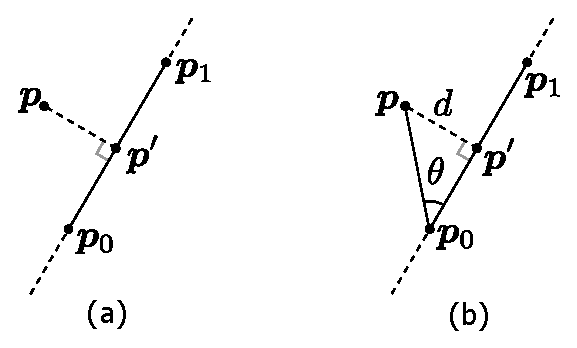
\includegraphics[width=0.4\linewidth]{chap03/Pointlinedistance.eps}
    \caption{(a)给定无限直线和点$\bm p$,则从该点到直线上
        最近点$\bm p'$的向量垂直于该直线。
        (b)因为该向量垂直,我们可以计算从直线上第一点到
        最近点$\bm p'$的距离为$d=\|\bm p-\bm p_0\|\cos\theta$。}
    \label{fig:3.23}
\end{figure}

\refeq{2.1}给出了两向量点积、它们的长度以及夹角余弦的关系。
特别地,它向我们展示了怎样计算从$\bm p_0$到$\bm p$的向量
与从$\bm p_0$到$\bm p_3$的向量之间夹角的余弦:
\begin{align*}
    \cos\theta=\frac{(\bm p-\bm p_0)\cdot(\bm p_3-\bm p_0)}{\|\bm p-\bm p_0\|\|\bm p_3-\bm p_0\|}\, .
\end{align*}

因为从$\bm p'$到$\bm p$的向量垂直于该直线(\reffig{3.23}(b)),
则我们可以计算沿直线从$\bm p_0$到$\bm p'$的距离为
\begin{align*}
    d=\|\bm p-\bm p_0\|\cos\theta=\frac{(\bm p-\bm p_0)\cdot(\bm p_3-\bm p_0)}{\|\bm p_3-\bm p_0\|}\, .
\end{align*}

最后,沿直线的参数偏移量$w$是$d$与直线长度的比值,
\begin{align*}
    w=\frac{d}{\|\bm p_3-\bm p_0\|}=\frac{(\bm p-\bm p_0)\cdot(\bm p_3-\bm p_0)}{\|\bm p_3-\bm p_0\|^2}\, .
\end{align*}

因为事实上相交坐标系中$\bm p=(0,0)$,所以$w$值的计算最后有所简化。
\begin{lstlisting}
`\initcode{Compute line w that gives minimum distance to sample point}{=}`
`\refvar{Vector2f}{}` segmentDirection = `\refvar{Point2f}{}`(cp[3]) - `\refvar{Point2f}{}`(cp[0]);
`\refvar{Float}{}` denom = segmentDirection.`\refvar{LengthSquared}{}`();
if (denom == 0)
    return false;
`\refvar{Float}{}` w = `\refvar{Dot}{}`(-`\refvar{Vector2f}{}`(cp[0]), segmentDirection) / denom;
\end{lstlisting}

贝塞尔曲线上到候选交点最近(假定)点的参数$u$坐标通过
沿该段$u$的范围线性插值算得。
给定该值,就能计算曲线在该点处的宽度。
\begin{lstlisting}
`\initcode{Compute u coordinate of curve intersection point and hitWidth}{=}`
`\refvar{Float}{}` u = `\refvar{Clamp}{}`(`\refvar{Lerp}{}`(w, u0, u1), u0, u1);
`\refvar{Float}{}` hitWidth = `\refvar{Lerp}{}`(u, `\refvar{common}{}`->`\refvar[CurveCommon::width]{width}{}`[0], `\refvar{common}{}`->`\refvar[CurveCommon::width]{width}{}`[1]);
`\refvar{Normal3f}{}` nHit;
if (`\refvar{common}{}`->`\refvar[CurveCommon::type]{type}{}` == `\refvar{CurveType}{}`::`\refvar{Ribbon}{}`) {
    `\refcode{Scale hitWidth based on ribbon orientation}{}`
}
\end{lstlisting}

对于\refvar{Ribbon}{}曲线,曲线并不总是朝向光线。
相反,它的朝向是在给定于每个端点处的曲面法线之间插值的。
这里,球面线性插值用于插值$u$处的法线(回想\refsub{四元数插值})。
再用规范化的射线方向与丝带朝向间的夹角余弦缩放曲线宽度,
这样它就反映了给定方向的曲线可见宽度。
\begin{lstlisting}
`\initcode{Scale hitWidth based on ribbon orientation}{=}`
`\refvar{Float}{}` sin0 = std::sin((1 - u) * `\refvar{common}{}`->`\refvar{normalAngle}{}`) *
    `\refvar{common}{}`->`\refvar{invSinNormalAngle}{}`;
`\refvar{Float}{}` sin1 = std::sin(u * `\refvar{common}{}`->`\refvar{normalAngle}{}`) *
    `\refvar{common}{}`->`\refvar{invSinNormalAngle}{}`;
nHit = sin0 * `\refvar{common}{}`->`\refvar[CurveCommon::n]{n}{}`[0] + sin1 * `\refvar{common}{}`->`\refvar[CurveCommon::n]{n}{}`[1];
hitWidth *= `\refvar{AbsDot}{}`(nHit, ray.`\refvar[Ray::d]{d}{}`) / rayLength;
\end{lstlisting}

为了最终将可能的相交处分类为命中或未命中,
必须用函数\refvar{EvalBezier}{()}
求贝塞尔曲线在$u$处的值
(因为控制点{\ttfamily cp}表示当前考虑的曲线段,
然而既然$w$在范围$[0,1]$内,在函数调用中使用$w$而不是$u$就很重要)。
曲线在该点的导数很快也会有用,所以现在记录下来。

我们想测试从$\bm p$到曲线上该点{\ttfamily pc}的
距离是否小于曲线宽度的一半。
因为$\bm p=(0,0)$,我们可以等价地测试从{\ttfamily pc}到原点
的距离是否小于宽度的一半,或者等价地,
平方距离是否小于宽度平方的四分之一。
如果该测试通过,最后一件事是检查交点是否在射线的参数$t$范围内。
\begin{lstlisting}
`\initcode{Test intersection point against curve width}{=}`
`\refvar{Vector3f}{}` dpcdw;
`\refvar{Point3f}{}` pc = `\refvar{EvalBezier}{}`(cp, `\refvar{Clamp}{}`(w, 0, 1), &dpcdw);
`\refvar{Float}{}` ptCurveDist2 = pc.x * pc.x + pc.y * pc.y;
if (ptCurveDist2 > hitWidth * hitWidth * .25)
    return false;
if (pc.z < 0 || pc.z > zMax)
    return false;
\end{lstlisting}

\refvar{EvalBezier}{()}计算簇$\bm p(u,u,u)$来求贝塞尔样条上的一点。
它也可选地返回曲线在该点处的导数\sidenote{译者注:读者可以动手验算一下。}。
\begin{lstlisting}
`\refcode{Curve Utility Functions}{+=}\lastcode{CurveUtilityFunctions}`
static `\refvar{Point3f}{}` `\initvar{EvalBezier}{}`(const `\refvar{Point3f}{}` cp[4], `\refvar{Float}{}` u,
        `\refvar{Vector3f}{}` *deriv = nullptr) {
    `\refvar{Point3f}{}` cp1[3] = { `\refvar{Lerp}{}`(u, cp[0], cp[1]), `\refvar{Lerp}{}`(u, cp[1], cp[2]),
                       `\refvar{Lerp}{}`(u, cp[2], cp[3]) };
    `\refvar{Point3f}{}` cp2[2] = { `\refvar{Lerp}{}`(u, cp1[0], cp1[1]), `\refvar{Lerp}{}`(u, cp1[1], cp1[2]) };
    if (deriv)
        *deriv = (`\refvar{Float}{}`)3 * (cp2[1] - cp2[0]);
    return `\refvar{Lerp}{}`(u, cp2[0], cp2[1]);
}
\end{lstlisting}

如果之前的测试都通过了,我们就找到了有效的相交,
现在可以计算交点的$v$坐标了。
曲线的$v$坐标在0到1内变化,曲线中心取值为0.5;
这里我们根据过曲线上的点{\ttfamily pc}和沿其导数的点的边函数
将交点$(0,0)$分类,决定交点在中心的哪边以及该怎样计算$v$。
\begin{lstlisting}
`\initcode{Compute v coordinate of curve intersection point}{=}`
`\refvar{Float}{}` ptCurveDist = std::sqrt(ptCurveDist2);
`\refvar{Float}{}` edgeFunc = dpcdw.x * -pc.y + pc.x * dpcdw.y;
`\refvar{Float}{}` v = (edgeFunc > 0) ? 0.5f + ptCurveDist / hitWidth :
                           0.5f - ptCurveDist / hitWidth;
\end{lstlisting}

最后,计算偏导数,相交处的\refvar{SurfaceInteraction}{}可以初始化了。
\begin{lstlisting}
`\initcode{Compute hit t and partial derivatives for curve intersection}{=}`
if (tHit != nullptr) {
    *tHit = pc.z / rayLength;
    `\refcode{Compute error bounds for curve intersection}{}`
    `\refcode{Compute $\partial$p/$\partial$u and $\partial$p/$\partial$v for curve intersection}{}`
    *isect = (*`\refvar{ObjectToWorld}{}`)(`\refvar{SurfaceInteraction}{}`(
        ray(pc.z), pError, `\refvar{Point2f}{}`(u, v), -ray.`\refvar[Ray::d]{d}{}`, dpdu, dpdv,
        `\refvar{Normal3f}{}`(0, 0, 0), `\refvar{Normal3f}{}`(0, 0, 0), ray.`\refvar[Ray::time]{time}{}`, this));
}
\end{lstlisting}

偏导数$\displaystyle\frac{\partial \bm p}{\partial u}$直接
来自于底层贝塞尔曲线的导数。
第二个偏导数$\displaystyle\frac{\partial \bm p}{\partial v}$则
基于曲线类型用不同方式计算。
对于丝带,我们有$\displaystyle\frac{\partial \bm p}{\partial u}$和
曲面法线,因此$\displaystyle\frac{\partial \bm p}{\partial v}$必须
是使得$\displaystyle\frac{\partial \bm p}{\partial u}\times\frac{\partial \bm p}{\partial v}=\bm n$的向量
且长度等于曲线宽度。
\begin{lstlisting}
`\initcode{Compute $\partial$p/$\partial$u and $\partial$p/$\partial$v for curve intersection}{=}`
`\refvar{Vector3f}{}` dpdu, dpdv;
`\refvar{EvalBezier}{}`(`\refvar{common}{}`->`\refvar{cpObj}{}`, u, &dpdu);
if (`\refvar{common}{}`->`\refvar[CurveCommon::type]{type}{}` == `\refvar{CurveType}{}`::`\refvar{Ribbon}{}`)
    dpdv = `\refvar{Normalize}{}`(`\refvar{Cross}{}`(nHit, dpdu)) * hitWidth;
else {
    `\refcode{Compute curve $\partial$p/$\partial$v for flat and cylinder curves}{}`
}
\end{lstlisting}

对于平坦和圆柱曲线,我们变换$\displaystyle\frac{\partial \bm p}{\partial u}$到相交坐标系。
对于平坦曲线,我们知道$\displaystyle\frac{\partial \bm p}{\partial v}$位于$xy$平面内、
垂直于$\displaystyle\frac{\partial \bm p}{\partial u}$且长度等于{\ttfamily hitWidth}。
我们可以用和之前求垂直于曲线段的边界边同样的方法求得2D垂直向量。
\begin{lstlisting}
`\initcode{Compute curve $\partial$p/$\partial$v for flat and cylinder curves}{=}`
`\refvar{Vector3f}{}` dpduPlane = (`\refvar[Transform::Inverse]{Inverse}{}`(rayToObject))(dpdu);
`\refvar{Vector3f}{}` dpdvPlane = `\refvar{Normalize}{}`(`\refvar{Vector3f}{}`(-dpduPlane.y, dpduPlane.x, 0)) *
                     hitWidth;
if (`\refvar{common}{}`->`\refvar[CurveCommon::type]{type}{}` == `\refvar{CurveType}{}`::`\refvar[CurveType::Cylinder]{Cylinder}{}`) {
    `\refcode{Rotate dpdvPlane to give cylindrical appearance}{}`
}
dpdv = rayToObject(dpdvPlane);
\end{lstlisting}

圆柱曲线的向量$\displaystyle\frac{\partial \bm p}{\partial v}$沿轴{\ttfamily dpduPlane}旋转
使其外观像圆柱体横截面。
\begin{lstlisting}
`\initcode{Rotate dpdvPlane to give cylindrical appearance}{=}`
`\refvar{Float}{}` theta = `\refvar{Lerp}{}`(v, -90., 90.);
`\refvar{Transform}{}` rot = `\refvar{Rotate}{}`(-theta, dpduPlane);
dpdvPlane = rot(dpdvPlane);
\end{lstlisting}

这里没有介绍的方法\refvar{Curve::Area}{()}首先
用其控制点连线长度近似曲线长度。
然后它再用该长度乘以其范围内宽度的均值以近似整个曲面面积。